\documentclass[a4paper,12pt]{report}
\usepackage[latin1]{inputenc}
\usepackage[catalan]{babel}
\language=1
\usepackage{amsmath}
\usepackage{amsfonts}
\usepackage{amssymb}
\usepackage[dvips]{graphicx}
%\usepackage{theorem}

\setlength{\parindent}{0pt}
\def\ll{\ifmmode{\mathchar"321C}\else%
l\discretionary{-}{l}{\kern-.12em\hbox{${\cdot}$}\kern-.13eml}\fi}
\def\LL{L\discretionary{-}{L}{\kern-.09em\hbox{${\cdot}$}\kern-.16emL}}
%%%%%%%%%%%%%%%%%%%%%%%%%%%%%%%%%%%
\newcommand{\Real}{\mathbb{R}}
\newcommand{\Ind}{\mathbf{1}}
\newcommand{\Alg}{{\cal A}}
\newcommand{\iid}{\stackrel{iid}{\sim }X}
\newcommand{\bX}{\mathbf{X}} %Una mostra, com un vector, en negreta. Majuscules
\newcommand{\bx}{\mathbf{x}}%Una mostra, com un vector, en negreta. Min�scules
\newcommand{\Sx}{\stackunder{\sim }{X}} %Una mostra, amb una tilde a sota. Majuscules
\newcommand{\sx}{\stackunder{\sim }{x}}%Una mostra, amb una tilde a sota. Min�scules

\newcommand{\Sample}{X_1,X_2,\dots,X_n}
\newcommand{\sample}{x_1,x_2,\dots,x_n}
\newcommand{\YSample}{Y_1,Y_2,\dots,Y_n}
\newcommand{\ysample}{y_1, y_2,\dots,y_n}
\newcommand{\Sumin}{{\sum_{i=1}^n}}
\newcommand{\Prodin}{{\prod_{i=1}^n}}
\newcommand{\Fnx}{F_n(x)}
\newcommand{\bias}{b_T(\theta)}
\newcommand{\te}{T}
\newcommand{\teX}{T(\bX)}
\newcommand{\tex}{t(\bx)}
%\newcommand{\T2}{\widehat{\theta}_2}
\newcommand{\modest}{\left\{ X\sim F_\theta:\theta\in\Theta\right\}}
\newcommand{\Mx}{\overline{x}}
\newcommand{\MX}{\overline{X}}
%\newcommand{\th}{\widehat{\theta}}
\newcommand{\beqa}{\begin{eqnarray*}}
\newcommand{\eeqa}{\end{eqnarray*}}
\newcommand{\bit}{\begin{itemize}}
\newcommand{\eit}{\end{itemize}}
\newcommand{\ben}{\begin{enumerate}}
\newcommand{\een}{\end{enumerate}}
%\renewcommand{\thesubsection}{\thesection-\Alph{subsection}}
\newcommand{\ze}{z_{2\alpha}}
%\newcommand{\zee}{z_{2\alpha}}
\newcommand{\zem}{z_{\alpha}}
%\newcommand{\te}{t_{\alpha}}
\newcommand{\tee}{t_{2\alpha}}
\newcommand{\tem}{t_{\alpha/2}}

\newcommand{\citalib}[6]{\bibitem{#1} #2\ (#3).\ {\em{ #4}}.\  #5. \ #6.}
%\citalib{Alcaide-92}     %paraula clau per a la cita
%{Alcaide, J.}            %autors
%{1996}                   %any
%{Metodolog!`a de la prog} %Titol
%{Mc Graw-Hill}           %Editorial
%{Madrid}                 %Lloc
\newcommand{\ds}{\displaystyle}
%\newcounter{thm}[section]
\newtheorem{theorem}{Teorema}[chapter]
\newtheorem{proof}{Demostraci\'{o}}
\newcounter{cor}[section]
\newtheorem{corollary}[cor]{Coro{\ll}ari}
%Inicialment ho feia aix\'{\i}
%\newcounter{examp}[subsection]
%\newtheorem{example}[examp]{Exemple}
%\newcounter{def}[section]
%\newtheorem{definition}[def]{Definici\'o}
%El Paco proposa canviar-ho a:
\newtheorem{teorema}{Teorema}[chapter]
%{\theorembodyfont{\rmfamily}%
\newtheorem{exercici}{Exercici [chapter]}
\newtheorem{example}{Exemple}[section]
\newtheorem{definition}{Definici\'o}[chapter]

\newcounter{prop}[chapter]
\newtheorem{proposition}[prop]{Proposici\'o}
\newcounter{lema}[chapter]
\newtheorem{lemma}[lema]{Lema}

\newcommand{\cinlaw}{\buildrel {\cal L} \over \longrightarrow }
\newcommand{\cinprob}{\buildrel {P} \over \longrightarrow }
\newcommand{\tendsto}{\stackunder{n\rightarrow \infty }{\longrightarrow}}

%%%Definit al Scientific Workplace
\def\stackunder#1#2{\mathrel{\mathop{#2}\limits_{#1}}}%
\def\dfrac#1#2{{\displaystyle {#1 \over #2}}}%
% Per generar documents pdf
%\pdfcompreslevel=9
%\pdfoutput=1
%
%Per incloure imatges
%
%\begin{figure}[hbtp]
%\vspace{-3cm} \special{center
%         ./IMATGES/CLINES.wmf,
%         \the\hsize 12cm}
%\vspace{12cm} \vspace{3cm} \caption{\sl } \label{Figura}
%\end{figure}
%\clearpage


\includeonly{tapa,EM2-Intro,EM2Cap1,EM2Cap2,EM2Cap3,EM2Cap4,EM2Cap5,EM2Cap6,EM2Cap7,EM2Cap8,EM2Bib}
%\includeonly{EM2Cap3}

\begin{document}
\thispagestyle{empty}
\vspace*{\stretch{1}}
\rule{\linewidth}{1mm}
\begin{center}
\textsf{\textbf{\Huge ESTAD�STICA MATEM�TICA II \\[5mm] APUNTS}}
\end{center}
\rule{\linewidth}{1mm}
\vspace*{\stretch{2}}
\begin{center}
\textsf{\textbf{\Large �lex S�nchez Pla \hspace{1.25cm} Francesc Carmona}}
\end{center}
\vspace*{2\baselineskip}
\begin{center}
\textsf{\textit{\Large
Departament d'Estad�stica}}
\end{center}
\vspace*{\stretch{2}}
\begin{center}
\includegraphics*{./imatges/logo_ub_nou.eps}
\end{center}
\vspace*{\stretch{2}}
\begin{center}
\textsf{\large Barcelona, 13 de febrer de 2002}
\end{center}

\thispagestyle{empty}
\null
\tableofcontents
\thispagestyle{empty}
\newpage
\section*{Presentaci�}

El material que es presenta a continuaci� s'ha originat en les
notes de classe de l'assignatura \emph{Estad�stica Matem�tica} que
hem impartit a la Diplomatura d'Estad�stica des del seu inici a la
Universitat de Barcelona.

L'objectiu d'aquests apunts no �s substituir els llibres citats a
la bibliografia sin�, m�s aviat, servir com a guia d'estudi per
tal que els estudiants puguin repassar els raonaments i els
c�lculs fets a classe i assegurar-se de que ho entenen tot
correctament.

Aquest document �s una versi� preliminar i, com a tal, pot
contenir algunes errates. Si ens hem animat a publicar-ho de forma
electr�nica, ha estat amb la idea que pugui resultar d'utilitat a
aquells a qui va destinat, no en un futur incert sin� des d'ara
mateix. Ens agradaria que ens f�ssiu arribar qualsevol errada,
errata o comentari.

\bigskip
Barcelona, 13 de febrer de 2002

\bigskip
�lex S�nchez Pla (alex@bio.ub.es) \\
Francesc Carmona (carmona@bio.ub.es)\\
Departament d'Estad�stica\\
Universitat de Barcelona

\thispagestyle{empty}
\newpage

%\chapter{INFER�NCIA ESTAD�STICA. INTRODUCCI�}
\setcounter{page}{1}
\chapter{INFER�NCIA, MOSTRATGE I DISTRIBUCIONS MOSTRALS}

\section{Infer�ncia estad�stica}

Per comen�ar anem a definir quin �s l'�mbit d'estudi de la
infer�ncia estad�stica des de la seva relaci� amb el c�lcul de
probabilitats. El c�lcul de probabilitats proporciona una teoria
matem�tica que permet analitzar (o modelitzar) les propietats dels
fen�mens on interv� l'atzar.

El c�lcul de probabilitats utilitza com a model b�sic per a
qualsevol situaci� aleat�ria el concepte d'espai de probabilitats
$(\Omega ,\Alg,P)$ i una variable aleat�ria $X:\Omega \rightarrow
\Real$ definida sobre ell.

El coneixement de la distribuci� de la variable aleat�ria
permet:
\begin{enumerate}
\item  \textbf{An�lisis deductiva de situacions.}
\textit{Per exemple: si assumim que el pes dels nadons es
distribueix segons una distribuci� $N(\mu =\textrm{\emph{ 3
kg}},\sigma =\textrm{\emph{0.25 kg}})$ ens pot interessar calcular
la probabilitat que un nad� pesi entre $2.9$ i $\,3.1$ \emph{kg},
o trobar uns valors centrats en la mitjana entre els quals esperem
que es trobin el 10\% (25\%, 50\%, 95\%,$\dots$) dels nadons.}

\item  \textbf{Modelitzaci� de situacions aleat�ries.}
\textit{Per exemple: si assumim que el temps, en anys, fins que
s'espatlla una component d'un ordinador es distribueix segons una
distribuci� exponencial $T\sim \xi (\lambda=0.3 )$ ens pot
interessar calcular la probabilitat que una component donada duri
m�s de $4$ anys.}
\end{enumerate}

En els casos anteriors ens trobem en una situaci� molt usual, on
ja disposem d'un model sobre el qual efectuem els c�lculs, per�
del qual desconeixem la proced�ncia. Sembla raonable, i de fet �s
precisament aix�, que si volem adaptar un model a una situaci�
haguem de basar-nos �nicament en les observacions del fenomen.

Si volem saber c�m es distribueixen els pesos dels nadons
n'agafarem uns quants, els pesarem i despr�s mirarem la
distribuci� d'aquests. Pot ser que no calgui pesar tots els nadons
(de fet no �s possible!), per� tampoc �s possible deduir la llei
per consideracions purament te�riques.

Ara, enlloc de partir d'un espai de probabilitats partirem d'unes
observacions $\left( x_1,...,x_n\right)$ i l'objectiu que
perseguirem ser� obtenir informaci� sobre la distribuci� de
probabilitats d'un fenomen a partir d'una observaci� no exhaustiva
d'aquest.

\section{Problemes d'infer�ncia estad�stica}

Hem presentat com a objectiu de la infer�ncia estad�stica
induir propietats del model probabil�stic que representa la
poblaci� a partir d'un conjunt d'observacions.

Segons el tipus de conclusi� que vulguem extreure
diferenciarem diferents tipus de problemes:

\begin{enumerate}
\item  Si volem utilitzar la informaci� proporcionada per la mostra per
obtenir una pron�stic num�ric �nic (�s a dir una �nica aproximaci�
num�rica) d'una o m�s caracter�stiques de la poblaci� tenim un
problema d'\emph{estima\-ci� puntual}.

\item  Si volem obtenir informaci� sobre un rang de valors dins del qual
puguem afirmar, amb un cert grau de confian�a, que podem atrapar
un par�metre desconegut de la distribuci� parlem d'\emph{estimaci�
per interval}.

\item  Si el que volem fer �s decidir si podem acceptar o hem de
rebutjar una afirmaci� sobre la distribuci� de
probabilitat del fenomen estudiat parlem de \emph{contrast
d'hip�tesis}. Aquest contrast pot ser:

\begin{itemize}
\item  Param�tric: si l'afirmaci� (la hip�tesi)\ es refereix als
par�metres de la distribuci�.

\item  No param�tric: si l'afirmaci� �s sobre la forma de la
distribuci�.
\end{itemize}
\end{enumerate}

\section{Distribuci� de la poblaci�}

Tot problema d'infer�ncia est� motivat per un cert grau de
desconeixement de la llei de probabilitats que regeix un
determinat fenomen aleatori.

El cas m�s senzill amb el que ens trobem �s quan ens interessa una
certa variable $X$ amb una funci� de distribuci� $F$ desconeguda
en major o menor grau.

La distribuci� que te�ricament segueix la variable d'inter�s $X$
en la poblaci� rep el nom de \emph{distribuci� te�rica} o
\emph{distribuci� de la poblaci�}. La distribuci� de la poblaci�
�s important ja que sovint es fa servir per determinar la
distribuci� d'alguna caracter�stica dels individus d'una poblaci�.

En els models de la infer�ncia estad�stica indiquem el relatiu
grau de desconeixement sobre la distribuci� $F$ en funci� de la
seva pertinen�a a una fam�lia $\mathcal{F}$ de distribucions. Per
aix�, enlloc d'explicar que $X\sim F=F_0$ indicarem que $X\sim F
\in \mathcal{F}$, on $\mathcal{F}$ pot ser un conjunt m�s o menys
extens de distribucions de probabilitat com totes les
\emph{distribucions normals} o les \emph{distribucions
sim�triques} o les \emph{distribucions discretes sobre
$\mathbb{N}$}.

Moltes vegades la distribuci� poblacional $F$ est� completament
especificada excepte pel valor d'algun par�metre o par�metres. En
aquest cas podem concretar m�s la forma de la fam�lia de
distribucions:
\[
X\sim F\in \mathcal{F}=\left\{ F_{\theta} :\theta \in \Theta
\subset \Real^k\right\}
\]
on $\Theta$ �s l'espai dels $k$ par�metres.

La fam�lia de possibles distribucions de probabilitat per a $X$
s'anomena, gen�ricament, \emph{model estad�stic} i s'indica com: $\modest$.

Veiem alguns exemples.

\begin{example}
Suposem que $X$ representa la durada d'un component elec\-tr�\-nic
que no envelleix, nom�s s'espatlla. �s a dir, si en un instant $t$
est� funcionant el seu estat �s el mateix que en qualsevol moment
del passat i la distribuci� del temps fins que s'espatlli �s la
mateixa que al principi. Aquesta propietat s'anomena manca de
mem�ria.

Un model raonable per aquesta situaci� el d�na la distribuci� de
Weibull que, en aquest cas, podem definir a trav�s de la seg�ent
funci� de densitat:
\[
f_{\theta}(x) =\left\{
\begin{array}{ll}
\alpha\beta x^{\beta-1} e^{-\alpha x^\beta} & \textrm{si $x\ge 0$}\\
0 & \textrm{si $x<0$}
\end{array}\right.
\]
La fam�lia de distribucions associada �s $$\mathcal{F}=\left\{
F_\theta : \theta=(\alpha,\beta) \in (0,\infty )\times (0,\infty
)\right\}$$
\end{example}

\begin{example}
Suposem que volem determinar la massa d'un cert tipus de
part�cules elementals a partir de les observacions en una cambra
de bombolles. En cada observaci� obtenim una dada de la massa de
la part�cula $x_i$ i associada amb ella un cert error de mesura
$\varepsilon$. Si la massa comuna de cadascuna d'elles �s $\mu$
llavors podem escriure:
\[
x_i=\mu +\varepsilon _i \qquad i=1,...,n
\]
on la distribuci� $\varepsilon _i\sim F$ �s desconeguda.
El nostre objectiu �s obtenir informaci� sobre $F$.

Si admetem que $P(\varepsilon_i<0)=P(\varepsilon_i>0)$, segons
el grau d'exig�ncia que volem tenir, podem suposar:
\begin{itemize}
\item  Amb un enfocament d'\emph{infer�ncia param�trica}:
\[
X\sim F\in\mathcal{F}=\{ N(0,\sigma) :\sigma\in\Real^{+}\}
\]
\item  Amb un enfocament d'\emph{infer�ncia no param�trica}:
\[
X\sim F \in\mathcal{F}=\{\text{\emph{Distribucions sim�triques}} \}
\]
\end{itemize}
\end{example}

\section{Mostra aleat�ria simple}

\subsection{Definici�}
Per estudiar un problema d'infer�ncia estad�stica analitzem una
mostra de mida $n$. Es tracta d'escollir $n$ individus o elements
de la poblaci� $\Omega$
\[
\omega_1,\omega_2,\dots,\omega_n
\]
que siguin representatius. El valor de $n$ i la forma d'elecci�
dels individus de la mostra �s una materia d'Estad�stica anomenada
\emph{Mostratge estad�stic}. Per ara i per simplificar, nom�s cal
dir que l'elecci� es fa de forma que tots els individus tenen la
mateixa probabilitat de ser presents a la mostra, si cal amb
reempla�ament, i que el valor de $n$ est� donat.

En realitat, el que ens interessa veritablement, no s�n els
individus de la mostra sin� les mesures d'una caracter�stica $X$
sobre ells. �s a dir, els valors d'una variable aleat�ria $X$
sobre aquests individus
\[
X(\omega_1)=x_1,X(\omega_2)=x_2,\dots,X(\omega_n)=x_n
\]
Tamb� podem pensar que els valors mostrals $x_1,x_2,\dots,x_n$ s�n
generats directament des de la variable aleat�ria. En tot cas, els
valors mostrals no s�n �nics i podem generar v�ries mostres
\[
\begin{array}{ccccc}
x_1^1 & x_2^1 & x_3^1 & \dots & x_n^1 \\
x_1^2 & x_2^2 & x_3^2 & \dots & x_n^2 \\
\vdots & \vdots & \vdots & & \vdots \\
x_1^s & x_2^s & x_3^s & \dots & x_n^s
\end{array}
\]
Si tots els valors s�n independents, de la mateixa forma que
$x_1,x_2,x_3,\dots,x_n$ �s una mostra generada per $X$, podem
considerar tots els $x_1^i\quad i=1,...,s$ provinents d'una
variable aleat�ria $X_1$ amb la mateixa distribuci� que $X$
$X_1\stackrel{d}{=}X$ i que genera els primers valors, els
$x_i^2$ provinents d'una variable aleat�ria $X_2\stackrel{d}{=}X$
que genera els segons i aix� successivament.

Tot aix� ens porta a definir el concepte de mostra
aleat�ria d'una forma molt convenient per treballar amb ella:
\begin{definition}
Una mostra aleat�ria simple de mida $n$ d'una variable
alea\-t�\-ria $X$ amb distribuci� $F$ �s una co{\ll}ecci� de $n$
variables aleat�ries independents $X_1,X_2,\dots,X_n$ amb la
mateixa distribuci� $F$ que $X$. Aix� se sol indicar com:
\[
\bX =\Sample \stackrel{i.i.d.}{\sim}X
\]
\end{definition}

\begin{definition}
El conjunt $(x_1,x_2,\dots,x_n)\in\Real^n$ d'observacions
concretes de $\Sample$ s'anomena \emph{realitzaci�} de la mostra.
\end{definition}

\subsection{Distribuci� de la mostra}

Una mostra aleat�ria simple, com a vector aleatori $n$-dimensional
que �s, t� una distribuci� conjunta o \emph{distribuci� de la
mostra} que dep�n de $F$, per� que �bviament �s diferent, ja que
en particular $X$ i $\bX$ tenen dimensions diferents. Ara b�,
gr�cies a la independ�ncia de les variables $\Sample$, la funci�
de distribuci� conjunta de $\bX$, que podria ser molt complicada,
pren una forma molt senzilla. En resum:
\begin{definition}
S'anomena distribuci� de la mostra d'una variable aleat�ria $X\sim
F$ a la distribuci� del vector aleatori $n$-dimensional
$(\Sample)$
\[
G(x_1,x_2,...,x_n)=F(x_1) F(x_2)\cdots F(x_n)
\]
\end{definition}

En els casos particulars en que $X$ sigui discreta o absolutament
cont�nua la distribuci� conjunta de la mostra sol expressar-se mitjan�ant la funci� de massa de probabilitat o la funci�
de densitat:
\begin{itemize}
\item  Per a variables discretes:
\begin{eqnarray*}
p_G(\sample)&=& P(X_1=x_1,X_2=x_2,\dots,X_n=x_n)\\
&=&  \prod_{i=1}^n P\left( X=x_i\right)=\prod_{i=1}^n p_F\left(
x_i\right),
\end{eqnarray*}
\item Per a variables absolutament cont�nues:
$$g(x_1,x_2,\dots,x_n)=\prod_{i=1}^n f(x_i)$$
\end{itemize}

\begin{example}
Una moneda t� una probabilitat $\theta$ de sortir cara.
Volem estudiar la variable aleat�ria:
\[
X=\left\{
\begin{array}{cc}
1 & \textrm{si surt cara} \\
0 & \textrm{si surt creu}
\end{array}
\right.
\]
amb densitat $P\{ X=1\} =\theta$, $P\{ X=0\} =1-\theta$. �s a dir
\[
X\sim F_\theta \in
\mathcal{F}=\left\{ F_\theta=B(1,\theta) : \theta\in(0,1)\right\}
\]
Suposem que fem tres llan�aments. Les possibles mostres s�n:
\[
\begin{array}{cccc}
  X_1 & X_2 & X_3 & \mbox{Probabilitat} \\
  \hline
  1 & 1 & 1 &  \theta ^3\\
  1 & 0 & 0 & \theta \left( 1-\theta \right) ^2 \\
  0 & 1 & 0 & \theta \left( 1-\theta \right) ^2\\
  0 & 0 & 1 & \theta \left( 1-\theta \right) ^2 \\
  1 & 0 & 1 & \theta ^2\left( 1-\theta \right) \\
  1 & 1 & 0 & \theta ^2\left( 1-\theta \right)\\
  0 & 1 & 1 & \theta ^2\left( 1-\theta \right) \\
  0 & 0 & 0 & \left( 1-\theta \right) ^3
\end{array}
\]

El mostratge ha especificat la distribuci� conjunta de la mostra a
trav�s de la distribuci� desconeguda $F_\theta$. Si escrivim la
funci� de probabilitats de la variable aleat�ria com $f_\theta(x)
=\theta^x(1-\theta)^{1-x}$, llavors la funci� de probabilitats de
la mostra la podem expressar com:
\[
g_\theta(x_1,x_2,x_3)=\theta^{x_1+x_2+x_3}(1-\theta)^{3-(x_1+x_2+x_3)}
\]
\end{example}

\section{Estad�stics}

\subsection{Definici�}

Per aconseguir l'objectiu de realitzar infer�ncies sobre la
poblaci� a partir de la mostra ens solem basar en la realitzaci�
de c�lculs sobre la mostra per mirar d'obtenir la informaci� que
desitgem. En aquest proc�s apareixen els conceptes d'estad�stic i
el cas particular, que m�s ens interessa a nosaltres, d'estimador.
Un estad�stic �s una funci� de la mostra que no dep�n del valor
del par�metre.

\begin{definition}
Donada una mostra aleat�ria simple $\Sample$ i una funci�
mesurable $T:\Real^n\longrightarrow \Real^k$, llavors $T(\Sample)$
�s un vector aleatori (variable aleat�ria quan $k=1$). Si $T$ no
dep�n de $\theta$ (on $\theta$ �s un par�metre a especificar en
$F_\theta$), llavors $T$ rep el nom d'estad�stic.
\end{definition}

Nom�s pel seu nom, sembla evident que un estimador d'un par�metre
$\theta$ ser� alguna funci� de la mostra que serveixi per
aproximar, en algun sentit, el valor desconegut de $\theta$. Si
afegim la condici� raonable que un estimador no pugui prendre
valors que no pot prendre el par�metre podem donar la seg�ent
definici�.
\begin{definition}
Un estimador d'un par�metre $\theta$ �s un estad�stic $T$ el
recorregut del qual �s l'espai dels par�metres, �s a dir:
\[
\begin{array}{rcccl}
T: & \Real^n & \longrightarrow & \Real^k & \\
& (\sample) & \longrightarrow & (t_1,\dots,t_k) &\in\Theta\subset
\Real^k
\end{array}
\]
\end{definition}

\subsection{Distribuci� en el mostratge d'un estad�stic}

Donat un estad�stic $T(\Sample)$ ens interessa con�ixer la seva
distribuci� de probabilitat, ja que per fer infer�ncia ens caldr�
fer c�lculs del tipus
$$P\left[T(\Sample)>t_0\right]$$
La distribuci� de probabilitat de l'estad�stic s'anomena
distribuci� mostral o distribuci� en el mostratge de l'estad�stic.
Trobar-la �s un problema que pot ser des de bastant senzill fins a
extremadament complicat. Algunes de les t�cniques utilitzades per
mirar de resoldre'l s�n les seg�ents:
\begin{itemize}
\item  �s de la t�cnica de canvi de variable.
\item  �s de la funci� generatriu de moments.
\item  Aplicaci� del Teorema Central del L�mit.
\end{itemize}

\begin{example}
Sigui $X\sim F_\theta$ una variable aleat�ria absolutament
cont�nua amb densitat
\[
f_\theta(x)=e^{-(x-\theta)}e^{-e^{-(x-\theta)}}\quad \theta\in\Real
\]
i considerem l'estad�stic
\[
T(\Sample)=\Sumin e^{-X_i}
\]
Si apliquem el
teorema de canvi de variable unidimensional, s'obt� f�cilment que
la variable aleat�ria $Y=e^{-X}$ segueix una distribuci� exponencial de
par�metre $e^{-\theta}$, d'on la suma seguir� una distribuci�
gamma $T\sim \Gamma(e^{-\theta},n)$.
\end{example}

\begin{example}
Suposem que $X$ representa el nombre d'avaries en una m�\-qui\-na al
cap d'un mes. Aquest valor varia mes a mes. Sigui $\bar{X}$ la
mitjana d'avaries en $n$ mesos. Si $X$ segueix una
distribuci� de Poisson $P(\lambda)$, quina �s la distribuci� de $\bar{X}$?

Com que la suma de Poisson i.i.d. �s $\sum_{i=1}^n X_i\sim
P(n\lambda)$
\[
P\left[\bar{X}=r\right] =P\left[ \sum_{i=1}^n
X_i=nr\right] =\frac{e^{-n\lambda }\left( n\lambda \right)
^{nr}}{\left( nr\right) !} \]
\end{example}

Com passa en aquest exemple, un dels estad�stics pel qual sovint
desitgem calcular la distribuci� en el mostratge �s la mitjana
aritm�tica. Una manera �til de fer-ho �s amb la funci� generatriu
de moments i l'aplicaci� del seg�ent lema.
\begin{lemma}
Si $X$ �s una v.a. amb $M_X(t)$ com funci� generatriu de
moments, llavors la f.g.m. de $\bar{X}_n=\frac
1n \Sumin X_i$ �s
\[
M_{\bar{X}_n}(t)=\left[M_X(t/n)\right]^n
\]
\end{lemma}

\emph{Demostraci�:}

La demostraci� �s immediata a partir de la definici� o
per les propietats de la funci� generatriu de moments.

Si apliquem directament la definici� de la f.g.m tenim:
\[
\begin{split}
E(e^{t\bar{X}_n}) &= E(e^{t\frac 1n\Sumin X_i})
= E\left (\Prodin e^{\frac tnX_i}\right)
=\Prodin E\left(e^{\frac tnX_i}\right)\\
&=\Prodin M_{X_i}(t/n)=\left[ M_X(t/n)\right]^n
\end{split}
\]

Si fem servir les propietats de la f.g.m. tenim:
\begin{enumerate}
\item  Donat que $M_{aX}(t)=M_X(at)$ i si $a=\frac 1n$, llavors
$M_{\bar{X}}(t)=M_{\sum_{i=1}^n X_i}(t/n)$.
\item  $M_{\sum_{i=1}^n X_i}(t/n)\stackrel{\mbox{ind}}{=}%
\Prodin M_{X_i}(t/n)\stackrel{\mbox{id}}{=}\left[ M_X(t/n)\right]^n$.
\end{enumerate}

\begin{example}
Per a una variable aleat�ria $X\sim N(\mu,\sigma)$ i per tant
$M_X(t)=\exp \left(t\mu +\frac{t^2\sigma^2}2\right)$, aleshores
\[
\begin{split}
M_{\bar{X}_n}(t)&=\left[\exp\left(\frac{t\mu}{n}+\frac{t^2\sigma^2}{n^2 2}\right) \right]^n\\
&=\exp\left[ n\left(\frac{t\mu}n
+\frac{t^2\sigma^2}{n^2 2}\right)\right] \\
&=\exp\left[t\mu+\frac 12 t^2\left(\frac{\sigma}{\sqrt{n}}\right)^2\right]
\end{split}
\]
que �s la funci� generatriu de moments d'una
variable $N(\mu,\sigma/\sqrt{n})$.
\end{example}

\section{La distribuci� emp�rica}

\subsection{Definici�}

En l'apartat anterior hem vist que a partir d'una mostra
$X_1,X_2,\dots,X_n$ t� inter�s considerar la distribuci� mostral
com la distribuci� conjunta del vector aleatori
$(X_1,X_2,\dots,X_n)$, sense que intervingui una realitzaci�
concreta de la mostra $x_1,x_2,\dots,x_n$. Un enfocament diferent
consisteix en associar una distribuci� particular directament a
les observacions $x_1,x_2,\dots,x_n$ amb la pretensi� que, en tant
que la mostra ``representa'' la v.a.$\ X$, aquesta distribuci�
associada a la mostra $F_n(x)$ emuli la distribuci� de la
poblaci�. Aquesta distribuci� s'anomena distribuci� emp�rica o
distribuci� mostral i es defineix aix�:
\[
F_n(x)=\frac{k(x)}{n}
\]
on $k(x)$ �s el nombre de dades mostrals menors o iguals que $x$.
A la pr�ctica es construeix per ordenaci� de la mostra \[
x_1,x_2,\dots,x_n
\longrightarrow x_{(1)}\le x_{(2)}\le \dots\le x_{(n)}
\]
i amb la seg�ent definici�:
\[
F_n(x) =\left\{
\begin{array}{ll}
0 & \mbox{si $x<x_{(1)}$} \\
\frac kn & \mbox{si $x_{(k)}\le x < x_{(k+1)}$} \\
1 & \mbox{si $x_{(n)}\le x$}
\end{array}
\right.
\]

\begin{example}
Extra\"{i}em una mostra i obtenim:

\begin{center}
\begin{tabular}{|c|c|c|c|c|c|c|}\hline
$x_1$ & $x_2$ & $x_3$ & $x_4$ & $x_5$ & $x_6$ & $x_7$ \\
$5.1$ & $3.4$ & $1.2$ & $17.6$ & $2.1$ & $16.4$ & $4.3$ \\ \hline
\end{tabular}
\end{center}

Un cop ordenada ens queda:
\begin{center}
\begin{tabular}{|c|c|c|c|c|c|c|}\hline
$x_{(1)}$ & $x_{(2)}$ & $x_{(3)}$ & $x_{(4)}$ & $x_{(5)}$ & $x_{(6)}$ &
$x_{(7)}$ \\
$x_3$ & $x_5$ & $x_2$ & $x_7$ & $x_1$ & $x_6$ & $x_4$ \\
$1.2$ & $2.1$ & $3.4$ & $4.3$ & $5.1$ & $16.4$ & $17.6$ \\ \hline
\end{tabular}
\end{center}
i si fem la representaci� gr�fica:
\begin{figure}[h]
\begin{center}
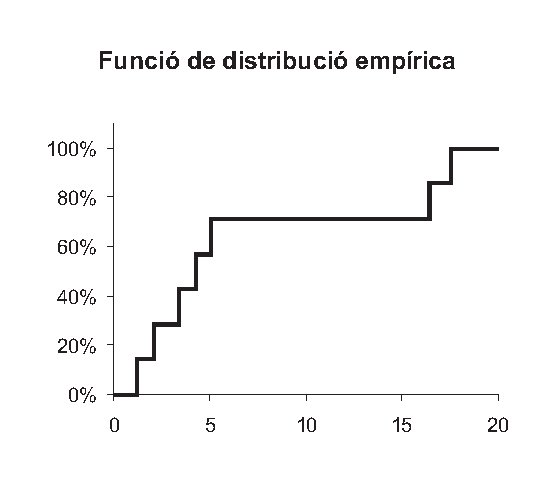
\includegraphics{./imatges/FdDEmp.eps}
\end{center}
\caption{Funci� de distribuci� emp�rica amb les dades de l'exemple}
\end{figure}
\end{example}

La distribuci� emp�rica reflecteix exclusivament els valors
observats a la mostra i per tant no es relaciona directament
ni amb la
distribuci� conjunta de la mostra $G(\sample)$ ni amb
la distribuci� de la poblaci� $F$. Malgrat aix�,
com �s raonable esperar, $F_n(x)$ proporciona una imatge
aproximada de la distribuci� de la poblaci� d'on s'ha
extret la mostra.

\subsection{Relaci� entre la distribuci� emp�rica i la poblacional}

L'estudi de la relaci� entre $F_n(x)$ i $F(x)$ es pot fer des de
diversos punts de vista. Podem considerar $F_n(x)$ com un
estad�stic o com una distribuci�.

Si considerem que $F_n(x)$ representa la freq��ncia relativa en la
mostra de l'esdeveniment $[X\le x]$ que t� probabilitat $F(x)$,
llavors �s un estad�stic. Aleshores, t� sentit que considerem la
seva distribuci� en el mostratge, $P[F_n(x)\leq z]$ i que estudiem
els moments d'aquesta distribuci�. En aquest cas tamb� t� sentit
aplicar les lleis dels grans nombres i determinar sota quines
condicions es verifica que $F_n(x) \longrightarrow F(x)$ en
probabilitat o quasi-segurament.

Si considerem que $F_n(x)$ representa directament una distribuci�
de probabilitat, definida sobre el conjunt $\{(\sample)\}$ t�
sentit que estudiem els seus moments, �s a dir, els de la variable
que la t� per distribuci�. Si la tractem com una distribuci� de
probabilitat tamb� t� sentit estudiar la seva converg�ncia en
distribuci�.

\subsubsection{L'estad�stic $F_n(x)$}

Per operar m�s f�cilment amb ella, podem escriure $\Fnx$
com:
$$
\Fnx=\frac 1n \Sumin \mathbf{1}_{[X_i\leq x]}(x)=\frac 1n \Sumin
W_i(x)
$$
i per simplificar la notaci� posarem $W_i$ enlloc de $W_i(x)$.

En l'exemple anterior, si $x=10$ tenim $W_1=W_2=W_3=W_5=W_7=1$,
$W_4=W_6=0$ i per tant $F_n(10)=5/7$.

Tal com hem definit $W_i$, aquest val $1$ si $X_i\leq x$ i 0 si
$X_i>x$, �s a dir
$$
W_i=\left\{
\begin{array}{ll}
1 & \mbox{amb $P[W_i=1] =P[X_i\leq x]=F(x)$} \\
0 & \mbox{amb $P[W_i=0] =1-P[X_i\leq x]=1-F(x)$}
\end{array}
\right.
$$
de forma que resulta clar que
$$
W_i\sim B(1,F(x)) \quad\mbox{de manera que}\quad
\Sumin W_i\sim B(n,F(x))
$$
i la variable $\frac 1n \Sumin W_i$ pren els valors
$0,\frac 1n,\frac 2n,\dots,\frac{n-1}n,1$ amb probabilitats definides per la distribuci� binomial $B(n,F(x))$.

De la representaci� anterior �s immediat que si posem $Y\sim
B(n,p)$ on $p=F(x)$, tenim:
\[
\begin{split}
E(\Fnx) &= E\left (\frac Yn\right)=\frac 1n
E(Y)=\frac 1n np=p=F(x) \\
\textrm{var}(\Fnx) &= \textrm{var}\left(\frac Yn\right)= \frac
1{n^2}\textrm{var}(Y)=\frac{npq}{n^2}=\frac{pq}n
=\frac{\Fnx\cdot(1-\Fnx)}{n^2}
\end{split}
\]

La v.a.$\ \Fnx$ �s un estad�stic que pren valors sobre el mateix
conjunt que $F(x)$ i, per tant, �s un estimador en el sentit
definit m�s amunt. �s d'esperar que $\Fnx$ s'apropi a $F(x)$ en
algun sentit. Per aplicaci� de les lleis dels grans nombres, i un
cop vista la representaci� de $F_n(x)$ com un promig de variables
i.i.d.$\ B(1,p)$, �s immediat que $F_n(x) \longrightarrow F(x)$ en
probabilitat i quasi-segurament.

El resultat anterior es refor�a si estudiem l'aproximaci� de
$F_n(x)$ a $F(x)$ a trav�s de l'estad�stic de Kolmogorov
\[
D_n=\sup_x |F_n(x)- F(x)|
\]
Es demostra\footnote{Veieu: \emph{Estad�stica}. Fortiana, J. i
Nualart, D. Publicacions U.B.} (Teorema de Glivenko-Cantelli) que
$F_n(x)$ convergeix a $F(x)$ quasi segurament i uniformement en
$x$, �s a dir
\[
P\left[ \lim D_n=0\right] =1
\]
Pel que fa a la
converg�ncia en distribuci� de $F_n(x)$ podem enunciar la seg�ent propietat.

\begin{proposition}
Sigui $\sample$ una realitzaci� d'una mostra aleat�ria simple de
la distribuci� $F$ i sigui $F_n(x)$ la seva funci� de distribuci�
emp�rica. L'estad�stic $F_n(x)$ t� una distribuci� de probabilitat
asimpt�ticament normal
$$
F_n(x)\sim AN\left(F(x),\sqrt{\frac{F(x)\cdot(1-F(x))}{n}}\right)
$$
\end{proposition}
La demostraci� �s immediata si considerem la representaci� de
$\Fnx$ com suma de variables aleat�ries i.i.d. i apliquem el
Teorema Central del L�mit.

\subsubsection{La distribuci� de probabilitat $\Fnx$}
Si considerem $\Fnx$ com una distribuci� de probabilitat, t�
sentit estudiar els moments de la variable que t� a $\Fnx$ per
funci� de distribuci�, aix� com la seva converg�ncia en
distribuci�. Com a conseq��ncia d'alguns dels resultats anteriors,
$\Fnx$ convergeix en distribuci� cap a la distribuci� poblacional.
Es pot justificar simplement tenint en compte que la converg�ncia
en probabilitat implica la converg�ncia en distribuci�.

Pel que fa als moments de la distribuci� emp�rica la seg�ent
secci� estudia els moments mostrals que s�n, de fet, els moments
d'una variable aleat�ria que tingui a $\Fnx$ com funci� de
distribuci�.

\section{Els moments mostrals}

\subsection{Definici�}

Sigui $F_n$ la v.a. que t� $F_n(x)$ per distribuci�. La funci� de
densitat de probabilitat de $F_n$ �s una densitat discreta que
assigna probabilitats $1/n$ a cadascuna de les observacions
mostrals $\sample$. Aix� doncs, t� sentit que calculem els seus
moments que es coneixen com a \emph{moments mostrals} $a_k$ i
tamb� els seus \emph{moments mostrals centrats respecte la
mitjana} $b_k$.
\[
\begin{split}
a_k&= E(F_n^k)=\sum_{i=1}^n x_i^k\cdot P(F_n=x_i) =
\sum_{i=1}^n x_i^k\cdot \frac 1n=\frac 1n\sum_{i=1}^n
x_i^k\\
b_k&=\frac 1n\sum_{i=1}^n (x_i-\bar{x})^k
\end{split}
\]
Observem que dues mesures conegudes
de l'estad�stica descriptiva adquireixen un significat
diferent:
\begin{itemize}
\item  Mitjana mostral = Mitjana de la distribuci� mostral
$$a_1=\frac 1n\sum_{i=1}^n x_i$$
\item  Vari�ncia mostral = Vari�ncia de la
distribuci� mostral
$$b_2=\frac 1n\sum_{i=1}^n (x_i-\bar{x})^2$$
\end{itemize}

\subsection{Distribuci� en el mostratge dels moments mostrals}

Donada una m.a.s.$\ X_1,X_2,\dots,X_n$, els moments mostrals s�n
estad�stics i, com a tals, tenen la seva distribuci� en el
mostratge. Per exemple, $a_k = \frac 1n \Sumin X_i^k$.

La distribuci� en cada cas pot ser complexa i dependre de la
distribuci� poblacional subjacent.

El que s� �s possible calcular s�n els moments dels moments
mostrals o, m�s ben dit, els moments de les distribucions en el
mostratge dels moments mostrals.

\begin{enumerate}
\item  Si considerem $a_k=\frac 1n\sum_{i=1}^n X_i^k$ i escrivim
$\alpha_k=E(X^k)$ com el moment poblacional d'ordre $k$, tenim:
\[
\begin{split}
E(a_k)&= E\left( \frac 1n \Sumin X_i^k\right) =\frac
1n\cdot n\cdot\alpha_k=\alpha_k \\
\mathrm{var}(a_k) &=\mathrm{var}\left(\frac 1n \Sumin
X_i^k\right)= \frac 1{n^2}\sum_{i=1}^n \mathrm{var}\left(
X_i^k\right) =\frac 1n \mathrm{var}(X^k) \\
&=\frac 1n\left[ E(X^{2k}) -(E(X^k))^2\right] =
\frac{\alpha_{2k}-\alpha _k^2}n
\end{split}
\]
\item  Si considerem $s^2=b_2=\frac 1n\sum_{i=1}^n (X_i-\bar{X})^2=
\frac 1n\sum_{i=1}^n X_i^2-\bar{X}^2$, podem calcular:
\[
\begin{split}
E(s^2) &= \frac 1n\sum_{i=1}^n
E(X_i^2) - E(\bar{X})^2
=\alpha_2- \left(\frac{\sigma ^2}n+\mu ^2\right) \\
&=(\sigma^2+\mu^2) -\left(\frac{\sigma^2}n+\mu^2\right)
=\frac{n-1}n\sigma^2
\end{split}
\]
El c�lcul de la vari�ncia de $s^2$ �s feixuc\footnote{Veieu:
\emph{M�todos matem�ticos de la estad�stica}, d'H. Cramer. Ed.
Aguilar} i no el farem aqu�. El seu valor �s
\[
\mathrm{var}(s^2)=\frac{\mu_4-\mu_2^2}n-\frac{2(\mu_4-2\
\mu_2^2)}{n^2}+\frac{\mu_4-3\ \mu_2^2}{n^3}
\]
on $\mu_k$ �s el moment poblacional centrat d'ordre $k$.
\end{enumerate}

\subsection{Propietats asimpt�tiques dels moments mostrals}

\subsubsection{Converg�ncia en probabilitat}

Els moments mostrals, tan respecte l'origen com respecte la
mitjana, convergeixen cap als moments poblacionals. �s possible
establir la converg�ncia  en base a la llei forta dels grans
nombres (converg�ncia quasi-segura) o a la llei feble
(converg�ncia en probabilitat). Si ens limitem a aquesta darrera
podem afirmar que
\[
a_k\stackrel{P}{\longrightarrow}\alpha_k
\quad\textrm{�s a dir}\quad
\lim_{n\to\infty} P[|a_k-\alpha_k| \geq \epsilon]=0
\]
La prova es basa en la desigualtat de Txebitxev.
Si suposem que $\alpha_{2k}<\infty$,
tenim
\[
P[|a_k-\alpha_k| \geq \epsilon] \leq
\frac{E|a_k-\alpha_k|^2}{\epsilon^2}=
\frac{\mathrm{var}(a_k)}{\epsilon^2}
=\frac{\alpha_{2k}-\alpha_k^2}{n\epsilon^2}
\longrightarrow 0
\]

Aquesta propietat �s important perqu� far� possible el
concepte d'estimador consistent i en ella es fonamenta un
m�tode d'estimaci� anomenat m�tode dels moments.

\subsubsection{Distribuci� asimpt�tica}

Si considerem el moment mostral $a_k=\frac 1n\sum_{i=1}^n
X_i^k$, llavors $n\cdot a_k$ �s una suma de variables aleat�ries
i.i.d. a la que li podem aplicar el Teorema Central del L�mit.
Tal i com hem vist:
\[
E(na_k) =n\alpha_k\qquad \mathrm{var}(na_k)
=n^2\mathrm{var}(a_k)=n^2\,\frac{\alpha_{2k}-\alpha_k^2}n
\]
i pel Teorema Central del L�mit de Lindeberg-Levy la
variable
\[
\frac{na_k-E(na_k)}{\sqrt{\mathrm{var}(na_k)}}
=\frac{na_k-n\alpha_k}{n\sqrt{\mathrm{var}(a_k)}}
=\frac{a_k-\alpha_k}{\sqrt{\mathrm{var}(a_k)}}
\]
verifica
\[
\frac{a_k-\alpha_k}{\sqrt{\mathrm{var}(a_k)}}
\stackrel{\mathcal{L}}{\longrightarrow}N(0,1)
\]
�s a dir
\[
a_k \sim AN \left(\alpha_k,\sqrt{\frac{\alpha_{2k}-\alpha_k^2}n}\right)
\]

\section{Mostratge en poblacions normals}

Com hem vist, a partir d'una m.a.s. $\Sample$ i si considerem un
estad�stic $T(\Sample)$, pot resultar complicat obtenir la seva
distribuci� en el mostratge. Aquesta distribuci� dep�n de:
\begin{itemize}
\item  La forma funcional de $T(\Sample)$.
\item  La distribuci� subjacent de $X$, �s a dir, la distribuci�
de la poblaci�.
\end{itemize}
Hi ha un cas especial en que el problema s'ha estudiat en
profunditat per a alguns estad�stics de gran import�ncia pr�ctica.
Si $X\sim N(\mu,\sigma)$ �s possible trobar la distribuci� dels
estad�stics m�s utilitzats com $\bar{X}$ i $S^2=\sum_{i=1}^n
(X_i-\bar{X})^2 $. De fet obtindrem la distribuci� de funcions
d'aquests estad�stics com
\[
\frac{\bar{X}-\mu}{s/\sqrt{n-1}};\quad \frac{ns^2}{\sigma^2};\quad
\bar{X}_1-\bar{X}_2;\quad
\frac{S_1^2/(n_1-1)}{S_2^2/(n_2-1)}
\]
on $s^2=(1/n)S^2$.

En l'estudi de les distribucions d'aquests estad�stics apareixen
algunes distribucions de probabilitat que han resultat ser de gran
utilitat. S�n les anomenades ``distribucions derivades de la
normal'' i es coneixen pel nom de l'investigador que les va
formular:
\begin{itemize}
\item  la $\chi^2$ khi-quadrat de Pearson
\item  la $t$ de Student (Gosset)
\item  la $F$ de Fisher-Snedecor
\end{itemize}

\subsection{La distribuci� khi-quadrat}

Siguin $X_1,X_2,\dots,X_k$ un conjunt de v.a. independents sobre
un mateix espai de probabilitat $(\Omega,\mathcal{A},P)$ i amb
distribuci� comuna $N(0,1)$. Considerem la variable
$$
Y=X_1^2+X_2^2+\cdots+X_k^2
$$
La distribuci� de la variable $Y$
s'anomena khi-quadrat amb $k$ graus de llibertat.

La funci� de densitat de la variable aleat�ria $Y$ �s
\[
f(x)=\frac{1}{\Gamma(k/2)2^{k/2}}e^{-x/2}x^{k/2-1} \qquad\textrm{si $x>0$}
\]
De manera que resulta que $Y=\sum_{i=1}^k X_i^2$ t� una
distribuci� gamma $G\left( \frac 12,\frac k2\right)$ i la seva
f.g.m. �s
\[
M(t)=(1-2t)^{-k/2} \quad\textrm{si $t<1/2$}
\]

\paragraph{Propietats}
\begin{enumerate}
\item Si recordem que per a $X\sim G(p,\alpha)$ aleshores
$E(X)=\frac p\alpha$ i $\mathrm{var}(X)=\frac p{\alpha^2}$, resulta
$$
E(Y) =\frac{k/2}{1/2}=k\qquad
\mathrm{var}(Y)=\frac{k/2}{1/4}=2k
$$
\item De l'additivitat (reproductivitat) de les lleis gamma es dedueix
tamb� la reproductivitat de la khi-quadrat $\chi^2$, �s a dir
$$
Y_1^2\sim \chi_{n_1}^2,\ Y_2^2\sim
\chi_{n_2}^2\quad\textrm{indep.} \longrightarrow Y_1^2+Y_2^2\sim
\chi_{n_1+n_2}^2
$$
\item Com $Y$ �s la suma de v.a. independents $X_i^2\sim\chi_1^2$
es verifica
\[
\frac{Y-k}{\sqrt{2k}}\stackrel{\mathcal{L}}{\longrightarrow}N(0,1)
\]
Per� �s millor l'aproximaci� de Fisher
\[
\sqrt{2\chi_k^2}-\sqrt{2k-1}\stackrel{\mathcal{L}}{\longrightarrow}
N(0,1)
\]
d'on s'obt� per valors de $k\ge 30$
\[
\chi_k^2\stackrel{\mathrm{aprox}}{=}\frac 12(Z+\sqrt{2k-1})^2
\]
on $Z\sim N(0,1)$.
\end{enumerate}

\subsection{Distribuci� $t$ de Student}

Siguin $Y,Z$ dues variables aleat�ries independents  amb
distribucions $Z\sim N(0,1)$ i $Y\sim\chi_m^2$, llavors es diu que
la variable aleat�ria
\[
t=\frac{Z}{\sqrt{Y/m}}
\]
t� una distribuci� $t$ de Student amb $m$ graus de llibertat.

La seva funci� de densitat �s
\[
f(t)=\frac{\Gamma\left(
\frac{m+1}{2}\right)}{\Gamma\left(\frac m2\right)\sqrt{m\pi}}
\left(1+\frac{t^2}{m}\right)^{-(m+1)/2}\qquad t\in\Real
\]

Aquesta expressi� s'obt� de la resoluci� del corresponent
problema de canvi de variable per trobar la distribuci� d'un
quocient.

Es tracta d'una distribuci� unimodal i sim�trica respecte el
zero. La distribuci� dep�n de $m$, que anomenem els \emph{graus
de llibertat} (g.ll.). A mida que $m$ creix, la forma
acampanada es va ``tancant'', acostant-se a la llei normal:
\[
\left(1+\frac{t^2}{m}\right)^{-(m+1)/2}
\stackrel{m\to\infty}{\longrightarrow} e^{-t^2/2}
\]
Aquest fet �s molt rellevant en infer�ncia estad�stica.

\paragraph{Propietats}
\begin{enumerate}
\item Si $m=1$, aleshores la $t$ �s una Cauchy i, en particular, no t�
esperan�a.
\item Per a $m>1$, $E(t)=0$ i per $m>2$,
$\mathrm{var}(t)=m/(m-2)$.

\item  Quan $m\to\infty$, llavors
$t\stackrel{P}{\longrightarrow}N(0,1)$.
\end{enumerate}

\subsection{La distribuci� $F$ de Fisher}

Aquesta distribuci\'{o} apareix quan es considera un quocient
entre dues distribucions khi-quadrat
$U\sim\chi_m^2$,$V\sim\chi_n^2$ amb $m$ i $n$ g.ll.
respectivament. En concret diem que la variable aleat�ria
\[
F=\frac{U/m}{V/n}
\]
segueix una distribuci� $F$ de Fisher amb $m$ i $n$ graus de
llibertat. La funci� de densitat t� la forma:
\[
f(x) = \frac{m^{m/2}n^{n/2}\Gamma \left[ \left( m+n\right)
/2\right] }{\Gamma \left( m/2\right) \Gamma \left( n/2\right)
}\cdot \frac{x^{m/2-1}}{\left( mx+n\right) ^{\left( m+n\right)
/2}} \qquad\textrm{per a $x>0$}
\]

\paragraph{Propietats}
\begin{enumerate}
\item L'esperan�a i la vari�ncia s�n
$$E\left( F\right) =\frac n{n-2}\qquad \mathrm{var}(F)
=\frac{2n^2\left( m+n-2\right) }{m\left( n-2\right) ^2\left(
n-4\right)}$$
\item  Aquesta distribuci� t� una moda en
$x=\frac{m-2}m\cdot \frac n{n+2}$, sempre que $m>2$.
\item  Si $F\sim F_{m,n}$, aleshores resulta que $1/F\sim F_{n,m}$ i
llavors:
\[
P(F\leq x) =P\left(\frac 1F\geq \frac 1x\right)
=1-P\left(\frac 1F\leq \frac 1x\right)
\]
Aquesta propietat \'{e}s de gran utilitat en l'\'{u}s de les
taules.
\item Quan $n\to\infty$, $F_{m,\infty}
\stackrel{\mathcal{L}}{\longrightarrow}\chi_m^2$.
\item Quan $m\to\infty$ i $n\to\infty$, $F_{m,n}\stackrel{P}{\longrightarrow}1$.
\end{enumerate}

\subsection{Distribuci� de la mitjana i la vari�ncia mostrals}

Si la distribuci� de la poblaci� d'on prov� la mostra �s una llei
normal �s possible calcular exactament  la distribuci� en el
mostratge d'alguns estad�stics que s�n molt importants en
infer�ncia estad�stica. Els principals resultats d'aquesta secci�
van ser obtinguts per Fisher. La presentaci� que farem aqu�, treta
de Rohatgi (1975), evita haver de fer servir resultats algebraics
i sobre distribuci� de formes quadr�tiques.

El teorema que enunciem i demostrem a continuaci� diu
simplement que donada una mostra aleat�ria simple d'una
distribuci� $N(\mu,\sigma)$,
els estad�stics $\bar{X}$ i $(X_1-\bar{X},X_2-\bar{X}%
,\dots,X_n-\bar{X})$ s�n independents. Com $s^2$ �s funci� de
$(X_1-\bar{X},X_2-\bar{X},\dots,X_n-\bar{X})$ se'n deduir� de
forma immediata la independ�ncia entre $\bar{X}$ i $s^2$ i de
forma senzilla la distribuci� d'algunes funcions d'estad�stics
molt utilitzats en infer�ncia estad�stica.

%Abans de fer la demostraci� revisarem alguns resultats de
%c�lcul de probabilitats que farem servir.

%Donat un vector aleatori $(\Sample)$ es defineix la funci�
%generatriu de moments del vector com:
%\[
%\Phi _X\left( t_1,\ t_2,...,t_k\right) =E\left( e^{t_1X_1+\
%t_2X_2+...+\
%t_nX_n}\right) =E\left( e^{\sum_{i=1}^n %
%t_iX_i}\right) =E\left( e^{\overrightarrow{t^{\prime }}\overrightarrow{X}%
%}\right) .
%\]
%Com en el cas unidimensional, sempre que existeixi, la funci�
%generatriu de moments caracteritza la distribuci� de
%$\left(\Sample\right) $ :
%\[
%\pounds \left( \overrightarrow{X}\right) \leftrightarrows \Phi
%_X\left( \overrightarrow{t}\right)
%\]

%A m�s la funci� generatriu caracteritza les distribucions
%marginals de la forma seg�ent:
%\[
%\Phi _{\overrightarrow{X}}\left( t_1,\ 0,...,0\right) =E\left(
%e^{t_1X_1}\right) =\Phi _{X_1}\left( t\right)
%\]
%La independ�ncia de les marginals, o de dos vectors es pot
%caracteritzar tamb� a trav�s de la funci� generatriu
%de moments: $\Sample$ s�n independents sii:
%\[
%\Phi _{_{\overrightarrow{X}}}\left( t_1,\ t_2,...,t_k\right) =\Phi
%_{X_1}\left( t_1\right) \cdot \Phi _{X_2}\left( t_2\right) \cdot
%...\cdot \Phi _{X_k}\left( t_k\right)
%\]

La demostraci� del teorema consisteix en calcular la
funci� generatriu de moments conjunta de
\[
(\bar{X},X_1-\bar{X},X_2-\bar{X},\dots,X_n-\bar{X})
\]
i veure que coincideix amb el producte de les funcions
generatrius de
\[
\bar{X}\textrm{ i de}\ (X_1-\bar{X},X_2-\bar{X},\dots,X_n-\bar{X})
\]
%�s a dir en establir que:
%\[
%\Phi _{\left( \overline{X},\ X_1-\overline{X},\ X_2-\overline{X},...,X_n-%
%\overline{X}\right) }\left( t,t_1,\ t_2,...,t_n\right) =\Phi _{\overline{X}%
%}\left( t\right) \cdot \Phi _{\left( X_1-\overline{X},\ X_2-\overline{X}%
%,...,X_n-\overline{X}\right) }\left( t_1,\ t_2,...,t_n\right)
%\]
%Per simplificar indicarem \[\Phi _{\left( \overline{X},\
%X_1-\overline{X},\ X_2-\overline{X},...,X_n-\overline{X}\right)
%}\left( t,t_1,\
%t_2,...,t_n\right) =\Phi _{\left( \overline{X},\ \overrightarrow{X-\overline{%
%X}}\right) }\left( t,\vec{t}\right) \]

\begin{theorem}
Sigui $X_1,X_2,\dots,X_n$ una m.a.s. d'una variable $X\sim
N(\mu,\sigma)$, aleshores $\bar{X}$ i $(X_1-\bar{X},
X_2-\bar{X},\dots,X_n-\bar{X})$ s�n independents.
\end{theorem}

\emph{Demostraci�:}

Sabem que la funci� generatriu de moments d'una variable aleat�ria
normal $N(\mu,\sigma)$ �s
\[
M_X(t)=E\exp(Xt)=\exp\{\mu t+(\sigma t)^2/2\}
\]
Anem a calcular la funci� generatriu de moments conjunta de
$\bar{X}$ i
$(X_1-\bar{X},X_2-\bar{X},\dots,X_n-\bar{X})$:

\[
\begin{split}
M(t,t_1,t_2,\dots,t_n) &= E\exp \left\{ t\bar{X} \right.\\
&\left.\mbox{\qquad}
+t_1(X_1-\bar{X})+t_2(X_2-\bar{X})+\cdots+t_n(X_n-\bar{X})\right\} \\
&=E\exp \left\{ \sum_{i=1}^n t_iX_i-\left( \sum_{i=1}^n
t_i-t\right) \bar{X}\right\} \\
&=E\exp \left\{ \sum_{i=1}^nX_i\left( t_i-\frac{\sum_{i=1}^nt_i-t}%
n\right) \right\} \\
&=E\left[ \prod_{i=1}^n\exp \left\{ \frac{X_i\left( nt_i-n\bar{t}%
+t\right) }n\right\} \right] \\
&=\prod_{i=1}^nE\exp \left\{ \frac{X_i\left[ t+n\left(
t_i-\bar{t}\right)
\right] }n\right\} \\
&=\prod_{i=1}^n\exp \left\{ \frac{\mu \left[ t+n\left(
t_i-\bar{t}\right) \right] }n+\frac{\sigma ^2}2\frac 1{n^2}\left[
t+n\left( t_i-\bar{t}\right)
\right] ^2\right\} \\
&=\exp \left\{ \frac \mu n\left[ nt+n\sum_{i=1}^n\left(
t_i-\bar{t}\right)
\right] +\frac{\sigma ^2}{2n^2}\sum_{i=1}^n\left[ t+n\left( t_i-\bar{t}%
\right) \right] ^2\right\} \\
&=\exp \left( \mu t\right) \exp \left\{ \frac{\sigma
^2}{2n^2}\left( nt^2+n^2\sum_{i=1}^n\left( t_i-\bar{t}\right)
^2\right) \right\} \\
&=\exp \left( \mu t+\frac{\sigma ^2}{2n}t^2\right) \exp \left\{ \frac{%
\sigma ^2}2\left( \sum_{i=1}^n\left( t_i-\bar{t}\right) ^2\right) \right\} \\
&=M_{\bar{X}}(t) \cdot
M_{(X_1-\bar{X},X_2-\bar{X},\dots,X_n-\bar{X})}(t_1,
t_2,\dots,t_n) \\
&=M(t,0,\dots,0) \cdot M(0,t_1,t_2,\dots,t_n)
\end{split}
\]
En aquest c�lcul fem servir $\bar{t}=(1/n)\sum_{i=1}^n t_i$ i el
fet que $\sum_{i=1}^n (t_i-\bar{t})=0$.

\bigskip
Els seg�ents corol.laris del teorema anterior posen de manifest la
seva aplicabilitat.

Siguin
\[
S^2=\sum_{i=1}^n (X_i-\bar{X})^2\qquad\qquad
s^2=\frac 1n\,S^2 \qquad\qquad \hat{s}^2=\frac 1{n-1}\,S^2
\]
\begin{corollary}
$\bar{X}$ i $S^2$ s�n independents. $\bar{X}$ i $s^2$ s�n independents.
$\bar{X}$ i $\hat{s}^2$ s�n independents.
\end{corollary}
\begin{corollary}
Amb $\sigma^2$ coneguda, l'estad�stic
\[
\frac{S^2}{\sigma^2}=
\frac{ns^2}{\sigma^2}=
\frac{(n-1)\hat{s}^2}{\sigma^2}
\]
es distribueix com una $\chi_{n-1}^2$ amb $n-1$ graus de llibertat.
\end{corollary}
\begin{corollary}\label{Fisher-Cor-2}
Amb $\mu$ coneguda, la distribuci� de l'estad�stic
\[
\frac{\bar{X}-\mu}{s}\sqrt{n-1}=
\frac{\bar{X}-\mu}{\hat{s}}\sqrt{n}
\]
�s una $t$ de Student amb $n-1$ graus de llibertat.
\end{corollary}
\begin{corollary}
Donades dues mostres aleat�ries simples de dues poblacions normals
$N(\mu_1,\sigma_1)$ i $N(\mu_2,\sigma_2)$ respectivament i preses
de forma independent, l'estad�stic (amb les variancies conegudes)
\[
\frac{\hat{s}_1^2/\sigma_1^2}{\hat{s}_2^2/\sigma_2^2}
\]
es distribueix com una $F$ de Fisher amb $n_1-1,n_2-1$ graus de
llibertat. En el cas particular de que les variancies de les
poblacions siguin iguals, �s a dir $\sigma_1^2=\sigma_2^2$,
llavors
\[
\frac{\hat{s}_1^2}{\hat{s}_2^2}
\]
es distribueix com una $F$ de Fisher amb $n_1-1,n_2-1$ graus de
llibertat.
\end{corollary}
\begin{corollary}
Donades dues mostres aleat�ries simples
\[
X_1,X_2,\dots,X_{n_1}\stackrel{iid}{\sim}N(\mu_1,\sigma_1) \qquad
Y_1,Y_2,\dots,Y_{n_2}\stackrel{iid}{\sim}N(\mu_2,\sigma_2)
\]
preses de forma independent, l'estad�stic (amb els par�metres
coneguts)
\[
\frac{\bar{X}-\bar{Y}-(\mu_1-\mu_2)}{(n_1-1)\hat{s}_1^2/\sigma_1^2
+(n_2-1)\hat{s}_2^2/\sigma_2^2}
\sqrt{\frac{n_1+n_2-2}{\sigma_1^2/n_1+\sigma_2^2/n_2}}
\]
segueix una distribuci� $t$ de Student amb $n_1+n_2-2$ graus de
llibertat.

En el cas particular de que $\sigma_1^2=\sigma_2^2$, les
variancies se simplifiquen i desapareixen de l'estad�stic
anterior.
\end{corollary}

\chapter{ESTIMACIO PUNTUAL}

\section{El problema de l'estimaci� puntual}

Informalment, l'estimaci� de par�metres consisteix en buscar
aproximacions als valors d'aquests, calculables a partir d'una
mostra, que siguin el m�s acurades possible. El problema, �s clar,
�s que per mesurar qu� tan acurades s�n aquestes aproximacions
caldria con�ixer els valors dels par�metres i, com aquests s�n
sempre desconeguts, ens hem de basar en l'utilitzaci� d'estimadors
amb bones propietats que, en algun sentit, ens garanteixin aquesta
proximitat.

M�s formalment podem plantejar el problema de la manera seg�ent:
\par
Sigui $X$ una v.a. amb distribuci� $F_\theta$ on $\theta
=(\theta_1,\dots,\theta_k)\in\Theta\subset\Real^k$ i sigui $X_1,
X_2,\dots,X_n$ una mostra de $n$ v.a. de $X$. El problema de
l'estimaci� puntual consisteix en obtenir alguna aproximaci� de
$\theta$ en base a la informaci� disponible en la mostra
mitjan�ant un estimador de $\theta$ que definim a continuaci�.

\begin{definition}
Sigui $\Sample$ una mostra aleat�ria simple de $X$ amb distribuci�
$F_\theta$ on $\theta\in\Theta\subset\Real^k $. Un estad�stic
$T(\Sample)$ s'anomena un estimador puntual de $\theta $ si $T$ �s
una aplicaci� de $\Real^n$ en $\Theta$, �s a dir, si pren valors
sobre el mateix conjunt que els par�metres.
\end{definition}

\begin{example}
Sigui $X_1,X_2,\dots,X_n$ una mostra aleat�ria simple d'una v.a.
de Poisson $X\sim P(\lambda)$. Per estimar $\lambda$ podem fer
servir:

\[
\begin{split}
T_{1}&=\bar{X}=\frac 1n\sum_{i=1}^n X_i \\
T_{2}&=s^2=\frac 1n\sum_{i=1}^n ( X_i-\bar{X})^2
\end{split}
\]
ja que $E(X)=\mathrm{var}(X)=\lambda$, per� tamb�
\[
\begin{split}
T_{3}&=\frac 2{n(n+1)}\sum_{i=1}^n X_i\cdot i \\
T_{4}&=X_i
\end{split}
\]
\end{example}

\begin{example}
Sigui $\Sample$ una m.a.s. de $X\sim B(1,p)$, amb $p$ desconegut.
Podem estimar $p$ de les seg�ents maneres:
\[
\begin{split}
T_1 &=\bar{X}=(1/n)\sum_{i=1}^n X_i \\
T_2 &=1/2 \\
T_3 &=(X_1+X_2)/2
\end{split}
\]
\end{example}

En cada cas resulta clar que alguns estimadors no s�n
gaire raonables mentre que la decisi� entre els altres no est�
necess�riament clara. B�sicament ens haurem d'ocupar de
dos problemes:
\begin{itemize}
\item  Donat un model estad�stic $\modest$, com podem obtenir
estimadors de $\theta$ que tinguin ``bones'' propietats?
\item  Donats varis estimadors per un mateix par�metre com podem
escollir el millor en base a algun criteri?
\end{itemize}

Per poder assolir aquests dos objectius comen�arem per
estudiar les propietats dels estimadors, aix� com les mesures
d'optimalitat que podrem fer servir per decidir entre varis estimadors.

D'entrada ens restringirem al cas en que $\Theta\subseteq\Real$ o
en que volem aproximar alguna funci� $g(\theta)$ dels par�metres
on $g$ �s del tipus $g:\Theta\rightarrow\Real$.

\subsection{Criteris d'optimalitat d'estimadors. El Risc}

Una forma de poder comparar entre diversos estimadors consisteix
en definir una \emph{funci� de p�rdua} que ens permeti quantificar
d'alguna manera  la p�rdua, o cost associat, pel fet d'estimar el
valor real del par�metre, �s a dir $\theta$, mitjan�ant
l'aproximaci� que subministra un estimador, �s a dir $t$.
\begin{definition}
Una funci� de p�rdua �s una aplicaci�
\begin{eqnarray*}
L&:&\Theta \times \Theta \rightarrow \Real  \\
&&(\theta ,t)\rightarrow L(\theta,t)
\end{eqnarray*}
que verifica:
\begin{enumerate}
\item[a)] $L(\theta ,t)\geq 0,\quad\forall\ \theta,t\in\Theta$
\item[b)] $L(\theta ,t)=0,\text{ si $\theta =t$}$
\item[c)] $L(\theta ,t)\leq L(\theta ,t^{\prime })$, si $d(\theta
,t)\leq d(\theta ,t^{\prime })$ on $d$ �s una dist�ncia en
$\Theta$.
\end{enumerate}
\end{definition}
Per exemple s�n funcions de p�rdua:
\begin{center}
\begin{tabular}{ll}
$L_1(\theta ,t)=|\theta -t|$ &
$L_2(\theta ,t)=(\theta -t)^2$ \\
$\displaystyle
L_3(\theta ,t)=\left|\frac{\theta-t}{\theta}\right|$ &
$\displaystyle
L_4(\theta ,t)=\left(\frac{\theta-t}\theta\right)^2$ \\
\multicolumn{2}{c}{$
L_5(\theta ,t)=\left\{
\begin{array}{ll}
c>0 & \textrm{si $|\theta-t|>\epsilon$} \\
0 & \textrm{si $|\theta-t|\leq\epsilon$}
\end{array}
\right.$}
\end{tabular}
\end{center}

Els valors que pren la funci� de p�rdua depenen dels valors de
l'estimador i dels del par�metre. Per una mostra donada podem
con�ixer el valor que hi pren l'estimador, per� no el valor del
par�metre. Una possibilitat que ens permetr� comparar els
possibles estimadors, \emph{per un valor donat del par�metre},
consisteix en promitjar els diferents valors de $L(\theta ,t)$
sobre tots els possibles valors de $T$. D'aquest promig en diem el
\emph{risc de l'estimador} $T$ associat a cada valor possible
$\theta$ del par�metre i l'escrivim $R_T(\theta)$.

\begin{definition}
Sigui $H_\theta(t)$ la distribuci� en el mostratge de $T$, �s a
dir
\[
T(X_1,X_2,\dots,X_n)\sim H_\theta (t)=P_\theta(T\leq t),
\]
i $h_\theta(t)$ representa la funci� de densitat de probabilitat,
si $H_\theta (t)$ �s absolutament cont�nua, o $h_\theta (t_i)$ la
funci� de massa de probabilitat si $H_\theta (t_i)$ �s discreta.
Llavors el risc de l'estimador $T$ per estimar $\theta$ es
defineix com:
\[
\begin{split}
R_T(\theta)&= E_\theta \left[L\left(\theta,
T(\Sample)\right)\right]=
\int_{\Real}L(\theta,t)d H_\theta (t) \\
&=\left \{ \begin{array}{ll} \int_{-\infty}^{+\infty}
L(\theta,t)h_\theta(t)\,dt  & \text{si $H_\theta (t)$ �s
absolutament cont�nua,} \\
\sum_{\forall\, t_i} L(\theta,t) h_\theta(t_i)&\text{si $H_\theta
(t)$ �s discreta}
\end{array} \right.
\end{split}
\]
\end{definition}

El risc permet comparar dos estimadors.
\begin{definition}
Direm que un estimador $T_1$ �s preferible a un altre $T_2$ si:
\[
\begin{split}
R_{T_1}(\theta)  &\leq R_{T_2}(\theta),\ \forall\,\theta \in \Theta,\text{ i } \\
R_{T_1}(\theta) &< R_{T_2}(\theta),\ \text{per a algun $\theta \in
\Theta$}.
\end{split}
\]
\end{definition}

\begin{example}\label{Exemple-Risc-1}
Sigui $X_1,X_2,\dots,X_n$ una mostra aleat�ria simple de d'una
distribuci� uniforme $X\sim U(0,\theta)$. El par�metre que ens
interessa estimar �s $\theta$, el m�xim de la distribuci�. Un
estimador raonable pot ser:
$$T_1(\Sample)=\max\{\Sample\}$$
el m�xim de la mostra, o un m�ltiple d'aquest:
$$T_k(\Sample)=kT_1(\Sample)$$
La distribuci� en el mostratge de $T_1(\Sample)$ �s
\[
\begin{split}
H_\theta(t) &=P_\theta [T_1\leq t] =
P_\theta\left[\stackunder{1\leq i\leq n}{\max}\{X_i\}\leq t\right] \\
&=P_\theta\left[ (X_1\leq t)\cap\dots\cap(X_n\leq t)\right]
=\prod_{i=1}^n P_\theta\left[X_i\leq t\right]
= \left(\frac t\theta\right)^n
\end{split}
\]
si $t\in(0,\theta)$, i la seva funci� de densitat �s
\[
h_\theta ( \theta ) =H_\theta ^{\prime }( \theta ) =\frac n\theta
\left( \frac t\theta \right) ^{n-1}
\]
L'esperan�a de $T_1$ val:
\[
E_\theta (T_1) =\int_0^\theta t\cdot \left[ \frac n\theta \left(
\frac t\theta \right) ^{n-1}\right] dt=\left. \frac n{\theta ^n}\frac{t^{n+1}%
}{n+1}\right| _0^\theta =\frac n{n+1}\frac{\theta ^{n+1}}{\theta
^n}=\frac n{n+1}\theta
\]
i el moment de segon ordre
\[
E_\theta (T_1^2) =\int_0^\theta t^2\cdot \left[ \frac n\theta
\left(\frac t\theta \right) ^{n-1}\right] dt=\frac n{n+2}\theta^2
\]
Si ara fixem una funci� de p�rdua podrem comparar els dos
estimadors. Agafem com funci� de p�rdua \emph{l'error relatiu en
l'estimaci� al quadrat}:
$$
L_4(\theta,t)=\frac{(\theta-t)^2}{\theta^2}
$$
El risc de $T_k$ per estimar $\theta$ ser�
\[
\begin{split}
R_{T_k}(\theta)&=E_\theta\left[\frac{(\theta-T_k)^2}{\theta^2}\right]
=E_\theta\left[1-\frac{2}{\theta}T_k+\frac{1}{\theta^2}T_k^2\right]\\
&=1-\frac{2}{\theta}E_\theta T_k+\frac{1}{\theta^2}E_\theta
T_k^2=1-\frac{2}{\theta}\frac{n}{n+1}\theta\cdot k+
\frac{1}{\theta^2}\frac{n}{n+2}\theta^2\cdot k^2\\
&=1-\frac{2n}{n+1}k+\frac{n}{n+2}k^2
\end{split}
\]
Veiem que el risc �s una funci� que dep�n de $k$ i que, com �s
una par�bola $ak^2+bk+c$, amb $a=n/(n+2)$, $b=-2n/(n+1)$ i $c=1$,
assoleix un m�nim absolut en el punt d'abscissa
$$
-\frac{b}{2a}=\frac{n+2}{n+1}
$$
Per tant, entre els m�ltiples de $T_1$ el millor estimador en
el sentit de la funci� de p�rdua escollida
$L_4(\theta,t)=(\theta-t)^2/\theta^2$ �s
$$
\frac{n+2}{n+1}\max\{\Sample\}
$$
\end{example}
L'exemple anterior �s un exemple at�pic. Un sol estimador fa m�nim
el risc per a tots els valors de $\theta$, ja que el risc obtingut
no dep�n de $\theta$. Sovint ens trobarem que els estimadors no
s�n comparables, ja que el risc d'un �s inferior al d'un altre per
uns valors del par�metre, mentre que la situaci� s'inverteix per a
d'altres valors d'aquest. Aix� fa que aquest criteri sigui
limitat, en el sentit que no �s un criteri generalment bo per
trobar un estimador �ptim sin� per fer una comparaci� puntual
entre dos estimadors.

\subsection{L'error quadr�tic mitj�}

Una de les funcions de p�rdua m�s usuals �s la funci� de p�rdua
quadr�tica $L_2(\theta, t) =(\theta -t) ^2$. Un dels motius del
seu �s �s que el risc associat a aquesta funci� de p�rdua
$E_\theta \left[(\theta -T)^2\right]$, que anomenem \emph{error
quadr�tic mitj�} $EQM_T$, representa una mesura de la variabilitat
de l'estimador $T$ entorn de $\theta$ semblant a la mesura de
dispersi� entorn de la mitjana que representa la vari�ncia.

A m�s a m�s, del desenvolupament d'aquesta expressi� s'obt� un
interessant resultat que mostra quines poden ser les propietats
m�s interessants per un estimador.

Sigui $\modest$ i sigui $T$ un
estimador de $\theta$. L'error quadr�tic mitj� de $T$ per estimar
$\theta$ val
\[
EQM_T(\theta)=E_\theta \left[ (\theta -T)^2\right] =E\left[ \theta
^2-2\theta T+T^2\right] =\theta ^2-2\theta E_\theta ( T)
+E_\theta ( T^2)
\]
Ara, sumant i restant $( E_\theta ( T) )^2$, obtenim
\[
\begin{split}
EQM_T(\theta)&=E_\theta ( T^2) -(E_\theta ( T) )^2+(E_\theta (
T) )^2+\theta ^2-2\theta E_\theta ( T)=
\\&= \mathrm{var}(T) +( E_\theta ( T) -\theta)^2
\end{split}
\]

El terme $(E_\theta(T) -\theta )^2$ �s el quadrat del
\emph{biaix} de $T$ que es defineix com
\[
b_\theta (T)=E_\theta(T)-\theta
\]

\begin{definition}
L'error quadr�tic mitj� $EQM_T(\theta)$, o simplement $EQM$,
d'un estimador $T$ per estimar el par�metre $\theta$ �s la suma de
la seva vari�ncia m�s el quadrat de la difer�ncia entre el seu
valor mig i l'aut�ntic valor del par�metre que anomenem biaix.
\end{definition}

Si en la cerca d'estimadors de \emph{m�nim risc} ens basem en la
funci� de p�rdua quadr�tica, sembla que els estimadors m�s
desitjables haurien de ser aquells on la vari�ncia i el biaix
siguin els m�s petits possibles. Idealment voldr�em poder reduir
ambdues quantitats alhora. En la pr�ctica per�, observem que, en
general, no sol ser possible reduir simult�niament la vari�ncia i
el biaix. A m�s a m�s, fins i tot si fos pr�ctic calcular l'EQM per a
cada estimador, ens trobar�em que, per a la majoria de les
fam�lies de probabilitat $P_\theta $ no existiria cap estimador
que minimitz�s l'EQM per a tots els valors de $\theta$.
�s a dir, que un estimador pot tenir un EQM m�nim per uns valors de
$\theta$ i un altre tindr� el m�nim en uns altres valors
de $\theta$.

\begin{example}
Sigui $\Sample$ una mostra aleat�ria simple de $X\sim
N(\mu,\sigma)$, on suposem $\sigma$ coneguda, i siguin
\[
T_1=\bar{X}\qquad  T_{2=}\frac{\sum_{i=1}^nX_i}{n+1}
\]
Si calculem la mitjana i la vari�ncia dels estimadors tenim
\[
\begin{array}{lcll}
E_\mu (T_1)=\mu & \Rightarrow & b_{T_1}(\mu)=0 &
\displaystyle
\mathrm{var}_\mu(T_1)=\frac{\sigma ^2}n\\
\displaystyle
E_\mu (T_2)= \frac{n}{n+1}\mu & \Rightarrow &
\displaystyle
b_{T_2}(\mu)=\frac{-1}{n+1}\mu &
\displaystyle \mathrm{var}_\mu(T_2)=\frac n{(n+1)^2}{\sigma ^2}
\end{array}
\]
d'on
\[
\begin{split}
EQM_\mu (T_1)&= \mathrm{var}(T_1)=\frac{\sigma ^2}n \\
EQM_\mu (T_2)&= \frac 1{(n+1)^2}\mu ^2+\frac n{(n+1)^2}\sigma ^2
\end{split}
\]
que s�n respectivament una recta i una par�bola. De manera que
per a alguns valors de $\mu$ tenim que $EQM_\mu (T_1)<EQM_\mu(T_2)$
i per a d'altres al rev�s. La figura 2.1
%\ref{compara-riscs}
mostra aquesta difer�ncia.
\begin{figure}\label{compara-riscs}
\centering
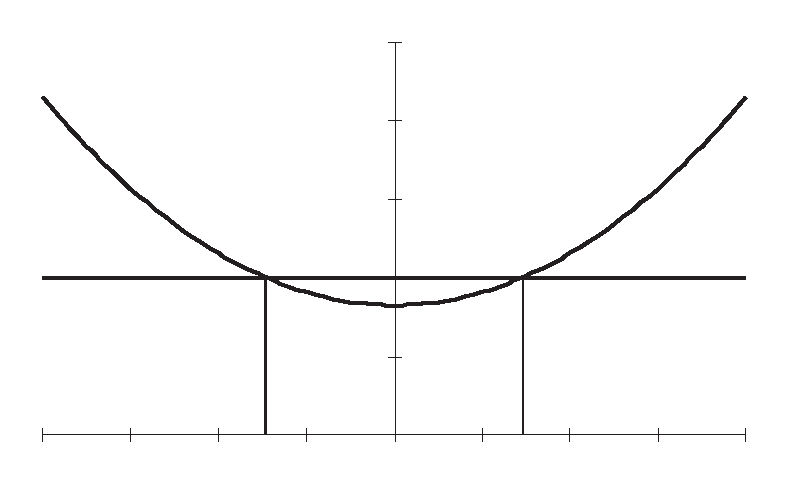
\includegraphics{./imatges/compara-riscs2.eps}
%\includegraphics[width=8cm]{./imatges/compara-riscs.eps}
\caption{Comparaci� del risc de dos estimadors}
\end{figure}
\end{example}

\begin{example}
Un exemple trivial for�a interessant �s el
seg�ent. Per estimar un par�metre $\theta$ l'estimador que
consisteix en un valor fix $\theta_0$, t� risc $0$ en
$\theta=\theta_0$. El risc, per�, augmenta molt a mida que ens
allunyem del valor real de $\theta$. De forma que no resulta un
estimador raonable, tot i que el seu risc pugui ser m�nim per
algun (un) valor de $\theta$.
\end{example}

Els exemples anterior ens mostren que els criteris de prefer�ncia
entre estimadors basats en el risc o en l'EQM no s�n de gran
utilitat general ja que molts estimadors poden ser incomparables.
Davant d'aquest fet ens plantegem si �s possible completar el
criteri de minimitzar el risc mitjan�ant alguna propietat o
criteri addicional. Les possibles solucions obtingudes a aquesta
q�esti� passen per dues vies:
\begin{enumerate}
\item  Restringir la classe dels estimadors considerats a aquells que
compleixin alguna propietat addicional d'inter�s, tot seleccionant
aquells de forma que s'eliminen els estimadors indesitjables i que
el criteri de minimitzar el risc permeti seleccionar-ne un
preferible a la resta. Aquest criteri ens duu a considerar les
propietats desitjables dels estimadors com \emph{manca de biaix,
consist�ncia, efici�ncia} i a analitzar com combinar-los amb el
criteri del m�nim risc. El proc�s culmina amb l'estudi dels
\emph{Estimadors Sense biaix Uniformement de M�nima Vari�ncia
(ESUMV)}.
\item  Refor�ar el criteri de prefer�ncia d'estimadors pel
procediment de reduir tota la funci� de risc $R_T(\theta)$ a un
�nic nombre representatiu que permeti ordenar linealment tots els
estimadors. Aquest criteri ens duu als \emph{Estimadors Bayes} i als
\emph{Estimadors Minimax}.
\end{enumerate}
\clearpage

\section{Estudi de les propietats desitjables dels estimadors}

\subsection{El biaix}
Suposem que tenim un model estad�stic $\modest$ i un estimador
$T(\Sample)$ d'una funci� mesurable $g(\theta)$ del par�metre. Una
forma raonable de valorar qu� tan pr�xims s�n els valors de $T$
dels de g($\theta )$ �s veure si, en promig, els valors de $T$
coincideixen amb el valor mitj� de g($\theta )$.
\begin{definition}
Sota les condicions esmentades, si $E_\theta (T)$ �s l'esperan�a
de $T(\Sample)$ i $g(\theta)$ �s una funci� del par�metre (en
particular la identitat) la difer�ncia
\[
\bias=b_T(\theta)=E_\theta (T)-g(\theta )
\]
rep el nom de \emph{biaix de l'estimador $T$ per estimar $g(\theta
)$}. \par
Si el biaix �s nul, �s a dir si:
\[
E_\theta (T)=g(\theta ),\quad \forall\, \theta \in \Theta
\]
direm que $T$ �s un estimador \emph{no esbiaixat de }$g(\theta)$.
\end{definition}

\begin{example}
Els dos exemples m�s coneguts s�n el del la mitjana i la
vari�ncia mostrals.
\begin{itemize}
\item  La mitjana mostral �s un estimador sense biaix de $\mu$.
\item  La vari�ncia mostral �s un estimador amb biaix de la
vari�ncia poblacional. En concret el seu biaix val:
$$
b_{s^2}(\sigma^2)=E_{\sigma^2}(s^2)-\sigma^2=
\frac{n-1}n\,\sigma ^2-\sigma^2=\frac{-1}n\sigma ^2
$$
\end{itemize}
\end{example}

L'�s d'estimadors sense biaix �s convenient en mostres de mida
gran. En aquestes $\mathrm{var}_\theta(T) $ �s sovint
petita i aleshores, com $E_\theta (T) =g(\theta) +b_T(\theta)$, �s
molt probable obtenir estimacions centrades en aquest valor en
lloc de l'entorn $g(\theta)$.
\begin{example}
Sigui $\Sample$ una mostra aleat�ria simple de $X\sim
U(0,\theta)$. Agafem $T=\max\{\Sample\}$ com l'estimador del m�xim
de la distribuci�. �bviament podem dir que $T<\theta$ i per tant
l'estimaci� �s sempre esbiaixada. Com hem vist en l'exemple
\ref{Exemple-Risc-1}, la distribuci� en el mostratge de $T$ �s
\[
H_\theta ( t) =P_\theta \left[ T\leq t\right] =\left(\frac
t\theta\right)^n
\]
i la seva funci� de densitat �s
\[
f_\theta ( \theta ) =H_\theta ^{\prime }( \theta ) =\frac n\theta
\left( \frac t\theta \right) ^{n-1}
\]
La seva esperan�a (veure exemple \ref{Exemple-Risc-1}) val
\[
E_\theta ( T) =\int_0^\theta t\cdot \left[ \frac n\theta \left(
\frac t\theta \right) ^{n-1}\right] dt=\frac n{n+1}\theta
\]
d'on el biaix de $T$ per estimar $\theta $ �s
\[
b_T(\theta) =\frac n{n+1}\,\theta -\theta =-\frac 1{n+1}\,\theta
\]
\end{example}

Podem preguntar-nos sin� podr�em millorar aquest estimador tot
corregint el biaix de forma an�loga al que f�iem amb $\hat{s}^2$,
�s a dir, agafar un estimador \emph{corregit per al biaix}
$$
T^{\prime}=\frac{n+1}n\,T\quad \text{que, per construcci�,
verifica: } E(T^{\prime})=\theta.
$$
Considerem l'estimador de m�nim risc en el sentit de l'error
quadr�tic mitj�, �s a dir, l'estimador que minimitza $E\left[ (
\theta -T) ^2\right]$. De fet, com hem vist en l'exemple
\ref{Exemple-Risc-1} conv� escollir el que minimitza
$E[(\theta-T)^2/\theta^2]$, perqu� tamb� minimitza l'EQM per�
assoleix un m�nim absolut. Aquest estimador �s
\[
T''=\frac{n+2}{n+1}\,T
\]
i per tant �s m�s adient que $T^{\prime}$, ja que t� un menor risc
respecte de l'error quadr�tic mitj�.

Quan, com aqu�, ens trobem que donat un estimador en podem trobar
un de menor risc, diem que el primer no �s admissible respecte de
la funci� de p�rdua. En aquest cas diem que $T'$ no �s admissible
respecte l'EQM. Compte! aix� no vol dir que no el puguem fer
servir sin� que n'hi ha un amb menys risc, ja que existeix un
altre $T''$ preferible a ell que, per cert, no �s centrat.
Efectivament
\[
E_\theta (T'') =\frac{n+2}{n+1}\,E_\theta (T)
=\frac{(n+2)n}{(n+1)^2}\,\theta
\]

L'exemple anterior mostra que degut a la descomposici�
$EQM_T( \theta ) =\mathrm{var}_\theta(T)+b_T^2(\theta)$ pot ser
preferible un estimador amb biaix a un altre que no en t�.

En general, per�, e{\ll}iminar el biaix no �s una mala estrat�gia,
sobretot pel fet que al restringir-nos a la classe dels
estimadors sense biaix obtenim una soluci� constructiva que
permetr� obtenir estimadors sense biaix de m�nima vari�ncia en
condicions bastant generals.

Els exemples seg�ents i{\ll}ustren dues propietats interessants del
biaix. D'una banda mostren que no sempre existeix un estimador sense
biaix. D'altra veiem com de vegades, tot i tenir un
estimador sense biaix per a un par�metre $E_\theta (T) =\theta$,
una funci� $g(T) $ no �s necess�riament un estimador sense biaix
de $g(\theta)$.
\begin{example}
Considerem una variable $X$ amb distribuci� de Bernouilli $B(1,p)$.
Suposem que desitgem estimar $g(p)=p^2$ amb una �nica observaci�.
Per tal que un estimador
$T$ no tingui biaix per estimar $p^2$ caldria que
$$
p^2=E_p(T)=p\cdot T(1)+(1-p)\cdot T(0),\quad 0\leq p\leq 1
$$
�s a dir, per a qualsevol valor de $p\in[0,1]$ s'hauria de
verificar
$$
p^2=p\cdot (T(1)-T(0))+ T(0)
$$
Aix� no �s clarament possible, ja que l'�nica forma que
una funci� lineal i una funci� parab�lica coincideixin en tot
l'interval $[0,1]$ �s quan els coeficients $T(0)$ i $T(1)$
valen zero.
\end{example}
\begin{example}
El par�metre $\alpha$ d'una llei exponencial amb funci� de
densitat
$$f(x)=\alpha \,e^{-\alpha x}\,\mathbf{1}_{(0,\infty)}(x)
$$
�s l'invers de la mitjana de la distribuci�, �s a dir
$\alpha =1/EX$.

Un estimador raonable de $\alpha =g(\mu)$ pot ser $\hat{\alpha}=g(\hat{\mu})$,
�s a dir $\hat{\alpha}=1/\bar{X}$.
Si apliquem la propietat de que la suma de variables aleat�ries
i.i.d. exponencials segueix una llei gamma de par�metres
$n$ i $\alpha$, s'obt� que aquest estimador t� biaix. La
seva esperan�a �s
\[
E(\hat{\alpha})=\frac n{n-1}\,\alpha
\]
El biaix es corregeix simplement amb
$$\hat{\alpha}^{\prime}=\frac{n-1}n \,\hat{\alpha}$$
\end{example}

\subsection{Consist�ncia}

La consist�ncia d'un estimador �s una propietat for�a intu�tiva
que ve a dir, informalment, que quan augmenta la mida
mostral el valor de l'estimador s'acosta cada cop m�s a
l'aut�ntic valor del par�metre.
\begin{definition}
Sigui $\Sample,\dots$ una successi� de variables aleat�\-ries i.i.d. $X\sim
F_\theta$, $\theta \in \Theta$. Una successi� d'estimadors
puntuals $T_n=T(\Sample)$ s'anomena consistent per $g(\theta)$
si $$T_n\stackunder{n\rightarrow
\infty }{\stackrel{P}{\longrightarrow }}g(\theta)$$ per a cada
$\theta \in \Theta$, �s a dir si
\[
\forall \varepsilon >0 \qquad
\lim_{n\to\infty}P\left\{ \left| T_n-g( \theta ) \right| >\varepsilon
\right\}=0
\]
\end{definition}

Observem que:
\begin{enumerate}
\item  Es tracta d'un concepte asimpt�tic: Parlem de ``successions
d'estimadors consistents'' m�s que d'estimadors
pr�piament dits.
\item  La definici� es pot refor�ar si, en lloc de considerar
converg�ncia en probabilitat (consist�ncia feble), considerem converg�ncia
quasi segura o en mitjana quadr�tica:
\begin{itemize}
\item  $T_n$ �s fortament consistent si
$T_n\,{\stackrel{\textrm{q.s.}}{\longrightarrow }}\,g( \theta )$
\item  $T_n$ �s consistent en mitjana-$r$ si $E_\theta \left[ \left|
T_n-g( \theta ) \right| ^r\right] \longrightarrow 0$
\end{itemize}
\end{enumerate}
\begin{example}
Molts estimadors consistents ho s�n com a conseq��ncia de les lleis
dels grans nombres. Recordem que la Llei feble dels Grans Nombres
(Txebytxev) afirma que donada una successi� de v.a.~independents i
id�nticament distribu�des amb mitjanes $\mu<\infty$ i vari�ncies
$\sigma^2<\infty $ llavors
$$\bar{X}_n\stackrel{P}{\longrightarrow }\mu$$
Com a conseq��ncia d'aquesta llei i at�s que una mostra
aleat�ria simple �s i.i.d., per definici�, podem afirmar que
$\bar{X}_n$ �s consistent per estimar $\mu$.
\end{example}

\begin{example}\label{Ex-Consistencia-Maxim}
La succesi� $T_n=\max_{1\leq i\leq n}\{ X_i\}$ �s consistent per estimar el m�xim
d'una distribuci� uniforme en $[0,\theta]$:
\[
P\left[\left| \stackunder{1\leq i\leq n}{\max}\{ X_i\}-\theta
\right| >\varepsilon \right] =P\left[ \theta -\stackunder{1\leq i\leq n}{%
\max}\{X_i\}>\varepsilon \right]
\]
ja que $X_i\in [0,\theta]$ i, per tant, podem escriure:
\[
\begin{split}
P\left[ \theta -\varepsilon >\stackunder{1\leq i\leq n}{\max
}\{X_i\}\right] &=P\left[\stackunder{1\leq i\leq n}{\max
}\{X_i\}<\theta -\varepsilon \right]  \\
&=\left( \frac{\theta -\varepsilon }\theta \right) ^n= \left (
1-\frac \varepsilon \theta \right) ^n \stackunder{n\rightarrow
\infty }{\longrightarrow }0
\end{split}
\]
�s immediat comprovar que
$$
E\left[ ( \theta -T_n) ^2\right]
=\left( 1-\frac{2n}{n+1}+\frac n{n+2}\right)\,\theta ^2
$$
que tamb� tendeix a zero quan $n\to\infty$ i per tant
$T_n= \max_{1\leq i\leq n}\{X_i\}$ tamb� �s consistent
en mitjana quadr�tica.
\end{example}

Normalment, quan es parla de consist�ncia es fa refer�ncia a la
converg�ncia en probabilitat, �s a dir, $T_n$ �s consistent si
$\lim_{n\to\infty}P(| T_n-g(\theta )| >\varepsilon)=0$. Si
l'estimador no t� biaix, estem en la situaci� d'aplicar la
desigualtat de Txebytxev\footnote{Si $\mathrm{var}(X)$ existeix, aleshores
$\forall \varepsilon >0$ es verifica $P(| X-E(X)| >
\varepsilon) \leq \frac{ \mathrm{var}(X)}{\varepsilon^2}$}:

Si $E( T_n)=g(\theta ) $, aleshores
\[
P( \left| T_n-g( \theta ) \right| >\varepsilon )
=P( \left| T_n-E( T_n) \right| > \varepsilon) \stackunder{\textrm{Txebytxev}}{\leq}
\frac{\mathrm{var}(T_n)}{\varepsilon^2}
\]
Aix�, per mirar d'establir la consist�ncia de $T$ hem de
provar que
$$\frac{\mathrm{var}(T_n)}{\varepsilon^2} \tendsto 0$$
\begin{example}
Sigui $M_n=\sum_{i=1}^n a_iX_i$ una combinaci�
lineal dels valors de la mostra amb coeficients tals que
$\sum_{i=1}^n a_i=1$ i algun $a_i>0$. �s consistent $M_n$ per
estimar $E(X)$?

Comencem per veure que $M_n$ no t� biaix
\[
\begin{split}
E( M_n) &=E\left ( \sum_{i=1}^n a_iX_i\right ) =\sum_{i=1}^n
E(a_i X_i) \\
&=\sum_{i=1}^n a_iE(X_i) \stackrel{i.i.d.}{=}\sum_{i=1}^n
a_iE(X)=E(X)
\end{split}
\]
Calculem la vari�ncia
\[
\begin{split}
\mathrm{var}(M_n) &= \mathrm{var}\left(\sum_{i=1}^n a_iX_i\right)
=\sum_{i=1}^n \mathrm{var}( a_iX_i) \\
&=\sum_{i=1}^n a_i^2\mathrm{var}( X_i)=\mathrm{var}(X)
\sum_{i=1}^n a_i^2
\end{split}
\]

Si apliquem ara la desigualtat
de Txebytxev tenim:
\[
P( \left| M_n-\mu \right| >\varepsilon ) \leq \frac{\sigma ^2\sum
a_i^2}{\varepsilon ^2}
\]
que no t� perqu� tendir a 0 quan $n\to\infty$ i, per tant, no
podem afirmar que l'estimador �s consistent. Per exemple, si
$a_1=\frac 12,a_2=a_3=\dots=a_n=\frac 1{2(n-1)}$ tindrem que
$\lim_{n\to\infty}\sum a_i^2= \frac 14$.\par Observem que el
resultat obtingut no pot assegurar la consist�ncia de $M_n$ per a
qualsevol fam�lia de coeficients $a_1,\dots,a_n$, per� �bviament
l'estimador �s consistent per a alguna (cas $a_i=1/n$).
\end{example}

\begin{example}
Tornem a l'exemple de l'estimador de $EX$ d'una distribuci�
exponencial $f(x)=\alpha \cdot \exp \{-\alpha\,x\}\cdot
\mathbf{1}_{(0,\infty )}(x)$ que hem vist al parlar del biaix. Si
considerem l'estimador
\[
\hat{\alpha}= 1/\bar{X}
\]
podem, un cop m�s tot aplicant les propietats de la llei gamma de
par�metres $n$ i $\alpha$, obtenir la seva vari�ncia
\[
\mathrm{var}(\hat{\alpha})=\frac 1{(n-1)^2(n-2)}\alpha^2
\]
En conseq��ncia, la vari�ncia de l'estimador corregit per al biaix
$\hat{\alpha}^{\prime}=\frac{n-1}n\hat{\alpha}$ val
\[
\begin{split}
\mathrm{var}(\hat{\alpha}^{\prime})
&=\left(\frac{n-1}n\right)^2\mathrm{var}(\hat{\alpha})
=\left(\frac{n-1}n\right)^2\frac 1{(n-1)^2(n-2)}\,\alpha ^2 \\
&=\frac 1{n^2(n-2)}\,\alpha ^2
\end{split}
\]
Aix� resulta obvi que, si apliquem la desigualtat de Txebytxev
obtindrem que l'estimador $\hat{\alpha}^{\prime}$ �s
consistent. Per tant, tamb� ho �s $\hat{\alpha}$ que
coincideix amb aquest quan $n$ tendeix a infinit.
\end{example}

\subsubsection{Propietats dels estimadors consistents}

Moltes de les propietats dels estimadors s�n conseq��ncia directa
de les propietats de la converg�ncia en probabilitat, que podeu
revisar per exemple a Martin Pliego (1998a) cap�tol 11.

\begin{enumerate}
\item  Si $T_n$ �s consistent per estimar $\theta\,$ i
$g:\Real\rightarrow\Real $ �s una funci� cont�nua, aleshores
$g(T_n)$ �s consistent per estimar $g(\theta)$.

\item  Si $T_{1n}$ i $T_{2n}$ s�n
consistents per estimar $\theta_1$ i $\theta_2$ respectivament, aleshores
\begin{description}
\item  $aT_{1n}\pm bT_{2n}$ �s
consistent per estimar $a\theta_1\pm b\theta_2$
\item  $T_{1n}\cdot T_{2n}$ �s
consistent per estimar $\theta_1\cdot \theta_2$
\item  $T_{1n}/T_{2n}$ �s consistent per estimar $\theta_1/\theta_2$,
si $\theta_2\neq 0$.
\end{description}
\item  Sigui $a_r=(1/n)\sum X_i^r$ el moment mostral d'ordre $r$.
Com s'ha vist al cap�tol 1, l'esperan�a de $a_r$ �s
\[
E(a_r) =E\left [ \frac 1n\sum X_i^r\right]
=\frac 1n\sum E(X^r)=\frac 1n n\alpha _r=\alpha _r
\]
on $\alpha_r$ �s el moment poblacional d'ordre $r$. Aix� doncs,
$a_r$ no t� biaix per estimar $\alpha_r$. La seva
vari�ncia �s
\[
\begin{split}
\mathrm{var}(a_r)&=\mathrm{var}\left(\frac 1n\sum X_i^r\right)
=\frac 1{n^2}\sum \mathrm{var}(X^r)
=\frac 1nE\left[ X^r-E( X^r) \right]^2 \\
&=\frac 1nE\left[X^r-\alpha _r\right] ^2 =\frac 1nE(
X^{2r}+\alpha _r^2-2\alpha _rX^r)\\
&= \frac 1n(\alpha_{2r}-\alpha _r^2).
\end{split}
\]
Y si apliquem la desigualtat de Txebytxev s'obt�
\[
P\left(|a_r-\alpha_r|\geq\varepsilon \right) \leq
\frac{E(a_r-\alpha_r)^2}{\varepsilon^2}=
\frac{\mathrm{var}(a_r)}{\varepsilon^2}=
\frac{\alpha_{2r}-\alpha_r^2}{n\varepsilon^2}\tendsto 0
\]
Aix� doncs, em vist que els moments mostrals s�n estimadors
consistents dels moments poblacionals.
\end{enumerate}

\subsection{Estimadors eficients}

Com ja hem vist, un objectiu desitjable en la cerca d'estimadors
optims �s considerar estimadors de ``m�nim risc'' o, si ens basem en la
funci� de p�rdua quadr�tica, estimadors que minimitzin l'error
quadr�tic mitj� $E(\theta-T)^2$.

En general �s dif�cil trobar estimadors que facin m�nim l'EQM per
a tots els valors de $\theta$ per�, si ens restringim als estimadors
sense biaix, el problema t� soluci� en un ventall m�s ample de
situacions.

Suposem que $T_1,T_2$ s�n dos estimadors sense biaix d'un
par�metre $\theta$. Per a aquests estimadors tenim que
\[
\begin{split}
EQM_{T_1}(\theta) &=\mathrm{var}_\theta (T_1)
+b^2_{T_1}(\theta) \\
EQM_{T_2}(\theta) &= \mathrm{var}_\theta (T_2) +
b^2_{T_2}(\theta )
\end{split}
\]
Si els estimadors no tenen biaix $b_{T_1}(\theta) =b_{T_2}(\theta)=0$
i el que tingui menys vari�ncia tindr� el risc menor
per estimar $\theta$. Si, per exemple,
$\mathrm{var}(T_1)\leq\mathrm{var}(T_2)$
direm que $T_1$ �s m�s eficient que $T_2$ per estimar
$\theta$.
\begin{figure}
\centering
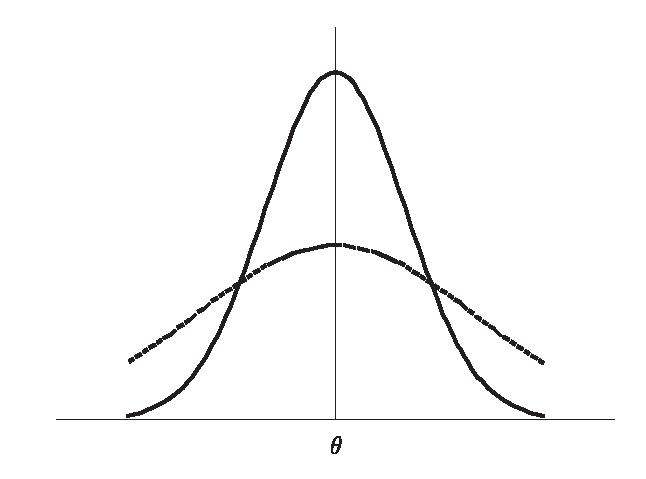
\includegraphics{./imatges/eficienc3.eps}
\caption{Comparaci� de l'efici�ncia de dos estimadors per a un $\theta$ donat}
\end{figure}

Per a dos estimadors amb biaix zero $b_{T_i}(\theta)=0$, el quocient
\[
ER=\frac{EQM_{T_1}(\theta)}{EQM_{T_2}(\theta)}
=\frac{\mathrm{var}_{\theta}(T_1)}{\mathrm{var}_{\theta}(T_2)}
\]
s'anomena \emph{efici�ncia relativa de $T_1$ respecte
$T_2$}. Si nom�s hi ha dos estimadors de $\theta$ pot ser
f�cil veure quin �s el m�s eficient. Si n'hi ha m�s, la cosa es
complica. El ``m�s eficient'', cas de que existeixi, s'anomenar�
\emph{l'estimador sense biaix de m�nima vari�ncia}.
\begin{definition}
Sigui $\mathcal{S}(\theta)$ la classe dels estimadors sense biaix de
$\theta$ i amb vari�ncia. Si per a tots els estimadors d'aquesta classe
$T\in \mathcal{S}(\theta)$ es verifica que
\[
\mathrm{var}_\theta(T)\leq\mathrm{var}_\theta(T^{\ast})
\quad \forall T\in\mathcal{S}(\theta)
\]
direm que $T^{\ast}$ �s un estimador sense biaix de m�nima vari�ncia de
$\theta$. Si la desigualtat �s certa $\forall \theta \in \Theta$
direm que $T^{\ast}$ �s un \emph{estimador sense biaix uniforme de
m�nima vari�ncia} ESUMV\footnote{UMVUE, en angl�s}.
\end{definition}

\subsection{Informaci� de Fisher i cota de Cramer-Rao}

�bviament, en un problema d'estimaci� l'ideal �s disposar d'un
ESUMV, per� aix� no sempre �s possible. Se'ns plantegen diversos
problemes:
\begin{enumerate}
\item  Existeixen ESUMV per a un par�metre $\theta$ en un model donat?
\item  En cas que existeixi l'ESUMV, sabrem com trobar-ho?
\end{enumerate}
Aquest problema t� soluci�, sota certes condicions, fent
servir els teoremes de Lehmann-Scheff� i Rao-Blackwell i el
concepte de sufici�ncia, que es discuteix m�s endavant.

Una soluci� parcial apareix gr�cies al \emph{Teorema de
Cramer-Rao} que permet establir una cota m�nima per a la vari�ncia
d'un estimador. Quan un estimador assoleixi aquesta cota sabrem
que �s un estimador de vari�ncia m�nima.

Informalment aquest resultat ve a dir que, sota certes condicions
de regularitat, si $T$ �s un estimador sense biaix d'un par�metre
$\theta$, la seva vari�ncia est� acotada per una expressi� que
anomenen \emph{cota de Cramer-Rao} $\mathrm{CCR}(\theta)$
\[
\mathrm{var}(T) \geq \mathrm{CCR}(\theta)
\]
Abans d'establir amb precisi� aquest teorema anem a considerar el
concepte d'informaci� d'un model estad�stic introdu�t per Fisher.
%\footnote{Els raonaments relatius a la cota de Cramer-Rao es poden
%seguir independentment de quant clar quedi el perqu� $I_n(\theta)$
%�s una mesura d'informaci�. Per aquest motiu la justificaci� de
%$I_n(\theta)$ com a mesura d'informaci� es rel.lega a l'ap�ndix
%del final del cap�tol}.

\subsubsection{Informaci� i versemblan�a d'un model estad�stic}
\label{Informacio-i-versemblansa}
Una idea bastant raonable �s
esperar que un estimador funcioni millor en el seu intent
d'aproximar-se al valor d'un par�metre quanta m�s informaci�
tingui per fer-ho. Per aquest motiu la vari�ncia de l'estimador i
la informaci� es presenten com a quantitats oposades: a m�s
informaci�, menys error (vari�ncia) en l'estimaci�:
\[
\mathrm{var}( \te_n) \propto \frac 1{I_n( \theta ) }
\]
Ara ens trobem amb el problema de \emph{com} definir la quantitat
d'informaci� (continguda en una mostra/d'un model), per tal que
s'ajusti a la idea intu�tiva d'informaci�. Fisher ho va fer a
trav�s de la funci� de versemblan�a\footnote{``verosimilitud'' en
castell� i ``likelihood'' en angl�s}.

Sigui un model estad�stic $\modest$ i una m.a.s.~$(\Sample)$, que
pren valors $\bx=(\sample)$. Si $X$ �s discreta la funci� de massa
de probabilitat indica, a grans trets, la probabilitat d'observar
la mostra, donat un valor del par�metre. Si $X$ �s absolutament
cont�nua aquesta interpretaci� ja no �s tan directa.
\[
f(x_1,x_2,\dots,x_n;\theta ) =\left\{
\begin{array}{ll}
P_\theta [ X=x_1] \cdots P_\theta [X=x_n],&\textrm{si $X$ �s discreta}\\
f_\theta(x_1) \cdots f_\theta(x_n),&\textrm{si $X$ �s abs.
cont�nua}
\end{array}
\right.
\]
La funci� de versemblan�a s'obt� si considerem, en l'expressi�
anterior, que el que queda fixat �s la mostra i no el par�metre.
�s a dir, fixada una mostra $\bx$ la funci� de versemblan�a indica
\emph{com de versemblant resulta}, per a cada valor del par�metre,
que el model l'hagi generada.
\begin{example}
Suposem que tenim una m.a.s.~$\sample$ de mida $n$ d'una variable
aleat�ria $X$, que segueix una llei de Poisson de par�metre
$\lambda$ desconegut.
$$
X \sim F_\lambda =P( \lambda ),\ \lambda >0
$$
La funci� de probabilitat de la mostra, fixat $\lambda$, �s:
$$
g_\lambda(\sample)=\stackunder{i=1}{\stackrel{n}{\prod }}e^{-\lambda }\frac{\lambda
^{x_i}}{x_i!}=e^{-n\lambda }\frac{\lambda ^{\sum x_i}}{\stackunder{i=1}{%
\stackrel{n}{\prod }}x_i!}$$ i la funci� de versemblan�a del
model, fixada $\bx$, �s:
$$
L(\sample;\lambda ) =\stackunder{i=1}{\stackrel{n}{\prod
}}e^{-\lambda }\frac{\lambda
^{x_i}}{x_i!}=e^{-n\lambda }\frac{\lambda ^{\sum x_i}}{\stackunder{i=1}{%
\stackrel{n}{\prod }}x_i!}$$ Tot i que la forma funcional de
$g_\lambda(\bx)$ i $L(\bx; \lambda)$ �s la mateixa, el seu aspecte
�s ben diferent com es pot comprovar en la figura
~\ref{fig-likelihoods} on donem valors a $g_\lambda(\bx)$, fent
variar $\bx$ o a $L(\lambda; \bx)$ fent variar $\lambda$.
\end{example}
\begin{figure}
\includegraphics{./imatges/versemblanca1.eps}\\
\includegraphics{./imatges/versemblanca2.eps}
\caption{Probabilitat de la suma de $n=5$ valors mostrals
per a 10 mostres de la llei de Poisson amb $\lambda=3$ versus
la funci� versemblan�a per a una mostra observada.}
\label{fig-likelihoods}
\end{figure}

%\begin{figure}
%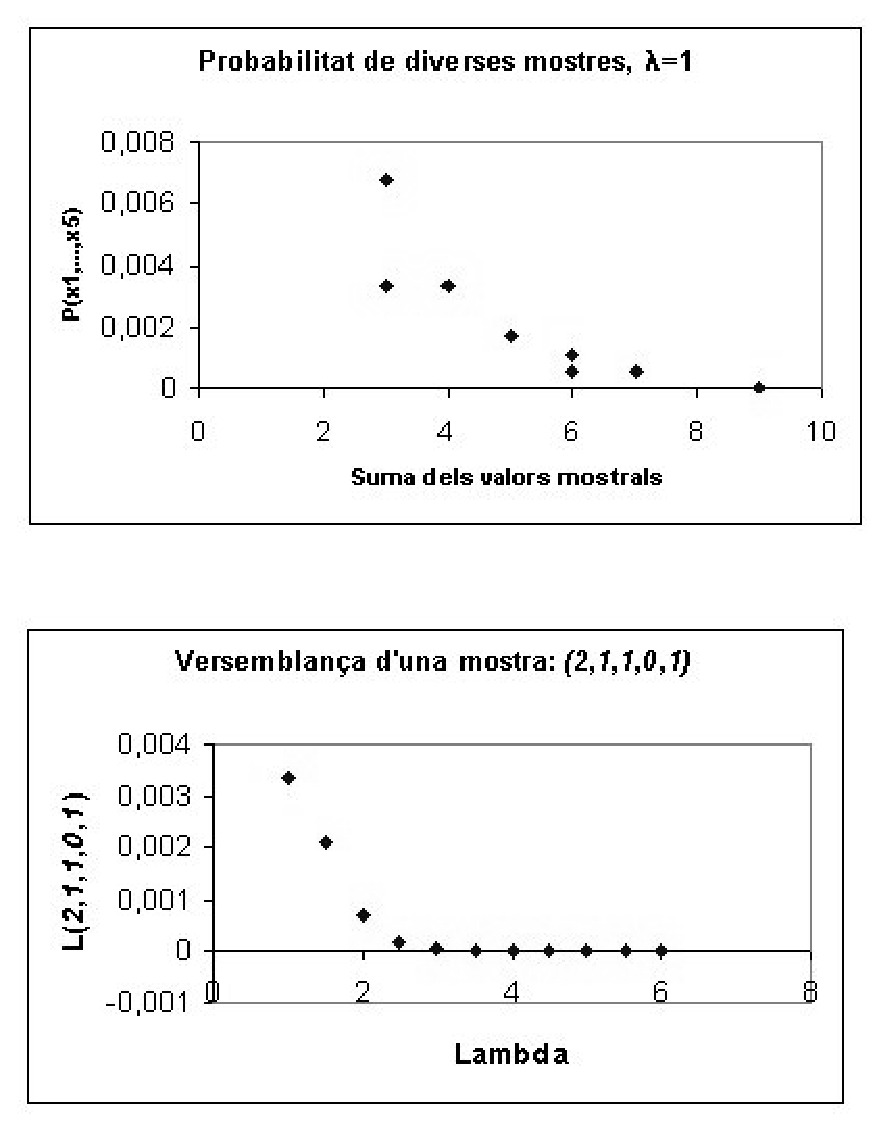
\includegraphics{./imatges/likelihood.eps}
%\caption{Probabilitat d'una mostra vs versemblan�a}
%\label{fig-likelihoods}
%\end{figure}

\subsubsection{Informaci� de Fisher}

Per tal de poder calcular la quantitat d'informaci� de Fisher que
hi ha continguda en una mostra sobre un par�metre, cal considerar
models estad�stics regulars, �s a dir, on es verifiquen les
seg�ents condicions de regularitat.

\begin{definition}
Direm que $\modest$ �s un model estad�stic regular si es
verifiquen les seg�ents condicions:
\begin{enumerate}
\item  La poblaci� d'on prov� la mostra presenta un ``camp de
variaci�'' o suport $S_{\theta}=\{ x|\, f( x;\theta)>0\}=S$ que no
dep�n de $\theta$.
\item  La funci� $L(\bx;\theta)$ admet, com a m�nim, les dues primeres derivades.
\item  Les operacions de derivaci� i integraci� s�n
intercanviables.
\end{enumerate}
\end{definition}

\begin{definition}
Sigui $\modest$ un model estad�stic regular, �s a dir, on es
verifiquen les condicions de regularitat 1-3 d'abans. Si
$Z=\frac\partial{\partial\theta}\log L(\bX;\theta)$, la quantitat
d'informaci� de Fisher �s
\[
I_n(\theta) =\mathrm{var}_\theta (Z)=\mathrm{var}_\theta \left(
\frac\partial{\partial\theta }\log L(\bX;\theta) \right)
\]
\end{definition}
Les condicions de regularitat s�n necess�ries per poder fer el
c�lcul de $E_\theta(Z^2)$.

\medskip
A continuaci� presentem algunes propietats de la
informaci� de Fisher. Podeu veure la demostraci� a Ruiz--Maya i
Pliego (1995).
\begin{enumerate}
\item La informaci� de Fisher es pot expressar com:
\[
I_n( \theta )=E_{\theta}\left[ \left(
\frac{\partial\log L(\bX;\theta)}{\partial\theta}
\right)^2\right]
\]
Aix� es pot comprovar, ja que si apliquem les condicions de regularitat
\[
\begin{split}
E(Z) &= E\left(
\frac{\partial\log L(\bX;\theta)}{\partial\theta}\right)
= \int_{S^n}
\frac{\partial\log L(\bx;\theta)}{\partial\theta}
L(\bx;\theta)\,d\bx\\
&= \int_{S^n}
\frac{\frac{\partial L(\bx;\theta)}{\partial\theta}}{L(
\bx;\theta)}L(\bx;\theta)\,d\bx
=\int_{S^n}\frac{\partial
L(\bx;\theta)}{\partial\theta}\,d\bx \\
&=\frac\partial {\partial\theta}\stackunder{%
=1}{\underbrace{\int_{S^n}L(\bx;\theta)}}\,d\bx=
\frac\partial{\partial\theta}\,1=0
\end{split}
\]
De forma que $E(Z)=0$ i per tant tindrem que
$\mathrm{var}_\theta (Z)=E_\theta(Z^2)$.
\item  $I_n(\theta)=0$ si i nom�s si $L(\bx;\theta)$
no dep�n de $\theta$.
\item  Donades dues m.a.s.~$\bx_1,\bx_2$ de mides $n_1,n_2$, de la
mateixa poblaci� es verifica:
\[
I_{n_1,n_2}(\theta) =I_{n_1}(\theta)+I_{n_2}(\theta)
\]
De manera que podem considerar una mostra de mida $n$ com $n$
mostres de mida $1$:
\[
I_n(\theta) =\sum_{i=1}^n I_1( \theta ) =n\cdot i( \theta ),
\text{ essent }i( \theta )=I_1( \theta )
\]
�s a dir
\[
E\left( \frac{\partial \log ( L(\bX;\theta))}{\partial \theta
}\right) =nE\left( \frac{\partial \log f(X;\theta)}{\partial
\theta }\right)
\]
\item  Es verifica la seg�ent relaci�:
\[
I_n(\theta) =E\left[ \left(\frac{\partial \log L(\bX;\theta)}
{\partial\theta}\right)^2\right] =-E\left[
\frac{\partial^2\log L(\bX;\theta) }{\partial^2\theta}\right]
\]
\end{enumerate}

\begin{example}
Anem a calcular la quantitat d'informaci� de Fisher continguda en
una m.a.s.~extreta d'una poblaci� $N(\mu,\sigma)$ amb $\sigma=\sigma_0
$ coneguda.\\ La funci� de versemblan�a �s
\[
L(\bx;\mu) =\stackunder{i=1}{\stackrel{n}{\prod}}%
\frac 1{\sqrt{2\pi}\sigma_0}
e^{-\frac{(x_i-\mu )^2}{2\sigma_0^2}}=
(2\pi\sigma_0^2)^{-n/2}\exp\left(-\sum_{i=1}^n
\frac{(x_i-\mu)^2}{2\sigma_0^2}\right)
\]
i el seu logaritme
\[
\log L(\bx;\mu) =-\frac n2\log(2\pi\sigma_0^2) -\frac
1{2\sigma_0^2}\sum_{i=1}^n (x_i-\mu)^2
\]
Si derivem respecte $\mu$
\[
\frac{\partial \log L(\bx;\mu)}{\mu} =-\frac
1{2\sigma _0^2}\,2\sum_{i=1}^n  ( x_i-\mu ) ( -1) =\frac{%
\sum_{i=1}^n ( x_i-\mu )}{\sigma_0^2}
\]
d'on
\[
\begin{split}
I_n(\mu)&=E\left(\frac{\partial\log L(\bX;\mu)}{\partial\mu}\right)^2
=E\left(\frac{\sum_{i=1}^n (X_i-\mu)}{\sigma_0^2}\right)^2 \\
&=\ \frac 1{\sigma_0^4}E\left[
\sum_{i=1}^n (X_i-\mu )^2 +\sum_{i\ne j} (X_i-\mu)(X_j-\mu) \right] \\
&=\frac 1{\sigma_0^4} E\left[ \sum_{i=1}^n (X_i-\mu)^2\right]+
\frac 1{\sigma_0^4}
\stackunder{=0}{\underbrace{E\left[\stackunder{i\neq
j}{\stackrel{n}{\sum }}( X_i-\mu ) (X_j-\mu)\right]}} \\
&=\frac 1{\sigma_0^4}\,n\sigma_0 ^2=\frac n{\sigma_0^2}
\end{split}
\]
Aquest c�lcul tamb� es pot fer a partir de la tercera
propietat de la informaci� de Fisher
\[
I_n(\mu)=nE \left[ \frac{\partial \log f(X;\mu)}{\partial\mu}\right]
=n \frac 1{\sigma_0^2} =\frac n{\sigma_0^2}
\]
\end{example}

\subsubsection{La desigualtat de Cramer--Rao}
Un cop establertes les condicions de regularitat i
caracter�stiques anteriors podem enunciar el teorema de
Cramer--Rao (1945).
\begin{theorem}
Donat un model estad�stic regular $\modest$, �s a dir, un model on
es verifiquen les condicions de regularitat enunciades, qualsevol
estimador $T\in\mathcal{S}(\theta)$ de la classe dels estimadors
no esbiaixats i amb vari�ncia verifica
\[
\mathrm{var}_\theta(T) \geq \frac 1{I_n(\theta)}
\]
\end{theorem}

\emph{Demostraci�:}
\par\medskip
L'estimador $T\in\mathcal{S}(\theta)$ no t� biaix, �s a dir que
\[
E(T) =\int_{S^n} T(\bx)\cdot L(\bx;\theta)\,d\bx =\theta
\]
Si derivem i introdu�m la derivada sota el signe de la integral, obtenim
\[
\begin{split}
\frac\partial{\partial\theta }E(T)
&=\int_{S^n} \frac\partial{\partial\theta}\left(T(\bx)\cdot L(\bx;\theta)\right)\,d\bx
=\int_{S^n} T(\bx) \frac\partial{\partial\theta}L(\bx;\theta)\,d\bx\\
&=\int_{S^n} T(\bx) \left(\frac{\frac\partial{\partial\theta}
L(\bx;\theta)}{L(\bx;\theta)}\right)L(\bx;\theta)\,d\bx
\end{split}
\]
%%Si de $t( \bx) $ en diem $\te_n$ i de $%
%( \frac{\frac \partial {\partial \theta }f( \bx;\theta
%) }{f( \bx;\theta ) }) $ en diem $Z$,
Aix� doncs
\[
1=\frac\partial{\partial\theta}\,\theta=\frac\partial{\partial\theta}E(T)
=E(TZ) =\int_{S^n} T(\bx)\cdot Z\,L(\bx;\theta)\,d\bx
\]
En resum
\[
E(T)=\theta,\ E(TZ)=1,\ E(Z)=0,\ \mathrm{var}(Z)=I_n(\theta)
\]
Si ara considerem el coeficient de correlaci� al quadrat entre
$T$ i $Z$, tenim
\[
\rho^2(T,Z) =
\frac{\left[\mathrm{cov}(T,Z)\right]^2}{\mathrm{var}(T)\cdot\mathrm{var}(Z)}
=\frac{\left[E(TZ)-E(T) E(Z)\right]^2}%
{\mathrm{var}(T) \cdot \mathrm{var}(Z) }\leq 1
\]
Si substitu�m els resultats trobats abans obtenim
\[
\frac 1{\mathrm{var}(T) \cdot I_n(\theta)}\leq 1
\]
d'on es dedueix la desigualtat enunciada.\hfill $\blacksquare$

\medskip
\begin{definition}
Si un estimador assoleix la CCR (Cota de Cramer--Rao) diem que �s
un \emph{estimador eficient}.
\end{definition}
Tot estimador eficient �s de m�nima vari�ncia en la classe
$\mathcal{S}(\theta)$. Per� tamb� pot passar que existeixi un
estimador de m�nima vari�ncia sense arribar necess�riament a la
CCR.
\begin{example}
Sigui $X\sim F_\theta =P(\lambda)$, $\lambda >0$ (Poisson).
Busquem la CCR dels estimadors de $\lambda$.
\[
\begin{split}
L(\bx;\lambda) &=\stackunder{i=1}{\stackrel{n}{\prod
}}e^{-\lambda }\frac{\lambda
^{x_i}}{x_i!}=e^{-n\lambda }\frac{\lambda ^{\sum x_i}}{\stackunder{i=1}{%
\stackrel{n}{\prod }}x_i!} \\
\log L(\bx;\lambda)  &=-n\lambda +\left(\sum
x_i\right)\log\lambda -\log\left(\stackunder{i=1}{\stackrel{n}{%
\prod }}x_i!\right)\\
\frac{\partial \log ( L(\bx;\lambda))}{%
\partial \lambda }&= -n+\left(\sum x_i\right)\frac 1\lambda\\
E\left[ \frac{\partial \log
L(\bx;\lambda)}{\partial\lambda}\right]^2 &= E\left[ n^2+\left(
\frac{\sum X_i}\lambda \right)^2-\frac{2n\sum
X_i}\lambda \right] \\
&= n^2+\frac 1{\lambda ^2}E\left(\sum
X_i\right)^2-\frac{2n}\lambda n E(X)
\end{split}
\]
En aquest punt, podem recordar que la suma de variables de Poisson
tamb� �s una Poisson
$$\sum X_i\sim P(n\lambda)$$
i per tant
\[
E\left(\sum X_i\right)^2 =\mathrm{var}( \sum X_i) +\left[
E\left( \sum X_i\right)\right]^2 =n\lambda  +( n\lambda ) ^2
\]
De forma que
$$
E(Z^2)= n^2+\frac 1{\lambda ^2}(n\lambda +n^2\lambda ^2) -%
\frac{2n^2\lambda }\lambda = n^2+\frac{n\lambda }{\lambda ^2}+\frac{n^2\lambda ^2}{\lambda ^2}%
-2n^2=\frac n\lambda
$$
i definitivament
$$
I_n(\lambda) =\frac n\lambda \quad\Longrightarrow\quad
\mathrm{var}(T) \geq \frac\lambda{n}
$$
Sabem que la mitjana aritm�tica verifica
$$\mathrm{var}(\bar{X}_n) =\frac \lambda{n}$$
de forma que coincideix amb la cota de Cramer--Rao i resulta que
$\bar{X}_n$ �s l'estimador eficient de $\lambda$.
\end{example}

\begin{example}
Per poder calcular la CCR o, m�s ben dit, per a que l'invers de
$$
E\left[\frac{\partial\log L(\bx;\theta)}{\partial\theta}\right]^2
$$
sigui de deb� la cota m�nima de
$\mathrm{var}(\widehat{\theta})$ dins la classe $\mathcal{S}(\theta)$
cal que es verifiquin les
condicions de regularitat. En cas contrari podem obtenir
resultats absurds.

Considerem, per exemple, una variable aleat�ria $X$
amb funci� de densitat
\[
f(x;\theta) =\frac 3{\theta ^3}x^2\mathbf{1}_{[0,\theta]}(x)
\]
i esperan�a
\[
E(X) =\int_0^\theta x\cdot\frac 3{\theta ^3} x^2\,dx
=\left.\frac 3{\theta^3}\frac{x^4}4\right|_0^\theta
=\frac 3{\theta^3}\frac{\theta^4}4=\frac 34\,\theta
\]
Com que $\theta =\frac 43E( X) $,
aix� suggereix estimar $\theta$ per $\widehat{\theta}=\frac 43\bar{X}$
que no t� biaix.

D'altra banda, si
calculem la vari�ncia de $X$ tenim
\[
\mathrm{var}(X)=E(X^2)-E(X)^2
=\int_0^\theta \frac 3{\theta^3}x^4\,dx-\left(\frac 34\,\theta\right)^2
=\frac 35\,\theta
^2-\frac 9{16}\,\theta^2=\frac{3}{80}\,\theta^2
\]
Ja sabem que $E(\widehat{\theta})=\theta$ i, a m�s,
\[
\mathrm{var}(\widehat{\theta}) =\mathrm{var}(\frac 43\bar{X})=%
\frac{16}9\mathrm{var}(\bar{X}) =\frac{16}9\frac{\mathrm{var}(X)}n
=\frac{16}9\frac 3{80}\frac{\theta^2}n=\frac{\theta^2}{15n}
\]

Si avaluem $I_n(\theta)$ en la forma m�s simple obtenim
\[
I_n(\theta) =nI(\theta)
=nE\left[ \frac{\partial \log f(X;\theta)}{\partial
\theta }\right]^2=n\frac 9{\theta^2}
\]
De forma que la CCR resulta ser m�s gran que la vari�ncia d'aquest
estimador
\[
\mathrm{var}(\widehat{\theta}) =\frac{\theta^2}{15n}<
\frac{\theta^2}{9n}
\]
la qual cosa �s absurda. L'absurd ha esdevingut
perqu� no hem tingut en compte que el suport de $X$ dep�n de
$\theta$ i les condicions de regularitat, en aquest cas, no es
verifiquen. La cota de Cramer--Rao no existeix.
\end{example}

Tamb� es dona el cas que la vari�ncia d'un estimador �s inferior a
la CCR encara que existeixi. Aix� pot passar, per exemple, per
algun estimador esbiaixat.

\subsubsection{Caracteritzaci� de l'estimador eficient}

Una cosa �s calcular la cota de Cramer--Rao i una altra �s trobar
l'estimador que assoleix aquesta cota i, en conseq��ncia, �s de
vari�ncia m�nima. La seg�ent caracteritzaci� permet, en algunes
ocasions, obtenir directament la forma de l'estimador eficient.

\begin{theorem}\label{Caracterizacio-Estimador-Eficient}
Sigui $T$ l'estimador eficient de $\theta$, aleshores es verifica
\[
\sum_{i=1}^n \frac\partial{\partial\theta}\log f(X_i;\theta)
=K(\theta,n) (T-\theta)
\]
on $K(\theta,n)$ �s una funci� que dep�n de $\theta$ i de $n$ i
que sol coincidir amb la informaci� de Fisher.
\end{theorem}

\emph{Demostraci�:}\par
Si $T$ �s l'estimador eficient, llavors
$$\mathrm{var}(T) =\frac 1{I_n(\theta)}$$
i per tant $\rho^2(T,Z)=1$.

En general, donades dues variables aleat�ries $X$ i $Y$ hom sap
que si $\rho(X,Y)=1$, aleshores
$$Y-E(Y)=\beta(X-E(X))$$
Si apliquem aquest resultat a $T$ i $Z$ tenim
\[
\begin{split}
Z-E(Z)&=\beta(T -E(T)) \\
\frac{\partial\log L(\bx;\theta)}{\partial\theta}-0
&=\beta(T -\theta) \\
\sum_{i=1}^n \frac{\partial\log f(X_i;\theta)}{\partial\theta}
&=K(\theta,n) (T-\theta)
\end{split}
\]


\begin{example}
En el cas de la distribuci� de Poisson tenim
\[
\begin{split}
f(x;\lambda) &= e^{-\lambda}\frac{\lambda^x}{x!}\\
\log  f(x;\lambda)  &= -\lambda
+x\log (\lambda) -\log (x!)\\
\frac{\partial\log f(x;\lambda)}{\partial\lambda}&=-1 +x\frac{1}{\lambda}
\\
Z=\sum_{i=1}^n \frac{\partial\log f(X_i;\lambda)}{\partial\lambda}
&=\sum_{i=1}^n \left(-1+\frac{X_i}\lambda\right)
\end{split}
\]
Volem veure que
$$
\sum_{i=1}^n \left( \frac{X_i}\lambda -1\right)
=K(\theta,n) (T-\theta)
$$
de forma que si ho re-escrivim adequadament
tenim
$$
\frac{1}{\lambda}\sum_{i=1}^n X_i -n=\frac 1\lambda
\left( \sum_{i=1}^n X_i-n\lambda \right) =\frac n\lambda \left(
\frac{1}{n}\sum_{i=1}^n X_i-\lambda\right)
$$
Aix� resulta que $K(\lambda,n)=n/\lambda$ i coincideix amb la
informaci� de Fisher $I_n(\lambda)$. Pel teorema
anterior es dedueix que $T=\bar{X}$ �s l'estimador eficient i, per tant,
de m�nima vari�ncia.
\end{example}

\subsubsection{CCR per a l'estimaci� d'una funci� param�trica}

Sigui $g$ una funci� real de variable real derivable i $V$ un
estimador sense biaix de $g(\theta)$, �s a dir
$$
E(V)=g(\theta )
$$
Si es compleixen les condicions de regularitat, aleshores
$$
\mathrm{var}(V) \geq
\frac{[g'(\theta)]^2}{I_n(\theta)}
$$
Per demostrar-ho es fa el seg�ent: On ten�em $E(T) =\theta $, ara
tenim $E(V)=g(\theta)$, i quan abans deriv�vem respecte $\theta$ i
obten�em un 1, ara tindrem $g'(\theta)$.

Algunes propietats de la CCR referida a funcions param�triques
s�n les seg�ents:
\begin{enumerate}
\item Com ja hem vist, �s possible que no existeixi un estimador
no esbiaixat d'un par�metre o d'una funci� d'aquest. Si $X\sim B(
n,p) $ i $g(p) =\frac p{p-1}$ no existeix un estimador sense
biaix. La classe $\mathcal{S}(g(p))$ �s buida. En aquest cas
tampoc existir� un estimador de vari�ncia m�nima.
\item Un estimador no esbiaixat pot ser de vari�ncia m�nima
per� aquesta pot ser m�s gran que la CCR. Per exemple, en una
poblaci� $N(\mu,\sigma^2)$ es demostra que $\hat{s}^2$ �s
l'estimador de vari�ncia m�nima de $\sigma^2$. En aquest cas, la
CCR �s
\[
\frac 1{I_n(\sigma^2)}=\frac{2\sigma^4}n
<\frac{2\sigma^4}{n-1}=\mathrm{var}(\hat{s}^2)
\]
i la vari�ncia del millor estimador �s superior a la m�nima
te�rica, que no �s accessible.
\end{enumerate}


\section{Estad�stics suficients}

En un problema d'infer�ncia es pot donar el fet que les dades
continguin informaci� sup�rflua, no rellevant, a l'hora d'estimar
el par�metre. Tamb� pot passar al rev�s, que pretenguem estimar-ho
sense fer servir tota la informaci� disponible en la mostra.
Ambdues situacions s�n indesitjables. Sembla raonable que per
estimar un par�metre i, atesa la dificultat derivada de disposar
de diversos estimadors entre els que volem escollir l'�ptim, ens
basem �nicament en aquells que utilitzen (nom�s) tota la
informaci� rellevant.

\begin{example}
Suposem que volem estimar la proporci� de peces defectuoses
$\theta$ en un proc�s de fabricaci�. Per aix� examinem $n$ peces
extretes a l'atzar al llarg d'una jornada i assignem un $1$ a les
peces defectuoses i un $0$ a les que no ho s�n. Fent-ho aix�
obtenim una mostra aleat�ria simple $\Sample$ on
\[
X_i=\left\{
\begin{array}{ll}
1 &\textrm{amb probabilitat $\theta$} \\
0 &\textrm{amb probabilitat $(1-\theta)$}
\end{array}
\right.
\]
Intu�tivament est� clar que per estimar $\theta$ nom�s ens
interessa el nombre de zeros i uns, �s a dir, el valor de
l'estad�stic
$$\teX=\sum_{i=1}^n X_i$$
En aquest cas no aportaria res un estad�stic que tingu�s en compte
la posici� dels uns i dels zeros en la mostra. En canvi, un
estad�stic que no consider�s tots els valors, com per exemple
$\teX=X_1$, resultaria sens dubte menys adient.
\end{example}

Les observacions a l'exemple anterior es poden justificar tenint
en compte que totes les mostres de mida $n$ amb un mateix nombre
$t$ d'uns ($1$) tenen la mateixa probabilitat. En concret la
funci� de probabilitat d'una mostra $\sample$ �s
$$
f_\theta(\sample)=\theta ^t(1-\theta)^{n-t}
$$
on $t=\sum_{i=1}^n x_i$,\ $x_i\in \{0,1\}$, $i=1,2,\dots,n$.

Com es pot veure la probabilitat de la mostra nom�s dep�n del
nombre d'uns (zeros) i no de l'ordre amb qu� es presenten en la
mostra. El fet que la posici� dels uns i dels zeros en la mostra
no aportin informaci� rellevant equival a dir que l'estad�stic
$$\teX=\sum_{i=1}^n X_i$$ \emph{cont� la mateixa informaci� } que
$\Sample$ per estimar $\theta$. Observem, per�, un seguit de
difer�ncies entre basar-nos en $\teX$ o en $\Sample$:
\begin{itemize}
\item  Al passar de $\Sample$ a
$\sum_{i=1}^n X_i$ hi ha una reducci� de les dades que no comporta
p�rdua d'informaci�.
\item  Moltes mostres diferents donen lloc al mateix valor de $T$.
\end{itemize}

Fisher va formalitzar aquesta idea amb el c�lcul de la
probabilitat condicionada de la observaci� mostral amb
$\teX=\sum_{i=1}^n X_i$ i per a tot $t=0,1,\dots,n$:
\[
\begin{split}
P_\theta [\bX=\bx|T=t]
&=\frac{ P_\theta[\bX=\bx,T=t]}{P_\theta(T=t)}\\
&= \frac{\theta^t(1-\theta)^{n-t}}{\left(\begin{array}{c} n \\t
\end{array}\right) \theta^t(1-\theta)^{n-t}}=
\frac 1{\left(\begin{array}{c} n \\t\end{array}\right)}
\end{split}
\]
�s a dir que, donats $(\sample)\in\{0,1\}^n$ i
$t\in\{0,1,\dots,n\}$, tenim
$$
P_\theta [\bX=\bx \mid T=t] =\left\{
\begin{array}{cl}
0 & \textrm{si $t\neq \sum_{i=1}^n x_i$} \\
\ds\frac 1{\left(\begin{array}{c} n \\t\end{array} \right)}
&\textrm{si $t\neq \sum_{i=1}^{n} x_i$}\end{array} \right.
$$
�bviament, $P_\theta[\bX=\bx]$ dep�n de $\theta $ que �s el
par�metre que volem estimar per�, en canvi, la probabilitat
condicionada $P_\theta [\bX=\bx \mid T=t ]$ \emph{no dep�n} de
$\theta$. Tenim doncs la seg�ent expressi� de la funci� de
probabilitat de la mostra:
$$
P_\theta(\bX=\bx)=P_\theta(T=t)\cdot P_\theta[\bX =\bx \mid T=t]
$$
Aquesta expressi� mostra que $P_\theta (\bX)$ es pot descompondre
en dos factors, un que dep�n de $\theta$, $P_\theta(T=t)$, i un
altre que no en dep�n
$$P_\theta[\bX=\bx\mid T=t]$$

Una forma de veure aquesta descomposici� �s pensar que
l'estad�stic $T=\sum_{i=1}^n X_i$ ``acumula" \ o ``absorbeix" tota
la informaci� relativa a $\theta$ i aix� es reflecteix en el fet
que la probabilitat de la mostra, donat $T=t$, ja no dep�n de
$\theta$. �s a dir, podem imaginar la mostra constru�da en dues
fases:
\begin{itemize}
\item  En una primera etapa s'escull el valor $t$ per a $T$ amb distribuci�
$B(n,\theta)$.
\item  A continuaci� es situa aleat�riament $t$ uns i $n-t$
zeros en les $n$ posicions.
\end{itemize}

Quan l'estructura de l'estad�stic $\teX$ fa que el segon factor en
l'expressi� anterior no depengui de $\theta$ vol dir que
l'observaci� addicional de la mostra �s irrellevant. En aquest cas
direm que $\teX$ �s \emph{suficient} per a l'estimaci� de
$\theta$. At�s que aquesta propietat de $T$ queda caracteritzada
per la independ�ncia que t� $P_\theta[\bX=\bx\mid T=t]$ de
$\theta$ es fa servir per definir la sufici�ncia.
\begin{definition}
\item  Donat un model estad�stic $\modest$ i un estad�stic $T$,
direm que T �s suficient per a $\theta$ si, donada una mostra
$\bX=(\Sample)$, es verifica que la distribuci� de $\bX$
condicionada pel valor de $T$ no dep�n de $\theta$.
\end{definition}
\begin{itemize}
\item  No cal que $F_\theta$ sigui discreta, com en l'exemple
introductori, o que la mostra sigui una mostra aleat�ria simple.
\item  L'estad�stic suficient per a un par�metre pot ser
$k$-dimensional.
\end{itemize}

\begin{example}
Donada una mostra $\Sample$ d'una distribuci� de Poisson, la
funci� de probabilitat de la mostra val
$$
P_\theta (X_1=x_1,\dots,X_n=x_n) =\frac{e^{-n\lambda}
\lambda^{\sum x_i}}{x_1!\cdots x_n!}
$$
Calculem la probabilitat
de la mostra condicionada pel valor de l'estad�stic $T=\sum_{i=1}^n X_i$
\[
\begin{split}
P_\theta [X_1=x_1,\dots,X_n=x_n\mid T=t]
&=\frac{P_\theta (X_1=x_1,...,X_n=x_n,T=t)}%
{P_\theta (T=t)} \\
&=\ds\left\{\begin{array}{cl}
\frac{\frac{e^{-n\lambda}\lambda ^{t}}{x_1!\cdots x_n!}}{\frac{%
e^{-n\lambda}(n\lambda)^t}{t!}} & \textrm{si $\sum x_i=t$} \\
0 & \textrm{si $\sum x_i\neq t$}
\end{array}
\right.\\
&=\frac{t!}{x_1!\cdots x_n!}\left(\frac 1n\right)^t
\Ind_{\{\sum x_i=t\}}(x_1,\dots,x_n)
\end{split}
\]
La probabilitat
condicional no dep�n de $\lambda$ i, per tant, $T$ �s suficient per
a $\lambda$. Conv� observar que, en aquest exemple, no totes les
mostres tenen la mateixa probabilitat.
\end{example}

\subsection{Teorema de factoritzaci�}

La justificaci� de la sufici�ncia d'un estad�stic a
trav�s de la definici� no sempre �s senzilla ja que la
distribuci� condicional pot ser intractable amb les eines
de que disposem. El teorema que es presenta a
continuaci� proporciona un m�tode senzill per comprovar la
sufici�ncia d'un estad�stic i, sovint, suggereix quin �s
l'estad�stic suficient de dimensi� m�s redu�da possible.
\begin{theorem} \textbf{\emph{Neymann-Fisher}}.
Sigui $\modest$ un model estad�stic i $\Sample$ una mostra
aleat�ria simple de $X$. Sigui $f_\theta (\bx)$ la funci� de
probabilitat o la funci� de densitat de la mostra, segons $X$
sigui discreta o absolutament cont�nua. Un estad�stic $T$ �s
suficient per a $\theta$ si i nom�s si hi ha dues funcions
mesurables $g_\theta$ i $h$ tals que
$$f_\theta(\bx) =g_\theta(T(\bx)) \cdot h(\bx)$$
on $h$ no dep�n de $\theta$ i $g$ dep�n de $\theta$ i, a m�s,
nom�s dep�n de la mostra a trav�s de $\te$.
\end{theorem}
Veiem ara la demostraci� del teorema de factoritzaci�, restringida
al cas de variables discretes.
\par\medskip
\emph{Demostraci�:}
\par\medskip
Comen�arem per suposar que $T$ �s suficient i conclourem que �s
possible la factoritzaci�.\par
Si $T(\bX)$ �s suficient per a la fam�lia de distribucions
$\{ F_\theta ;\theta \in \Theta\}$ la funci� de probabilitat
de la mostra condicionada per $T$ no dep�n de $\theta$. At�s que
$$
f_\theta (\bx) =P_\theta [T=T( \bx)] \cdot
f_\theta [ \bx \mid T=T(\bx)]
$$
nom�s cal agafar $g_\theta (t) =P_\theta[ T=T(\bx)=t]$ i $
h(\bx) =f_\theta [\bx \mid T=T(\bx)]$ per
obtenir el resultat.

Ara suposem que �s possible la factoritzaci� i dedu�m la sufici�ncia. \par
Si $f_\theta (\bx)=g_\theta(T(\bx)) \cdot h(\bx)$ i anomenem
$A_t=\{\bx\in X(\Omega)^n \mid T(\bx)=t\}$, llavors
$$
P_\theta [T(\bx)=t]
=\sum_{A_t} g_\theta(T(\bx))\cdot h(\bx)=
g_\theta(t)\cdot \sum_{A_t} h(\bx)
$$
Ara considerem la distribuci� de la mostra condicionada a $T=t$.
El Teorema de Bayes per densitat ens permet posar:
\[
\begin{split}
f_\theta(\bx\mid T=t) &=\frac{f_\theta(\bx,T=t)}{P_\theta(T=t)}\\
&= \left\{
\begin{array}{ll}
\frac{g_\theta(t) \cdot h(\bx)}{g_\theta(t)\cdot\sum_{A_t} h(\bx)}
=\frac{h(\bx)}{\sum_{A_t}h(\bx)} & \textrm{si $T(\bx)=t$} \\
0 & \textrm{si $T(\bx)\ne t$}
\end{array}
\right.
\end{split}
\]
De manera que la distribuci� de $\bX$
condicionada pel valor de $T$ no dep�n de $\theta$ i, en conseq��ncia, $T$ �s
suficient.\hfill$\blacksquare$

\begin{example}
Si $X$ segueix una distribuci� de Bernouilli tenim:
$$
f_\theta (\bx) =\theta^{\Sumin x_i}(1-\theta)^{n-\Sumin x_i}
=g_\theta(\Sumin x_i)
$$
Si fem
$h(\bx)=1$ queda provat que $T=\Sumin X_i$ �s suficient.
\end{example}
\begin{example}
Si considerem una mostra d'una llei de Poisson
$$
f_\lambda (\bx)
=e^{-n\lambda }\frac{\lambda^{\sum_{i=1}^n x_i}}{x_1!x_2!\cdots x_n!}
$$
i fem $T(\bx)=\sum_{i=1}^n x_i$ podem escriure
$$
f_\lambda (\bx)
=e^{-n\lambda}\lambda^{T(\bx)}\cdot (x_1!x_2!\cdots x_n!)^{-1}
=g_\lambda ( T(\bx)) \cdot h(\bx)
$$
on
\[
g_\lambda (T(\bx))= e^{-n\lambda}\lambda^{T(\bx)} \qquad
h(\bx) =(x_1!x_2!\cdots x_n!)^{-1}
\]
De manera que $g_\lambda (t) =e^{-n\lambda}\lambda^{t}$
dep�n de la mostra nom�s a trav�s de $T=\Sumin x_i$ i
$h(\bx) =(x_1!x_2!\cdots x_n!)^{-1}$ no dep�n de $\lambda$.
\end{example}
\begin{example}
Suposem que $\bX$ �s una mostra aleat�ria simple d'una poblaci�
$X\sim N(\mu,\sigma)$, la seva funci� de densitat �s
$$
f_{\mu,\sigma^2}(x_1,x_2,\dots,x_n)
=\frac 1{(\sqrt{2\pi\sigma^2})^n}
\exp\left\{-\frac 1{2\sigma^2}\sum_{i=1}^n (x_i-\mu)^2\right\}
$$
Per fer evident la factoritzaci� ens basarem en el fet que
$$
\sum_{i=1}^n (x_i-\mu)^2=\sum_{i=1}^n (x_i-\bar{x})^2
+n(\bar{x}-\mu)^2
$$
Aleshores
\[
\begin{split}
f_{\mu,\sigma^2}(x_1,x_2,\dots,x_n)
&=\frac 1{(\sqrt{2\pi\sigma^2})^n}
\exp\left\{-\frac 1{2\sigma^2}\left(\sum_{i=1}^n (x_i-\bar{x})^2
+n(\bar{x}-\mu)^2\right)\right\} \\
&=\frac 1{(\sqrt{2\pi\sigma^2})^n}
\exp\left\{-\frac 1{2\sigma^2}(ns^2+n(\bar{x}-\mu)^2)\right\}\\
&= g_{\mu,\sigma^2}(\bar{x},s^2)\cdot 1
\end{split}
\]
Aix� doncs, veiem que l'estad�stic $(\bar{X},s^2)$ �s suficient
per a l'estimaci� de $(\mu,\sigma^2)$.

Si suposem conegut un dels dos par�metres $\sigma^2$ o $\mu$ podem
obtenir una factoritzaci� on es veu que
$\sum_{i=1}^n (x_i-\mu)^2$ �s suficient per $\sigma^2$ (coneguda $\mu$) o
$\bar{x}$ �s suficient per a $\mu$ (coneguda $\sigma^2)$.
\end{example}

En l'exemple anterior es veu que l'estad�stic suficient per a un
problema pot tenir dimensi� superior a 1. En general buscarem
l'estad�stic suficient de dimensi� m�nima que puguem trobar (a
menor dimensi� m�s informaci� sup�rflua s'elimina). Si no el podem trobar
aix�, sempre ens podem basar en l'estad�stic $T=(\Sample)$ que �s
suficient per� de dimensi� m�xima i, per tant, no aporta cap reducci� al
problema d'informaci�. Aquestes reflexions duen a enunciar el
\emph{principi de sufici�ncia} que aconsella condensar al m�xim
la informaci� rellevant en un estad�stic suficient $T$ de dimensi�
el m�s petita possible (``m�nima'') i seleccionar un estimador
$T'$ entre els estad�stics que s�n funci� de la mostra a trav�s de
$T$: $T^{\prime}(\bX) =\varphi(T(\bX))$.

\subsection{Propietats dels estad�stics suficients}

Les propietats seg�ents es proven de manera senzilla fent servir
el teorema de factoritzaci�:
\begin{enumerate}
\item Si $T$ �s un estad�stic suficient per a $\theta$ i $\varphi$
una funci� injectiva (o mon�tona diferenciable), aleshores
$T_1=\varphi(T)$ tamb� �s suficient per a $\theta$.
%\begin{proof}
%Si $\varphi ( T) $ �s injectiva vol dir que $\varphi ^{-1}( {}) $
%existeix i que $\varphi ^{-1}( T_1) =T$ T �s suficient, es pot
%veure mitjan�ant el Teorema de Factoritzaci�: $f_\theta ( \bx)
%=g_\theta ( t) \cdot h( \bx) =g_\theta ( \varphi ^{-1}( T_1) )
%\cdot h( \bx) =\
%g_\theta ^1( t_1) \cdot h( \bx) $ Llavors$%
%T_1$ �s suficient.
%\end{proof}
\begin{example}
En la fam�lia de la Poisson hem vist que
$\Sumin X_{i}$ �s suficient per a $\lambda$,
aleshores $\bar{X}=\varphi (\Sumin X_i)$, on $\varphi(z)=(1/n)z$
�s injectiva, �s suficient per a $\lambda$.
\end{example}
\item Si $T$ �s un estad�stic suficient per a $\theta $ i $\varphi$
una funci� param�trica mon�tona diferenciable,
aleshores $\varphi(T)$ tamb� �s suficient per a $\varphi(\theta)$.
\item Si $T_1,T_2$ s�n dos estad�stics suficients per
a $\theta$, aleshores $T_1$ �s funci� de $T_2$.
\end{enumerate}

\section{La fam�lia exponencial}
En l'estudi de les propietats dels estimadors veiem que algunes
distribucions es comporten millor que altres.
Molts cops aquest bon comportament reflecteix una
estructura com� que prov� de pert�nyer a una mateixa fam�lia de
distribucions que s'anomena \emph{fam�lia exponencial}.

\begin{definition}
Sigui $f_\theta$ una fam�lia de probabilitats depenent d'un
par�metre unidimensional $\{f_\theta(x),
\theta\in\Theta\subseteq \Real\}$ tal que el suport
$S(\theta)=\{ x | f_\theta(x)>0\}$ no dep�n de $\theta$.
Si existeixen funcions a valors reals $Q(\theta)$ i $D(\theta)$ i
funcions mesurables $T(x)$ i $S(x)$ tals que
$$
f_\theta(x)=\exp\{Q(\theta)\cdot T(x)+D(\theta)+S(x)\}
$$
diem que $f_\theta$ pertany a la \emph{fam�lia exponencial de
distribucions}.
\end{definition}

Tamb� es pot definir la fam�lia exponencial com la formada per funcions
de densitat del tipus
$$
f_\theta(x)=C(\theta)h(x)\exp\{Q(\theta)\cdot T(x)\}
$$
�bviament ambdues definicions s�n equivalents ja que
$$
C(\theta)=e^{D(\theta)}\qquad h(x)=e^{S(x)}
$$

\begin{example}
La llei de Poisson �s exponencial uniparam�trica. \par Efectivament
$$
f_\lambda(x)=e^{-\lambda}\frac{\lambda^x}{x!}=exp\{-\lambda+x \log
\lambda -\log(x!) \}
$$
i si fem
$$
Q(\lambda)=\log(\lambda)\quad T(x)=x\quad D(\lambda)=-\lambda\quad
S(x)=-\log(x!)
$$
es fa pal�s que $f_{\lambda}$ pertany a la fam�lia
exponencial.
\end{example}

\begin{example}
La llei normal dep�n de dos par�metres $\mu$ i $\sigma$. Fixat
un d'ells, la fam�lia de probabilitats que s'obt� �s exponencial
uniparam�trica, �s a dir, si amb el sub�ndex ``0'' indiquem el
par�metre fixat, tenim:
\begin{eqnarray*}
f_\sigma&=&\left \{N(\mu_0,\sigma),\sigma >0\right \} \text{ �s
exponencial uniparam�trica, i }\\
f_\mu&=&\left \{N(\mu,\sigma_0),\mu \in \Real\right \} \text{ �s
exponencial uniparam�trica.}
\end{eqnarray*}
\end{example}

Si volem considerar tots dos par�metres alhora hem d'estendre la
definici� al cas de par�metres $k$-dimensionals. Podeu veure-ho
p.ex.~al llibre de Ruiz-Maya i M. Pliego \cite{Ruiz-Maya-95}.

La fam�lia exponencial �s important perqu� hi pertanyen moltes de
les distribucions emprades per mode{\ll}itzar  gran nombre de
situacions pr�ctiques. Aix� permet estudiar les seves propietats en conjunt.
�s a dir, si establim que una propietat es verifica, per exemple, en
la distribuci� de Pareto no podem dir res de si tamb� la verifica la de
Poisson, per� quan establim que qui la verifica �s la fam�lia
exponencial sabem de forma autom�tica que tots els seus membres
la verifiquen.

Un dels exemples m�s t�pics de la situaci� descrita al par�graf
anterior es troba en el cas dels estad�stics suficients.
Si factoritzem la funci� de densitat d'una mostra aleat�ria
simple d'una distribuci� de la fam�lia exponencial es pot veure,
pel lema de Neymann-Fisher, que existeix un estad�stic suficient
per a $\theta$. Aix� fa que autom�ticament sapiguem que aquest
estad�stic suficient existeix per a tots els membres de la fam�lia
exponencial.

Donada una mostra aleat�ria simple $\Sample$ de $X$ que pertany a
una fam�lia exponencial uniparam�trica tenim
\[
\begin{split}
f_\theta(\sample)&=\prod_{i=1}^n C(\theta) h(x_i) e^{\{Q(\theta)T(x_i)\}}\\
&=[C(\theta)]^ne^{\{Q(\theta)\Sumin T(x_i)\}}\prod_{i=1}^n h(x_i)
\end{split}
\]
Si fem $\tau(\bx)=\Sumin T(x_i)$ i $H(\bx)= \prod_{i=1}^n h(x_i)$
veiem que
$$
f_\theta(\sample)=g_{\theta}(\tau(\bx))\cdot H(\bx)
$$
on $g_{\theta}(\tau(\bx))$ nom�s dep�n del par�metre i
de la mostra, a trav�s de l'estad�stic $\tau(\bx)$, i $H(\bx)$ �s
funci� �nicament de la mostra. Pel teorema de factoritzaci�
podem, doncs, concloure que $\tau(\bX)=\Sumin T(X_i)$ �s un
estad�stic suficient per a $\theta$ per a qualsevol membre de la
fam�lia exponencial.

\section{Ap�ndix}

\subsection{Integrals que depenen d'un par�metre}
Repassem breument les propietats de les integrals dependents d'un
par�metre que podeu trobar en qualsevol text d'introducci� a
l'an�lisi matem�tica com, per exemple, \emph {An�lisi matem�tica},
de J. Ortega, Publicacions UAB.

Si la integral definida $\int_a^b f(x,\theta)\,dx$ �s una funci� del
par�metre $\theta$
$$I(\theta)=\int_a^b f(x,\theta)\,dx$$
ens interessa estudiar com es comporta $I(\theta)$ i com ve aquest
comportament influ�t per les propietats de $f(x,\theta) $ i de
la integral pr�piament dita:
\begin{enumerate}
\item
Continu�tat de $I(\theta)$. Si $f(x,\theta) $ es cont�nua en
el tancat $[a,b]\times [c,d]$, $I(\theta)$ �s cont�nua en $[c,d]$.
\item  Derivaci� sota el signe de la integral.
Si $f(x,\theta)$ admet la derivada $\frac{\partial f}{\partial\theta}$ i que
aquesta �s cont�nua en un rectangle tancat, aleshores
$I(\theta)$ admet la derivada respecte $\theta$ que s'obt�
aix�:
$$
\frac\partial{\partial\theta}\int_a^b f(x,\theta)\,dx
=\int_a^b\frac{\partial}{\partial\theta}f(x,\theta) \,dx
$$
\end{enumerate}

\subsection{Informaci� i versemblan�a d'un model estad�stic}

A la vista de com hem definit la versemblan�a d'un model
estad�stic en \ref{Informacio-i-versemblansa},
pot semblar raonable fer servir la versemblan�a per comparar
valors de $\theta$ com a candidats per estimar $\theta$. Si hem obtingut
una mostra $\bx$ i resulta que
\[
L(\bx,\theta_1) =f(\bx;\theta_1)>L(\bx;\theta_2)=f(\bx;\theta_2)
\]
direm que, en vista de la mostra obtinguda, el valor $\theta_1$
del par�metre �s un millor candidat per estimar $\theta$ que no
pas el valor $\theta _2$.

Un problema associat amb aquest plantejament �s que els valors de
$L(\bx;\theta)$ depenen de les unitats en que mesurem $X$. Si
per exemple la mesura �s en metres o en cent�metres (canvi $Y=100X$) la
versemblan�a de la mostra variar�
\[
\begin{split}
f_Y(y;\theta) &=(1/100)f_X(y/100;\theta) \\
L(\bx;\theta) &=\prod_{i=1}^n f(x_i;\theta) \\
L(\mathbf{y};\theta) &=\prod_{i=1}^n
f(y_i;\theta) =\left(\frac 1{100}\right)^n
\prod_{i=1}^n f_X\left(\frac{y_i}{100};\theta\right)
=\left(\frac 1{100}\right)^nL(\bx;\theta)
\end{split}
\]
Per aquest motiu en lloc de comparar versemblances per la seva
difer�ncia, �s a dir, mitjan�ant $L(\bx;\theta_1)-L(\bx;\theta_2)$
�s millor comparar-les fent servir el seu quocient.
Aix� per comparar utilitzarem la \emph{ra� de versemblances}:
\[
\Lambda(\bx) =\frac{L(\bx;\theta_1)}{L(\bx;\theta_2)}
\]
Aquesta discrep�ncia aparent entre difer�ncia i quocient
desapareix si apliquem logaritmes:
\[
\log L(\bx;\theta_1) -\log L(\bx;\theta_2)
=\log\frac{L(\bx;\theta_1)}{L(\bx;\theta_2)}
\]

\subsubsection{Perqu� �s $I_n(\theta)$ una mesura d'informaci�?}
Per Fisher una bona mesura de la informaci� continguda en una
mostra per estimar un par�metre ve donada per la sensibilitat que
la versemblan�a d'aquesta mostra manifesti en front de
variacions del par�metre, �s a dir, la magnitud dels canvis de
$L(\bx;\theta)$ en front dels canvis del par�metre $\theta$
indicar� ``quanta informaci�'' cont� la mostra sobre el par�metre.
A partir d'aquesta idea Fisher introdu� l'anomenada \emph{taxa de
discriminaci� o ``score function''}:
\[
Z=\frac\partial{\partial\theta}\log L(\bx;\theta)
=\frac{\frac\partial{\partial\theta}L(\bx;\theta)}{L(\bx;\theta)}
\]
que ve a ser una mena de ``taxa de variaci� instant�nia de
$L(\bx;\theta)$". �s a dir, una mesura de la velocitat a la que canvia
$L(\bx;\theta)$ relativa als seus propis valors.

Per la definici� de derivada, $Z$ val
\[
\frac\partial{\partial\theta}\log L(\bx;\theta)
=\lim_{\Delta\theta\to 0}
\frac{\log[ L(\bx;\theta+\Delta\theta)] -\log[ L(\bx;\theta)]}%
{\Delta\theta}
\]
Per tant $Z$ indica com canvia el logaritme de la versemblan�a
relatiu als canvis en el valor del par�metre. Si petits canvis en
$\theta$ fan que hi hagi grans canvis en el $\log L(\bx;\theta)$,
en una o altra direcci�, el model cont� for�a informaci�
per estimar $\theta$. Si, contr�riament, calen grans canvis en
$\theta$ per detectar variacions en $\log L(\bx;\theta)$ diem
que el model cont� poca informaci� per estimar $\theta$.

Podem concloure que la variable
$Z=\frac\partial{\partial\theta}\log L(\bx;\theta)$ mesura
la informaci� d'un model en
el sentit que quant m�s gran sigui la variaci� de $L(\bx;\theta)$
o $\log L(\bx;\theta)$ en front de variacions del
par�metre $\theta$ major informaci� cont� la mostra, ja que �s
capa� de recollir les discrep�ncies d'informaci� que es presenten
en variar $\theta$. Aix� $Z$ ser� com un marcador que reflecteix els
canvis en la versemblan�a a trav�s de $\log L(\bx;\theta)$ en
front de canvis infinitesimals de $\theta$.

Per mesurar la quantitat d'informaci� total, Fisher contempla $Z$
com a variable aleat�ria i defineix la informaci� com:
\[
I_n(\theta) =\mathrm{var}_\theta
\left(\frac\partial {\partial\theta}\log L(\bx;\theta) \right)
\]
Quant m�s gran sigui $I_n(\theta)$, m�s f�cil ser�, donada
una mostra, discriminar entre dos valors del par�metre
$\theta_1,\theta _2$.

\chapter{M�TODES D'OBTENCI� D'ESTIMADORS}


En el cap\'{i}tol anterior hem analitzat el problema de
l'estimaci\'{o} puntual des del punt de vista de, \emph{donat un
estimador}, veure \emph{``qu\`{e} tan bo \'{e}s''} per estimar un
par\`{a}metre.

Una altra q\"{u}esti\'{o} que ens podem plantejar, de fet la
primera q�esti� que cal plantejar-se en la pr�ctica, \'{e}s com
s'obt\'{e} un estimador \emph{``raonablement bo} d'un
par\`{a}metre. De fet, des del punt de vista pr\`{a}ctic sembla
raonable comen\c{c}ar per veure com s'obt\'{e} un estimador i, un
cop obtingut, analitzar ``quant bo resulta.

Hi ha molts m\`{e}todes per obtenir estimadors, cadasc\'{u}n dels
quals ens pot portar a uns resultats de diferent qualitat.

Els principals m\`{e}todes d'estimaci� s\'{o}n:

\begin{enumerate}
\item  M\`{e}tode dels moments \item  M\`{e}tode de la m\`{a}xima
versemblan\c{c}a
%\item  M\`{e}tode dels m\'{i}nims quadrats\item
\item M\`{e}tode de Bayes \item  Altres m\`{e}todes
\end{enumerate}

\section{El m\`{e}tode dels moments}

Aquest m\`{e}tode va ser introdu�t per K.Pearson a finals del
S.XIX i \'{e}s el principi en que ens basem quan fem una estimaci�
de la mitjana o de la vari\`{a}ncia poblacional per a la mitjana o
la vari\`{a}ncia mostrals.

La idea del m\`{e}tode dels moments \'{e}sfor\c{c}a
intu\"{\i}tiva. Si el que volem estimar (un o
m\'{e}s)par\`{a}metres) \'{e}s funci\'{o} dels moments
poblacionals aleshores una estimaci\'{o} raonable pot consistir en
agafar com estimador la mateixa funci\'{o} on els moments
poblacionals han estat substitu\"{\i}ts pels moments mostrals.

At\`{e}s que aquests darrers s\'{o}n estimadors consistents dels
moments poblacionals, en condicions bastant generals es pot
garantir que els estimadors obtinguts seran estimadors consistents
per les funcions dels moments poblacionals estimades.

Alguns exemples t\'{\i}pics d'estimadors basats en el m\`{e}tode dels
moments s\'{o}n:
\[
\widehat{\mu }=\overline{X}_n\qquad \widehat{\sigma
}=\sqrt{S^2}\qquad \widehat{\sigma ^2}=S^2
\]

Sigui un model estad\'{\i}stic, $\modest$, i $\Sample$ una mostra
aleat\`{o}ria simple d'$X$. Siguin $m_1$, $m_2$,$...$,$m_k$ els
moments poblacionals d'ordre $1,2,...,k$ d'$X$, que suposem que
existeixen,
$$
m_k=E(X^k)
$$
i $a_1$, $a_2$,$...$,$a_k$ els moments mostrals respectius
$$a_k(\Sample)=\frac 1n \Sumin X_i^k.$$
Suposem que estem interessats en estimar:
$$
\theta=h\left( m_1,m_2,...,m_p\right),
$$
on $h$ \'{e}s una funci\'{o} coneguda.
\begin{definition}
El m\`{e}tode dels moments consisteix en estimar $\theta$ per
l'estad\'{\i}stic
$$
T(\bX)=h\left( a_1,a_2,...,a_p\right)
$$
\end{definition}

\paragraph{Observacions}
\begin{itemize}
\item El m\`{e}tode s'est\'{e}n de forma senzilla a
l'estimaci\'{o} de moments conjunts. Podem fer servir $\frac 1 n
\Sumin X_iY_i$ per estimar $E(XY)$ etc.
\item Per la llei feble dels grans nombres
$$
a_k(\Sample)=\frac 1n \Sumin X_i^k \cinprob E(X^k),
$$
de manera que si el que volem \'{e}s estimar els moments mostrals el
m\`{e}tode garanteix que els estimadors s\'{o}n consistents i sense
biaix. En aquest cas, a m\'{e}s, els estimadors s\'{o}n asimpt\`{o}ticament
normals. Si el que es desitja estimar \'{e}s una funci\'{o} $h$ cont\'{\i}nua
dels moments aleshores el m\`{e}tode garanteix que l'estimador
$T(\bX)$ consistent i, sota certes condicions de regularitat
tamb\'{e} \'{e}s asimpt\`{o}ticament normal.
\end{itemize}

\begin{example}
Sigui $X\sim \Gamma \left( p,\alpha \right)$. Volem estimar $p$ i
$\alpha$. Enlloc de con\`{e}ixer la funci\'{o} $h(\theta_1,\theta_2)$
sabem que:
\begin{eqnarray*}
m_1&=&\frac p\alpha =E(X) \\
m_2&=&\frac{p(p+1)}{\alpha ^2}={E(X^2)}\\
&=& V(X)+\left[ E(X)\right] ^2= \frac p{\alpha ^2}+\left( \frac
p\alpha \right) ^2=\frac{p^2+p}{\alpha ^2}=%
\frac{p(p+1)}{\alpha^2}
%{V(X)= {E(X^2)} - \left[ E(X)\right]}%
\end{eqnarray*}

De manera que podem obtenir les funcions desitjades
``a\"{\i}llant'' $p$ i $\alpha$ com funcions d'$m_1$ i $m_2$:
\begin{eqnarray*}
\alpha ^2&=&\frac{p^2}{m_1^2} \\
\alpha ^2&=&\frac{p(p+1)}{m_2}
\end{eqnarray*}
Procedint per igualaci\'{o}:

\begin{eqnarray*}
\frac{p^2}{m_1^2}&=&\frac{p(p+1)}{m_2} \\
\frac p{m_1}&=&\frac{p+1}{m_2} \\
pm_2&=&pm_1^2+m_1^2\\
p\left( m_2-m_1^2\right) &=& m_1^2 \\
p&=&\frac{m_1^2}{m_2-m_1^2}\\
\alpha &=&
\frac{\frac{m_1^2}{m_2-m_1^2}}{m_1}=\frac{m_1}{m_2-m_1^2}.
\end{eqnarray*}

Els estimadors pel m\`{e}tode dels moments s'obtindran ara
substitu\"{\i}nt $p$ i $\alpha$ per $\hat p$ i $\hat \alpha$ en
l'expressi\'{o} anterior, \'{e}s a dir:

\begin{eqnarray*}
\widehat{p}&=&\frac{a_1^2}{a_2-a_1^2} \\
\end{eqnarray*}

Fem el mateix per al par\`{a}metre $\alpha$:

\begin{eqnarray*}
\widehat{\alpha }&=&\frac{a_1}{a_2-a_1^2}\\
\end{eqnarray*}

\end{example}

\section{El m\`{e}tode del m\`{a}xim de versemblan\c{c}a}

\subsection{Introducci\'{o}}

El m\`{e}tode de la m\`{a}xima versemblan\c{c}a, introdu�t per
Fisher, �s un m�tode d'estimaci� que es basa en la funci� de
versemblan�a, introdu�da en el cap�tol anterior. B�sicament
consisteix en agafar com estimadors dels par\`{a}metres aquells
valors que facin m\'{e}s probable observar precisament all\`{o}
que s'ha observat, �s a dir que facin que la mostra observada
resulti m�s \emph{versemblant}.

\begin{example}
Agafem 5 papers. En cadsac\'{u} hi posem o b\'{e} un ``+'' o
b\'{e} un ``-'', sense que es s\`{a}piga que hi ha en cada paper,
i els desem en una bossa. El nostre objectiu �s estimar el nombre
de papers amb el signe``-'' escrit. Treiem tres papers,
tornant-los a posar despr�s de cada extracci�, i observem que ha
surtit el seg�ent:``++-''. Els valors possibles per a la
probabilitat de ``-'', diguem-ne $p$ s�n:
$$
\begin{tabular}{|c|c|}
\hline
  \text{A la bossa hi ha} & p\\\hline
  4``+'', 1``-'' & 0,2 \\
  3``+'', 2``-'' & 0,4 \\
  2``+'', 3``-'' & 0,6 \\
  1``+'', 4``-'' & 0,8\\\hline
\end{tabular}
$$
Suposem que la variable $X$ mesura el nombre d'``-'' en tres
extraccions consecutives i que, per tant segueix una distribuci�
binomial:
$$
X\sim B\left( 3,p(``-")\right) .
$$
La probabilitat de treure un ``-'' �s:
$$
P_p\left[ X=1\right] =\binom 31\cdot p^1\left( 1-p\right) ^2.
$$
Per cadascun dels valors de $p$ les probabilitats quedaran:

\begin{center}
\begin{tabular}{|c|c|}
\hline p & $P_p\left[ X=1\right]$ \\\hline
0.2&  $3\cdot 0.2\cdot 0.8^2=0.384 $\\
0.4& $3\cdot 0.4\cdot 0.6^2=0.432 $\\
0.6& $3\cdot 0.6\cdot 0.4^2=0.288 $\\
0.8& $3\cdot 0.8\cdot 0.2^2=0.096$
  \\\hline
\end{tabular}
\end{center}

El valor de $p$ que d�na una probabilitat m�s gran a la mostra, �s
a dir que la fa m�s versemblant, �s $p=0.4$. El m�tode del m�xim
de versemblan�a consisteix precisament en agafar aquest valor com
estimaci� de $p$.
\end{example}

\subsection{La funci\'{o} de versemblan\c{c}a}

Un cop introduit el m\`{e}tode amb un exemple, podem passar a
definir-lo amb m�s precisi\'{o}. Per aix\`{o} comen\c{c}arem pel
concepte de funci\'{o} de versemblan\c{c}a.

En el cap�tol anterior hem presentat la funci� de versemblan�a com
la funci� que resulta de considerar que, en la funci� de
probabilitat de la mostra, el par�metre �s variable i la mostra
queda fixada.
�s a dir:
$$
\underbrace{f(\sample;\theta)}_{\bx \text{ varia, }\theta \text{
fix.}} \longrightarrow \underbrace{L(\theta;\sample)}_{\bx \text{
fix, }\theta \text{ varia.}}
$$

Aquesta definici� �s b�sicament correcta. En el cas de les
variables discretes, on $f(\sample;\theta)$ representa la
probabilitat de la mostra, fixat $\theta$ resulta intu�tivament
clar dir que la versemblan�a representa la ``probabilitat de la
mostra per cada valor del par�metre''.

Referint-nos a l'exemple introductori resulta senzill veure que
es tracta de ``dos punts de vista'' sobre la mateixa funci�.
Fixat un valor del par�metre, p.ex. $0.4$, podem considerar la
probabilitat de diverses mostres possibles, com $x=0$, $x=1$, ...,
fins $x=3$:

\begin{eqnarray*}
f(\sample;\theta)&=& P_{0.4}\left[ X=x\right],\ x=0,1,...,3\\
&=&\binom 3x\cdot 0.4^x\left( 0.6\right)^{3-x}.
\end{eqnarray*}

An�logament, fixada una mostra, p.ex. $x=1$, podem considerar la
probabilitat d'aquesta per diversos valors del par�metre,
$p=0,0.2,...,1$.
\begin{eqnarray*}
L(\sample;\theta)&=& P_{p}\left[ X=1\right],\ x=0,0.2,0.4,...,1\\
&=& 3\cdot p\left( 1-p\right)^2.
\end{eqnarray*}

%Obviament es tracta de funcions diferents per� d'altra banda
%tamb� resulta clar que fixat $x$ i $p$ ambdues coincidiran.

%No aprofundirem m�s sobre el significat de la funci� de
%versemblan�a ja que aix� ultrapassaria el nivell d'aquest curs,
%Pot trobar-se una b�na reflexi� sobre el seu significat a ls
%llibres de Martin Pliego y  Ru�z--Maya (1995,
%\cite{Ruiz-Maya-95}, cap�tol 6) o al de Daniel Pe�a (1987,
%\cite{Penya-87a}, cap�tol 5). Farem notar nom�s les observacions
%seg�ents:

En el cas de les distribucions absolutament cont�nues el
significat de la funci� de versemblan�a ja no �s intu�tivament tan
clar com en el cas de les discretes. En aquest cas, la funci� de
densitat de la mostra ja no representa la probabilitat d'aquesta
com en el cas de les discretes. Alguns autors miren de solucionar
aix� explicant que existeix una coneguda aproximaci� en que la
funci� de densitat �s la probabilitat d'un esdeveniment
``infinitesimal''.
\newline En realitat tampoc no �s prec�s amo�nar-se molt per aquest concepte,
ja que sovint es fa �mfasi en que la versemblan�a no �s una mesura
de probabilitat sin� de ``confian�a'' o credibilitat en la mostra
donat un valor del par�metre. Segons aquest enfocament tampoc en
el cas de les variables discretes la identificaci�
versemblan�a--probabilitat �s del tot certa.

El que �s important en la funci� de versemblan�a, a l'hora de fer
infer�ncies, �s la part que �s funci� del par�metre. Aix� fa que
sovint es consideri que l'expressi� de la funci� de versemblan�a
mantingui nom�s aquella part de $f(\sample;\theta)$ que dep�n de
$\theta$, ignorant la part que depengui nom�s de la mostra. �s a
dir, si podem factoritzar $f(\sample;\theta)$ com
$$
f(\bx;\theta)=c(\bx)\cdot g(\bx;\theta),
$$
podrem prescindir de la ``constant'' $c(x)$ (constant perqu� no
dep�n de $\theta)$ a l'hora de considerar la versemblan�a.
$$
L(\theta;\bx)=g(\bx;\theta)\propto f(\bx;\theta).
$$
Aix� fa que $L(\theta;\bx)$ no t� perqu� integrar a 1, com en el
cas de les probabilitats i que depengui de les unitats de mesura.
El llibre de Daniel Pe�a i l'ap�ndix del cap�tol anterior es
revisa la problem�tica associada a aquesta caracter�stica de la
versemblan�a. En la pr�ctica el que determina �s que, per
comparar versemblances la forma raonable de fer-ho ser� a trav�s
de quocients de versemblances, per� no de llur difer�ncia.
\begin{example}
Si $X$ \'{e}s discreta, $X\sim \cal{P}(\lambda )$, i suposem
$n=1$(mostres de tamany 1), tenim que la f.d.p. de la mostra es:
\[
P\left[ x;\lambda \right] =e^{-\lambda }\frac{\lambda ^x}{x!}
\]
amb $x=0,1,...$ Ara si hem observat $x=5$ la funci\'{o} de
versemblan\c{c}a val:
\[
L\left( \lambda ;5\right) =e^{-\lambda }\lambda ^5\left[ \frac
1{5!}\right]
\]
Com nom�s ens interessa la part que �s funci\'{o} de $\lambda$
podem ignorar $\frac 1{5!}$, �s a dir:
\[
L\left( \lambda ;5\right) =e^{-\lambda }\lambda ^5 \propto
P\left[ \bx;\lambda \right].
\]
\end{example}
\begin{example}
Si donada una mostra de mida 1, p.ex.  $x=2$, d'una llei de
Poisson $\cal{P}(\lambda)$ volem comparar les seves versemblances
respecte dels valors del par�metre $\lambda = 1.5$ o $\lambda=3$
el que farem ser� basar-nos en la ra� de versemblances:
\begin{eqnarray*}
\Lambda \left(\bx \right) &=&\frac{L\left( \lambda_1;
x\right)}{L\left(\lambda_2;x \right)}
=\frac{L\left(1.5; 2\right)}{L\left(3;2 \right)}\\
&=&\frac{e^{-1.5 }1.5 ^2\left[ \frac 1{2!}\right]}{e^{-3 }3
^2\left[ \frac 1{2!}\right]}=\frac{e^{-1.5 }1.5 ^2}{e^{-3 }3
^2}=\frac{0.5020}{0.4481}=1.12.
\end{eqnarray*}
Com es veu, en basar-nos en la ra� de versemblances la part
corresponent nom�s a la mostra no es t� en compte. La ra� de
versemblances suggereix que el valor $\lambda=1.5$ fa la mostra
m�s versemblant.
\end{example}

%L'�s de la versemblan�a en problemes d'infer�ncia estad�stica es
%pot resumir en els seg�ents principis, trets de Ruiz--Maya (1995,
%\cite{Ruiz-Maya-95}.
%\begin{enumerate}
%\item \textbf{Llei de versemblan\c{c}a}
%\newline
%Una mostra informa millor sobre un cert valor $\theta _1$ que
%sobre un altre $\theta _2$ del par\`{a}metre si la
%versemblan\c{c}a del primer \'{e}s major que la del segon.
%\[
%L\left(\theta _1;\bx\right) > L\left(\theta _2;x \right)
%\]
%$x$ informa millor sobre $\theta_1$ que sobre $\theta_2.$
%\newline
%Si dues funcions de versemblan\c{c}a s\'{o}n proporcionals
%contenen la mateixa informaci\'{o}. Aix\'{i} doncs la desigualtat
%anterior s'ha d'entendre un cop eliminats els efectes (possibles
%efectes) de proporcionalitat.%
%
%\item \textbf{Principi de versemblan\c{c}a}
%\newline
%Tota la informaci\'{o} continguda en la mostra que permeti
%escollir entre un dels dos valors del par\`{a}metre es troba en
%el quocient de les dues versemblances anomenat \emph{ra\'{o} de
%versemblan\c{c}a}
%\[
%\lambda \left(\bx \right) =\frac{L\left( \theta _1; \bx\right)}
%{L\left(\theta_2;\bx \right)}
%\]
%De forma que:
%\begin{eqnarray*}
%\text{Si: }&& \lambda \left( \bx\right) > 1\ \text{ escollirem } \theta_1 \\
%\text{Si: }&& \lambda \left( \bx\right) <1\ \text{ escollirem } \theta_2 \\
%\text{Si: }&& \lambda \left( \bx\right) =1\ \text{ �s indiferent}
%\end{eqnarray*}
%\end{enumerate}

\subsection{El m\`{e}tode del m\`{a}xim de versemblan\c{c}a}

Si partim de les dues idees que hem vist en la introducci\'{o}:

\begin{itemize}
\item  Escollir com estimaci\'{o} el valor que fa m\`{a}xima la probabilitat
de la mostra observada

\item  La versemblan\c{c}a de la mostra \'{e}s una aproximaci\'{o} a la
probabilitat d'aquesta com funci\'{o} del valor del par\`{a}metre.
\end{itemize}

Una forma raonable de definir l'EMV \'{e}s doncs com aquell
que faci m\`{a}xima la versemblan\c{c}a.
\begin{definition}
Un estimador $T:\Omega \longrightarrow \Theta $
\'{e}s un estimador del m\`{a}xim de versemblan\c{c}a pel par\`{a}metre$%
\theta $ si compleix:
\[
L\left( T(\bx);\ \bx\right) =\stackunder{\theta \epsilon \Theta
}{\sup }L\left( \theta;\bx\right)
\]
Com passa sovint en problemes de maximitzaci\'{o}, aquest valor
ni existeix necess�riament ni t\'{e} per que ser \'{u}nic. Ara
b\'{e}, sota certes condicions (les habituals pels problemes de
m\`{a}xims i m\'{i}nims) el problema es podr\`{a} reduir a buscar
un m\`{a}xim per a la funci\'{o} de versemblan\c{c}a.
\end{definition}

\begin{example}\label{Ex-EMV-1}
Suposem que $x_1,...,x_n$ \'{e}s una mostra d'una poblaci\'{o} de
Bernouilli,  $X\sim Be(p)$,  on volem estimar $p$. La funci\'{o}
de massa de la probabilitat d'$X$ \'{e}s:
\[
P\left[ X=x_i\right] =P(x_i;p)=p^{x_i}\left( 1-p\right) ^{1-x_i}\
on\ x_i\in\{0,1\};\ i=1,...,n.
\]
La funci\'{o} de versemblan\c{c}a \'{e}s:
\[
L\left( p;\bx \right) =\Prodin p^{x_i}\left( 1-p\right) ^{1-x_i}=
p^{\Sumin x_i}\left( 1-p\right)^{\Sumin (1-x_i)}
\]
Hem de buscar el m\`{a}xim de $L\left( p;\bx\right) $. En aquest
cas, com en altres, \'{e}s m\'{e}s senzill buscar el m\`{a}xim del
seu logaritme, que, at�s que \'{e}s una funci\'{o} mon\`{o}tona,
\'{e}s el mateix que el m\`{a}xim de L\footnote{ A m�s, al
treballar amb la derivada del logaritme d'$L$ apareix la funci�
``score'' introdu�da en el cap�tol anterior, la qual cosa
suggereix una relaci� entre la informaci� de Fisher i l'EMV, que
si b� existeix, no explorem aqu�. Podeu trobar-la a Pe�a (1987,
\cite{Penya-87a}).}.
$$
\ln L\left(p; x\right) =( \Sumin x_i\ ) \cdot \ln p+ ( n-\Sumin
x_i) \cdot \ln ( 1-p).
$$
Derivem respecte $p$:
$$
\frac{\partial \ln L\left( p;x\right) }{\partial p}=\frac{\Sumin
x_i}p- \frac{n-\Sumin x_i}{1-p},
$$
i igualem a zero la derivada, plantejant el que s'anomena
l'equaci� de versemblan�a, les solucions de la qual ens conduiran
eventualment a l'estimador del m�xim de versemblan�a.
$$
\frac{\Sumin x_i-n \hat p}{\hat p(1-\hat p)}=0\Rightarrow
\hat{p}=\frac{\Sumin x_i}n.
$$
Si la segona derivada \'{e}s negativa en $\widehat{p}$ aleshores
ser\`{a} un m\`{a}xim:
\begin{eqnarray*}
\frac{\partial ^2\ln L\left( p;\ x\right) }{\partial p^2}
&=&\frac \partial {\partial p}\left( \frac{\Sumin
x_i-n\,p}{p(1-p)}\right) =\frac{-n\left[ p(1-p)\right] -\left(
\Sumin x_i-np\right) \cdot
\left(1-2p\right) }{p^2\left( 1-p^2\right) }= \\
&=&\frac{-np+np^2-\Sumin x_i-np-2p\Sumin x_i-2np^2}{p^2\left( 1-p\right) ^2}= \\
&=& \frac{\left[ \Sumin x_i\left( 1+2p\right)
-np^2\right]}{p^2\cdot (1-p)^2},
\end{eqnarray*}
que �s negatiu quan $p=\hat p$, de forma que, $\hat p$ �s
efectivament un m�xim.
\end{example}

El m�tode anal�tic exposat en l'exemple anterior, consistent en
el c�lcul d'un extrem d'una funci�, no es pot aplicar en totes
les situacions. En aquests casos una alternativa pot ser estudiar
directament la funci� de versemblan�a. Veiem-ne un exemple:

\begin{example}\label{exemple-maxim}
Sigui $X_1,...,X_n\stackrel{iid}{\sim }X\sim U(0,\theta )\qquad
\theta >0$ desconegut. Sabem que:
\[
f(x; \theta )=\left\{
\begin{array}{c}
\frac 1\theta \text{ si }0<\min \left\{ x_i\right\} \leq \max
\left\{
x_i\right\} \leq \theta \\
0\qquad \text{en cas contrari}
\end{array}
\right\}
\]
La derivada respecte $\theta$ �s $-\frac n{\theta^{n-1}}$, que
s'anul.la quan $\theta\tendsto \infty$ i que duu a una soluci� sense
sentit de l'equaci� de versemblan�a. Una inspecci� de la gr�fica de
la funci� de versemblan�a  revela que l'EMV, en aquest cas, \'{e}s
$\max \left\{ X_i,...,X_n\right\}$. Efectivament considerem
qualsevol altre valor $\theta^*$ diferent del m�xim:
\begin{eqnarray*}
&& \text{Si }\theta^* > X_{\left( n\right) } \Rightarrow \frac
1{\left( {\theta}^{*}\right) ^n}<\frac 1{\left(X_{n}\right) ^n}, \\
&& \text{Si }{\theta}^{*} < X_{\left( n\right) }  \Rightarrow
L\left( {\theta}^{*}; \bx \right) =0,
\end{eqnarray*}
ja que si un estimador pren un valor inferior al m�xim de la
mostra hi haur� algun valor mostral, $x_i$ per al qual es
verifiqui que $\theta^*<x_i$ la qual cosa fa la mostra
inversemblant, i per tant l'estimador no �s admissible.

A la vista de l'anterior dedu�m que el valor que maximitza
$L\left( \theta;\bx \right) $\'{e}s el m\`{a}xim de la mostra.

\begin{figure}
\vskip 1cm
\includegraphics{./imatges/LklhUniforme.eps}
\caption{Funci� de versemblan�a per una distribuci� uniforme}
\label{Versemblansa-Dist-Uniforme}
\end{figure}

\end{example}

\begin{example}\label{Ex-EMV-Normal}
El m�tode del m�xim de versemblan�a s'est�n de forma immediata
als par�metres $K$--dimensionals. Considerem el cas de la llei
normal $X\sim N\left( \mu ,\sigma ^2\right).$ Aqu� el par�metre
$\theta$ �s bidimensional, �s a dir:
$\theta=(\mu,\sigma^2)\in\Theta=\Real\times\Real^+$
\begin{enumerate}
\item La funci� de versemblan�a d'una mostra de mida $n$ �s:
$$
L\left ((\mu,\sigma^2);\bx\right)=\Prodin
\frac{1}{\sqrt{2\pi\sigma^2}}e^{-\frac{(x_i-\mu)^2}{2\sigma^2}}=
\frac{1}{(2\pi)^{n/2}(\sigma^2(^{n/2}}e^{-\frac{\Sumin(x_i-\mu)^2}{2\sigma^2}}
$$
\item Treient logaritmes
$$
\log L\left ((\mu,\sigma^2);\bx\right)= -\frac{n}{2}\log (2\pi)
-\frac{n}{2}\log (\sigma^2) -\frac{\Sumin(x_i-\mu)^2}{2\sigma^2}.
$$
\item La derivada d'$L()$ �s la matriu de derivades:
$$
D\log L \left ((\mu,\sigma^2);\bx\right) =\left(
\begin{array}{c}
\frac{\partial \log L((\mu,\sigma^2);\bx)}{\partial \mu} \\
\frac{\partial \log L((\mu,\sigma^2);\bx)}{\partial \sigma^2}
\end{array} \right)
=\left\{\begin{array}{c}
\frac{\Sumin(x_i-\mu)}{\sigma^2}\\
\frac{\Sumin(x_i-\mu)^2}{2\sigma^4}-\frac{n}{2\sigma^2}.
\end{array}\right.
$$
\item Plantejant i resolent l'equaci� de versemblan�a tenim:
$$
D\log L \left ((\hat\mu,\hat\sigma^2);\bx\right)
=\left\{\begin{array}{c}
\frac{\Sumin(x_i-\hat\mu)}{\hat\sigma^2}=0\\
\frac{\Sumin(x_i-\hat\mu)^2}{2\hat\sigma^4}=\frac{n}{2\hat\sigma^2},
\end{array}\right.
$$
d'on les arrels de l'equaci� de versemblan�a s�n:
$$
\hat mu=\bar x,\quad \hat \sigma^2=\frac{\Sumin(x_i-\bar
x)^2}{n}=s^2.
$$
\item Per decidir si les arrels de l'equaci� de versemblan�a
corresponen a un m�xim analitzem la matriu de derivades segones,
anomenada \emph{Hessiana}.
$$
H=\left(\begin{array}{cc} \frac{\partial^2 z}{\partial x^2} &
\frac{\partial^2 z}{\partial x\partial y}  \\
\frac{\partial^2 z}{\partial y\partial x} & \frac{\partial^2
 z}{\partial y^2}
\end{array} \right).
$$
Una condici� suficient per a que un punt $(x_0,y_0)$ sigui un
m�xim �s que el determinant d'$H$ sigui positiu i el menor en la
posici� ``11'' negatiu, �s dir:
$$\text {Si } |H|>0 \text{ i } \left.\frac{\partial^2 z}{\partial
x^2}\right|_{(x_0,y_0)}<0 \Longrightarrow \text{Hi ha un m�xim
relatiu en }(x_0,y_0).$$ Si avaluem el Hessi� en el punt $(\bar
x, s^2)$ tenim:
$$
H=\left (\begin{array}{cc}
 -\frac{n}{s^2} & 0\\
0 & -\frac{n}{2s^4}
\end{array} \right).
$$
Les condicions d'extrem que hem donat m�s amunt es verifiquen:
$H_{11}<0$ i $|H|>0$, de manera que podem concloure que
l'estimador del m�xim de versemblan�a de $(\mu,\sigma^2)$ �s,
efectivament $(\bar x, s^2)$.
\end{enumerate}
\end{example}

\subsection{Propietats dels estimadors del m\`{a}xim de versemblan\c{c}a}

El m\`{e}tode del MV consisteix en escollir el valor $\theta \
\in \Theta $ que fa m\`{a}xima $L\left( \hat{\theta};\bx \right)
$, �s a dir es basa en agafar la moda de la funci� de
versemblan�a.La moda \'{e}s una caracter�stica amb pitjors
propietats que la mitjana o la mediana de forma que les propietats
dels estimadors obtinguts per aquest m\`{e}tode \emph{poden ser}
pobres en mostres petites. Tot i aix�, quan $n\longrightarrow
\infty $, les propietats milloren considerablement, motiu pel
qual de vegades esconsidera un m�tode principalment adient per
mostres grans.

Les demostracions de les propietats dels EMV s�n feixugues i no
es presenten aqu�. Podeu trobar-les a Martin Pliego i Ru�z Maya
(1997,~\cite{Ruiz-Maya-95}) o V�lez i Garc�a
(1993,~\cite{Velez-93}).

\subsubsection{Biaix}

Els EMV no s\'{o}n necess�riament estimadors sense biaix. Compte
per�!, aix� no significa que hagin de tenir biaix.
\begin{itemize}
\item En un exemple anterior hem vist que l'estimador del m�xim
de versemblan�a de $p$ �s la freq��ncia relativa, que �s un
estimador sense biaix de $p$.
\item En un altre exemple hem obtingut que
l'estimador del m�xim de versemblan�a del m�xim en una poblaci�
amb distribuci� uniforme �s el m�xim de la mostra, que com hav�em
vist en el cap�tol anterior �s un estimador amb biaix del m�xim
poblacional. El seu biaix val:
\[
b_{X_{(n)}}(\theta ) =\underbrace{\frac n{n+1}\theta}_{E\left (
X_{(n)}\right)}  -\theta =-\frac 1{n+1}\theta.
\]
\end{itemize}
Com passa sovint, si hi ha biaix aquest dep�n d'$1/n$ (``�s $
\text{O}(\frac 1 n)$") i per tant s'anul.la quan $n \rightarrow
\infty$. �s a dir, tot i si l'EMV t� biaix, �s
\emph{asimpt�ticament sense biaix}.

\subsubsection{Consist\`{e}ncia}

Sota condicions generals els EMV s\'{o}n consistents'', \'{e}s a dir $\hat{%
\theta}_n\stackunder{n\rightarrow \infty }{\longrightarrow
}\theta $ en probabilitat (\emph{Veure Mart\'{i}n Pliego (V.2) pag
202}).
\begin{example}
Els mateixos exemples que hem comentat al parlar del biaix serveixen
per il.lustrar aquesta propietat. La freq��ncia relativa �s un
estimador consistent de $p$ per la llei dels grans nombres i el
m�xim de la mostra, ho �s com hem vist en un exemple.
\end{example}

Aquesta propietat serveix per a establir la propietat comentada a
l'apartat anterior, �s a dir, tot i poder tenir biaix els EMV
s\'{o}n assimpt\`{o}ticament sense biaix.
$$
\text{Suposem que: }\hat{\theta}_{MV}\stackrel{P}{\rightarrow
}\theta _0\ \text{ �s a dir: }\ \lim P\left[ \left|
\hat{\theta}_{MV}-\theta _0\right|
>\varepsilon \right] =0
$$
La desigualtat de Txebytxev permet posar:
\begin{eqnarray*}
&&P\left[ \left| \hat{\theta}_{MV}-\theta _0\right| >\varepsilon
\right] \leq
\frac{Var\left( \hat{\theta}_{MV}\right) }{\varepsilon ^2} \\
&&\text {Si: }\ \hat{\theta}_{MV}\stackrel{P}{\rightarrow }\theta
_0 \Rightarrow
Var\left( \hat{\theta}_{MV}\right) \rightarrow 0 \\
&&\text{d'on: }\ \frac{Var\left( \hat{\theta}_{MV}\right)
}{\varepsilon ^2} \rightarrow 0 \Rightarrow P\left[ \left|
\hat{\theta}_{MV}-\theta _0\right|
>\varepsilon \right] \rightarrow 0 \\
&&\text{i per tant }\ \hat{\theta}_{MV}\stackrel{P}{\rightarrow
}E\left( \ \hat{\theta}_{MV}\right)
\end{eqnarray*}
Ara b\'{e}s una succesi\'{o}, tan si �s de variables aleat�ries
com si no ho �s, nom\'{e}s pot tendir cap a un
l\'{i}mit de manera que
\begin{eqnarray*}
&&\text{Si }\ \hat{\theta}_{MV}\stackrel{P}{\rightarrow }\theta _0 \\
&&\text{i }\ \hat{\theta}_{MV}\stackrel{P}{\rightarrow }E\left( \ \hat{\theta}%
_{MV}\right) \\
&&\text{aleshores } \theta _0 =E\left( \ \hat{\theta}%
_{MV}\right),
\end{eqnarray*}
i per tant l'estimador �s asimpt�ticament sense biaix. La
``gr\`{a}cia'' d'aquesta justificaci\'{o} \'{e}s que en general no
cal trobar el biaix per establir que no n'hi ha.

\subsubsection{Efici\`{e}ncia}

Si existeix un estimador, la vari\`{a}ncia del qual \'{e}s igual
a la Cota de Crmaer-Ra\'{o}, aquests \'{e}s  l'�nica soluci\'{o}
de l'equaci� de versemblan�a. �s a dir si existeix alg\'{u}n
estimador eficient aquest coincideix amb l'estimador del m�xim de
versemblan�a. Aquesta propietat �s senzilla de veure i permet
relacionar conceptes de forma interessant.

Suposem que es compleixen les condicions de regularitat i que tenim
un estimador eficient, $\hat{\theta}$, �s a dir la vari\`{a}ncia del
qual \'{e}s igual a la cota de Cramer Rao.

Si un estimador �s
eficient podem posar, identificant la constant $K(\theta, n)$ amb
$I(\theta)$:
\[
\frac{\partial \ln L\left( \bx;\theta \right) }{\partial \theta
}=I\left( \theta \right) \left[ \hat{\theta}-\theta \right]
\]
Observem que el membre de l'esquerra �s la derivada respecte de
$\theta$ de $\ln L\left( \bx;\theta \right)$, que, igualada a
zero, forma l'equaci� de versemblan�a. �bviament $\hat \theta$ �s
soluci� d'aquesta ja que si substitu�m $\hat \theta$ per $\theta$
en l'expressi� anterior obtenim:
$$
I\left( \hat \theta \right) \left[ \hat{\theta}-\hat \theta
\right]=0.
$$
�s a dir, pel fet de ser eficient  $\hat{\theta}$ �s una soluci�
de l'equaci� de versemblan�a. Per veure si �s un m�xim tornem a
derivar:
\[
\frac{\partial ^2\ln L\left( \bx;\theta \right) }{\partial \theta
^2}=I^{\prime }\left( \theta \right) \left[ \hat{\theta}-\theta
\right] -I\left( \theta \right)
\]
Avaluem la segona derivada en $\theta =\hat{\theta}$
\[
\left[ \frac{\partial ^2\ln L\left( \bx;\theta \right) }{%
\partial \theta ^2}\right] _{\theta =\hat{\theta}}=I^{\prime }\left( \theta
\right) \left[ \hat{\theta}-\theta \right] -I\left( \theta
\right) =-I\left( \hat{\theta}\right)
\]
i, at�s que $I\left( \theta \right) >0$ dedu�m que
\[
\left[ \frac{\partial ^2\ln L\left( \bx;\theta \right) }{%
\partial \theta ^2}\right] _{\theta =\hat{\theta}}<0
\]

El resultat anterior permet establir que, sota les condicions de
regularitat necess�ries, l'estimador eficient, �s a dir amb
vari\`{a}ncia igual a la Cota de Cramer--Rao �s necess�riament
l'estimador del m�xim de versemblan�a.

De l'anterior no se'n dedueix, per�, que qualsevol estimador del
m�xim de versemblan�a sigui eficient.
\begin{example}
Com hem vist en l'exemple \ref{Ex-EMV-Normal} en una poblaci�
normal, $N(\mu,\sigma^2)$, l'estimador del m�xim de versemblan�a
de $\sigma^2$ �s $S^2=\Sumin(X_i-\MX)^2/n$, per� no �s
l'estimador eficient de $\sigma^2$. Del fet que $(n\
S^2)/\sigma^2$ t� distribuci� $\chi^2_{(n-1)}$ es dedueix que la
vari�ncia de $S^2$ �s $var(S^2)=2(n-1)\sigma^4/n^2$, que no
coincideix amb la CCR que val $2\sigma^4/n$.
\end{example}
La secci� seg�ent mostra per� que, de forma similar a com passava
amb el biaix, si be els EMV no s�n necess�riament eficients s� s�n
asimpt�ticament eficients.

\subsubsection{Normalitat i Efici\`{e}ncia Assimpt\`{o}tiques}

Les propietats citades fins aqu� estableixen que els estimadors
del m�xim de versemblan�a, si b� poden tenir un mal comportament
en mostres petites, tenen bones propietats quan les mostres es
fan grans. Aquesta idea queda del tot ben establerta amb aquesta
propietat que, en certa manera, reuneix i est�n les anteriors.
Sota condicions de regularitat apropiades els EMV s\'{o}n
asimpt�ticament normals amb mitjana $\theta $ i vari�ncia $\frac
1{I(\theta )}$ \'{e}s a dir:
$$
\hat{\theta}\sim AN \left( \theta, \frac 1{ I\left( \theta
\right)}\right),
$$
o, el que �s el mateix:
$$
\frac{\hat{\theta}-\theta}{\sqrt{I\left( \theta \right) }}\stackrel{L%
}{\rightarrow }N\left( 0,1\right).
$$
Fixem-nos que aquesta propietat implica que l'EMV sigui
asimpt�ticament sense biaix, ja que la seva esperan�a, en el
l�mit �s $\theta$, i asimpt�ticament eficient, ja que la seva
vari�ncia, en el l�mit, coincideix amb la cota de Cramer--Rao.
Podeu trobar demostracions d'aquest resultat a (\emph{Mart\'{i}n
Pliego (V.2) pag 205 i ss}).

\subsubsection{Sufici\`{e}ncia}

Si $T=T\left( \bx\right) $ \'{e}s un estad\'{i}stic suficient per
al par\`{a}metre $\theta $, llavors l'EMV de $\theta $,
$\hat{\theta}$, \'{e}s funci\'{o} de $T\left( \bX\right)$.

Pel fet que $T$ �s suficient podem descompondre $L\left(\theta;\bX
\right)$ aplicant el teorema de factoritzaci\'{o}:
\begin{eqnarray*}
L\left( \theta;\bX \right) &=&g\left( T;\theta \right)
\cdot h\left( \bX\right) \\
\ln L\left(\theta;\bX \right) &=& \ln g\left( T;\theta \right)
+\ln h\left( \bX\right).
\end{eqnarray*}
Derivant respecte $\theta$, al ser $\hat \theta$ l'estimador del
m�xim de versemblan�a de $\theta$ �s soluci� de l'equaci� resultant:
\begin{eqnarray*}
\left[ \frac{\partial \ln L\left( \theta;\bX \right) }{%
\partial \theta }\right] _{\theta =\hat{\theta}_{MV}} &=&0 \\
\left[ \frac{\partial \ln g\left( T(\bX);\theta \right) }{%
\partial \theta }\right] _{\theta =\hat{\theta}_{MV}} &=&0
\end{eqnarray*}
podent deduir que el valor que maximitza $L\left( \theta;\bx;
\right)$, $\hat{\theta}$, tamb\'{e} fa m\`{a}xim $\ln g\left(
T(\bX);\theta \right)$ i tamb� $\ln g\left( T(\bX);\theta
\right)$. Aix� implica que $\hat \theta$ sigui funci� de $T$,
l'estad�stic suficient, ja que, en la primera expressi�, el valor
de $\theta$ que duu al m�xim �s $\hat \theta=\hat \theta(\bX)$ i
en la segona �s  $\theta^*=\theta^*(T)$ de manera que,
efectivament l'estimador del m�xim de versemblan�a �s funci� de
l'estad�stic suficient.

Observem que, un cop m�s, aquesta propietat no afirma que
l'estimador del m�xim de versemblan�a sigui un estad�stic
suficient sin� que el que diu �s que, si un par�metre t� un
estad�stic suficient aleshores l'estimador del m�xim de
versemblan�a ser� funci� d'aquest.
\begin{example}
Considerem una poblaci� $X\sim U[\theta,\theta+1]$,
$\theta\in\Real$. Llavors
$$
f_{\theta}(\bX)=1\cdot\mathbf{1}_{\left (\theta\leq \min X_i\leq
\max X_i\leq \theta+1\right)}(\bX).
$$
L'estad�stic suficient per a $\theta$ �s $\left (\min X_i\leq \max
X_i\right)$. Qualsevol valor de $\theta$ que satisfaci $\max
x_i-1 \leq \theta \leq \min x_i$ �s un estimador del m�xim de
versemblan�a de $\theta$. En particular ho �s $\min_{1\leq i\leq
n}X_i$ que no �s suficient.
\end{example}

\subsubsection{Invari\`{a}ncia funcional}

Si $\hat{\theta}$ \'{e}s l'EMV de $\theta $ i $g(\theta )$ \'{e}s
una funci\'{o} mon\`{o}tona de $\theta$ aleshores
$g(\hat{\theta})$ \'{e}s l'EMV de $g\left( \theta \right)$.

Quan la funci� �s bijectiva la propietat �s immediata (veure
(\emph{Mart\'{i}n Pliego (V.2) pag 209}). Si no ho �s resulta el
resultat �s m�s complex (veure Casella-Berger, 1990 (\cite
{Casella-90}).
%Sigui $\hat{\theta}$, l'EMV de $\theta $ i $\Phi =g(\theta )$. Al ser $%
%g(\theta )\ $un a un, la funci\'{o} es pot invertir $h=g^{-1}$
%\[
%\theta =h(\Phi )=g^{-1}\left( \Phi \right)
%\]
%$L\left(\theta;\bX \right) $ assoleix el m\`{a}xim en
%$\theta=\hat{\theta} $ per\`{o} com $L\left(\theta;\bX\right)
%=L\left(h\left( \Phi \right);\bX \right)$ el m\`{a}xim s'assoleix
%en
%\[
%\hat{\theta}=h\left( \Phi \right)
%\]
%\'{e}s a dir en:
%\begin{eqnarray*}
%\hat{\Phi} &=&g\left( \hat{\theta}\right) \\
%g\left( \hat{\theta}\right) &=&g\left( h\left( \Phi \right) \right) \\
%g\left( g^{-1}\left( \Phi \right) \right) &=&\hat{\Phi}.
%\end{eqnarray*}
\begin{example}
L'EMV del par\`{a}metre $\alpha$ en una distribuci� exponencial
amb funci� de densitat de probabilitat
$$
f\left(x, \alpha \right) =\alpha e^{-\alpha x}\mathbf{1}_{x>0}(x)
$$
�s:
$$
\widehat{\alpha }=\frac n{\Sumin X_i}=\frac 1 \MX.
$$
Suposem que el que de fet ens interessa �s estimar l'esperan�a
d'$X$, $E(X)=\frac 1\alpha$. La propietat d'invari�ncia estableix
que l'estimador del m�xim de versemblan�a de $\frac 1 \alpha$
ser�:
$$
\widehat{\left(\frac 1 \alpha\right)}=\frac 1{\hat \alpha}=\MX. $$

\end{example}


\section{Estimaci\'{o} Bayesiana}

\subsection{Risc de Bayes i Estimadors de Bayes}

\subsubsection{Introducci\'{o}. Risc de Bayes}

En el cap�tol anterior, hem introdu\"{i}t els conceptes de
funci\'{o} de perdua
\begin{gather*}
L:\Theta\times\Theta\rightarrow R \\
\theta,t\rightarrow L\left( \theta,t\right) ,
\end{gather*}
i risc:
\begin{equation*}
R_{T}\left( \theta\right) =E_{\theta}\left[ L\left(
\theta,t\right) \right] ,
\end{equation*}
associats a un estimador i un valor del par\`{a}metre.

Aix\`{o} permet, donats dos estimadors $T_1$, $T_2$, definir
$T_{1}$ com preferible a $T_{2}$ si
\begin{equation*}
\begin{array}{cccc}
R_{T_{1}}\left( \theta \right)  & \leq  & R_{T_{2}}\left( \theta
\right)  & \forall \theta \in \Theta
\\
R_{T_{1}}\left( \theta^* \right)  & < & R_{T_{2}}\left( \theta^*
\right)  & \text{ Per a algun } \theta^*.
\end{array}
\end{equation*}

El problema per\`{o} es que sovint ens trobem amb que:$\qquad$%
\begin{equation*}
\begin{array}{cccc}
R_{T_{1}}\left( \theta\right) & < & R_{T_{2}}\left( \theta\right)
& \forall
\\
R_{T_{1}}\left( \theta\right) & > & R_{T_{2}}\left( \theta\right)
&
\end{array}
\end{equation*}
de forma que el criteri anterior no ens serveix.

Per solucionar el problema plantejat podem optar entre dues
estrat�gies:
\begin{enumerate}
\item  Restingir la classe dels estimadors, estudiant nom\'{e}s estimadors
sense biaix. Aix\`{o} duu als Estimadors Centrats Uniformement de
M\'{i}nima Vari\`{a}ncia.
\item  Mirar de valorar d'alguna manera tota la funci\'{o} $R_{T}\left(
\theta\right) $, de forma que prengui un \'{u}nic valor
num\`{e}ric$,R\left( T\right) $ per a cada estimador $T,$ per $\
$a poder assignar a cada estimador un unic \'{i}ndex de qualitat
independent de $\theta.$
\end{enumerate}
Aquest segon objectiu es pot mirar d'assolir de dues formes que
duen a dues menes d'estimadors, els estimadors \emph{minimax} i
els estimadors \emph{Bayesians}. Aqu\'{i} nom\'{e}s considerarem
els estimadors Bayesians.

\subsubsection{Estimadors de Bayes}
Un alternativa a la possibilitat de considerar el m\`{a}xim
d'$R_{T}\left( \theta\right) ,$ amb els problemes que aix\`{o}
implica, es mirar d'obtenir un valor promig dels riscos de
$T,R_{T}\left( \theta\right) $ sobre els diversos valors de
$\theta$.

El problema aqu\'{i} resideix en com escollir la distribuci\'{o}
sobre la qual efectuem el promig, ja que aquesta influ\"{i}ra,
sens dubte, sobre el resultat. El que farem per poder aplicar
aquest criteri ser� considerar que $\theta$ es comporta com si fos
una variable aleat�ria enlloc d'una constant. La seva distribuci�
s'anomena \emph{distribuci\'{o} a priori} de $\theta$ i se sol
indicar com $\pi\left( \theta\right)$.

Un cop escollida $\pi\left( \theta\right) $, el \emph{Risc a
Priori} d'un estimador $T$ respecte d'aquesta
distribuci\'{o} a priori $\pi$ es defineix
\begin{equation*}
R\pi\left( T\right) =\int_{\Theta}R_{T}\left( \theta\right)
d\pi\left( \theta\right).
\end{equation*}
En aquest cas direm que un estimador $T_{1\text{ }}$ser\`{a} preferible a un altre $T_{2\text{ }}$%
si $R_{\pi}\left( T_{1}\right) <R_{\pi}\left( T_{2}\right) $ de
forma que el criteri d'�ptim ens dura a escollir l'estimador amb
el menor risc.

El valor m\'{e}s petit que pot assolir el risc a priori s'anomena
\emph{risc de Bayes} de l'estimador i se sol indicar, donat $T$ ,
com
\begin{equation*}
r_{T}=\inf R_{\pi}\left( T\right).
\end{equation*}
El millor estimador en el sentit que hem definit ser\`{a} aquell
pel qual s'assoleixi el risc de Bayes. Aquest estimador s'anomena
\emph{estimador d e Bayes}. Es a dir, un estimador $T^{\ast}$
s'anomena estimador de Bayes de $\theta$ si verifica:
\begin{equation*}
R_{\pi}\left( T^{\ast}\right) =r_{T}.
\end{equation*}

L'anterior suggereix que una forma ``natural'' d'obtenir
l'estimador de Bayes pot ser la seg\"{u}ent:
\begin{itemize}
\item  Escollir una distribuci\'{o} a priori $\pi\left( \theta\right) $
\item  Calcular el risc a priori $R_{\pi\left( T\right) }$
\item  Escollir com estimador de Bayes aquell $T$ que fa m\'{i}nim $R_{\pi}\left(
T\right)$.
\end{itemize}

L'enfocament anterior \ no \'{e}s sempre viable per causa de la
dificultat de c\`{a}lcul o perque l'infim no existeixi.

Per aix\`{o}, sovint es pot seguir un cam\'{i} diferent que
partint del mateix punt, �s a dir d'adoptar una distribuci\'{o} a
priori per al par\`{a}metre, procedeix de manera diferent.

\subsection{L'aproximaci\'{o} Bayesiana}

En l�nies generals una ``aproximaci� Bayesiana'' a un
problema d'infer�ncia relativa a un par�metre $\theta$ parteix de
suposar que el par\`{a}metre $\theta$ del que dep\`{e}n el model
�s una variable aleat�ria amb una
distribuci\'{o} $f_{\Theta}\left( \theta\right) $ que anomenem \emph{%
distribuci\'{o} a priori}. Aquesta distribuci� no dep�n per res
de les observacions que puguem efectuar, d'aqu� el nom de
\emph{prior}.

L'adopci� d'aquesta �ptica, ben diferent d'entrada de la
suposici� habitual, de que $\theta$ �s una constant, t\'{e} dues
conseq\"{u}\`{e}ncies principals:
\begin{itemize}
\item  En primer lloc $\pi \left( \theta\right) $ contindr\`{a}
sovint alguna mena d'informaci\'{o} sobre $\theta$ i en tant que
ens creiem que aquesta \'{e}s correcta, \'{e}s probable que ens
ajudi a afirmar les infer\`{e}ncies que fem sobre $\theta$
\item  D'altra banda aquest plantejament ens ajuda a clarificar la forma en
que durem a terme les an\`{a}lisis. Com sabem la informaci\'{o}
sobre el valor d'una \emph{v.a}. donada a una altra o altres
relacionades, s'obt\'{e} de considerar la distribuci\'{o}
condicional de la primera donades les segones.
\end{itemize}
En la pr�ctica aix� implicar� que procedim  de la manera seg�ent:
coneguda la llei a priori de $\theta$, $\pounds\left(
\theta\right)$ i donades les observacions de la variable,
$\left(X=x\right)$ la manera d'aconseguir el m�xim d'informaci�
sobre $\theta$ consistir� en basar-nos en la distribuci� de
$\theta$ condicionada per les observacions, que anomenem
distribuci� \emph{a posteriori} $\pounds \left(
\theta/x=x\right)$.

Observem que aqu� juguen 3 distribucions diferents:\bigskip

\begin{itemize}
\item  La \ distribuci\'{o} de les dades, ``la de sempre'' $\pounds \left(
X\right) $, $\pounds \left( X;\theta\right) $ o $\pounds \left(
X/\theta\right) $. Com la llei de les dades dep\`{e}n del
par\`{a}metre, es pot entendre com condicionada a aquest.
\item  La distribuci\'{o} \ ``a priori'' del par\`{a}metre $\pounds \left(
\theta\right) $.
\item  La distribuci\'{o} a posteriori del par\`{a}metre $\pounds \left(
\theta/X=x\right) $ que s'obtindr\`{a} pel \emph{T. de Bayes}.
\end{itemize}

\paragraph{El Teorema de Bayes per variables aleat\`{o}ries}

El teorema que combina la \emph{distribuci\'{o} a priori }i les
dades \ per a formar la\emph{\ distribuci\'{o} a posteriori}
\'{e}s el teorema de Bayes en la seva versi\'{o} referida a v.a.

Aquest teorema es presenta sovint com adient per a ``invertir''
l'ordre de les afirmacions en probabilitat \ condicional i.e. per
obtenir P(A/B) a partir de P(B/A):

\begin{equation*}
P(B_{j}/A)=\frac{P(A/B_{j})\cdot P\left( B_{j}\right) }{P\left( A\right) }=%
\frac{P\left( A/B_{j}\right) \cdot P\left( B_{j}\right) }{\sum
_{i}P\left( A/B_{j}\right) \cdot P\left( B_{j}\right) }
\end{equation*}

\bigskip En la nostra perspectiva $A$ representa les dades i $%
B_{1}......B_{k}$ els diferents valors possibles del
par\`{a}metre.

\bigskip El \emph{Teorema de Bayes }per variables aleat\`{o}ries permet
trobar la funci\'{o} de densitat d'una v.a. $Y$ condicionada per
una altra v.a. $X$ a partir de la funci\'{o} de densitat
(incondicional) d'$Y$ i de la funci\'{o} de densitat d'$X$
condicionada per $Y$.

\begin{theorem}
Siguin $X,Y$ dues variablea aleat\`{o}ries amb funcions de
densitat f$_{X}$, i $\ f_{Y}$ respectivament. Sigui f$_{X|Y=y}$
la funci\'{o} de densitat condicional d'X donada $Y=y$. Aleshores
la funci\'{o} de densitat condicional d'Y donada $X=x$ val:
\begin{align*}
f_{Y|X=x} & =\frac{f_{XY}{\left( x{,y}\right) }}{f_{X}{\left( x\right) }} \\
& =\frac{f_{X|Y=y}\left( x\right) {\cdot f_{Y}\left( y\right)
}}{{\int f_{X|Y=y}\left( x\right) {\cdot f_{Y}\left( y\right)
dy}}}.
\end{align*}
Si les variables $X,Y$ s\'{o}n discretes les integrals es
substitueixen pels sumatoris corresponents.
\end{theorem}

Per aplicar aquest teorema hem d'assimilar cadascun dels termes
anteriors a
un dels conceptes que hem introdu\"{i}t anteriorment, \'{e}s a dir quines s%
\'{o}n la funci\'{o} de densitat de les dades, del par\`{a}metre
i les funcions de densitat prior i posterior. Raonablement
posarem:
\begin{align*}
{f_{Y}\left( y\right) }& \equiv {}\pi \left( \theta \right)
,\text{ La
distribuci\'{o} prior del par\`{a}metre} \\
f_{XY}{\left( x{,y}\right) }& ={p\left( {\theta ,y_{obs}}\right)
,}\text{ La
distribuci\'{o} conjunta de dades i par\`{a}metres} \\
f_{X|Y=y}\left( x\right) & ={p\left( {y_{obs}|\theta }\right)
,}\text{ La
distribuci\'{o} de les dades condicionada pel par\`{a}metre} \\
f_{X}{\left( x\right) }& ={\;p\left( {y_{obs}}\right) ,}\text{ La distribuci%
\'{o} marginal de les dades, incondicional} \\
f_{Y|X=x}& =p\left( {\theta |y_{obs}}\right) ,\text{ La
distribuci\'{o} posterior del par\`{a}metre, donades les dades}
\end{align*}

Un cop fetes les equival\`{e}ncies resulta clar com la
utilitzaci\'{o} del teorema de Bayes per densitats ens d\'{o}na
la f\'{o}rmula per la distribuci\'{o} posterior del par\`{a}metre:

\begin{align*}
p\left( {\theta|y_{obs}}\right) & =\frac{{p\left( {\theta,y_{obs}}\right) }}{%
{p\left( {y_{obs}}\right) }} \\
& =\frac{{p\left( {y_{obs}|\theta}\right) \cdot\pi\left( \theta\right) }}{{%
\int{p\left( {y_{obs}|\theta}\right) \cdot\pi\left( \theta\right)
d\theta}}}
\\
& \propto p\left( {y_{obs}|\theta}\right) \cdot\pi\left(
\theta\right) .
\end{align*}

La distribuci\'{o} posterior del par\`{a}metre representa la
creen\c{c}a sobre la distribuci\'{o} del par\`{a}metre modificada
per l'observaci\'{o} de les dades disponibles. \'{E}s a dir, fent
servir el teorema de Bayes es combinen les creences pr\`{e}vies
sobre el par\`{a}metre contingudes en la distribuci\'{o} a
priori, amb l'experi\`{e}ncia de les observacions reflectida en
les dades per donar la distribuci\'{o} a posterior.

El par\`{a}graf anterior suggereix que la distribuci\'{o} a
posterior \'{e}s el ``millor'' que es podr\`{a} obtenir donades
les dades i la prior i per tant \emph{la infer\`{e}ncia Bayesiana
es basar\`{a} sempre en la distribuci\'{o} posterior}.

\begin{example}{An\`{a}lisi Bayesiana pel par\`{a}metre p d'una
distribuci\'{o} Binomial}

$X\thicksim B\left( n,p\right) $; n =15; x = 8.
\begin{equation*}
\begin{tabular}{||c|c|c|c|c|c||}\hline\hline
Valors& Prob. & Versemblan\c{c}a & Distribuci�& Prob. & Prob. \\
de p & a priori & de la mostra & Conjunta & marginal & a
posteriori \\ \hline
$\theta _{\text{\textexclamdown }}$ & $\pi \left( \theta _{\text{%
\textexclamdown }}\right) $ & p$\left( x/\theta _{\text{\textexclamdown }%
}\right) $ & p$\left( x,\theta _{\text{\textexclamdown }}\right) $ & p$%
\left( x\right) $ & p$\left( \theta _{\text{\textexclamdown
}}/x\right) $ \\\hline
0.30 & 0.40 & 0.03477 & 0.013908 & 0.075304 & 0.185 \\
0.35 & 0.30 & 0.07104 & 0.021311 & 0.075304 & 0.283 \\
0.40 & 0.20 & 0.11806 & 0.023611 & 0.075304 & 0.314 \\
0.45 & 0.10 & 0.16474 & 0.016474 & 0.075304 & 0.219 \\
& 1.00 &  & 0.075304 & 0.075304 & 1.000 \\
\hline\hline
\end{tabular}
\end{equation*}
\end{example}

\subsection{Estimaci\'{o} Bayesiana}

L'enfoc Bayessia dels problemes d'estimaci\'{o} consisteix en
basar-se en
\emph{la distribuci\'{o} a posteriori} per fer infer\`{e}ncies \ sobre el par%
\`{a}metre, entenent que aquesta \'{e}s la que t\'{e} el m\`{a}xim
d'informaci\'{o}, en el sentit que reuneix el grau previ de
creencia amb l'evidencia proporcionada per la mostra.

Ja hem vist que la utilitzaci\'{o} del risc de Bayes per trobar
estimadors optims pot ser complicada i per tant, mirem de trobar
condicions equivalents a la minimitzaci\'{o} del risc de Bayes.

Una reescritura convenient del risc de Bayes ens dur\`{a} a la
condici\'{o} que ens interessa.

Observem que amb la notaci\'{o} que hem donat podem definir el
\emph{Risc a Posteriori }com l'esperan\c{c}a de la funci\'{o}
p\`{e}rdua respecte la \emph{llei a posteriori }i.e.
\begin{equation*}
R\left( t/x\right) =\int_{\pi }L\left( t,\theta \right) \pi
\left( \theta /x\right) d\theta
\end{equation*}
\bigskip

La possibilitat de \ basar-nos en el risc a posteriori per obtenir
l'estimador de Bayes la dona el teorema seg\"{u}ent que
enunciarem sense demostraci\'{o}:

\begin{theorem}
Sigui $X\sim F_{\theta }$ $\theta \in \Theta $ un model estad\'{i}stic i $%
\pi \left( \theta \right) $ una dsitribuci\'{o} de probabilitat \
a priori per $\theta .$ Sigui $t$ la classe dels estimadors de
$\theta $ :
\end{theorem}

\begin{enumerate}
\item Si $\forall $ mostra $x$ t.q. $f\left( x\right) $ $\left[
=\int_{\Theta }f\left( x/\theta \right) \pi \left( \theta \right)
d\theta \right]$ $\rangle $ $0$ un estimador $T$ de $\theta $
minimitza en la classe $t$ el risc a posteriori i, a m\'{e}s a m\'{e}s, \ existeix el risc de Bayes $%
\left( \inf R_{\pi }\left( T\right) \right) $ aleshores $T$ \'{e}s
l'estimador de Bayes de $\theta $
\item Si en el cas anterior s'escull una funci\'{o} de p\`{e}rdua
adient es pot determinar l'estimador de Bayes sense haver de
rec\'{o}rrer a calcular i minimitzar el risc a posteriori sino a
partir nom\'{e}s de la distribuci\'{o} a posterior. En concret si
agafem $L\left( \theta ,t\right) $ aleshores $T$ es:
\begin{eqnarray*}
&&\left( \theta -t^{2}\right) \rightarrow T= \text{Mitjana (
Esperan\c{c}a matem\`{a}tica) de} \pi \left( \theta /x\right)\\
&&\left| \theta -t\right| \rightarrow  \ T= \text{Mediana de} \pi
\left( \theta /x\right)\\
&&\left\{\begin{array}{c}
0\text{ si }t=0 \\
1\text{ si }t\neq 0
\end{array}
\right\} \text{Moda de } \pi \left( \theta /x\right)
\end{eqnarray*}
\end{enumerate}

\begin{example}
Continuant amb l'exemple anterior podem avaluar la mitjana de la
distribuci\'{o} posterior (Estimador de Bayes)
\begin{equation*}
\begin{tabular}{llll}
Valors de p & Prob. a priori & Prob. a posteriori & Esperan\c{c}a
D.
Posterior \\
$\theta _{\text{\textexclamdown }}$ & $\pi \left( \theta _{\text{%
\textexclamdown }}\right) $ & p$\left( \theta _{\text{\textexclamdown }%
}/x\right) $ & 0.055408 \\
0.30 & 0.40 & 0.185 & 0.099051 \\
0.35 & 0.30 & 0.283 & 0.125418 \\
0.40 & 0.20 & 0.314 & 0.098442 \\
0.45 & 0.10 & 0.219 & 0.378319 \\
& 1.00 & 1.000 &
\end{tabular}
\end{equation*}
de forma que tenim
\begin{equation*}
\begin{tabular}{ll}
Estimador del m\`{a}xim de versemblan\c{c}a: 8/15 & 0.533333 \\
Estimador de Bayes (Mitjana D. Posterior) & 0.378319
\end{tabular}
\end{equation*}
\end{example}

\begin{example}
La proporci\'{o} de peces defectuoses produ\"{i}des per una
m\`{a}quina en un dia es $p$. Cada dia $p$ roman constant
per\`{o} varia d'un dia a l'altre segons certa llei de
probabilitat. S'examinen $n$ peces i se n'obtenen $k$ de
defectuoses. Per estimar $p$ considerarem dues distribucions
prioprs diferents, i per cada una agafarem una funci� de p�rdua
diferent. Com podrem veure els resultats no s�n molt diferents
entre ells, la qual cosa �s un argument a favor de la robustesa
d'aquesta metodologia.
\begin{enumerate}
\item
\begin{eqnarray*}
f\left( p\right) &=&1\qquad 0<p<1,\text{uniforme en (0,1)} \\
L\left( \hat{p},p\right) &=&p\left( \hat{p}-p\right) ^{2}
\end{eqnarray*}
\item
\begin{eqnarray*}
f\left( p\right) &=&3p^{2}\qquad 0<p<1 \\
L\left( \hat{p},p\right) &=&\left( \hat{p}-p\right) ^{2}
\end{eqnarray*}
\end{enumerate}

Ho resoldrem per dos camins diferents:

\begin{enumerate}
\item  En el primer cas, buscarem el valor que faci m\'{i}nim el risc
posterior $R_{\pi }\left( t\right) $

\item  En el segon cas, obtindrem la llei posterior i calcularem directament
$E_{\pi }\left( \theta /X=x\right) =T^{\ast }\left( x\right) $
(Aqu\'{i} ho
podem fer ja que $L\left( \hat{p},p\right) $ \'{e}s la funci\'{o} p quadr%
\`{a}tica)
\end{enumerate}

\paragraph{Comencem pel primer cas:}

$W=f\left( p\right) =1\qquad 0<p<1$

$L\left( X/\theta \right) =g\left( k/p\right)
=\binom{n}{k}p^{k}\left( 1-p\right) ^{n-k}\qquad k=0,1....n$

Calcularem la \emph{Llei a posteriori:}

\begin{equation*}
L\left( \theta /X=\breve{x}\right) =h\left( p/k\right)
=\frac{g\left( k/p\right) \cdot f\left( p\right)
}{\int_{0}^{1}g\left( k/p\right) \cdot f\left( p\right) dp}=
\end{equation*}

( pas directe $\Rightarrow $)
\begin{equation*}
=\frac{p^{k}\left( 1-p\right) ^{n-k}}{\frac{k!\left( n-k\right)
!}{\left(
k+n-k+1\right) }}=\frac{\left( n+1\right) !}{k!\left( n-k\right) !}%
p^{k}q^{n-k}
\end{equation*}

En base a la integral:
\begin{equation*}
\left\{ \int_{0}^{1}x^{n}\left( 1-x\right)
^{m}dx=\frac{n!m!}{\left( n+m+1\right) !}\right\} \text{ Aix\`{o}
\'{e}s una funci\'{o} beta }\beta \left( n-1,m-1\right)
\end{equation*}
tenim que:
\begin{equation*}
h\left( p/k\right) =\frac{\left( n+1\right) !}{k!\left( n-k\right) !}%
p^{k}\left( 1-p\right) ^{n-k}
\end{equation*}
\'{e}s la\emph{\ llei a posteriori.}

\paragraph{Risc a Posteriori per a la Llei de funci\'{o} de perdua\protect:}

$L_{1}\left( \hat{p},p\right) =p\left( \hat{p}-p\right) ^{2}$ \
\'{e}s la integral de la \emph{funci\'{o} de perdua }respecte la
\emph{llei a posteriori}

\begin{eqnarray*}
R_{h}\left( \hat{p}/k\right) &=&\int_{0}^{1}p\left(
\hat{p}-p\right) ^{2}\cdot p\cdot p^{k}\left( 1-p\right)
^{n-k}dp=\\
&=&\frac{\left( n+1\right) !}{k!\left( n-k\right) !}\int_{0}^{1}\left( \hat{p}%
-p\right) ^{2}pp^{k}\left( 1-p\right) ^{n-k}dp=\\
&=&\frac{\left( n+1\right) !}{k!\left( n-k\right) !}\int_{0}^{1}\left( \hat{p}%
-p\right) p^{k+1}\left( 1-p\right) ^{n-k}dp=
\end{eqnarray*}

Derivant respecte $\hat{p}$ i igualant a zero, obtenim:
\begin{equation*}
\frac{\delta }{\delta \hat{p}}=\frac{\left( n+1\right) !}{k!\left(
n-k\right) !}\int_{0}^{1}2\left( \hat{p}-p\right) p^{k+1}\left(
1-p\right) ^{n-k}dp=0
\end{equation*}
llavors queda
\begin{equation*}
\frac{\left( n+1\right) !}{k!n-k!}\left[ 2\hat{p}%
\int_{0}^{1}p^{k+1}q^{n-k}dp-2\int_{0}^{1}p^{k+2}q^{n-k}dp\right]
=0
\end{equation*}

Podem avaluar, les dues integrals per la f\'{o}rmula anterior i per
tant, a\"{i}llar $\hat{p}$ que val:

\begin{equation*}
\hat{p}=\frac{k+2}{n+3}
\end{equation*}

En el segon cas $W\left( p\right) =3p^{2}$ i $L\left( \hat{p}%
,p\right) =\left( \hat{p}-p\right) ^{2}$ i per tant, podem obtenir
directament l'estimador de Bayes calculant \emph{l'esperan\c{c}a
de la distribuci\'{o} a posteriori:}

\begin{equation*}
h\left( p/k\right) =\frac{p^{k}\left( 1-p\right) ^{n-k}\left(
3p^{2}\right)
}{\int_{0}^{1}p^{k}\left( 1-p\right) ^{n-k}\left( 3p^{2}\right) dp}=\frac{%
\left( n+3\right) !}{\left( k+2\right) !\left( n-k\right)
!}p^{k+2}\left( 1-p\right) ^{n-k}
\end{equation*}

Ara:
\begin{equation*}
E_{\pi }\left( p/k\right) =\int_{0}^{1}ph\left( p/k\right)
dp=\frac{\left(
n+3\right) !}{\left( k+2\right) !\left( n-k\right) !}\int_{0}^{1}p^{k+3}%
\left( 1-p\right) ^{n-k}dp=\frac{k+3}{n+4}
\end{equation*}

Com podem veure en tots dos casos hem obtingut estimacions
semblants. A m�s a m�s, si $n$ (i $k$) s�n prou grans l'estimaci�
no diferir� massa de l'estimaci� del m�xim de versemblan�a que,
per a aquest cas valdria $k/n$. Un dels avantatges d'aquests
estimadors es veu precisament en mostre spetites, o per valors
petits de $p$. En aquests casos, si $k=0$, l'estimador del m�xim
de versemblan�a val zero la qual cosa pot no tenir sentit, si
sabem que $p>0$. Els estimadors de Bayes, en canvi, no valen zero
en cap cas. Aix� es pot veure com un reflex d'una informaci�,
disponible ``a priori'' que diu que $p$, �s, com a m�nim, no nul.
\end{example}

\subsection{Propietats dels estimadors de Bayes}

Els estimadors de Bayes no s\'{o}n �nicament �ptims en el sentit
de minimitzar el risc de Bayes. Tenen, tamb\'{e}, algunes propietats t\'{i}%
piques d'optimalitat. Podeu veure-les m�s detallades al llibre de
De Groot (\cite{DeGroot-88}).

Si existeixen l'estimador de Bayes, aleshores verifica les
propietats seg�ents:
\begin{enumerate}
\item  Es consistent i es funci\'{o} de l'estad\'{i}stic suficient
\item  Es eficient (t� vari�ncia m\'{i}nima) o asimpt\`{o}ticament eficient
\item  Es Asimpt\`{o}ticament normal
\item  Per mostres grans coincideix (quasi segurament) amb l'estimador del m�xim de
versemblan�a.
\end{enumerate}

\chapter{INTERVALS DE CONFIAN�A}
\section{Introducci�: estimaci\'{o} puntual i per interval}

Donada una mostra aleat�ria simple, $\bX= \Sample$, d'una
poblaci�, $\modest$, els m\`{e}todes d'estimaci\'{o} puntual ens
permeten obtenir, una funci\'{o}, $T(\bX)$ constru�da de forma
que, previsiblement, avaluada sobre $\bX$ prendr� valors
pr\`{o}xims a $\theta$ en algun sentit, ja sigui en valor mig (si
no hi ha biaix), en mostres grans (consist�ncia), etc.

No hi ha, per\`{o}, cap garantia de que donada una mostra
concreta $\bX^{0}$, l'estimaci\'{o} que ens proporciona $T$
estigui m\'{e}s o menys pr\`{o}xima a $\theta$, �s a dir, mai �s
possible afirmar, \emph{amb certesa absoluta} que
$|T(\bX^0)-\theta|<\varepsilon$, per una quantitat $\varepsilon$
qualsevol.

Per compensar aquesta mancan\c{c}a es pot optar per fer una
\emph{estimaci\'{o} per interval}, que, enlloc de donar-nos
\emph{un �nic valor} que s'aproxima a $\theta$ en una quantitat
desconeguda, d�na una parella de valors $T_{\inf},T_{\sup }$
constru�ts de tal forma que tenim una confian\c{c}a alta de que
l'aut�ntic valor del par\`{a}metre queda entre $\left( T_{\inf
}(\bX^0 ), T_{\sup }(\bX^0) \right) $

\begin{example}
Suposem que volem el percentatge de consumidors, $p$, que coneixen
una determinada oferta comercial. A partir d'una mostra adient
podem obtenir una estimaci\'{o} puntual $\hat p$ de $p$. Suposem
que ha estat $\hat p=0.27$. Podem trobar-nos amb situacions
diferents segons com sigui l'aut�ntic valor
\begin{itemize}
\item  Si $p=24\%$ l'estimaci\'{o}, $\hat p=27\%$ \'{e}s una bona aproximaci� al
seu valor.
\item  Si $p=14\%$ o  $p=45\%$ l'estimaci\'{o} \'{e}s dolenta
\end{itemize}
\end{example}

El problema, com sempre que treballem amb par�metres desconeguts,
�s que, excepte en comptades ocasions, no podem saber si ens
trobem en el primer o en el segon cas, ja que no coneixem el
valor de $p$, de manera que la informaci\'{o} que ens aporta
$\hat p$ pot ser molt bona o molt dolenta.

Una possibilitat alternativa seria buscar dos valors entre els
quals sab�ssim \emph{segur} que est� el valor de $\theta$. En
l'exemple anterior aquests dos valors haurien de ser $0$ i $1$, i
per tant, la informaci� que aix� ens aportaria no serveix de res.

La soluci�, �bviament, l'hem de buscar en un punt intermedi. �s a
dir, mirem d'obtenir un interval que \emph{tot i no estar segurs
de si contindr\`{a} a $\theta$} ens doni una confian\c{c}a (alta)
de que s\'{i} ho far\`{a}. Aix\`{o} permet construir intervals
``raonables" i ``utils".

\begin{example}
En l'exemple anterior no serveix de res dir que el \% de persones
que coneixen una oferta oscil.la entre el $0\%$ i el $100\%$,
per\`{o} s\'{i} ser� d'utilitat decidir si es confia en que
aquest percentatge est� entre $25\%$ i $30\%$, i per tant la
difer�ncia m�xima entre $p$ i $\hat p$ �s inferior al $5\%$, o
entre $15\%$ i $45\%$, podent en aquest cas donar-se una
difer�ncia entre $p$ i $\hat p$ de fins al $30\%$.
\end{example}

El preu que haurem de pagar per aquesta major precisi\'{o}, ser�,
en general una menor certesa.

Per concretar aquesta idea introduirem el concepte d'interval de
confian�a:
\begin{definition}
Donat un model estad\'{i}stic $\modest$ un interval de
confian\c{c}a,  de nivell de confian\c{c}a $\left( 1-\alpha
\right) $ \'{e}s una parella d'estad\'{i}stics $$T_{\inf }\left(
\bX\right), T_{\sup}\left( \bX\right),$$ constru\"{i}ts de forma
que
\begin{equation*}
P\left[ T_{\inf }\left( \bX\right) \leq \theta \leq T_{\sup }\left( \bX\right) %
\right] \geq 1-\alpha.
\end{equation*}
\end{definition}

\textbf{Cal anar amb compte amb com s'interpreta aquesta
definici�}. L'interval $\left[ T_{\inf }\left( \bX\right),
T_{\sup }\left( \bX\right) \right] $ \'{e}s un interval aleatori
(o si es vol est� format una parella de variables aleat\`{o}ries)
de forma que l'expressi\'{o} $$P\left[ T_{\inf }\left( \bX\right)
\leq T\leq T_{\sup }\left( \bX\right) \right] \geq 1-\alpha $$ no
s'ha d'interpretar com la probabilitat que el par\`{a}metre
$\theta$ prengui algun valor entre $T_{\inf}\left( \bX \right),
T_{\sup }\left(\bX\right)$ ja que $\theta$ �s constant. Qui pren
valors diferents s\'{o}n $T_{\inf }\left( \bX\right)$ i $T_{\sup
}\left( \bX\right)$. Una forma d'entendre aix� �s fent pales que
l'expressi�:
$$
P\left[ T_{\inf }\left( \bX\right) \leq \theta \leq T_{\sup
}\left(\bX\right) \right] \geq 1-\alpha
$$
no s'ha d'entendre referida a la distribuci� d'una variable
aleat�ria $\theta$, �s a dir equivalent a
$$
P\left\{\left[ \underbrace{\theta}_{\text{v.a.}} \geq T_{\inf
}\left( \bX\right) \right] \cap \left[
\underbrace{\theta}_{\text{v.a.}} \leq T_{\sup }\left( \bX\right)
\right]\right\},
$$
sin� referida a la distribuci� de les dues variables $T_{inf}$ i
$T_{sup}$ �s a dir:
$$
P\left\{\left[ \underbrace{T_{\inf }}_{\text{v.a.}}\left(
\bX\right) \leq \theta \right] \cap \left[\underbrace{T_{\sup
}}_{\text{v.a.}}\left( \bX\right) \geq \theta \right]\right\}.
$$
Aix� doncs, l'afirmaci\'{o} $P\left[ T_{\inf }\left( \bX\right)
\leq T\leq T_{\sup }\left( \bX\right) \right] \geq 1-\alpha$ s'ha
d'entendre com que \emph{abans de pendre la mostra} la
probabilitat que l'interval aleatori que s'obtindr\`{a}
recobreixi el par\`{a}metre \'{e}s $\left( 1-\alpha \right)$. Un
cop presa, l'interval recobreix al par�metre o no ho fa, i per
tant la probabilitat �s $1$ o $0$ respectivament. Aix� doncs, no
es parla de probabilitats sin� de confian�a. Abans d'agafar la
mostra tenim una determinada confian�a, generalment alta,
$1-\alpha$ de que recobreixi el par�metre.
\begin{example}
Un opositor s'ha d'examinar de 100 temes. Nom\'{e}s n'ha pogut
estudiar 90 i, a m\'{e}s, no recorda el n� de la lli\c{c}\'{o}
que no s\'{e} s\`{a}p i ho haur\`{a} de mirar al programa.Per
examinar-se treur\`{a} una bola i haur\`{a} d'exposar la
lli\c{c}\'{o} que correspongui al n� de la bola.
\newline
Abans que tregui la bola t\'{e} una probabilitat de 0.90
d'aprovar. Quan ja t\'{e} la bola, la probabilitat d'aprovar ja
no \'{e}s de 0.90 sin\'{o} d'$1$ si ha sortit un tema que sap i
$0$ si ha sortit un que no sap.
\newline
Com no es recorda de quins s�n els temes que no sap, mentre
consulta el programa t� una confian�a del $0.90$ en que aprovar�,
ja que abans de treure la bola tenia una probabilitat de 0.90 de
treure un tema que s� sabia.
\end{example}

\section{M\`{e}todes de construcci\'{o} d'intervals de
confian\c{c}a}

\subsection{El m\`{e}tode del pivot}

Suposem que certa poblaci� es pot descriure b� amb una distribuci�
$X\sim N\left( \mu ,\sigma_{0}\right)$ on podem considerar amb $\sigma_{0}$%
coneguda, per exemple per q�estions hist�riques, estabilitat del
proc�s etc. At\'{e}s que $\bar{X}_{n}$ \'{e}s un bon estimador de
$\mu $ sembla raonable definir un interval de confian\c{c}a
posant:
\begin{eqnarray*}
I\left(X_1,\dots,X_{n}\right) &=&\left (I_{inf}(\bX),
I_{sup}(\bX) \right)=\\
&=&\left(\bar{X}_{n}-C_{1},\bar{X}_{n}+C_{2}\right).
\end{eqnarray*}
Per tal que $I_{inf}\left( \bX\right),I_{sup}\left( \bX\right)$
sigui un interval de confian\c{c}a de nivell de confian\c{c}a
$\left( 1-\alpha \right)$, s'ha de complir:
\begin{equation*}
P_{\mu }\left( \bar{X}_{n}-C_{1}\leq \mu \leq
\bar{X}_{n}+C_{2}\right) \geq 1-\alpha.
\end{equation*}
Com $X$ \'{e}s absolutament cont�nua �s possible trobar
$C_{1},C_{2}$ per tal que es verifiqui la igualtat exactament, �s
a dir que:
\begin{equation*}
P_{\mu }\left( \bar{X}_{n}-C_{1}\leq\mu \leq
\bar{X}_{n}+C_{2}\right) =1-\alpha.
\end{equation*}
Com
\begin{equation*}
X\sim N\left( \mu ,\sigma_{0}^{2}\right)\Rightarrow
\bar{X}_{n}\sim N\left( \mu ,\frac{\sigma _{0}^{2}}{n}\right)
\end{equation*}
es t\'{e} que:
\begin{equation*}
\frac{\sqrt{n}\left( \bar{X}_{n}-\mu \right) }{\sigma _{0}}\sim
N\left( 0,1\right).
\end{equation*}
Anomenem $z_{\frac{\alpha }{2}}$ al percentil $(1-\alpha/2)$ i
$z_{1-\frac{\alpha }{2}}$ al percentil $(\alpha/2)$, que per la
simetria de la distribuci� normal val $z_{1-\frac{\alpha
}{2}}=-z_{\frac{\alpha }{2}}$. Fent la suposici� raonable, de que
$C_{1}=C_{2}$ tenim:
\begin{equation*}
P\left[ -z_{\frac{\alpha }{2}}\leq \frac{\sqrt{n}\left(
\bar{X}_{n}-\mu \right) }{\sigma _{0}}\leq -z_{\frac{\alpha
}{2}}\right] =1-\alpha,
\end{equation*}
d'on
\begin{equation*}
P\left[\bar{X}_{n}-\frac{Z_{\frac{\alpha }{2}}\sigma _{0}}{\sqrt{n}}\leq\mu \leq\bar{X}%
_{n}+\frac{Z_{\frac{\alpha }{2}}\sigma _{0}}{\sqrt{n}}\right ]
=1-\alpha.
\end{equation*}

Resumint: sota la suposici� de que
$C_{1}=C_{2}=\frac{z_{\frac{\alpha }{2}}\sigma _{0}}{\sqrt{n}}$
l'interval de confian�a de nivell $1-\alpha$  per a $\mu$ quan
$X\sim N(\mu, \sigma^2)$ i $\sigma$ �s coneguda �s:
$$
\left(
\bar{X}-z_{\frac{\alpha }{2}}\frac{\sigma_0}{\sqrt{n}}%
,\bar{X}+z_{\frac{\alpha }{2}}\frac{\sigma_0}{\sqrt{n}}%
\right).
$$

En la majoria de les situacions, $\sigma$ �s desconeguda. El
principi que hem aplicat en l'exemple anterior tamb� serveix per
obtenir un interval de confian�a per a $\mu$ en aquest cas.

\begin{example}
\emph{Interval de confian\c{c}a per a $\mu $ quan $\sigma$ �s
desconeguda}.

Si no es coneix $\sigma^{2}$sembla raonable substitu\"{i}r-lo per
un estimador adient, $S^{2}$ o $\hat{S}^{2}=\frac{n}{n-1}S^{2}$.
El raonament que hem fet en l'exemple anterior per trobar $C_{1},
C_{2}$ es basava en el fet que:
\begin{equation*}
\frac{\bar{X}-\mu }{\sigma _{0}/\sqrt{n}}\sim N\left( 0,1\right).
\end{equation*}
Si no coneixem $\sigma$, i l'hem d'estimar podem basar-nos en el
fet que, com a conseq��ncia del teorema de Fisher:
\begin{equation*}
\frac{\bar{X}-\mu }{\hat{S}\text{ }/\sqrt{n}}
\end{equation*}
segueix una distribuci\'{o} \emph{t-student }amb $\left(
n-1\right) $ graus de llibertat de forma que, procedint de forma
an�lega a l'anterior i anomenant $t_{n-1,\frac{\alpha }{2}}$
$-t_{n-1,\frac{\alpha }{2}}$ als percentils $1-\alpha$ i $\alpha$
de la distribuci� \emph{t-student }amb $\left( n-1\right)$
g.d.ll., podem posar:
\begin{equation*}
P\left[ -t_{n-1,\frac{\alpha }{2}}\leq \frac{\left( \bar{X}-\mu
\right) }{\hat{S}/\sqrt{n}}\leq -t_{n-1,\frac{\alpha }{2}}\right]
=1-\alpha,
\end{equation*}
d'on:
\begin{equation*}
P\left[ \bar{X}-t_{n-1,\frac{\alpha }{2}}\frac{\hat{S}}{\sqrt{n}}%
\leq\mu \leq\bar{X}+t_{n-1,\frac{\alpha }{2}}\frac{\hat{S}\text{ }}{\sqrt{n}}%
\right] =1-\alpha.
\end{equation*}
Aix� doncs, sota la suposici� que $C_1=C_2$ l'interval de
confian�a per a $\mu$ quan $X\sim N(\mu, \sigma^2)$ i $\sigma$ �s
desconeguda �s:
$$
\left(
\bar{X}-t_{n-1,\frac{\alpha }{2}}\frac{\hat{S}}{\sqrt{n}}%
,\bar{X}+t_{n-1,\frac{\alpha }{2}}\frac{\hat{S}}{\sqrt{n}}%
\right).
$$
\end{example}

Els exemples anteriors suggereixen un procediment general
d'obtenci\'{o} d'intervals de confian\c{c}a que es coneix com el
\emph{M�tode del Pivot}. Un pivot ser� qualsevol funci�,
$T(\bX;\theta)$ que cont� al par�metre i es pot invertir,
$$
t=T(\bX;\theta)\Longrightarrow \theta =S(t,\bX),
$$
i que al mateix temps t� una distribuci� coneguda que no dep�n
del par�metre
$$
T(\bX;\theta)\sim Y\Longrightarrow \ \exists
y_{\alpha},y_{1-\alpha}:\ P\left[y_{\alpha}\leq T(\bX;\theta)\leq
y_{1-\alpha}\right]=1-\alpha
$$
Aix� permet procedir, com hem fet en els exemples, posant
l'expressi� inicial referida a la probabilitat del pivot i
a�llar-ne d'aqu� els extrems de l'interval.

Formalment, el m�tode es pot establir en el seg�ent teorema:
\begin{theorem}
Sigui $\Theta$ un interval de $\Real$ i sigui $T(\bX;\theta )$
una funci\'{o} $T:R^{n}\ast \Theta \rightarrow R$ tal que:
\begin{itemize}
\item  per cada $\theta$ fix $T(\bX;\theta )$ sigui un
estad\'{i}stic amb distribuci\'{o} independent de $\theta$,
\item  per a cada vector mostral $\bx=\left(x_{1},\dots,x_{n}\right)$ es verifiqui que
$T\left( \bx;\theta \right) $ sigui una funci\'{o} estrictament
creixent o decreixent de $\theta $.
\end{itemize}
Si per a tot $t$ del recorregut de $T$ i tot
$\left(x_{1}........x_{n}\right)$, l'equaci\'{o}
$t=T\left(x_{1}........x_{n};\theta \right)$ t� soluci�, llavors
\'{e}s possible construir un interval de confian�a per a $\theta$
del nivell que es desitgi.
\end{theorem}
\begin{proof}
El proc�s de demostraci� mostra quin ser� el proc�s de
construcci� de l'interval.

Suposem que estem en les condicions del teorema. Siguin $t_{1}$,\
$ t_{2}$ del recorregut de $T$ tals que
\begin{equation*}
P\left[ t_{1}\leq T\left( \bX;\theta \right) \leq t_{2}\right]
\geq 1-\alpha \forall \theta
\end{equation*}
Com se suposa que la distribuci\'{o} de $T\left(
\bX;\theta\right)$ no dep\`{e}n de $\theta $ tampoc en depenen
$t_{1}$ ni $t_{2}$. Les equacions:
\begin{eqnarray*}
t_{1} &=&T\left( \bX;\theta \right) \\
t_{2} &=&T\left( \bX;\theta \right)
\end{eqnarray*}
es poden resoldre i tenen soluci� �nica at\`{e}s el car\`{a}cter
mon\`{o}ton de $T$ de forma que resolent-les s'obt�:
\begin{eqnarray*}
\hat{\theta}_{1} &=&S\left( \bX,t_{1}\right) =I_{1}\left(
\bX\right)\\
\hat{\theta}_{2} &=&S\left( \bX,t_{2}\right) =I_{2}\left(
\bX\right) \\
\theta &=&S\left(\bX,T(\bx;\theta) \right),
\end{eqnarray*}
i per tant:
\begin{equation*}
P\left[ t_{1}\leq T\left( \bX;\theta \right) \leq t_{2}\right]
=P\left[ I_{1}\left( \bX\right) \leq\theta \leq I_{2}\left(
\bX\right) \right] \geq 1-\alpha \ \forall \theta
\end{equation*}
\'{e}s un interval de confian�a de nivell de confian�a $\left(
1-\alpha \right)$ per a $\theta $. Com $\alpha$ �s arbitrari el
teorema queda demostrat.
\end{proof}

\subsection{Intervals de confian�a per problemes d'una mostra en poblacions normals}

\subsubsection{Intervals de confian�a per a $\mu$}
Ja hem vist en la introducci� de la secci� anterior com construir
intervals de confian�a per a $\mu$ en poblacions normals. En
aquest cas tenim:
\begin{enumerate}
\item  Si $\sigma$ �s coneguda tenim que el pivot �s:
$$
T(\bX;\mu)=\frac{\left( \bar{X}-\mu \right) /\frac{\sigma
}{\sqrt{n}}}\sim N(0,1)
$$
Invertint-lo
$$
S(\bX;T(\bX;\mu))=\bar{X}+T(\bX;\mu)\cdot\frac{\sigma }{\sqrt{n}}
$$
i posant els extrems:
\begin{eqnarray*}
t_{1} &=&T\left( \bX;\theta \right)=-z_{\alpha/2} \\
t_{2} &=&T\left( \bX;\theta \right)=z_{\alpha/2}
\end{eqnarray*}
obtenim l'interval de confian�a per a $\mu$ al $1-\alpha\&$:
$$
\left(
\bar{X}-z_{\frac{\alpha }{2}}\frac{\sigma}{\sqrt{n}}%
,\bar{X}+t_{n-1,\frac{\alpha }{2}}\frac{\sigma}{\sqrt{n}}%
\right).
$$
\item Si $\sigma$ �s desconeguda ens trobem en la segona situaci�
de l'exemple, �s a dir el pivot ser�:
\begin{equation*}
T(\bX;\mu)= \frac{\bar{X}-\mu }{\hat{S}\text{ }/\sqrt{n}},
\end{equation*}
que segueix una distribuci\'{o} \emph{t-student }amb $\left(
n-1\right)$ graus de llibertat i que duu als intervals:
$$
\left(
\bar{X}-t_{n-1,\frac{\alpha }{2}}\frac{\hat{S}}{\sqrt{n}}%
,\bar{X}+t_{n-1,\frac{\alpha }{2}}\frac{\hat{S}}{\sqrt{n}}%
\right).
$$
\end{enumerate}

\subsubsection{Intervals de confian�a per a la varian\c{c}a d'una
poblaci\'{o} Normal}

Per construir un intervals de confian�a\ per $\sigma ^{2}$ nom�s
cal tenir en compte que, pel teorema de Fisher disposem del
seg�ent pivot per a $\sigma^2$:
\begin{equation*}
T(\bX;\sigma^2)=\frac{nS^{2}}{\sigma ^{2}}=\frac{\left( n-1\right) \hat{S}^{2}}{\sigma ^{2}}%
\sim X_{\left( n-1\right) }^{2}.
\end{equation*}
L'aplicaci� del m�tode consisteix, doncs en trobar dos valors:
$\chi_{a}^{2}$,\ $\chi_{b}^{2}$ que deixin entre ells una massa
de probabilitat d'$\left( 1-\alpha \right)$:
$$
P\left[ \chi_{a}^{2}\leq \frac{nS^{2}}{\sigma ^{2}}\leq
\chi_{b}^{2}\right]=1-\alpha.
$$
D'aqu�, invertint el pivot,
\begin{eqnarray*}
P\left[ \frac{1}{\chi_{a}^{2}}\geq \frac{\sigma ^{2}}{nS^{2}}\geq \frac{1}{%
\chi_{b}^{2}}\right] &=&1-\alpha \\
P\left[ \frac{nS^{2}}{\chi_{a}^{2}}\geq \sigma ^{2}\geq \frac{nS^{2}}{\chi_{b}^{2}}%
\right] &=&1-\alpha
\end{eqnarray*}
obtenim l'interval de confian�a al  $1-\alpha$\% per a $\sigma$:
\begin{equation*}
\left[ \frac{nS^{2}}{\chi_{\alpha /2}^{2}},\frac{nS^{2}}{\chi_{1-\alpha /2}^{2}}%
\right] =\left[ \frac{(n-1)S^{2}}{\chi_{\alpha /2}^{2}},\frac{(n-1)S^{2}}{%
\chi_{1-\alpha /2}^{2}}\right].
\end{equation*}

Un cop s'ha determinat l'expressi\'{o} general dels intervals de
confian�a, la seva utilitzaci\'{o} \'{e}s autom\`{a}tica, \
(suposades certes les condicions d'aplicaci\'{o}).

\begin{example}
En un proc�s de control de qualitat s'ha mesurat el gruix de 12
peces i s'ha obtingut els resultats seg�ents:
\begin{equation*}
\begin{array}{cccccc}
7.02 & 6.87 & 6.95 & 6.88 & 6.88 & 6.93 \\
6.91 & 7.09 & 6.96 & 6.89 & 7.06 & 6.85\\
\end{array}
\end{equation*}
La mitjana i la desviaci� t�pica han estat:
\begin{tabular}{l}
$\hat{X}=6.946\approx 6.95$ \\
$\hat{S}=0.0797$\\
\end{tabular}
Desitgem estimar el gruix mitja, construint intervals de confian�a
per a $\mu$ si
\begin{enumerate}
\item  Se sap que $\sigma =0.15$
\item  Se suposa $\sigma =$ desconeguda.
\end{enumerate}
\begin{enumerate}
\item intervals de confian�a al 99\% per $\mu $, $\sigma $ desconeguda. Hem de
calcular:
\begin{equation*}
\hat{X}\pm Z_{\alpha /2}\frac{\sigma }{\sqrt{n}}
\end{equation*}
Substituint pels valors obtinguts, i tenint en compte que, aqu�
$z_{\alpha /2}=z_{0.01/2}=2.58$ l'interval resulta:
\begin{equation*}
6.946\pm 2.58\ast \frac{0.15}{\sqrt{12}}=6.946\pm 0.1117=\left(
6.8343,7.0577\right) \approx \left( 6.83,7.06\right)
\end{equation*}
\item Si $\sigma $ �s desconeguda hem d'estimar-la i l'interval
ara �s:
\begin{equation*}
\hat{X}\pm t_{\alpha /2,n-1}\frac{\hat{S}}{\sqrt{n}}
\end{equation*}
Substituint pels valors obtinguts, i tenint en compte que, aqu�
$t_{n-1, \alpha /2}=t_{7,0.01/2}=3.11$ l'interval resulta:
\begin{equation*}
6.946\pm 3.11\ast \frac{0.0797}{\sqrt{12}}=\left(
6.8748,7.0179\right) \simeq \left( 6.87,7.02\right).
\end{equation*}
\end{enumerate}
En contra del que semblaria raonable esperar, si fos $\hat
S\approx\sigma$ els primers intervals s�n m�s amples. Aix�
s'explica perqu�
\begin{equation*}
\frac{\sigma }{\hat{S}}>\frac{Z_{\alpha /2}}{t_{\alpha /2}}.
\end{equation*}
Si resolem l'exemple amb un programa d'ordinador, com
\emph{STATGRAPHICS} obtenim el llistat seg�ent:

\begin{verbatim}
                          One-Sample Analysis Results
--------------------------------------------------------------------
                             7.02 6.87 6.95 6.88 6.93 6.91 7.09 6.96
Sample Statistics: Number of Obs.       11
                   Average              6.94636
                   Variance             6.34545E-3
                   Std. Deviation       0.0796584
                   Median               6.93

Confidence Interval for Mean:           99    Percent
                   Sample 1             6.87023 7.0225     10 D.F.

Confidence Interval for Variance:       95     Percent
                   Sample 1             3.09789E-3 0.0195434     10 D.F.
\end{verbatim}
\end{example}

\subsection{Intervals de confian�a per problemes de 2 mostres en poblacions normals}

Els intervals de confian�a que hem vist ens serveixen per a
l'estimaci\'{o} d'un par\`{a}metre: $\theta =\mu $ \ o \
$\theta=\sigma^{2}$.

Una altre situaci\'{o} d'inter�s \'{e}s aquella on tenim 2
par\`{a}metres. La forma intu\"{i}tiva d'abordar aquest problema,
\'{e}s a trav\`{e}s del contrast d'hip�tesis\footnote{Tot i que
els contrastos d'hip�tesis s'estudien m�s endavant en el curs,
podem suposar que l'alumne que segueix aquest material ja t� una
idea intu�tiva del seu significat, i aprofitar aix� la intu�ci�
associada al problema de dues mostres} $\theta _{1}=\theta _{2}$
vs $\theta _{1}\neq \theta _{2}$, per\`{o} en determinades
situacions tamb\'{e} ens pot
interessar estimar la ra\'{o} $\theta _{1}/\theta _{2}$ o la diferencia $%
\theta _{1}-\theta _{2}$. Com formularem mes endavant, de forma
m\'{e}s acurada, l'acceptaci\'{o} de que $\theta _{1}=\theta
_{2}$ pot resultar equivalent a que un intervals de confian�a per
$\theta _{1}-\theta _{2}$ contingui el $0$ que un interval de
confian�a per $\theta_{1}/\theta _{2}$ contingui l'$1$.

\subsubsection{Intervals de confian�a per a la difer\`{e}ncia de
mitjanes}

Suposem que tenim 2 poblacions $X\sim N\left( \mu _{1},\sigma
_{1}^{2}\right)$ i $Y\sim N\left( \mu _{2},\sigma _{2}^{2}\right)
$ i que volem construir un intervals de confian�a per a la
diferencia de mitjanes $\mu _{1}-\mu _{2}$.

Estrictament hem de distingir 3 situacions diferents, tot i que a
la pr\`{a}ctica aquestes es redueixen \ a les dues \'{u}ltimes:

\begin{enumerate}
\item $\sigma _{1}^{2}$ i $\sigma _{2}^{2}$ s\'{o}n conegudes, �s
a dir $\sigma_{1}^{2}=\sigma_{01}^{2}$ i
$\sigma_{2}^{2}=\sigma_{02}^{2}$. En aquest cas la diferencia de
mitjanes ''degudament normalitzada'' segueix una llei normal.
\item $\sigma_{1}^{2}$ i $\sigma _{2}^{2}$ s\'{o}n desconegudes
per\`{o} iguals, �s a dir:
$$
\sigma_{1}^{2}=\sigma _{2}^{2}=\sigma^{2}.
$$
En aquest cas, del Teorema de Fisher se'n surt una $t$ de
Student.
\item $\sigma _{1}^{2}$ i $\sigma _{2}^{2}$ s\'{o}n desconegudes i
diferents. En aquest cas, nom\`{e}s es resol b\'{e} de forma
aproximada.
\end{enumerate}

\paragraph{Vari�ncies conegudes}

Si $X\sim N\left( \mu _{1},\sigma _{01}^{2}\right) $ i $%
Y\sim N\left( \mu _{2},\sigma _{02}^{2}\right) $ llavors
\begin{equation*}
\left( \hat{X}-\text{ }\hat{Y}\text{ }\right) \sim N\left( \mu _{1}-\mu _{2},%
\frac{\sigma _{01}^{2}}{n_{1}}+\frac{\sigma
_{02}^{2}}{n_{2}}\right)
\end{equation*}
de forma que l'estad\'{i}stic,
\begin{equation*}
\frac{\left( \hat{X}\text{ }-\hat{Y}\text{ }\right) -\left( \mu
_{1}-\mu
_{2}\right) }{\sqrt{\frac{\sigma _{01}^{2}}{n_{1}}+\frac{\sigma _{02}^{2}}{%
n_{2}}}}\sim N\left( 0,1\right)
\end{equation*}
\'{e}s un pivot del qual podem derivar un intervals de confian�a
per $\mu _{1}-\mu_{2}$ al $\left( 1-\alpha \right) \%$. Posant:
\begin{eqnarray*}
d&=&\mu _{1}-\mu _{2}\\
\hat{d} & = & \left( \hat{X}\text{ -}\hat{Y}\text{ }\right)\\
\sigma _{\hat{d}}&=&\sqrt{\frac{\sigma
_{01}^{2}}{n_{1}}+\frac{\sigma _{02}^{2}}{n_{2}}}
\end{eqnarray*}
l'interval
\begin{equation*}
\hat{d}\pm Z_{\alpha /2}\sigma _{\hat{d}\text{ }}
\end{equation*}
\'{e}s un intervals de confian�a al $\left( 1-\alpha \right) \%$
per $d$, \'{e}s a dir,
\begin{equation*}
\left( \hat{X}-\text{ }\hat{Y}\text{ }\right) \sim Z_{\alpha /2}\sqrt{\frac{%
\sigma _{01}^{2}}{n_{1}}+\frac{\sigma _{02}^{2}}{n_{2}}}
\end{equation*}
\'{e}s un intervals de confian�a al $\left( 1-\alpha \right) \%$
per a $\mu _{1}-\mu _{2}$.

\paragraph{Vari�ncies desconegudes per� iguals}

Si les vari\`{a}ces s\'{o}n desconegudes, com sol ser
\emph{sempre} el cas, excepte potser en situacions artificials,
ens basem en el Teorema de Fisher per obtenir un pivot. At\`{e}s
que:
\begin{itemize}
\item  En primer lloc tenim:
\begin{equation*}
\hat{d}=\left( \hat{X}\text{ }-\hat{Y}\text{ }\right) \text{ }\sim N\text{\ }%
\left( \mu _{1}-\mu _{2},\frac{\sigma _{1}^{2}}{n_{1}}+\frac{\sigma _{2}^{2}%
}{n_{2}}\right)
\end{equation*}
\item  A m�s a m�s
\begin{equation*}
Q=\frac{\left( n_{1}-1\right) \hat{S}_{1}}{\sigma
_{1}^{2}}+\frac{\left( n_{2}-1\right) \hat{S}_{2}}{\sigma
_{2}^{2}}\sim X_{n_{1}+n_{2}-2}^{2}
\end{equation*}
\end{itemize}
I per tant, pel teorema de Fisher, l'estad�stic
\begin{equation*}
\frac{\left( \hat{d}-d\text{ }/\sigma _{\hat{d}}\right)
}{\sqrt{Q/\left( n_{1}+n_{2}-2\right) }}
\end{equation*}
segueix una $t$ $de$ $Student$ amb $\left( n_{1}+n_{2}-2\right) $ \emph{%
g.d.ll.}, \'{e}s a dir:
\begin{equation*}
\frac{\left[ \left( \hat{X}\text{ }-\hat{Y}\text{ }\right)
-\left( \mu
_{1}-\mu _{2}\right) \right] \text{ }/\text{ }\sqrt{\frac{\sigma _{1}^{2}}{%
n_{1}}+\frac{\sigma _{2}^{2}}{n_{2}}}}{\sqrt{\left[ \frac{\left(
n_{1}-1\right) \hat{S}_{1}}{\sigma _{1}^{2}}+\frac{\left(
n_{2}-1\right) \hat{S}_{2}}{\sigma _{2}^{2}}\right] }\text{
}/\text{ }\left( n_{1}+n_{2}-2\right) }\sim t_{n_{1}+n_{2}-2}.
\end{equation*}

�bviament, com dep�n de $\sigma _{1}^{2}$ i $\sigma _{2}^{2}$ la
distribuci\'{o} d'aquest estad\'{i}stic, no \'{e}s \'{u}til per
fer un intervals de confian�a. Si $\sigma _{1}^{2}=\sigma
_{2}^{2}$ si que ho ser\`{a}, ja que aleshores l'estad�stic
esdev�:
\begin{equation*}
\frac{\left( \hat{X}-\hat{Y}\right) -\left( \mu _{1}-\mu _{2}\right) }{S_{p}%
\sqrt{\frac{1}{n_{1}}+\frac{1}{n_{2}}}}
\end{equation*}
on
$$
S_{p}=\frac{\left( n_{1}-1\right) \hat{S}_{1}+\left(
n_{2}-1\right) \hat{S}_{2}}{n_{1}+n_{2}+2}
$$
\'{e}s una mitjana ponderada de els estimacions sense biaix
$\hat{S}_{1}^{2}$ i $\hat{S}_{2}^{2}$ de les vari\`{a}nces $\sigma
_{1}^{2}$ i $\sigma_{2}^{2}$.

Resumint: L'estad\'{i}stic
\begin{equation*}
\frac{\left( \hat{X}-\hat{Y}\right) -\left( \mu _{1}-\mu _{2}\right) }{S_{p}%
\sqrt{\frac{1}{n_{1}}+\frac{1}{n_{2}}}}
\end{equation*}
\'{e}s un pivot per a $\mu _{1}-\mu _{2}$ del tipus
$$
\left( \hat{d}-d\right) /\hat{S}%
_{\hat{d}}\sim t_{n_1+n_2-2}
$$
del qual podem obtenir un interval de confian�a per a $\mu
_{1}-\mu _{2}$ al $\left( 1-\alpha \right)\%$. Com hem vist abans
podem agafar dos valors qualsevols $t_{1}\left( \alpha \right)$,
$t_{2}\left( \alpha \right)$ tals que:
\begin{equation*}
P\left[ t_{1}\left( \alpha \right) \leq \frac{\hat{d}-d}{\hat{S}_{%
\hat{d}}}\leq t_{2}\left( \alpha \right) \right]
\end{equation*}
i resolent les equacions $\left\{
\begin{array}{c}
t_{1} \left( \alpha \right) \leq
\frac{\hat{d}-d}{\hat{S}_{\hat{d}}}\\
t_{2}\left( \alpha \right) \leq
\frac{\hat{d}-d}{\hat{S}_{\hat{d}}}
\end{array}
\right\} $ obtenir els extrems de l'interval de confian�a. A la
pr\`{a}ctica solem agafar intervals de confian�a sim�trics, �s a
dir posem:
\begin{eqnarray*}
t_{1}\left( \alpha \right) &=&t_{n_{1}+n_{2}-2,\alpha /2} \\
t_{2}\left( \alpha \right) &=&t_{n_{1}+n_{2}-2,\alpha /2}
\end{eqnarray*}
de forma que l'interval de confian�a per a $\mu _{1}-\mu _{2}$
queda:
\begin{equation*}
\left( \hat{X}_{1}-\hat{X}_{2}\right) \pm \sqrt{\frac{\left(
n_{1}-1\right) \hat{S}_{1}+\left( n_{2}-1\right) \hat{S}_{2}}
{n_{1}+n_{2}+2}\ast \frac{%
n_{1}n_{2}}{n_{1}n_{2}}}\ast t_{n_{1}+n_{2}-2,\alpha /2}
\end{equation*}

\paragraph{Vari�ncies desconegudes i diferents}

Si les vari\`{a}nces de les dues poblacions no es poden
considerar iguals ens trobem amb un problema que, encara no t�
soluci� exacta i que e sconeix amb el nom de ``problema de
Behrens--Fisher''. Hi ha molts procediments aproximats per
resoldre'l. � continuaci� se'n descriu un, citat al llibre de
Daniel Pe�a (\cite{Penya-87a}).

Quan les variancies s�n desconegudes i diferents un interval de
confian�a aproximat de nivell $\left( 1-\alpha \right)$ per a
$\mu _{1}-\mu _{2}$ \'{e}s:
\begin{equation*}
\left( \hat{X}_{1}-\hat{X}_{2}\pm t_{\left( \alpha /2;%
\text{ }g\right) }\sqrt{\frac{\hat{S}_{1}^{2}}{n_{1}}+\frac{\hat{S}_{2}^{2}}{%
+n_{2}}}\right)
\end{equation*}
on $g$ s�n els graus de llibertat que es calculen de la manera seg\"{u}ent: $%
g=n_{1}+n_{2}-2-\triangle$ on $\triangle $ \'{e}s l'enter m\'{e}s
proxim a:
\begin{equation*}
\triangle =\text{arrodonit de }\left[ \frac{\left( \left(
n_{2}-1\right) \hat{S}_{1}-\left(
n_{1}-1\right) \hat{S}_{2}\right) ^{2}}{\left( n_{1}-1\right) \hat{S}%
_{1}^{2}+\left( n_{1}-1\right) \hat{S}_{2}^{2}}\right]
\end{equation*}
\qquad \qquad on $S_{i}=\hat{S}_{i}^{2}$ $/$ $n_{i}$\

El terme corrector s'interpreta de la manera seg�ent:
\begin{itemize}
\item  Si $S_{1}^{2}>>S_{2}^{2}$  i $n_{1}=n_{2}$ llavors
$\triangle \approx n_{2}-1$ i els g.d.ll. depenen de la
presici\'{o} amb que estimem $S_{1}$.
\item  Si
$n_{1}=n_{2}$ i $S_{1}^{2}>>S_{2}^{2}$ llavors el terme corrector
s'anul.la.
\item  Si $n_{1}>>n_{2}$ llavors el terme corrector �s alt i
baixen els graus de llibertat.
\end{itemize}

\subsubsection{Interval de confian�a per a la ra\'{o} de vari\`{a}nces}

Suposem que tenim 2 poblacions $X\sim N\left( \mu
_{1},\sigma_{1}^{2}\right)$ i $Y\sim N\left( \mu _{2},\sigma
_{2}^{2}\right) $ i que volem construir un intervals de confian�a
per a la ra� de vari�ncies (No pot ser per a la difer�ncia de
vari�ncies ja que, per a aquesta no disposem de pivot!).

Donades dues mostres independents de mides $n_{1}$ i $n_{2}$
d'$X$ i $Y$ sabem que:
\begin{eqnarray*}
X_{1} &\sim &N\left( \mu _{1},\sigma _{1}\right)
\Rightarrow \frac{\left( n_{1}-1\right) \hat{S}%
_{1}^{2}}{\sigma _{1}^{2}}\sim X_{n_{1}-1}^{2} \\
Y &\sim &N\left( \mu _{2},\sigma _{2}\right)
\Rightarrow \frac{\left( n_{2}-1\right) \hat{S}%
_{2}^{2}}{\sigma _{2}^{2}}\sim X_{n_{2}-2}^{2}.
\end{eqnarray*}

El quocient entre dues $\chi^{2}$ dividides pels seus graus de
llibertat segueix una distribuci� $F$ de Fisher:
\begin{equation*}
\frac{X_{1}^{2}/\text{ }n_{1}}{X_{2}^{2}/\text{ }n_{2}}\sim
F_{n_{2}}^{n_{1}},
\end{equation*}
i per tant l'estad�stic:
\begin{equation*}
\frac{\frac{\left( n_{1}-1\right) \hat{S}_{1}^{2}}{\sigma _{1}^{2}}\text{ }/%
\text{ }\left( n_{1}-1\right) }{\text{ }\frac{\left( n_{2}-1\right) \hat{S}%
_{2}^{2}}{\sigma _{2}^{2}}\text{ }/\text{ }\left( n_{2}-1\right)
}\sim F_{n_{2}}^{n_{1}}
\end{equation*}
�s un pivot per a la ra� de vari�ncies, i del qual podem obtenir
un interval de confian�a per a $\sigma_1^2/\sigma_2^2$:
\begin{eqnarray*}
P\left[ F_{1-\alpha /2}\leq \frac{\hat{S}_{1}^{2}}{\hat{S}_{2}^{2}}\text{ }/%
\text{ }\frac{\sigma _{1}^{2}}{\sigma _{2}^{2}}\leq F_{\alpha /2}\right] &=&P%
\left[ \frac{1}{F_{\alpha /2}}\leq \frac{\sigma _{1}^{2}\text{ }/\text{ }%
\sigma _{2}^{2}}{\hat{S}_{1}^{2}\text{ }/\text{ }\hat{S}_{2}^{2}}\leq \frac{1%
}{F_{1-\alpha /2}}\right] = \\
&=&P\left[ \frac{\hat{S}_{1}^{2}\text{ }/\text{
}\hat{S}_{2}^{2}}{F_{\alpha
/2}}\leq \frac{\sigma _{1}^{2}\text{ }}{\sigma _{2}^{2}}\leq \frac{\hat{S}%
_{1}^{2}\text{ }/\text{ }\hat{S}_{2}^{2}}{F_{1-\alpha /2}}\right]
=1-\alpha
\end{eqnarray*}

\begin{example}
El nombre de peces produ\"{i}t per 2 m\`{a}quines d'una
f\`{a}brica en 5 dies, ha estat
\begin{eqnarray*}
A &=&50,48,53,60,37 \\
B &=&40,51,62,55,64
\end{eqnarray*}
\begin{enumerate}
\item Constru\"{i}u un intervals de confian�a al 95\% per a la ra\'{o} de vari\`{a}nces
i feu-lo servir per decidir si sembla raonable assumir que $\sigma _{1}=\sigma _{2}$
\item Constru\"{i}m un intervals de confian�a per $\mu _{1}-\mu _{2}$ al 95\% sota les dues suposicions:
\begin{enumerate}
\item $\sigma _{1}^{2} =\sigma _{2}^{2}$
\item $\sigma _{1}^{2} \neq \sigma _{2}^{2}$
\end{enumerate}
\end{enumerate}

Comencem per construir l'interval de confian�a pera les
vari\`{a}nces. Consultant les taules de la $F$ de Fisher obtenim:
\begin{eqnarray*}
F(4,4,0.05) &=&6.3388 \\
F(4,4,0.95) &=&\frac{1}{F(4,4,0.05)}=\frac{1}{6.3388},
\end{eqnarray*}
d'on l'intervals de confian�a per a $\sigma_1^2/\sigma_2^2$ �s:
\begin{equation*}
\left[ \frac{\left( 8.38/9.61\right) ^{2}}{6.3883};\frac{%
\left(8.38/ 9.61\right) ^{2}}{1\text{ }/\text{ }6.3883}%
\right] =\left[ 0.206;8.401\right]
\end{equation*}

L'intervals de confian�a cont\'{e} l'1 i per tant \emph{sembla
raonable acceptar} que $\sigma_{1}^{2}=\sigma _{2}^{2}$ ja que en
aquest cas la ra� val 1.

Com:
\begin{eqnarray*}
&&\bar{X}_{1}-\bar{Y}=49.6-54.4 =-4.8 \\
&&\hat{S}_{T}^{2} =\frac{8.38^{2}+9.61^{2}}{2}=81.29\Rightarrow
\hat{S}_{T}=9.02,
\end{eqnarray*}
l'interval de confian�a per a la difer�ncia de mitjanes, quan
suposem vari�ncies iguals val:
$$
-4.80\pm t_{8}\ast 9.02\sqrt{\frac{9}{5}} = -4.80\pm 13.18=\left(
-17.95,\ 8.35\right).
$$

Si suposem $\sigma _{1}^{2}\neq \sigma _{2}^{2}$ l'intervals de
confian�a ser\`{a}
\begin{eqnarray*}
&&-4.8\pm t_{\alpha /2,\text{ }g}\sqrt{\frac{\hat{S}_{1}^{2}}{n_{1}}+%
\frac{\hat{S}_{2}^{2}}{n_{2}}} \\
&& g =n_{1}+n_{2}-2-\triangle \Rightarrow \\
&&\triangle =\frac{4\ast 14.04-4\ast 18\ast 47}{4\ast
(14.04^{2}+18\ast 47^{2})}
\end{eqnarray*}
El valor de $\triangle$ un cop arrodonit �s zero de forma que
l'interval de confian�a �s:
$$
-4.8\pm 2.31\ast 5.7 =\left (-4.8\pm 13.17 \right ),
$$
que �s gaireb� id�ntic a l'anterior, amb conson�ncia amb el que
hem observat de que les  vari�ncies s�n iguals ambd�s intervals
coincideixen
\end{example}

\subsection{El m\`{e}tode del pivot en poblacions no normals}

Tots els exemples que hem vist fins ara suposen normalitat de la
poblaci�, per� el m�tode del pivot es pot aplicar sempre i quan
es donin les condicions amb que l'hem definit:
\begin{example}
\begin{eqnarray*}
X &\sim &f\left( x;\theta \right) =\frac{3x^{2}}{\theta
^{3}},\quad 0\leq x\leq \theta \\
L\left( x_{1}.......x_{n};\theta \right) &=&\prod_{i=1}^{n}\frac{3x_{i}^{2}}{%
\theta ^{3}}=\frac{3^{n}\prod_{i=1}^{n}x_{i}^{2}}{\theta ^{3n}}
\end{eqnarray*}

\begin{equation*}
\log L\left( \bX;\hat{\theta}\right) =n\log 3-2\sum \log
x_{i}-3n\log \theta
\end{equation*}

Observem que podem fer:
\begin{equation*}
\frac{\partial \log L\left( \bX;\hat{\theta}\right) }{\partial \log \hat{\theta%
}}=0\Rightarrow \frac{-3n}{\hat{\theta}}=0
\end{equation*}
i ens queda un expressi\'{o} que no t\'{e} sentit!!!!$\uparrow $.

Analitzem la forma de la funci\'{o} $\log L\left(
\bX;\hat{\theta}\right) $

\begin{equation*}
\log L\left( \bX;\hat{\theta}\right) \alpha =-2\sum \log
x_{i}-3n\log \theta =K(x)-3n\log \theta
\end{equation*}

Si $\theta <1$%
\begin{eqnarray*}
\log x_{i} &<&0\Rightarrow k\left( x\right) \\
-3n\log \theta &>&0
\end{eqnarray*}

\emph{L'EMV \'{e}s} $x_{n}\Leftarrow \left\{
\begin{array}{c}
\text{Si }\hat{\theta}^{\ast }<x_{\left( n\right) }\text{\emph{no
\'{e}s
versemblable}} \\
\text{Si }\hat{\theta}^{\ast }>x_{\left( n\right) }\text{ }L\left(
\bX;\theta \right) \text{\emph{\'{e}s m\'{e}s petit}}
\end{array}
\right\} $

Si
\begin{equation*}
X\sim f\left( \bX;\theta \right) =\frac{3x^{2}}{\theta ^{3}}\text{
\ \ \ \ \ \ \ \ \ \ }0\leq x\leq \theta
\end{equation*}
llavors, l'\emph{EMV} de $\theta $ \'{e}s $\hat{\theta}=x_{\left(
n\right) }$ .

La \emph{distribuci\'{o} de }$\hat{\theta}_{MV}$ \'{e}s:
\begin{equation*}
F\left( x_{\left( n\right) }\right) =P\left[ X_{\left( n\right) }\leq x%
\right] =P\left[ X_{\left( 1\right) }\leq x\right] \ast
.......\ast P\left[ X_{\left( n\right) }\leq x\right]
=\prod_{i=1}^{n}P\left[ X_{\left( i\right) }\leq x\right]
=P\left[ X\leq x\right] ^{n}
\end{equation*}

on
\begin{equation*}
P\left[ X\leq x\right] =\int_{0}^{x}\frac{3t^{2}}{\theta ^{3}}dt=\frac{3t^{3}%
}{3\theta ^{3}}\mid _{0}^{x}=\left( \frac{x}{\theta }\right) ^{3}
\end{equation*}
d'on
\begin{equation*}
F\left( x_{\left( n\right) }\right) =\left( \frac{x_{\left( n\right) }}{%
\theta }\right) ^{3n}=\left( \frac{\hat{\theta}}{\theta }\right)
^{3n}
\end{equation*}

Cosiderem la quantitat;
\begin{equation*}
T\left( x;\theta \right) =\left( \frac{x_{\left( n\right)
}}{\theta }\right) ^{3n}=F\left( x_{\left( n\right) }\right)
\end{equation*}

Aquesta funci\'{o} s'obt\'{e} aplicant la transformaci\'{o}
$F\Rightarrow $ \'{e}s una \emph{transformaci\'{o} integral }de
$x_{\left( n\right) }\Rightarrow \left\{
\begin{array}{c}
T\left( \bX;\theta \right) \sim U\left( 0,1\right) \\
F_{t}\left( t\right) =t \\
f_{t}\left( t\right) =1
\end{array}
\right\} $ No dep\`{e}n de $\theta \rightarrow $ Es una
\emph{quantitat pivotal}.

$T\left( \bX;\theta \right) =\left( \frac{x_{\left( n\right) }}{\theta }%
\right) ^{3n}\sim U\left( 0,1\right) $

Posem:
\begin{equation*}
P\left[ T_{1}(\alpha )\leq T(\bX;\theta )\leq T_{2}\left( \alpha \right) %
\right] =1-\alpha
\end{equation*}

i busquem els valors (dos funcions) que verifiquin aquesta
igualtat.

Si per simetria imposem que cada cua limiti una probabilitat
d'$\alpha /2$ tenim:
\begin{eqnarray*}
\int_{T_{1}\left( \alpha \right) }^{1}f_{T}\left( t\right) dt
&=&\int_{0}^{T_{2}\left( \alpha \right) }f\left( t\right) dt=1-\alpha \\
\int_{T_{1}\left( \alpha \right) }^{1}dt &=&\int_{0}^{T_{2}\left(
\alpha
\right) }dt=1-\alpha \\
1-T_{1}\left( \alpha \right) &=&1-\alpha \Rightarrow
1-T_{1}\left( \alpha
\right) =1-\alpha \\
T_{2}\left( \alpha \right) -0 &=&1-\alpha \Rightarrow T_{2}\left(
\alpha \right) =1-\alpha
\end{eqnarray*}

Ara posant
\begin{eqnarray*}
T\left( \bX;\theta \right) &=&\left( \frac{\bX_{\left( n\right) }}{\theta }%
\right) ^{3n}=T_{1}\left( \alpha \right) =\alpha \\
T\left( \bX;\theta \right) &=&\left( \frac{x_{\left( n\right) }}{\theta }%
\right) ^{3n}=T_{2}\left( \alpha \right) =1-\alpha
\end{eqnarray*}

Podem a\"{i}llar???????????????

\begin{eqnarray*}
T\left( \bX;\theta \right) &=&\left( \frac{x_{\left( n\right) }}{\theta }%
\right) ^{3n}=T_{1}\left( \alpha \right) =\alpha \\
\frac{x_{\left( n\right) }}{\theta } &=&\sqrt[3n]{\alpha } \\
????? &=&\theta \left( \bX\right) =\frac{x_{\left( n\right) }}{\sqrt[3n]{%
1-\alpha }}
\end{eqnarray*}

\begin{eqnarray*}
T\left( \bX;\theta \right) &=&\left( \frac{x_{\left( n\right) }}{\theta }%
\right) ^{3n}=T_{2}\left( \alpha \right) =1-\alpha \\
\frac{x_{\left( n\right) }}{\theta } &=&\sqrt[3n]{\alpha } \\
????? &=&\theta \left( \bX\right) =\frac{x_{\left( n\right) }}{\sqrt[3n]{%
1-\alpha }}
\end{eqnarray*}

Per disposar de dades amb que provar aquests intervals podem
generar una mostra amb $\theta =0.5$ de grandaria $n=9$. El
resultat de la simulaci� s�n els valors seg�ents:
\begin{equation*}
0.19,0.48,0.46,0.27,0.37,0.44,0.46,0.41,0.49
\end{equation*}

D'aqu\'{i} $x_{\left( q\right) }=$ maxim $=0.49$ i
l'\emph{intervals de confian�a} \'{e}s
\begin{equation*}
IC\Longrightarrow \left[ \frac{0.49}{\sqrt[27]{0.05}},\frac{0.49}{\sqrt[27]{%
0.95}}\right] =\left[ 0.5506,0.4937\right]
\end{equation*}
\end{example}


\subsection{Intervals de confian�a en poblacions no normals}

Suposem que $X$ no segueix una \emph{D.\ Normal }per\`{o} si
t\'{e} mitjana i vari\`{a}n\c{c}a finites, i, que \emph{coneixem
}$\sigma .$

El \emph{TCL} ens garanteix que, en aquest cas
\begin{equation*}
\frac{\bar{X}-\mu }{\sigma /\sqrt{n}}\Rightarrow ^{\pounds
}N\left( 0,1\right)
\end{equation*}

i \ per tant, per mostres grans podem obtenir un \emph{intervals
de confian�a} per $\mu $ fins i
tot en el cas on $X$ no \'{e}s normal $\left( n\geq 30\right) $: Un intervals de confian�a al $%
\left( 1-\alpha \right) \%$ aproximat per a $\mu $ \'{e}s
\begin{equation*}
\hat{X}\pm Z_{\alpha /2}\sigma /\sqrt{n}
\end{equation*}

Suposem que $\sigma $\emph{\'{e}s desconeguda.} En aquest cas se
sol, tamb\'{e}, fer servir \emph{l'aproximaci\'{o} normal}, tot i
que, la seva validesa resulta molt discutible (Nom\'{e}s se sol
considerar v\`{a}lida quan $n\geq 100$).

Uns intervals de confian�a \emph{aproximadissims, }al $\left(
1-\alpha \right) \%$ per a $\mu $ s\'{o}n:

\begin{equation*}
\hat{X}\pm Z_{\alpha /2}\text{ }\hat{S}\text{ }/\sqrt{n}
\end{equation*}

Aquesta $\uparrow $ aproximaci\'{o} \'{e}s ampliament utilitzada.

\subsection{Intervals de confian�a aproximats}
\subsection{Intervals de confian�a bayesians}

\chapter{PROVES D'HIP\'{O}TESIS}

\section{Introducci\'{o}}

Suposem que s'est\`{a} duent un estudi sobre el consum de tabac entre
els estudiants universitaris. El treball d'un investigador, i
d'aqu\'{\i} el d'un estad\'{\i}stic, es relaciona la majoria de les
ocasions amb alguna de les dues situacions seg\"{u}ents:
\begin{enumerate}
\item Mirar de con\`{e}ixer el valor d'una
caracter\'{\i}stica determinada en la poblaci\'{o} que estudia. Per exemple
\begin{enumerate}
\item Quin percentatge d'estudiants \'{e}s "fumador"?
\item Quin \'{e}s el nombre mig de cigarretes entre els fumadors de
cada sexe?
\item Quina \'{e}s la distribuci\'{o} del nombre diari de cigarrets consumits
pels fumadors?
\end{enumerate}
\item Decidir entre dues hip\'{o}tesis relatives a la poblaci\'{o} en estudi
\begin{enumerate}
\item \'{E}s cert que els cigarrets de la marca "$X$" \ contenen com a
molt 12$\mu$g de nicotina?
\item La concentraci\'{o} de nicotina dels cigarrets segueix una llei normal?
\item En promig, els nois i les noies fumen el mateix nombre de cigarrets
diaris?
\item Pot detectar-se alguna relaci\'{o} entre el sexe i el nivell de
consum de cigarrets (definit, per exemple com: \ "CAP" $(0)$, \
"BAIX" $(<5)$, \ "MIG" $(5-15)$, \ "ALT" $(15-30)$, \ "MOLT ALT"
$(>30)$)
\end{enumerate}
\end{enumerate}

Aquest tema tracta del segon aspecte: \emph{les proves d'hip�tesis}.

\begin{definition}
Sigui $H$ alguna hip�tesis  relativa a una poblaci�.\\
Una \emph{prova o contrast d'hip�tesis} �s una regla que permet
decidir sobre la validesa d'$H$ �s a dir permet que afirmem, amb una
certa probabilitat d'error, sobre si es pot, o no, considerar que
$H$ �s certa.
\end{definition}

\paragraph{Models estad�stics i proves d'hip�tesis}

Una estrat\`{e}gia habitual per respondre les q\"{u}estions
anteriors consisteix en suposar alguna mena de model
estad\'{\i}stic, param\`{e}tric o no, i reformular les hip\'{o}tesis
a trav\'{e}s d'aquest. En l'exemple anterior podem suposar:
\begin{enumerate}
\item La concentraci\'{o} de nicotina dels cigarrets, $C$ \'{e}s una variable absolutament
cont\'{\i}nua de mitjana $\mu_C$. $$X \sim F_{\mu}, \mu\in
\mathbb{R}^+, \ \mu<\infty.$$
\item En el model de l'apartat anterior estem suposant que $F$ s\'{o}n les  distribucions absolutament cont\'{\i}nues amb esperan\c{c}a finita i positiva.
$$X\sim F,\, \left\{F \in \cal{F}\right\}.$$
\item El nombre de cigarrets que fumen els nois i les noies \'{e}s una variable $\mu_H$ i $\mu_D$.
\begin{eqnarray*}
X_1 &\sim& F_{\mu_1},\, \left\{E(X_1)=\mu_1 \in \Theta_1\subseteq \Real^+ \right\}, \\
X_2 &\sim& F_{\mu_2},\, \left\{E(X_2)=\mu_2 \in \Theta_2
\subseteq \Real^+ \right\}
\end{eqnarray*}
\item La distribuci\'{o} dels fumadors de cada sexe, per nivell de consum, segueix una llei multinomial de 5 categories amb probabilitats $p_{1_{j}}$, pels homes, i
$p_{2_{j}}$ per a les dones on $j=1,..5$. Per simplificar es pot
indicar com $p_{ij}$, $i=1,2$, $j=1,..5$.
\begin{equation*}
X_i\sim M (n,(p_1,...,p_5),\ \sum_{i=1}^k p_i=1)
\end{equation*}
\end{enumerate}
Havent definit aquests models podem reformular les hip\'{o}tesis
anteriors com:
\begin{enumerate}
\item $\mu_C=12$?
\item $C\sim N(\mu_C, \sigma_C)$?
\item $\mu_H=\mu_D$?
\item $p_{ij}=p_{i.}\times p_{.j}$, $i=1,2$, $j=1,..5$?
\end{enumerate}

\paragraph{El raonament ``a la contra''}

La idea b\`{a}sica per decidir si s'accepta que una hip\'{o}tesi pot
ser certa o no, consisteix en contrastar-la amb l'evid\`{e}ncia
experimental, obtinguda d'una mostra ``representativa de la
poblaci\'{o}'', i procedir com en un judici.

D'entrada suposem que la hip\'{o}tesi es certa i mirem si
l'evid\`{e}ncia experimental concorda amb ella, dins d'un cert marge
d'error.

Si no hi ha prou evid\`{e}ncies que ens duguin a rebutjar-la
conclourem que la hip\'{o}tesi \'{e}s certa.

Si, contr\`{a}riament, l'evid\`{e}ncia experimental i la
hip\'{o}tesi son tan discordants que nom\'{e}s una petit\'{\i}ssima
casualitat justificaria  observar aquella mostra, essent certa la
hip\'{o}tesi, es procedeix a rebutjar-la.

\begin{example}
Amb un programa d'ordinador podem simular tirades d'un dau trucat
\bit
\item Per contrastar la hip�tesis $H$: \emph{el dau �s ``just''}
observarem una ratxa de tirades.
\bit
\item Si concorden amb un dau equilibrat no rebutjarem $H$
\item Pero si s�n massa diferents s� que ho farem.
\eit
\item Per� ... Com definim ``concordar'' o ``ser massa diferents''?
\eit
\end{example}


\paragraph{Simulaci� de les tirades d'un dau just o trucat}
\begin{verbatim}
> tirades<- sample(1:6,12, replace=T,
                prob=rep(1/6,6))
> tirades
 [1] 3 6 3 1 1 2 2 1 3 3 1 3
> tirades.truc <- sample(1:6,12, replace=T,
                prob=c(rep(0.1,5),0.5))
> tirades.truc
 [1] 6 4 3 4 5 6 1 5 2 6 6 6
\end{verbatim}

Quina de les tres series seg�ents anteriors prov� d'un dau trucat?

\begin{verbatim}
 [1] 3 6 3 1 1 2 2 1 3 3 1 3 ?
 [1] 4 1 6 5 4 5 6 1 1 3 6 1 ?
 [1] 6 4 3 4 5 6 1 5 2 6 6 6 ?
\end{verbatim}


\section{Conceptes b\`{a}sics per a les proves d'hip\'{o}tesis
estad\'{\i}stiques}

Per ilustrar la noci\'{o} d'hip\'{o}tesi estad\'{\i}stica suposem
que treballem en un proc\'{e}s de producci\'{o}. En una fase
determinada es considera el proc\'{e}s acceptable (sota control) si
el percentatge de defectes detectats, $\theta$, \'{e}s inferior o
igual a un 10\%. El responsable decideix mantenir-lo en funcionament
mentre no es faci evident que aquest percentatge \'{e}s superior.
L'``evid\`{e}ncia experimental'' es basa en la inspecci\'{o} de lots
de mida $n$ escollits a l'atzar. Conv\'{e} tenir presents alguns
punts:
\begin{itemize}
\item L'objectiu no \'{e}s estimar el percentatge de defectes sin\'{o} decidir si el seu valor \'{e}s $0.1$ ($\theta_0$).
\item La necessitat de la prova d'hip\'{o}tesi prov\'{e} de que es fa en condicions d'incertesa, derivada de que els errors es presenten aleat\'{o}riament. Aix\'{o} fa que quan s'observin discrep\`{a}ncies entre la hip\'{o}tesi i l'evid\`{e}ncia experimental haguem de poder decidir entre les dues possibilitats seg\"{u}ents:
\begin{enumerate}
\item La hip\'{o}tesi \'{e}s certa i les difer\`{e}ncies observades es deuen a l'atzar (la difer\`{e}ncia \'{e}s compatible amb la hip\'{o}tesi).
\item La hip\'{o}tesi \'{e}s falsa (les difer\`{e}ncies observades no s\'{o}n compatibles amb la hip\'{o}tesi)
\end{enumerate}
Per exemple si $n$ \'{e}s 15 i observem dues peces defectuoses,
probablement ho trobarem compatible amb un percentatge de defectes
del 10\%. Si en canvi n'observem vuit de defectuoses,
dif\'{\i}cilment creurem que la difer\`{e}ncia es deu a l'atzar
sin\'{o} que m\'{e}s aviat pensarem que el percentatge de peces
defectuoses \'{e}s superior al que diu la hip\'{o}tesi
\end{itemize}

En general, cada hip\'{o}tesi indueix una partici\'{o} en l'espai
dels par\`{a}metres, \'{e}s a dir si, p.ex. donat el model $\modest$
tenim la hip\'{o}tesi: $$H:\ \theta=\theta_0,$$podem considerar que
l'espai dels par\`{a}metres es descompon en dues parts:
$$
\Theta=\Theta_0 \cup \Theta_0^c,\
\Theta_0=\left\{\theta_0\right\},\,
\Theta_0^c=\Theta-\left\{\theta_0\right\}.
$$
La hip\'{o}tesis representa, doncs, alguna mena de restricci\'{o}
sobre els par\`{a}metres i, en cas de ser certa, el model esdev\'{e}
m\'{e}s senzill \'{e}s a dir:
$$
X \sim F_\theta, \, \left\{\theta \in \Theta\right\}
\Longrightarrow X \sim F_\theta, \, \left\{\theta \in
\Theta_0\right\}.
$$
Per aquest motiu alguns autors, com Pe\~{n}a (1990) parlen de
\emph{contrastos de simplificaci\'{o}} al referir-se als contrastos
d'hip\'{o}tesis.
\begin{definition}
Donat un model estad\'{\i}stic, $\modest$, s'anomena hip\'{o}tesi
nul.a una afirmaci\'{o} sobre el valor de $\theta$ que representa
una restricci\'{o} sobre la fam\'{\i}lia de distribucions o sobre
l'espai dels par\`{a}metres.
\end{definition}

Mentre no diguem el contrari ens referirem  a hip\'{o}tesis
param\`{e}triques \'{e}s a dir suposem un model estad\'{\i}stic
param\`{e}tric  on $F_\theta$ est\`{a} ben definida, excepte pels
valors de $\theta$.

Una hip\'{o}tesi pot ser \emph{simple} o \emph{composta}. Si
$\Theta_0=\left\{\theta_0\right\}$, \'{e}s a dir la hip\'{o}tesi
consisteix en un \'{u}nic valor per al par\`{a}metre,
$$H:\ \theta=\theta_0$$
diem que la hip\'{o}tesi \'{e}s simple. Si el nombre d'elements de
$(\Theta_0)$ \'{e}s m\'{e}s gran d'1,
\begin{eqnarray*}
H:&\theta>\theta_0,\quad \theta < \theta_0,\quad &\text{(Hip\'{o}tesis \emph{unilaterals})}\\
H:&\theta \neq \theta_0,&\text{(Hip\'{o}tesis \emph{bilateral})}
\end{eqnarray*} diem que la hip\'{o}tesi \'{e}s composta.

La metodologia cl\`{a}ssica del contrast d'hip\'{o}tesis elaborada
per Neymann i Pearson a principis del segle passat procedeix a
trav\'{e}s de dues hip\'{o}tesis:
\begin{enumerate}
\item Una hip\'{o}tesi de partida, que d'entrada se suposa certa, i s'anomena \emph{hip\'{o}tesi nula}: $H_0$.
\item Una hip\'{o}tesi, que s'anomena \emph{alternativa} que, impl\'{\i}citament, s'accepta en rebutjar la hip\'{o}tesi nula.
\end{enumerate}
Les hip\'{o}tesis nula i alternativa tenen solen tenir
import\`{a}ncia diferent en el contrast d'hip\'{o}tesis. Suposem,
per exemple, la situaci\'{o} seg\"{u}ent:
\begin{eqnarray*}
H_0:\ \theta&=&\theta_0,\\
H_1:\ \theta &\neq& \theta_0.
\end{eqnarray*}
La hip\'{o}tesi nula \'{e}s quelcom ben definit, que t\'{e} sentit
acceptar o rebutjar. En canvi la hip\'{o}tesi alternativa no
representa cap valor concret, de forma que dir que \emph{s'accepta
la hip\'{o}tesi alternativa} \'{e}s m\'{e}s una forma de parlar que
una refer\`{e}ncia als aut\`{e}ntics valors dels par\`{a}metres.
Quan s'elabora la teoria de les proves d'hip\'{o}tesis es parteix de
considerar ambdues hip\'{o}tesis simples, \'{e}s a dir:
\begin{eqnarray*}
H_0:\ \theta&=&\theta_0,\\
H_1:\ \theta &=& \theta_1.
\end{eqnarray*}
En aquest cas cada hip\'{o}tesi t\'{e} un sentit per\'{o} el test en
conjunt resulta poc realista, de manera que el que es fa \'{e}s
partir d'aquesta situaci\'{o} per desenvolupar la teoria i anar-ho
generalitzant a situacions m\'{e}s realistes.

El proc\'{e}s de contrast passa per formular una hip\'{o}tesi (nula)
i prendre una decisi\'{o}, consistent en acceptar-la o rebutjar-la a
la vista de l'evid\`{e}ncia experimental. Aix\'{o} requereix
disposar d'un \emph{criteri de decisi\'{o}} que, donada una mostra,
ens permeti decidir si s'accepta o es rebutja la hip\'{o}tesi nula.
Fixem-nos que, associat a cada decisi\'{o} es poden presentar dues
situacions: que la decisi\'{o} sigui encertada (\'{e}s dir que
acceptem $H_0$ quan \'{e}s certa o la rebutgem quan \'{e}s falsa) o
err\'{o}nia (\'{e}s a dir que rebutgem $H_0$ quan \'{e}s certa o
l'acceptem quan \'{e}s falsa). Podem resumir-ho en la taula
seg\"{u}ent:

\begin{table}[h]
\begin{center}
  \begin{tabular}{||c||c|c||}\hline\hline
    % after \\: \hline or \cline{col1-col2} \cline{col3-col4} ...
    &\multicolumn{2}{c||}{Decisi\'{o}}\\ \hline
     & Acceptar $H_0$ &  Rebutjar $H_0$\\ \hline\hline
    $H_0$ \'{e}s certa & Decisi\'{o} encertada  & Error de tipus I\\  \hline
    $H_0$ \'{e}s falsa & Error de tipus II & Decisi\'{o} encertada  \\ \hline\hline
  \end{tabular}
  \end{center}
  \caption{Decisions encertades i err\'{o}nies respecte una hipotesi nula}
  \label{TaulaDecisio-1}
\end{table}


Davant d'aquesta situaci\'{o} hom pot pensar en obtenir una regla
que permeti prendre la decisi\'{o} amb unes probabilitats d'errors
de tipus I i tipus II, tan petites com es vulgui. Malauradament, per
la seva naturalesa antag\'{o}nica, no \'{e}s possible reduir alhora
els dos tipus d'error, \'{e}s a dir, quan m\'{e}s petita es fa la
probabilitat d'error de tipus I major esdev\'{e} la probabilitat
d'error de tipus II. Sovint es fa la comparaci\'{o} de que una prova
d'hip\'{o}tesis \'{e}s com un judici on es vol decidir si hi ha prou
evid\`{e}ncia per creure en la innoc\`{e}ncia de l'acusat
(hip\'{o}tesi nula) o aquesta suggereix el contrari. L'error de
tipus I seria aqu\'{\i}, condemnar un innocent, i l'error de tipus
II eximir de culpa a un culpable. L\'{o}gicament quantes m\'{e}s
proves requerim abans de condemnar alg\'{u} (\'{e}s a dir quant
m\'{e}s baixem la probabilitat d'error de tipus I), m\'{e}s
f\`{a}cil ser\`{a} que no puguem demostrar, per manca de proves
suficients, la culpabilitat d'algun altre, \'{e}s a dir m\'{e}s
augmentar\`{a} la probabilitat de cometre un error de tipus II.

Davant la impossibilitat de controlar tots dos errors el que se
sol fer \'{e}s fixar, en un valor petit com $0.05$ o $0.01$ l'error
de tipus I i construir una regla de decisi\'{o} que presenti aquesta
probabilitat d'error prefixada. At\`{e}s que no \'{e}s possible fixar
tamb\'{e} l'error de tipus II el que es fa \'{e}s procurar obtenir regles
que tinguin l'error de tipus II m\'{e}s petiti possible entre totes
les que tenen el mateix error de tipus I.

\begin{definition}
Una \em{prova} d'una hip\'{o}tesi estad\'{\i}stica respecte d'alguna
caracter\'{\i}stica desconeguda de la poblaci\'{o} \'{e}s qualsevol
regla per decidir si s'accepta rebutja la hip\'{o}tesi nula en base
a una mostra aleat\'{o}ria simple de la poblaci\'{o}
\end{definition}
\begin{definition}
La probabilitat de rebutjar la hip\'{o}tesi nula $H_0$ quan \'{e}s
certa s'anomena \textit{error de tipus I, nivell de
significaci\'{o}, o mida} del test i s'indica per $\alpha$.
\end{definition}
$1-\alpha$ representa la probabilitat d'acceptar correctament
$H_0$.
\begin{definition}
La probabilitat de acceptar la hip\'{o}tesi nula $H_0$ quan \'{e}s
falsa s'anomena \emph{error de tipus II} i s'indica per 1-$\beta$.
\end{definition}
$\beta$ representa la probabilitat de rebutjar correctament $H_0$
i s'anomena \em{pot\`{e}ncia del test}.

La regla de decisi\'{o} es construeix en base a l'error de tipus I,
\'{e}s a dir es construeix de forma que:
$$
P\left\{\text{Decidim rebutjar }H_0|H_0 \text{ \'{e}s
certa}\right\}\leq \alpha.
$$
Una regla de decisi\'{o} se sol implementar mitjan\c{c}ant alguna
\em{mesura de discrep\`{a}ncia} entre $H_0$ i la evid\`{e}ncia
experimental continguda en la mostra (un \em {estad\'{\i}stic de test})
o mitjan\c{c}ant una \em{regi\'{o} cr\'{\i}tica}.
\begin{definition}
Un estad\'{\i}stic de test $d(\bx)$ \'{e}s un estad\'{\i}stic la
distribuci\'{o} del qual �s coneguda sota la hip\'{o}tesi nula de
forma que �s possible trobar un valor cr\'{\i}tic $d_c$ tal que
$$
P\left\{d(\bx) \geq d_c|H_0\right\}\leq \alpha.
$$
\end{definition}
Els valors mostrals per als quals la regla de decisi\'{o},
implementada en l'estad\'{\i}stic de test, duu a rebutjar $H_0$
constitueixen la regi\'{o} cr\'{\i}tica.
\begin{definition}
Un subconjunt de l'espai mostral, $W\subset \Omega$ s'anomena
regi\'{o} cr\'{\i}tica del test si es verifica que:
$$
P\left\{x\in W|H_0\right\}\leq \alpha.
$$
\end{definition}
�bviament podem relacionar els dos conceptes si observem que,
donat un estad�stic de test $d(\bx)$ la regi� cr�tica $W$
verifica:
$$
W=\left\{\bx\in \Omega:\ d(\bx)\geq d_c\right\}.
$$
 Els conceptes que acabem de definir ens permeten
re-escriure amb m\'{e}s detall la taula \ref{TaulaDecisio-1}.
\vskip 0.5cm
\begin{table}[h]
\begin{center}
  \begin{tabular}{||c||c|c||}\hline\hline
    % after \\: \hline or \cline{col1-col2} \cline{col3-col4} ...
     &\multicolumn{2}{c||}{Decisi\'{o}}\\ \hline
     & $\left[ x\notin W \right]\rightarrow $ Acceptar $H_0$ &
     $\left[x\in W]\rightarrow \right]$ Rebutjar $H_0$\\
     \hline\hline
    $H_0$ \'{e}s certa & Decisi\'{o} encertada  & Error de tipus I\\
    &$P\left[ x\notin W|H_0\right ] > 1-\alpha$ &
    $P\left[ x\in W|H_0\right ] \leq \alpha$\\ \hline
    $H_0$ \'{e}s falsa & Error de tipus II & Decisi\'{o} encertada  \\
    &$P\left[ x\notin W |H_0^c\right ] = 1-\beta$ &
     $P\left[ x\in W|H_0^c\right ] =\beta$ \\
    \hline\hline
  \end{tabular}
  \end{center}
  \caption{Probabilitats d'error de tipus I i II}\label{taulaDecisio-2}
\end{table}
 \vskip 0.5cm

\subsection{Exemples} Veiem alguns exemples per ilustrar les
definicions anteriors.
 \begin{example}\label{example-1-1}
Un proc\'{e}s de producci\'{o} treballa amb lots de $n=15$ peces.
En una fase inicial de la producci\'{o} es considera que el
proc\'{e}s est\`{a} sota control si hi ha un 10\% de peces
defectuoses. Volem una regla de decisi\'{o} que permeti, a la
vista d'un lot, decidir si el percentatge de peces defectuoses
\'{e}s del 10\% o resulta ser superior.
\end{example}
Per a la variable $X$=``N\'{u}mero de peces defectuoses en una mostra
de 15 peces" podem considerar el model estad\'{\i}stic:
$$
X\sim B(n,p), \quad p=P\{\text{una pe\c{c}a sigui
defectuosa}\},\quad p\in (0,1).
$$
Les hip\'{o}tesis a contrastar seran:
\begin{eqnarray*}
H_0:\ p&=&p_0 \ (=0.1)\\
H_1:\ p & > & p_0.
\end{eqnarray*}
Per construir la regla de decisi\'{o} ens basem en el fet que, si
$H_0$ \'{e}s certa llavors la distribuci\'{o} d'$X$ \'{e}s:
$$
X\sim B(n, p_0) \text{, si } H_0 \text{ \'{e}s certa}.
$$
Aquest fet ens permet trobar un nombre de peces defectuoses tal que,
si la hip\'{o}tesi nula \'{e}s certa sigui tan poc probable trobar
aquell nombre de defectes (o m\'{e}s que aquells) que haurem de
concloure, si observem un valor com aquell o superior, que el que
passa \'{e}s que la hip\'{o}tesi nula \'{e}s falsa. Aquest valor
defineix una regi\'{o} cr\'{\i}tica de nivell de significaci\'{o}
$\alpha$.
$$
W=\left\{ x\in \Omega|x\geq x_c, \text{ on } P\left[X\geq x_c|H_0
\right]\leq \alpha \right\}.
$$
Consultant les taules de la distribuci\'{o} binomial, amb $n=15$ i
$p=0.1$ es veu que
$$
P_{p=0.1}\left\{ X \geq 4\right\}=0.0555,
$$
de manera que la regi\'{o} $W_\alpha=\left\{x|x\geq 4\right\}$ \'{e}s una
regi\'{o} cr\'{\i}tica de nivell de significaci\'{o} $\alpha>0.055$. En la
pr\`{a}ctica agafar\'{\i}em $\alpha=0.06$ o $\alpha=0.1$.

L'\'{u}s de la regi\'{o} cr\'{\i}tica obtinguda, amb una mostra
donada es fa de manera \'{o}bvia: Suposem que un lot donat cont\'{e}
2 peces defectuoses. Com $2\notin W_\alpha$, amb $\alpha=0.1$
decidirem acceptar $H_0$.

\begin{example}\label{example-2-1}
Un proc\'{e}s de producci\'{o} omple unes ampolles amb 8ml d'un
medicament. No conv\'{e} que n'hi posi massa ni massa poc de forma
que la verificaci\'{o} ha de contrastar una hip\'{o}tesi bilateral.
Per senzillesa podem suposar que la variable $X$=``Concentraci\'{o}
de l\'{\i}quid introdu\"{\i}da es distribueix normalment amb
desviaci\'{o} t\'{\i}pica coneguda $\sigma_0=0.07$
$$X\sim N(\mu,\sigma_0)$$
Les hip\'{o}tesis a contrastar s\'{o}n:
\begin{eqnarray*}
H_0:\ \mu&=&\mu_0 \ (=8)\\
H_1:\ \mu &\neq & \mu_0.
\end{eqnarray*}
\end{example}
Una regla de decisi\'{o} intu\"{\i}tiva en aquest cas pot ser:
$$
\text{``Rebutjar } H_0 \text{ si }|\overline{X}-\mu_0|\geq d_c ",
$$
on $d_c$ s'escull de manera que la probabilitat d'error tipus I
sigui $\leq \alpha$, \'{e}s a dir que
$$
P\left\{|\overline{X}-\mu_0|\geq d_c|H_0\right\}\leq \alpha.
$$
Per calcular $d_c$ cal con\`{e}ixer la distribuci\'{o}
d'$\overline{X}-\mu_0|$ sota $H_0$. De la normalitat d'$X$ se'n
surt que, si $H_0$ \'{e}s certa, aleshores
$$
Z_n(\bX)=\frac{\overline{X}-\mu_0}{\sigma_0/\sqrt{n}}\sim N(0,1),
$$
d'on
\begin{eqnarray*}
P\left\{|\overline{X}-\mu_0|\geq d_c|H_0\right\}&=&
P\left\{\frac{|\overline{X}-\mu_0|}{\sigma_0/\sqrt{n} }\geq
\frac{d_c}{\sigma_0/\sqrt{n}}|H_0\right\}=\alpha.
\end{eqnarray*}
Es a dir que rebutjarem $H_0$ si
$$
Z_n(\bX)=\frac{|\overline{X}-\mu_0|}{\sigma_0/\sqrt{n}}\geq
z_{\alpha/2}
$$
o, equivalentment, si
$$
|\overline{X}-\mu_0|\geq z_{\alpha/2}\cdot \sigma_0/\sqrt{n}, $$
on $z_{\alpha/2}$ \'{e}s el valor que, en una distribuci\'{o} normal
$N(0,1)$ deixa una probabilitat d'$\alpha/2$ a la seva dreta, \'{e}s
a dir el percentil $1-\alpha/2$. La regi\'{o} cr\'{\i}tica del test \'{e}s
doncs:
$$
W=\left\{ \bx \in \Omega|\ |\overline{X}|\geq
\mu_0+z_{\alpha/2}\cdot \sigma_0/\sqrt{n} \right\}
$$

Si $\alpha=0.05$ es t\'{e}: $z_{\alpha/2}=1.965$. Donada una mostra de
mida $n=5$ la regla de decisi\'{o} ser\`{a}: ``Rebutjar $H_0$ si
$|Z_5(\bx)|\geq 1.965$".

L'\'{u}s de la regla de decisi\'{o} \'{e}s ara immediat: Suposem que hem
obtingut una mostra:
$$
\bx=0.75, 0.90, 0.85, 0.93, 0.89.
$$
Calculem el valor de l'estad\'{\i}stic de test sobre aquesta mostra,
tot recordant que suposem $\sigma_0$ coneguda i igual a $0.07$.
$$
Z_5(\bx)=\frac{0.874-0.8}{0.07/\sqrt{5}}=2.35
$$
$|2.35|>1.96$, i per tant decidim rebutjar $H_0$ amb una
probabilitat d'error tipus I=0.05. Si realitzem el test amb un
nivell de significaci\'{o} del 0.01 tindrem que $z_0.005=2.58 > 2.35$.
\'{E}s a dir, en aquest cas, al canviar el nivell de significaci\'{o}
varia la decisi\'{o} i passem de rebutjar $H_0$ a acceptar-la.

\subsection{Probabilitat d'error tipus II i pot\`{e}ncia}

En els exemples anteriors hem constru\"{\i}t dos tests de nivell de
significaci\'{o} $\leq \alpha$ i $\alpha$ respectivament. Ara desitgem
estudiar quina \'{e}s probabilitat d'error de tipus II d'aquests
tests, o, equivalentment, quina \'{e}s la seva pot\`{e}ncia.

\subsubsection {Potencia del test $p=p_0$ vs $p>p_0$}
Fixem-nos que hem plantejat el test com
\begin{eqnarray*}
H_0:\ p&=&p_0 \ (=0.1)\\
H_1:\ p &> & p_0\ (p=p_1>p_0).
\end{eqnarray*}
Ara b\'{e} per poder calcular la pot\`{e}ncia del test cal que assignem a
$p$ algun valor concret, ja que hem de calcular:
$$
\beta= P\left[ x\in W|H_0^c\right ] =P_{p_1}\left[ x\in W\right ].
$$
Si per exemple, segons la hip\'{o}tesi alternativa, $p$ val
respectivament $0.2$, $0.3$ o $0.4$ llavors $P_{p_1}\left[ x\in
W\right ]$ valdr\`{a}: $0.25$, $0.70$ i $0.91$ de manera que l'error
tipus II associat a cada hip\'{o}tesis alternativa ser\`{a} $0.75$,
$0.30$ i $0.09$ respectivament. Observi's que, raonablement, quant
m\'{e}s diferent sigui el valor de $p$ que proposa la hip\'{o}tesi
alternativa del que diu la hip\'{o}tesi nula m\'{e}s petit \'{e}s
l'error de tipus II i m\'{e}s gran la pot\`{e}ncia del test. \'{E}s
a dir quant m\'{e}s diferents s\'{o}n la hip\'{o}tesi nula i
l'alternativa el test discrimina millor.

La figura  \ref{criticalregs} mostra la distribuci\'{o} d'$X$ sota
la hip\'{o}tesi nula $p=0.1$ i les tres hip\'{o}tesis alternatives
$p=0.2$, $p=0.3$, i $p=0.4$. Com es pot veure, a mida que augmenta
el valor de $p$ la distribuci\'{o} es despla\c{c}a cap a la dreta,
la qual cosa d\'{o}na lloc a un augment de la pot\`{e}ncia
(probabilitat a la dreta i sota la l\'{\i}nia vertical situada en
$X=4$) i a una disminuci\'{o} de l'error de tipus II (probabilitat a
l'esquerra de la l\'{\i}nia vertical, $X<4$).

\begin{figure}[ht]
\begin{center}
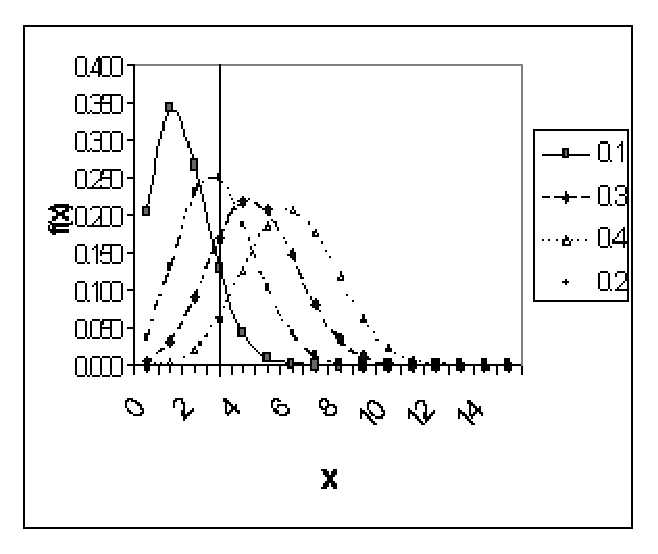
\includegraphics{./imatges/CriticalRegs.eps}
\end{center}
\caption{Regions cr\'{\i}tiques per al contrast sobre $p=0.1$}
\label{criticalregs}
\end{figure}

\subsubsection {Potencia del test $\mu=\mu_0$ vs $\mu> \mu_0$ o $\mu \neq \mu_0$}

Comencem en primer lloc per discutir la pot\`{e}ncia del test
\begin{eqnarray*}
H_0:\ \mu&=&\mu_0 \ (=8)\\
H_1:\ \mu &> & \mu_0\ (\mu=\mu_1>\mu_0).
\end{eqnarray*}
La pot\`{e}ncia del test \'{e}s la probabilitat de que una mostra es
trobi dins la regi\'{o} cr\'{\i}tica, si la hip\'{o}tesi nula \'{e}s
falsa, \'{e}s a dir:
\begin{eqnarray*}
\beta &=& P\left[ \bx \in W|H_0^c\right ]=\\
&=&P\left[ \bx |\ \overline{x}\geq \mu_0+z_{\alpha}\cdot
\sigma_0/\sqrt{n}|H_0^c\right ].
\end{eqnarray*}
Per calcular aquesta probabilitat no n'hi ha prou amb referir-se,
simplement, a "$H_0^c$". Cal especificar un valor de $\mu$, \'{e}s a
dir un valor concret sota la hip\'{o}tesi alternativa. Suposem que
si \'{e}s certa la hip\'{o}tesi alternativa aleshores $\mu=\mu_1>
\mu_0$. La pot\`{e}ncia del test ser\`{a}:
\begin{eqnarray}
\beta &=& P\left[ \bx |\ \overline{x}\geq \mu_0+z_{\alpha}\cdot
\sigma_0/\sqrt{n}|H_1\right ] \\
&=& P_{\mu=\mu_1} \left[\overline{x}\geq \mu_0+z_{\alpha}\cdot \sigma_0/\sqrt{n}\right ]\\
&=& P \left[\frac{\overline{x}-\mu_1}{\sigma_0/\sqrt{n}}\geq
\frac{\left(\mu_0+z_{\alpha}\cdot \sigma_0/\sqrt{n}\right)-\mu_1}{\sigma_0/\sqrt{n}}\right ]\\
&=& P \left[Z \geq
z_{\alpha}+\frac{\sqrt{n}}{\sigma_0}(\mu_0-\mu_1)\right ]
\label{PowerExp-1}
\end{eqnarray}
Si per exemple, segons la hip\'{o}tesi alternativa, $\mu_1$ val
respectivament $0.85$, $0.90$ o $0.95$ llavors la pot\`{e}ncia del
test val respectivament: $0.48$, $0.94$ i $0.999$ de manera que
l'error tipus II associat a cada hip\'{o}tesis alternativa ser\`{a}
$0.52$, $0.06$ i $0.001$ respectivament. Observi's que, com en
l'exemple anterior, quant m\'{e}s diferent sigui el valor de $\mu_1$
que proposa la hip\'{o}tesi alternativa del que diu la hip\'{o}tesi
nula m\'{e}s petit \'{e}s l'error de tipus II i m\'{e}s gran la
pot\`{e}ncia del test.

\subsection{Funci\'{o} de pot\`{e}ncia}
Els exemples anteriors posen de manifest que, donat un test de
nivell de significaci\'{o} $\alpha$ la seva capacitat per
discriminar entre dues hip\'{o}tesis dep\`{e}n de:
\begin{itemize}
\item La mida mostral
\item El valor concret del par\`{a}metre que proposa la hip\'{o}tesi
alternativa.
\end{itemize}
Podem generalitzar aquesta idea introduint la \em{funci\'{o} de
pot\`{e}ncia}.
\begin{definition}
Donat un model estad\'{\i}stic param\`{e}tric $\modest$ i un
contrast d'hip\'{o}tesis sobre $\theta$:
\begin{eqnarray*}
H_0:\ \theta &\in &\Theta_0 \ (\text{Sovint }\theta=\theta_0)\\
H_1:\ \theta &\in &\Theta_1=\Theta-\Theta_0,
\end{eqnarray*}
amb regi\'{o} cr\'{\i}tica de nivell de significaci\'{o} $\alpha$, $W_\alpha$
s'anomena funci\'{o} de pot\`{e}ncia del test a la funci\'{o} que, a cada
valor $\theta^*$ del par\`{a}metre li assigna la probabilitat de la
regi\'{o} cr\'{\i}tica suposant que $\theta=\theta*$, \'{e}s a dir:
\begin{eqnarray*}
\beta: &&\Theta \longrightarrow [0,1]\\
       &&\theta^* \longrightarrow
        \beta(\theta^*)=P_{\theta=\theta^*}(\bx\in W_\alpha)
\end{eqnarray*}
\end{definition}
La funci\'{o} de pot\`{e}ncia inclou dos dels conceptes que hem estudiat
en relaci\'{o} als errors de tipus I i II, i conv\'{e} no confondre-la
amb la \em{pot\`{e}ncia del test}:
\begin{itemize}
\item Si $\theta\in \Theta_0$ aleshores:
$$
\beta(\theta)=P_{\theta\in \Theta_0}(\bx\in W_\alpha) =P(\bx\in
W_\alpha|H_0)=\alpha=\text{ Probabilitat d'error tipus I}
$$
\item Si $\theta\in \Theta_1$ aleshores:
$$
\beta(\theta)=P_{\theta\in \Theta_1}(\bx\in W_\alpha) =P(\bx\in
W_\alpha|H_1)=\beta =\text{ Pot\`{e}ncia del test}.
$$
\end{itemize}

Fixat un valor de $\theta$ nom\'{e}s se sol poder augmentar la
pot\`{e}ncia augmentant la mida mostral $n$ tal i com mostra
l'expressi\'{o} \ref{PowerExp-1}. La figura \ref{PowerFunct} mostra la
funci\'{o} de pot\`{e}ncia per al test del segon exemple i diferents
valors '$n$. Com s'hi pot observar a un valor donat de $\theta$
li correspondran diferents valors de $\beta(\theta)$ tan m\'{e}s
grans com major sigui $n$.

\begin{figure}[ht]
\begin{center}
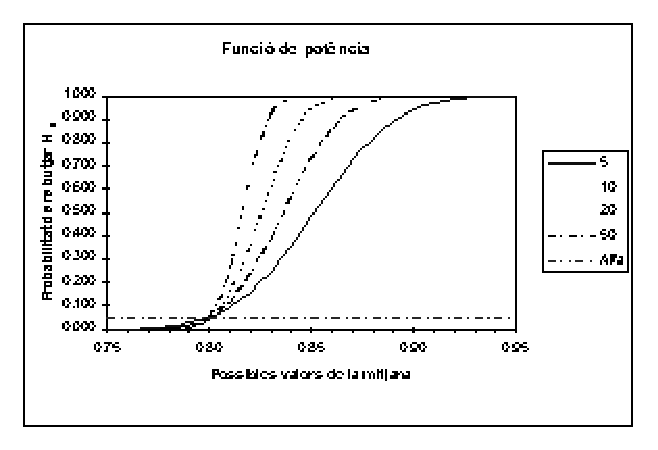
\includegraphics{./imatges/PowerFunct.eps}
\end{center}
\caption{Funci\'{o} de pot\`{e}ncia per al test $\mu=0.8$ vs $\mu>0.8$}
\label{PowerFunct}
\end{figure}

Observem l'expressi\'{o} \ref{PowerExp-1}
$$
\beta= P \left[Z \geq
\underbrace{z_{\alpha}+\frac{\sqrt{n}}{\sigma_0}(\mu_0-\mu_1)}_{z_\beta}\right]
$$
Podem fer-la servir per resoldre dos problemes d'inter\`{e}s for\c{c}a
pr\`{a}ctic. Suposant fixats $\alpha$, $\mu_0$ i $\mu_1$:
\begin{itemize}
\item Fixada una mida mostral determinar quina pot\`{e}ncia ($\rightarrow$ quin error de
tipus II) assolir\`{a} el test amb una mostra de mida $n$.
\item Fixada una pot\`{e}ncia $\beta$ podem determinar quina mida
mostral cal per assolir aquella pot\`{e}ncia, a\"{\i}llant el valor de $n$
\ref{PowerExp-1}:
$$
n=\left(\frac{z_\beta-z_\alpha}{\mu_0-\mu_1}\right)^2.
$$
\end{itemize}
Si en el segon exemple agafem $\alpha=0.05$, $\mu_0=0.8$,
$\mu_1=0.85$ podem respondre les dues q\"{u}estions b\`{a}siques:
\begin{itemize}
\item Quina ser\`{a} la probabilitat d'error tipus II si agafem una
mostra de mida $n=10$?
$$
\beta= P \left[Z \geq
z_{0.05}+\frac{\sqrt{10}}{0.07}(0.8-0.85)\right]=0.730\Rightarrow
$$
La probabilitat d'error tipus II \'{e}s 0.27
\item Quina mida mostral cal si volem que, com a molt, la
probabilitat d'error tipus II sigui 0.10 ($\Rightarrow
\beta=0.9$)?
$$
n=\left(\frac{z_{0.90}-z_{0.05}}{0.8-0.85}\right)^2=16.7\doteq 17
$$
\end{itemize}

\section{Tests de m\`{a}xima pot\`{e}ncia. Lema de Neymann-Pearson}

Com hem vist en les seccions anteriors, el plantejament que hem fet
de les proves d'hip\'{o}tesis t\'{e} l'inconvenient que nom\'{e}s
podem fixar una sola (probabilitat de ) tipus d'error cada vegada. A
la pr\`{a}ctica aix\'{o} es concreta en organitzar la prova de forma
que l'error que tingui ``pitjors'' conseq\"{u}\`{e}ncies sigui el de
tipus I, per al qual s'estableix una probabilitat petita $\alpha$.

Un cop fet aix\'{o} es procurar\`{a} escollir un test d'entre els de
nivell $\alpha$ que tingui la pot\`{e}ncia m\'{e}s alta possible,
\'{e}s a dir amb la m\'{\i}nima probabilitat d'error de tipus II.
Aquest problema no t\'{e} una soluci\'{o} general. El teorema
conegut com ``Lema de Neymann-Pearson" estableix una condici\'{o}
per a l'exist\`{e}ncia d'un test de m\`{a}xima pot\`{e}ncia quan
ambdues hip\'{o}tesis s\'{o}n simples. Sota certes condicions
m\'{e}s o menys restrictives el resultat es pot generalitzar al cas
en que la hip\'{o}tesis alternativa \'{e}s unilateral o,
excepcionalment per la fam\'{\i}lia exponencial, a hip\'{o}tesis
bilaterals.

\begin{definition}
Sigui ${\cal{D}}_\alpha$ el conjunt dels tests de nivell de
significaci\'{o} $\alpha$ per a un contrast d'hip\'{o}tesis simples.
Donats dos tests $\tau_1, \tau_2\in {\cal{D}}_\alpha$ direm que
$\tau_1$ \'{e}s m\'{e}s potent que $\tau_2$ si es compleix que:
$$
\beta_{\tau_1}>\beta_{\tau_2},
%\quad \forall \theta \in \Theta_1,
$$
\'{e}s a dir si \'{e}s compleix que la probabilitat d'error de tipus II,
$1-\beta$ \'{e}s m\'{e}s petita per $\tau_1$ que per $\tau_2$.
\end{definition}

\begin{definition}
Un test $\tau$ de la classe ${\cal{D}}_\alpha$  s'anomena de
m\`{a}xima pot\`{e}ncia si \'{e}s m\'{e}s potent que qualsevol altre test en
${\cal{D}}_\alpha$, \'{e}s a dir si
$$
\beta_{\tau}\geq \beta_{\tau'},\quad \forall \tau'\in
{\cal{D}}_\alpha.
$$ La regi\'{o} cr\'{\i}tica d'un test de m\`{a}xima pot\`{e}ncia s'anomena regi\'{o} cr\'{\i}tica \'{o}ptima.
\end{definition}

L'obtenci\'{o} de tests \'{o}ptims consistir\`{a} b\`{a}sicament en
fixar $\alpha$, habitualment en un valor petit, i mirar de
determinar $\tau$ de forma que sigui de m\`{a}xima pot\`{e}ncia. Una
eina per fer aix\'{o} ens la subministra el lema de Neymann-Pearson
que es presenta a continuaci\'{o}.

\subsection{Lema de Neymann-Pearson}

\begin{theorem}
Sigui $\bx$ una mostra aleat\'{o}ria simple d'una poblaci\'{o}
$\modest$ amb funci\'{o} de densitat $f(\bx;\theta)$ i funci\'{o} de
versemblan\c{c}a $L(\theta;\bx)$. Sigui el contrast d'hip\'{o}tesis
simples:
\begin{eqnarray*}
H_0:\quad \theta&=&\theta_0, \\
H_1:\quad \theta&=&\theta_1.
\end{eqnarray*}
 dues
Si existeix una constant positiva $K_\alpha$ tal que la regi\'{o}:
\begin{eqnarray*}
W_\alpha = \left\{ \bx:\
\frac{L(\theta_1;\bx)}{L(\theta_0;\bx)}\geq K_\alpha \right\}
\end{eqnarray*}
compleix que $P\{\bx \in W_\alpha\|H_0\}\leq \alpha$ aleshores
$W_\alpha$ \'{e}s la regi\'{o} cr\'{\i}tica \'{o}ptima de nivell
$\alpha$ per a aquest test.
\end{theorem}

No donarem la demostraci\'{o} d'aquest teorema que podeu veure a
la majoria dels textos de la bibliografia, com el de Fortiana i
Nualart  \cite{Fortiana-99} o Ruiz-Maya i Pliego
\cite{Ruiz-Maya-95}.

El resultat que presenta el teorema \'{e}s relativament
intu\"{\i}tiu. Si \'{e}s certa la hip\'{o}tesi alternativa la
versemblan\c{c}a ser\`{a} m\'{e}s gran amb $\theta_1$ que amb
$\theta_0$, de forma que \'{e}s d'esperar que, a partir d'un cert
valor, l'evid\`{e}ncia experimental continguda en la mostra sigui
m\'{e}s ``compatible'' amb la hip\'{o}tesi alternativa que la nula.
Aquest valor es determina a trav\'{e}s de la condici\'{o} de
regi\'{o} cr\'{\i}tica, \'{e}s a dir agafant-lo de forma que la
probabilitat de superar-lo si \'{e}s certa $H_0$ sigui un valor
petit, $\alpha$.

Per obtenir tests de m\`{a}xima pot\`{e}ncia mitjan\c{c}ant el lema
de Neymann-Pearson es comen\c{c}a per suposar que es disposa de la
regi\'{o} cr\'{\i}tica \'{o}ptima i es procura deduir del lema la
condici\'{o} que han de verificar els elements de la regi\'{o}
cr\'{\i}tica. Aquesta sol quedar en funci\'{o} d'una constant el
valor de la qual es calcula a partir de la condici\'{o} de regi\'{o}
cr\'{\i}tica. Veiem alguns exemples

\begin{example} \textbf{Test per a la mitjana d'una poblaci\'{o} normal}
\label{example-2-2}

Sigui $X\sim N(\mu,\sigma)$, amb $\sigma$ coneguda i el test
\beqa
H_0:\ \mu&=&\mu_0 \\
H_1:\ \mu &= & \mu_1. \eeqa Hem vist en l'exemple
[\ref{example-2-1}] que un test intu\"{\i}tiu per a aquest
problema consisteix en rebutjar $H_0$ si la mitjana de la mostra
supera un cert valor cr\'{\i}tic, massa gran per ser compatible
amb el valor $\mu_0$. El lema de Neymann-Pearson d\'{o}na lloc al
mateix test. Sigui: \beqa
L(\mu;\bx)=(2\pi\sigma^2)^{-n/2}\exp\left \{-\frac
1{2\sigma^2}\sum_{i=1}^n(x_i-\mu)^2\right\}, \eeqa d'on \beqa
\frac{L(\mu_1;\bx)}{L(\mu_0;\bx)}&=& \exp \left \{-\frac
1{2\sigma^2}
\sum_{i=1}^n[(x_i-\mu_1)^2-(x_i-\mu_0)^2]\right\},\\
&=& \exp \left \{-\frac 1{2\sigma^2}
\sum_{i=1}^n[2x_i(\mu_0-\mu_1)+(\mu_1^2-\mu_0^2)]\right\}. \eeqa La
regi\'{o} cr\'{\i}tica \'{o}ptima t\'{e} la forma
$$\frac{L(\mu_1;\bx)}{L(\mu_0;\bx)}\geq K_\alpha,\quad \text{o, equivalentment }\quad
ln\left [\frac{L(\mu_1;\bx)}{L(\mu_0;\bx)}\right]\geq
\ln(K_\alpha),$$ per alguna constant $K_\alpha$, \'{e}s a dir:
$$
-\sum_{i=1}^n[2x_i(\mu_0-\mu_1)+(\mu_1^2-\mu_0^2)]\geq 2\sigma^2
\ln(K_\alpha)
$$
o, expressada en funci\'{o} de la mitjana mostral:
$$
\overline{x}\geq\frac{\sigma^2
\ln(K_\alpha)}{n(\mu_1-\mu_0)}+\frac 12(\mu_0-\mu_1)=C_\alpha,
$$
on $C_\alpha$ \'{e}s una constant. Per determinar el valor de
$C_\alpha$ ignorem l'expressi\'{o} anterior i ens basem en el fet que
$W_\alpha$ \'{e}s regi\'{o} cr\'{\i}tica i per tant verifica que
$$
P\left\{\bx\in W_\alpha|H_0\right\}\leq \alpha.
$$
Si $H_0$ \'{e}s certa es t\'{e} que $\overline{X}\sim
N(\mu_0,\sigma^2/n)$, de forma que l'expressi\'{o} anterior esdev\'{e}:
$$
P\left\{\bx\in W_\alpha|H_0\right\}= P\left\{\overline {X}\geq
C_\alpha\right\}=\alpha,
$$
d'on, com ja hav\'{\i}em vist en l'exemple se'n surt que
$$
C_\alpha= \mu_0+z_{\alpha}\cdot \sigma/\sqrt{n}.
$$

Observem que si $\mu_1$ hagu\'{e}s estat $< \mu_0$ llavors el signe de
la desigualtat hauria canviat al dividir per $(\mu_1-\mu_0)$ amb
la qual cosa la regi\'{o} cr\'{\i}tica hauria estat de la forma
$\overline{X}<{C'}_{\alpha}$ tal i com suggereix la intu\"{\i}ci\'{o} en
aquest cas.

\end{example}

\section{Tests d'hip\'{o}tesis compostes}

En molts problemes de contrastos les hip\'{o}tesis no s\'{o}n
necess\`{a}riament simples, especialment la hip\'{o}tesi
alternativa. Si per exemple estem estudiant si uns cigarrets baixos
en nicotina contenen ``com a molt'' $0.8$ mg de nicotina les
hip\'{o}tesis raonables no serien: \beqa
H_0:\ \mu&=& \mu_0 \\
H_1:\ \mu &=& \mu_1,\eeqa
sino
\beqa
H_0:\ \mu&\leq&\mu_0 \\
H_1:\ \mu &> & \mu_1.
\eeqa

En l'exemple [\ref{example-2-2}], per al contrast simple $\mu=
\mu_0$ enfront $\mu= \mu_1$ hem obtingut una regi\'{o} cr\'{\i}tica
que no depen del valor de $\mu_1$ sin\'{o} \'{u}nicament de si
\'{e}s major o menor que $\mu_0$. Aix\'{o} vol dir que la regi\'{o}
cr\'{\i}tica ser\`{a} la mateixa per qualsevol valor de $\mu_1 >
\mu_0$ o, respectivament $\mu_1<\mu_0)$. Aquest resultat es pot
generalitzar de la manera seg\"{u}ent.
\begin{proposition}
Sigui $W_\alpha$ la regi\'{o} cr\'{\i}tica \'{o}ptima  per a un test
d'hip\'{o}tesis simples $H_0:\ \theta= \theta_0$ enfront $H_1:
\theta = \theta_1$. Si $W_\alpha$ no dep�n del valor de $\theta_1$
per a qualsevol $\theta_1< \theta_0$ (respectivament $\theta_1>
\theta_0$) aleshores $W_\alpha$ \'{e}s la regi\'{o} cr\'{\i}tica
\'{o}ptima per al test d'hip\'{o}tesis simple enfront composta
$H_0:\ \theta= \theta_0$ enfront $H_1: \theta < \theta_1$
(respectivament  $\theta_1> \theta_0$) .
\end{proposition}
\begin{proof}
$W_\alpha$ \'{e}s la regi\'{o} cr\'{\i}tica \'{o}ptima per al test
$H_0:\ \theta= \theta_0$ enfront $H_1: \theta = \theta_1$. Suposem
que $W_\alpha$ no \'{e}s RCO per al test $H_0:\ \theta= \theta_0$
enfront $H_1: \theta < \theta_1$. Aix\'{o} vol dir que existir\`{a}
alguna altra regi\'{o} cr\'{\i}tica $W_\alpha'$ tal que,
\begin{equation}
\text{donat }\theta_1' < \theta_0\longrightarrow P_{\theta_1'}
(W_\alpha')>P_{\theta_1'}(W_\alpha).\label{absurd}
\end{equation}
Per\'{o} aix\'{o} no \'{e}s possible ja que, si $W_\alpha$ no dep�n
del valor de $\theta_1$ tamb\'{e} ha de ser RCO per al test $H_0:\
\theta= \theta_0$ enfront $H_1: \theta = \theta_1'$, \'{e}s a dir
cal que $P_{\theta_1'}(W_\alpha')>P_{\theta_1'}(W_\alpha)$ que
contradiu \ref{absurd}. La contradicci\'{o} prov\'{e} de suposar que
$W_\alpha$ no \'{e}s RCO i per tant queda establert que ha de
ser-ho.
\end{proof}

\begin{definition}Si �s possible trobar una regi� cr�tica $W^*$ la pot�ncia de
la qual sigui m�xima sigui quin sigui el valor de $\theta$
determinat en la hip�tesis alternativa, diem que $W^*$ �s una regi�
cr�tica �ptima uniformement. El test associat a una regi� cr�tica
�ptima uniformement s'anomena test uniformement m�s potent o U.M.P.
\end{definition}

En general, per�, per als contrastos unilaterals i bilaterals no
es pot assegurar que existeixi  un test U.M.P. Hi ha dues formes
d'abordar aquest problema que ens duen a solucions parcials per a
alguns casos: Es pot for�ar el model probabil�stic, requerint
alguna propietat addicional de la fam�lia de probabilitats o es
pot restringir la classe de tests entre els quals es busca el
test �ptim.

La primera aproximaci� ens duu a considerar nom�s aquelles
fam�lies de probabilitats en les quals la ra� de versemblances
que apareix en el lema de Neymann-Pearson es pot expressar com
una funci� mon�tona d'un estad�stic. Intu�tivament en aquest cas
ser� possible ``a�llar la condici� de regi� cr�tica" en funci�
d'aquest estad�stic. Les fam�lies que tenen aquesta propietat
s'anomenen fam�lies amb {\em ra� de versemblan�a mon�tona}.

Una segona aproximaci� s'obt� en observar que, si no es busca el
test U.M.P. entre tots els tests possibles sin� �nicament entre
aquells que verifiquen una determinada restricci�, molt raonable,
aleshores �s possible trobar tests U.M.P. per alguns contrastos
d'hip�tesis alternatives bilaterals. La restricci� consisteix en
cercar nom�s entre els tests amb probabilitat d'error de tipus II
menor que $1-\alpha$. Per� aix� �s molt raonable ja que, el que vol
dir �s que no es tindran en compte aquells tests on sigui m�s
probable acceptar $H_0$ equivocadament (error de tipus II) que amb
ra� (decisi� correcta amb probabilitat $1-\alpha$).

\subsection{Fam�lies amb ra� de versemblances mon�tona}

En l'exemple anterior hem vist que, si en el test d'hip\'{o}tesis
simples $H_0:\ \theta= \theta_0$ enfront $H_1: \theta = \theta_1$
s'obt�, aplicant el lema de Neyman-Pearson, que la regi� cr�tica,
$W_\alpha$, no dep�n del valor de $\theta_1$ aleshores $W_\alpha$
\'{e}s la regi\'{o} cr\'{\i}tica \'{o}ptima per al test
d'hip\'{o}tesis simple enfront composta $H_0:\ \theta= \theta_0$
enfront $H_1: \theta < \theta_1$.

Una pregunta raonable �s si ser� sempre possible procedir
d'aquesta forma o, en tot cas, quan �s possible trobar una regi�
cr�tica �ptima que no depengui de $\theta_1$ sin� nom�s de si
$\theta_0> \theta_1$ o al contrari. La caracteritzaci� de les
fam�lies de probabilitats per a les quals aix� �s possible es fa
fent servir el concepte de {\em ra� de versemblan�a mon�tona}.

\begin{definition}
Sigui $\modest$ un model estad�stic, $f_\theta$ la fam�lia de
probabilitats associada al model i $\bx$ una mostra aleat�ria
simple d'$X$. Diem que la fam�lia de probabilitats $f_\theta,\
\theta\in\Theta$ t� ra� de versemblan�a mon�tona en l'estad�stic
$T(\bx)$ si, $\forall \theta_1>\theta_0$ i, sempre que
$f_{\theta_1}(\bx)\neq f_{\theta_0}(\bx)$ es t� que
$$
R(\bx)=\frac{f_{\theta_1}(\bx)}{f_{\theta_0}(\bx)},
$$
�s una funci� no decreixent de $T(\bx)$.
\end{definition}

\begin{example}
En una fam�lia amb llei de Poisson suposem $\lambda_1>\lambda_2$ i
una m.a.s. $\bx$. La funci� de versemblan�a de la mostra �s:
$$
L(\lambda;\bx)=\exp{-n\,\lambda}\frac{\lambda^{\sum x_i}}{x_i!}.
$$
Aleshores:
\beqa
R(\bx)&=& \frac{\exp{-n\,\lambda_1}\frac{\lambda_1^{\sum
x_i}}{x_i!}}
{\exp{-n\,\lambda_2}\frac{\lambda_2^{\sum x_i}}{x_i!}}\\
&=&\exp{-n(\lambda_1-\lambda_2)}\left(\frac{\lambda_1}{\lambda_2}\right)^
{\sum x_i}.
\eeqa
Prenent logaritmes tindrem
\beqa
\log R(\bx)&=&
\underbrace{-n(\lambda_1-\lambda_2)}_A+\underbrace{\sum
x_i}_T(\bx)\cdot \underbrace{\log
\left(\frac{\lambda_1}{\lambda_2}\right)}_B\\
&=&A+B\cdot T(\bx),\quad, B>0,
\eeqa
i per tant la fam�lia de Poisson t� ra� de versemblan�a en
$T(\bx)=\Sumin x_i$.
\end{example}

\begin{example}
La fam�lia exponencial uniparam�trica t� ra� de versemblances
mon�tona. Efectivament donada
$$
L(\theta;\bx)=C(\theta)h(\bx)\exp{Q(\theta)T(\bx)},
$$
suposem $\theta_1>\theta_2$.
\beqa
R(\bx)&=&\frac{C(\theta_1)h(\bx)\exp{Q(\theta_1)T(\bx)}}
{C(\theta_2)h(\bx)\exp{Q(\theta_2)T(\bx)}}\Longrightarrow\\
\log R(\bx)&=&\left[\log\frac{C(\theta_1)}{C(\theta_2)}\right]+
\left(Q(\theta_1)-Q(\theta_2)\right)T(\bx).
\eeqa
Si $Q(\theta)$ �s creixent (decreixent) aleshores $R(\bx)$ t� RVM
en $T(\bx)$ (en $-T(\bx)$). Si no ho �s �s possible fer-la
esdevenir mitjan�ant una reparametritzaci�.
\end{example}

\begin{example}
Sigui $X\sim {\cal C}(1,\theta)$ una distribuci� de Cauchy.
LLavors, donats $\theta_1> \theta_2$ es t�:
$$
R(\bx)=\frac{1+(x-\theta_1)^2}{1+(x-\theta_2)^2}\longrightarrow
1,\quad \text{quan } x\rightarrow \pm \infty,
$$
de manera que ${\cal C}(1,\theta)$ no t� RVM.
\end{example}

L'inter�s del concepte de RVM resideix en el teorema que es presenta
a continuaci�, que estableix l'exist�ncia de tests UMP d'hip�tesis
unilaterals per a les fam�lies amb ra� de versemblan�a mon�tona.

\begin{theorem}\textbf{Karlin-Rubin}
Sigui $f(x;\theta), \{\theta\in\Theta\}$ una fam�lia de
probabilitats amb ra� de versemblan�a mon�tona en l'estad�stic
$T(\bX)$. Per contrastar la hip�tesis $H_0:\ \theta=\theta_0
(\theta\leq \theta_0),\ \theta_0\in \Theta_0$ enfront $H_1:\ \theta>
\theta_0$ qualsevol test de mida $\alpha$ amb regi� cr�tica
\begin{equation}
W_\alpha=\left\{\bx|T(\bx)\geq
c_\alpha\right\}\label{test-K-R}
\end{equation} t� funci� de pot�ncia no decreixent i �s U.M.P. entre els
tests de mida $\alpha$ per a aquesta hip�tesis.

A m�s a m�s $\forall\alpha\in[0,1]$ i $\forall\theta\in\Theta$
existeix $c_\alpha$ tal que  tal que el test descrit a
\ref{test-K-R} sigui U.M.P. de mida $\alpha$ per contrastar $H_0$
enfront $H_1$.

\end{theorem}
Podeu veure la demostraci� d'aquest teorema, en versi�
aleatoritzada, a Rohatgi(\cite{Rohatgi-75}).

\begin{example}
En una distribuci� uniforme $X\sim[0,\theta]$ volem contrastar la
hip�tesis : \beqa H_0:&&\ \theta=\theta_0 \\ H_1:&&\
\theta>\theta_0.\eeqa Comencem per determinar si es tracta d'una
fam�lia amb RVM. Donada una mostra aleat�ria simple, $\bx$ la
versemblan�a del model �s:
$$
L(\theta;\bx)=\frac 1{\theta^n}\textbf{1}_{[0\leq \max x_i\leq
\theta ]}(\bx).
$$
Suposem $\theta_1>\theta_2$ i considerem la ra�:
\beqa
\frac{f_{\theta_1}(\bx)}{f_{\theta_2}(\bx)}&=& \frac{\frac
1{\theta_1^n}\textbf{1}_{[0\leq \max x_i\leq \theta_1
]}(\bx)}{\frac 1{\theta_2^n}\textbf{1}_{[0\leq \max x_i\leq
\theta_2]}(\bx)}\\
&=&\left(\frac{\theta_2}{\theta_1}\right)^n
\frac{\textbf{1}_{[0\leq \max x_i\leq \theta_1]}(\bx)}
{\textbf{1}_{[0\leq \max x_i\leq \theta_2]}(\bx)}.
\eeqa
Sigui
$$
R(\bx)=\left\{
\begin{array}{ll}
  1 & \max x_i \in [0,\theta_2] \\
  \infty & \max x_i \in [\theta_2,\theta_1 ]
\end{array}
\right.
$$
Si definim $R(\bx)=\infty$ si $ \max x_i> \theta_1$ aleshores
$\frac{f_{\theta_1}(\bx)}{f_{\theta_2}(\bx)}$ �s una funci� no
decreixent de l'estad�stic $$T(\bX)=\max_{1\leq i\leq n} X_i$$ i
la fam�lia de densitats uniformes t� ra� de versemblan�a mon�tona
en $T(\bX)$. En conseq��ncia, pel teorema de Karlin-Rubin el test
\begin{equation}
W_\alpha=\left\{\bx|T(\bx)\geq c_\alpha\right\},
\end{equation}
�s un test UMP per a les hip�tesis \beqa H_0:&&\ \theta \leq
\theta_0
\\ H_1:&&\ \theta>\theta_0.\eeqa
El punt cr�tic $c_\alpha$ es determina per la condici� de que
$W_\alpha$ sigui regi� cr�tica, �s a dir:
\beqa
P\left\{\bx|T(\bx)\leq c_\alpha|H_0\right\}&=&\\
 \left( \frac{c_\alpha}{\theta_0}\right)^n &=&1-\alpha,
\eeqa
d'on rebutjarem $H_0$ si ${\displaystyle\max_{1 \leq i\leq n} x_i
\geq \theta_0 (1-\alpha)^{\frac 1n}}$.
\end{example}

\subsection{Tests sense biaix o centrats}
Una segona alternativa, a l'hora de buscar tests U.M.P. per
contrastos d'hip�tesis compostes �s restringir-nos als tests
centrats o sense biaix.
\begin{definition}
Un test de mida $\alpha$ i regi� cr�tica $W_\alpha$ per a les
hip�tesis $H_0:\ \theta\in \Theta_0$ enfront $H_1:\ \theta\in
\Theta_1$ s'anomena centrat o sense biaix si es verifica que la
pot�ncia del test �s m�s gran o igual que el nivell de significaci�
per a qualsevol valor de la hip�tesis alternativa �s a dir si:
$$
\beta(\theta)=P\left\{\bx \in W_\alpha|H_1\right\}\geq \alpha,\
\forall \theta \in \Theta_1.
$$
\end{definition}
Com ja hem comentat aquest requeriment �s molt natural ja que
nom�s vol dir que la probabilitat de rebutjar $H_0$
(correctament) quan �s falsa ha de ser m�s gran que la
probabilitat de fer-ho (incorrectament) quan �s certa.

Si ens restringim als tests sense biaix �s possible establir
l'exist�ncia de tests U.M.P., que en aquest cas s'anomenen
U.M.P.S.B. per a la fam�lia exponencial uniparam�trica. Els
teoremes seg�ents estableixen aquesta propietat i donen alguns
d'aquests tests pel cas de la distribuci� normal. Les
demostracions es poden trobar a Lehman (\cite{Lehman-86}).

\begin{theorem}
Si la fam�lia $\left\{ f (x;\theta),\ \theta\in \Theta \right \}$
�s exponencial uniparam�trica aleshores existeix un test U.M.P.
sense biaix de mida $\alpha$ per al contrast bilateral  $H_0:\
\theta=\theta_0$ enfront $H_1:\ \theta\neq \theta_0$.
\end{theorem}

\begin{theorem}
Sigui $\Sample$ una mostra aleat�ria simple d'una variable amb
distribuci� $N(\mu,\sigma)$.
\begin{enumerate}
\item Si $\sigma^2$ �s coneguda aleshores per contrastar
$H_0:\ \mu=\mu_0$ enfront $H_1:\ \mu\neq\mu_0$ el test consistent
en rebutjar $H_0$ si $|Z|>\zem$, on
$$Z=\frac{\ds{\bar{X}-\mu_0}}{\ds\sqrt{\sigma^2/n}} \sim N(0,1)$$
�s U.M.P. sense biaix de nivell $\alpha$.
\item Si $\sigma^2$ �s desconeguda aleshores per contrastar $H_0:\ \mu=\mu_0$
enfront $H_1:\ \mu\neq\mu_0$ el test consistent en rebutjar $H_0$
si $|T|> t(\alpha,n-1)$, on
$$T=\frac{\ds{\bar{X}-\mu_0}}{\ds{S}}\sqrt{n-1} \sim t(n-1)$$ �s
U.M.P. sense biaix de nivell $\alpha$.
\item Per contrastar $H_0:\ \sigma^2=\sigma_0^2$ enfront $H_1:\ \sigma^2=\sigma_0^2$
el test consistent en rebutjar $H_0$ si
$$\chi^2 >\chi_{(n-1),\alpha/2}  \text{ o } \chi^2<\chi_{(n-1),1-\alpha/2},$$ on
$$\chi^2=\frac{\ds{(n-1)\hat{S}^2}}{\ds{\sigma_0^2}} \sim
\chi^2(n-1),$$ �s U.M.P. sense biaix de nivell $\alpha$.
\end{enumerate}
\end{theorem}
Els valors $\zem$, $t(\alpha,n-1)$ i $\chi_{(n-1),\alpha/2}$ s�n
respectivament els percentils $1-\alpha$ de les distribucions
$N(0,1)$ $t$ de Student amb $n-1$ graus de llibertat i $\chi^2$
amb $n-1$ graus de llibertat.

\begin{theorem}
Sigui $\bX_1$, una mostra d'una poblaci� normal
$N(\mu_1,\sigma_1)$ i $\bX_2$ una altra mostra provinent d'una
poblaci� $N(\mu_2, \sigma_2)$ independent de l'anterior.
\begin{enumerate}
\item Si $\sigma_1^2,\sigma_2^2$ s�n conegudes, aleshores per
contrastar $H_0: \mu_1-\mu_2$ enfront d'$H_1: \mu_1 \neq \mu_2$,
el test consistent en rebutjar $H_0$ si $|Z| >\zem$ on
$$
Z=\frac{\ds{(\bar{X}_1-\bar{X}_2)-d_0}}
{\ds{\sqrt{\frac{\sigma_1\sp 2}{n_1}+\frac{\sigma_2\sp 2}{n_2}}}}
\sim N(0,1),
$$
�s U.M.P. sense biaix de nivell $\alpha$.
\item Si $\sigma_1^2, \sigma_2^2$ s�n desconegudes per� iguals,
$\sigma_1^2=\sigma_2^2$ aleshores per contrastar $H_0:
\mu_1-\mu_2$ enfront d'$H_1: \mu_1 \neq \mu_2$, el test
consistent en rebutjar $H_0$ si $|T| > t(\alpha,n_1+n_2-2)$ on
$$
T=\frac{\ds{(\bar{X}_1-\bar{X}_2)-d_0}}%
{\sqrt{\frac{\ds{(n_1S_1\sp 2 + n_2 S_2\sp 2)\,(n_1+n_2)}}
{\ds{(n_1+n_2-2)(n_1\,n_2)}}}} \sim t(n_1+n_2-2)
$$
�s U.M.P. sense biaix de nivell $\alpha$.
\item Per contrastar $H_0: \sigma_1\sp 2=\sigma_2\sp 2$ enfront
d'$H_1: \sigma_1\sp 2 \neq \sigma_2\sp 2$ el test consistent en
$$
\text {rebutjar $H_0$ si } F > F_{n_2,\alpha/2}^{n_1} \mbox{ o }
F< F_{n_2,1-\alpha/2}^{n_1},
$$
on
$$
F=\frac{\ds{\hat{S}_1\sp 2}}{\ds{\hat{S}_2\sp 2}} \sim
F(n_1-1,n_2-1)
$$
�s U.M.P. sense biaix de nivell $\alpha$.
\end{enumerate}
\end{theorem}
Els valors $\zem$, $t(n_1+n_2-2)$ i $ F_{n_2,\alpha/2}^{n_1}$ s�n
respectivament els percentils $1-\alpha$ de les distribucions
$N(0,1)$, $t$ de Student amb $n-1+n_2-2$ graus de llibertat i $F$
de Fisher amb $n_1, n_2$ graus de llibertat.

\subsection{Exemples}
Podeu trobar exemples resolts de tots aquests tests al cap�tol 6
("An�lisis estad�stico Normal") de Cuadras (\cite{Cuadras-00}).

\chapter{M\`{E}TODES DE CONSTRUCCI\'{O} DE TESTS}

En el cap\'{\i}tol anterior hem presentat els conceptes b\`{a}sics de
proves d'hip\`{o}tesis i hem vist que, donada la naturalesa
antag\`{o}nica dels errors de tipus I i tipus II, l'ideal \'{e}s disposar
de tests uniformement de m\`{a}xima pot\`{e}ncia. Tamb\'{e} hem vist que aix\`{o}
nom\'{e}s \'{e}s possible en determinats casos, com quan ambdues
hip\`{o}tesis s\'{o}n simples o sota certes restriccions sobre la fam\'{\i}lia
de probabilitats (fam\'{\i}lies amb ra\'{o} de versemblan\c{c}a mon\`{o}tona) o
sobre els tests (tests centrats en la fam\'{\i}lia exponencial
uniparam\`{e}trica).

En la pr\`{a}ctica desitgem disposar de m\`{e}todes generals per
construir contrastos basats en principis raonables que permetin
dissenyar tests adients en qualsevol circumst\`{a}ncia. En aquest
cap\'{\i}tol considerarem dos d'aquests m\`{e}todes: \bit
\item El test de la ra\'{o} de versemblances
\item Els tests basats en intervals de confian\c{c}a
\eit

\section{El test de la ra\'{o} de versemblances}
El {\em test de ra\'{o} de versemblances}\footnote{Aquesta part ha estat desenvolupada per la Dra. Marta Cubedo}, \'{e}s un m\`{e}tode general per
construir tests (regions cr\'{\i}tiques) per a un problema qualsevol
de contrast d'hip\`{o}tesis. T\'{e} l'inconvenient que no d\'{o}na lloc de
forma autom\`{a}tica a tests UMP, tot i que, si existeix el test UMP
per al problema en q\"{u}esti\'{o} llavors el test el proporciona. A
canvi d'aquest inconvenient t\'{e} l'avantatge de ser for\c{c}a intu\"{\i}tiu
i tenir bones propietats, asimpt\`{o}tiques, \'{e}s a dir funciona b\'{e}
especialment amb mostres grans.

Considerem un model estad\'{\i}stic $\modest$ i sigui
$\,x=(x_{1},x_{2}, \cdots ,x_{n})\,$ una mostra aleat\`{o}ria simple
d'una poblaci\'{o} amb densitat de probabilitat $\,f(x;\theta)\,$ on
$\,\theta = ({\theta}_{1},\,{\theta}_{2}, \cdots
,{\theta}_{k})\,$ es el vector de par\`{a}metres. Suposarem  endem\'{e}s
que la funci\'{o} de veresemblan\c{c}a
$$L(x;\theta )=f(x_{1};\theta ) \cdots f(x_{n};\theta )$$
\'{e}s estrictament positiva $\,L(x;\theta) >0 \hspace{0.5cm} \forall
x\in \Omega $

%Recordem brevemente la definici�n de {\bf estimador
%m\'{a}ximo-veros\'{\i}mil}:
%
%\vspace{15pt} Dada la funci�n de versemblan\c{c}a $\,L(x;\theta)\,$
%escogeremos la aproximaci�n del par\'{a}metro desconocido
%$\,\theta\,$ que haga m\'{a}ximo el valor de $\,L(x;\theta)$.
%
%\vspace{12pt}
%Para ello, suponiendo $\,L\,$ diferenciable respecto a $\,\theta\,$ y
%sin un m\'{a}ximo en la frontera del dominio, obtendremos la estimaci�n
%m\'{a}ximo-veros\'{\i}mil resolviendo el sistema de ecuaciones:
%
%\vspace{10pt}
%$$\left\{ \begin{array}{lll}
%{\displaystyle \frac{\partial L}{\partial {\theta}_{1}}} & = & 0 \\
%           \vdots                                   &   &    \\
%{\displaystyle \frac{\partial L}{\partial {\theta}_{k}}} & = & 0
%          \end{array} \right.  $$
%
%$$\left\{ \begin{array}{lll}
%{\displaystyle \frac{\partial \ln{L}}{\partial {\theta}_{1}}} & = & 0 \\
%           \vdots                                        &   &    \\
%{\displaystyle \frac{\partial \ln{L}}{\partial {\theta}_{k}}} & = & 0
%          \end{array} \right.  $$
% El valor resultante $\,\hat {\theta}\,$ ser\'{a} un m\'{a}ximo si la
%matriz Hessiana es definida ne\-ga\-ti\-va.
%
%\vspace{15pt} En la pr\'{a}ctica se obtiene as\'{\i} dado que el m\'{a}ximo
%del logaritmo de la funci�n de versemblan\c{c}a suele ser m\'{a}s
%manejable y, al ser el logaritmo una funci�n mon�tona, el
%resultado es el mismo que sin el logaritmo.
%
%\vspace{15pt}

Donada una partici\'{o} de l'espai de par\`{a}metres $\,\Theta =
{\Theta}_{0} \cup {\Theta}_{1}\,$ siguin:
$$L(x;{\Theta}_{0})=\sup_{\theta \in {\Theta}_{0}} {L(x;\theta)}
\hspace{1cm} L(x;\Theta)=\sup_{\theta \in \Theta} {L(x;\theta)}$$
\begin{definition}
Donat un model estad\'{\i}stic, $\modest$ i un problema de contrast
d'hip\`{o}tesis sobre $\Theta$, $H_0:\ \theta \in\Theta_0$, $H_1:\
\theta \in(\Theta-\Theta_0)=\Theta_1$, s'anomena ra\'{o} de
versemblances al quocient
$$\Lambda {(x)}=\frac{L(x;{\Theta}_{0})}{L(x;\Theta)}.$$
Observi's que $\,0 \leq \Lambda (x)\leq 1$.
\end{definition}

\subsection{Construcci\'{o} de tests de ra\'{o} de versemblances}

Sigui $\,H_{0}\,$ la hip\`{o}tesis que es vol provar. Com ja hem vist
$\, H_{0}\,$ imposa certes restriccions sobre els valors de
$\,\theta\,$ i determina un subconjunt de $\,\Theta\,$ que
representarem per $\,{\Theta}_{0}\,$.

Recordem que, donada una m.a.s. $\,x=(x_{1}, \cdots , x_{n})\,$ la
funci\'{o} de versemblan\c{c}a corresponent \'{e}s:
$$L(x;\theta)=f(x_{1};\theta) \cdots f(x_{n};\theta)$$
on suposem fixes els valors mostrals $\,x_{i}, \,\, i=1, \cdots
,n\,$ i fem variar $\,\theta\,$ sobre $\,\Theta\,$ podrem
calcular el suprem de la funci\'{o} de versemblan\c{c}a, que amb la
notaci\'{o} definida anteriorment
$$L(x;\Theta)=\sup_{\theta \in \Theta} {L(x;\theta)}.$$
Fent el mateix amb $\,{\Theta}_{0}\,$ i el suprem de la funci\'{o} de
versemblan\c{c}a restringit a $\,{\Theta}_{0}\,$ es representar\`{a} com:
$$L(x;{\Theta}_{0})=\sup_{\theta \in {\Theta}_{0}} {L(x;\theta)}.$$
En la pr\`{a}ctica els ``suprems'' de les expressions anteriors seran
els ``m\`{a}xims'' i s'obtindran a partir del c\`{a}lcul dels m\`{a}xims d'una
funci\'{o} real i, en el caso del subespai $\,\Theta_0 \,$, de m\`{a}xims
amb restriccions.

La idea que fa que aquest test sigui for\c{c}a intu\"{\i}tiu \'{e}s la
seg\"{u}ent: Si per a una mostra donada el valor de
$\,{\Lambda}(x)\,$ es gran (pr\`{o}xim a 1), tindrem que el valor de
$\,L(x;{\Theta}_{0})\,$ ser\`{a} pr\`{o}xim al valor de $\,L(x;\Theta)\,$.
Aix\`{o} voldr\`{a} dir que no podrem obtenir un valor massa m\'{e}s gran de
$\,L(x;\theta)\,$ al buscar $\,\theta\,$ en tot l'espai de
par\`{a}metres $\,\Theta\,$, del que es pugui obtenir buscant
$\,\theta\,$ en $\,{\Theta}_{0}\,$. Quan aix\`{o} sigui aix\'{\i} ser\`{a}
indicatiu de que la hip\`{o}tesi nul.la $\,H_{0}\,$ \'{e}s certa.

En vista de l'anterior podem donar la definici\'{o} seg\"{u}ent:
\begin{definition}
El test de ra\'{o} de versemblances que contrasta les hip\`{o}tesis:

\vspace{10pt} \hspace{0.5cm}$H_{0}:\,\theta \in {\Theta}_{0}$
\hspace{0.5cm} contra \hspace{0.5cm} $H_{1}:\,\theta \in
{\Theta}_{1}=\Theta \setminus {\Theta}_{0}$ \vspace{12pt} al
nivell de significaci\'{o} $\,\alpha \in (0,1)\,$ \'{e}s el que t\'{e} com
regi\'{o} cr\'{\i}tica:
$$W_{\alpha}=\{ x, \,\,\, \Lambda (x) < c_{\alpha} \},$$
on $\,c_{\alpha}\,$ es determina de manera que l'error de primera
esp\`{e}cie sigui menor o igual que $\,\alpha\,$, \'{e}s a dir:
$$P_{\theta} (W_{\alpha}) \leq \alpha, \hspace{0.5cm} \forall \theta \in
{\Theta}_{0}$$ (Probabilitat de rebutjar $H_{0}$ quan \'{e}s certa
$\leq \alpha$).
\end {definition}

\subsubsection{Observacions}

\begin{enumerate}
\item At\`{e}s que $\,0 \leq \Lambda (x) \leq 1\,$, tamb\'{e} es t\'{e} que
    $\,0 \leq c_{\alpha} \leq 1$.
\item Si el model estad\'{\i}stic \'{e}s tal que existeix l'estimador
del m\`{a}xim de versemblan\c{c}a  $\,\hat{\theta} (x)\,$ per a
$\,\theta\,$, llavors el denominador de $\,\Lambda (x)\,$ ser\`{a}
$\,L(x;\Theta)= L(x;\hat {\theta} (x))\,$ i en el numerador es
considerar\`{a} l'estimador del m\`{a}xim de versemblan\c{c}a restringit a
$\,{\Theta}_{0}$.
\item Si considerem $\,{\Theta}_{0}=\{ {\theta}_{0} \} \,$ i
$\,{\Theta}_{1}=\{ {\theta}_{1} \} \,$ aleshores el test de la
ra\'{o} de versemblances coincideix amb el que obtindr\'{\i}em aplicant el
m\`{e}tode de Neyman-Pearson (podeu veure'n la prova en l'appendix d'aquest cap\'{\i}tol).

\end{enumerate}


\begin{example}\textbf{Contrast per a la mitjana d'una poblaci\'{o} normal amb vari\`{a}ncia desconeguda}

Considerem una m.a.s. de mida $\,n,\,$ $\,x=(x_{1},
\cdots,x_{n})\,$  d'una variable aleat\`{o}ria $\,X\,$ que segueix
una dis\-tri\-bu\-ci\'{o} $\,N({\mu} , {\sigma}^2)\,$.

Es desitja contrastar la hip\`{o}tesi seg\"{u}ent:
$$H_{0}:\mu={\mu}_{0}\, \hspace{0.5cm} \text{contra} \hspace{0.5cm}
H_{1}:\mu \neq {\mu}_{0}.$$ Observem que \textbf{No es tracta
d'hip\`{o}tesis simples} ja que:
\begin{eqnarray*}
\Theta&=&\left \{ \theta=(\mu,{\sigma}^2) \in {{\bf R}\times {\bf
R}^{+}} \right \} \text{ i}\\
{\Theta}_{0}&=&\left \{ \theta=({\mu}_{0},{\sigma}^{2}),\,\,
{\sigma} \in {\bf R}^{+} \right \} \end{eqnarray*} Els estimadors
del m\`{a}xim de versemblan\c{c}a s\'{o}n respectivament la mitjana i la
vari\`{a}ncia mostrals. Tenim doncs que:
$$L(x;\Theta)=L(x;\hat{\theta} (x))=L(x;(\bar{x}_{n},S_{n}))={\left[
\frac{2\pi}{n} \sum_{i=1}^{n} {(x_{i}-\bar{x}_{n})^2}
\right]}^{-\frac{n}{2}}e^{-\frac{n}{2}}$$ on
$$\bar{x}_{n}=\frac{1}{n}\sum_{i=1}^{n} {x_{i}} \hspace{1cm}
S_{n}=\frac{1}{n}\sum_{i=1}^{n} {(x_{i}-\bar{x}_{n})^2}$$ y at\`{e}s
que
$$L(x;(\mu , {\sigma}^2))=(2\pi {\sigma}^2)^{-\frac{n}{2}}exp \left[
\frac{-1}{2{\sigma}^2}\sum_{i=1}^{n} {(x_{i}-\mu )^2} \right] $$
el valor de $\,{\sigma}^2\,$ que maximitza la funci\'{o} fixada
$\,\mu={\mu}_{0}\,$ \'{e}s:
$$\frac{1}{n} \sum_{i=1}^{n} {(x_{i}-{\mu}_{0})^2} $$
En conseq\"{u}\`{e}ncia:
$$L(x;{\Theta}_{0})=L \left( x;({\mu}_{0},\frac{1}{n}\sum_{i=1}^{n}
{(x_{i}-{\mu}_{0})^2})\right) =\left[ \frac{2\pi}{n}
\sum_{i=1}^{n} {(x_{i}-{\mu}_{0})^2} \right]^{-\frac{n}{2}}
e^{-\frac{n}{2}}$$ i la ra\'{o} de versemblances quedar\`{a}:
$$\Lambda (x)=\left[ \displaystyle{ \frac{\sum_{i=1}^{n}
{(x_{i}-{\mu}_{0})^2}}{\sum_{i=1}^{n} {(x_{i}-\bar{x}_{n})^2}} }
\right]^{-\frac{n}{2}}$$

Per tal de poder determinar la regi\'{o} cr\'{\i}tica $\,W\,$ del test
interessa escriure $\,\Lambda (x)\,$ en termes d'un estad\'{\i}stic
tal que, sota la hip\`{o}tesis nul.la $\,H_{0}\,$ tingui distribuci\'{o}
coneguda. Amb aquest objetiu considerem la descomposici\'{o} seg\"{u}ent:
$$\sum_{i=1}^{n} {(x_{i}-{\mu}_{0})^2}=\sum_{i=1}^{n}
{(x_{i}-\bar{x}_{n})^2} + n(\bar{x}_{n}-{\mu}_{0})^2 $$
llavors
$$\Lambda (x)=\left( 1+n\displaystyle{
\frac{(\bar{x}_{n}-{\mu}_{0})^2}{\sum_{i=1}^{n}
{(x_{i}-\bar{x}_{n})^2}} }\right)^{-\frac{n}{2}}=\left(
1+{\displaystyle \frac{t^{2}(x)}{n-1}} \right)^{-\frac{n}{2}}$$
on
 $$\, t(x)=\sqrt{n} {\displaystyle
\frac{\bar{x}_{n}-{\mu}_{0}}{\displaystyle \left(
\frac{\sum_{i=1}^{n} {(x_{i}-\bar{x}_{n})^2}}{n-1}
\right)^{\frac{1}{2}} }}\,$$ t\'{e}, segons el teorema de Fisher i
sota $\,H_{0}\,$, una distribuci\'{o} $t$ de Student amb (n-1) graus
de llibertat.

Com hem vist en el cap\'{\i}tol anterior (de fet com no hem vist) per
a aquest contrast no existeix un test UMP ni UMP sense biaix. La
regi\'{o} cr\'{\i}tica que resulta del test de la ra\'{o} de versemblances \'{e}s
la seg\"{u}ent:
$$\begin{array}{lll}
W_{\alpha} & = & \left\{ x,\,\,{\Lambda}(x) < c_{\alpha}\right\} \\
      &   &                                          \\
      & = & \left \{ x,\,\, \left( 1+{\displaystyle
\frac{t^{2}(x)}{n-1}} \right)^{-\frac{n}{2}} < c_{\alpha} \right
\}
\\
      &   &                                              \\
      & = & \left \{ x,\,\, {\displaystyle \frac{1}{c_{\alpha}}} <
\left( 1+{\displaystyle
\frac{t^{2}(x)}{n-1}} \right)^{\frac{n}{2}}  \right \}           \\
  &   &                                                  \\
  & = & \left \{ x,\,\, \left [ {\left (
{\displaystyle \frac{1}{c_{\alpha}}} \right )^{\frac{2}{n}}-1
}\right ](n-1) < t^{2}(x)
\right \} \\
  &   &                                                     \\
  & = & \left \{ x,\,\, \left [ {\left (
{\displaystyle \frac{1}{c_{\alpha}} } \right )^{\frac{2}{n}}-1 }
\right ]^{\frac{1}{2}}(n-1)^{\frac{1}{2}} < |t(x)| \right \}
\end{array}$$

Diguem:  $$\,\,t_{\alpha}=\left [ \left ( {\displaystyle
\frac{1}{c_{\alpha}}} \right )^{\frac{2}{n}}-1 \right
]^{\frac{1}{2}}(n-1)^{\frac{1}{2}}$$ Llavors tindrem:
$$\begin{array}{lll}
W_{\alpha} & = & \left \{ x,\,\, |t(x)| > t_{\alpha} \right \}  \\
&   &                                                         \\
& = & \left\{ x,\,\, -t_{\alpha} > t(x) \right\} \cup \left\{
x,\,\, t(x) > t_{\alpha} \right\}
\end{array}$$
on $\,t_{\alpha}\,$ es determina de manera que $\,P\left(
|t_{n-1}| > t_{\alpha} \right) =\alpha \,$ on $\,\alpha \,$ \'{e}s el
nivell de significaci\'{o} del test i $\,t_{n-1}\,$ \'{e}s la distribuci\'{o}
t de Student amb (n-1) graus de llibertat.
\end{example}


\subsection{Propietats asimpt\`{o}tiques}

Hem vist que el test de la ra\'{o} de versemblances dona lloc a la
regi\'{o} cr\'{\i}tica:$$W_{\alpha}=\left \{x,\,\, \Lambda (x) < c_{\alpha}
\right \}$$ Per determinar $\,c_{\alpha}\,$ de manera que
$\,P_{\theta}(W_{\alpha}) \leq {\alpha}\,$, con $\,{\theta} \in
{\Theta}_{0}\,$, cal con\`{e}ixer la distribuci\'{o} de l'estad\'{\i}stic
$\,\Lambda (x)\,$.
\bit
\item En alguns casos $\,\Lambda (x)\,$,
o una transformaci\'{o} seva, segueix (sota $\,H_{0}\,$) una
distribuci\'{o} coneguda: t de Student, F de Fisher, etc., i el
problema de determinar el valor de $\,c_{\alpha}\,$ queda resolt
buscant-lo en les taules de la distribuci\'{o} corresponent.
\item Quan no \'{e}s possible assimilar la distribuci\'{o} de $\,\Lambda (x)\,$
a cap distribuci\'{o} coneguda podem fer servir el teorema que
s'enuncia a continuaci\'{o}. \eit
\begin{theorem}
\textbf{Teorema de Wilks} Sigui $\,r\,$ la dimensi\'{o} de
$\,{\Theta}_{0}\,$ (subconjunt de ${\Real}^r$ corresponent al
subespai sota la hip\`{o}tesi nul.la ) i $\,k\,$ la dimensi\'{o} de
$\,\Theta\,$ (subconjunt de ${\Real}^k$ corresponent a l'espai
total de par\`{a}metres). \newline Sota certes condicions de
regularitat, si la hip\`{o}tesis $\,H_{0}\,$ \'{e}s certa es t\'{e} que
l'estad\'{\i}stic:
$$U(x)= -2\ln {(\Lambda (x))}$$
convergeix en llei cap a una $\,{\chi}^{2}_{k-r}\,$ quan la mida
mostral $\,n\,$ tendeix a infinit.
\end{theorem}

L'aplicaci\'{o} d'aquest teorema consisteix en que permet obtenir una
aproximaci\'{o} del valor $\,c_{\alpha}\,$ tal que $\,\Lambda (x) <
c_{\alpha}\,$. Si apliquem logaritmes i multipliquem por (-2)
obtenim:
$$-2\ln {(\Lambda (x))} > -2\ln {(c_{\alpha})}.$$
Si indiquem $\,{\chi}^{2}_{\alpha}=-2\ln {(c_{\alpha})}\,$ la
regi\'{o} cr\'{\i}tica quedar\`{a} transformada de la forma seg\"{u}ent:
$$W_{\alpha}=\left \{  x,\,\, U(x) > {\chi}^{2}_{\alpha} \right \}$$
on $\,{\chi}^{2}_{\alpha}\,$ es busca en les taules de la
$\,{\chi}^{2}_{k-r}\,$ amb un nivell de significaci\'{o} $\,\alpha$.

Cal tenir en compte que aquest \'{e}s un resultat asimpt\`{o}tic, i per
tant, el teorema de Wilks nom\'{e}s es podr\`{a} aplicar en els casos en
que la mida mostral sigui gran.

\subsection{Exemples}
\begin{example}
Considerem el model estad\'{\i}stic associat a una m.a.s. de mida $\,n,\,$ $\,x=(x_{1}, \cdots,x_{n})\,$  d'una variable aleatoria $\,X\,$ que segueix  una dis\-tri\-bu\-ci\'{o}
de Bernouilli de par\`{a}metre $(p)$.

Volem contrastar la hip\`{o}tesi seg\"{u}ent:
$$H_{0}:p=p_{0}\, \hspace{0.5cm} \text{contra} \hspace{0.5cm} H_{1}:p \neq p_{0}$$
Es tracta d'una hip\`{o}tesis simple contra una hip\`{o}tesi composta ja que
 $\Theta=\left \{ p \in (0,1)\right \}$ i ${\Theta}_{0}=\left \{ p_{0} \right \}$

L'estimador del m\`{a}xim de versemblan\c{c}a \'{e}s la mitjana mostral
$\,\bar{x}_{n}\,$ que en aquest cas representa la freq\"{u}\`{e}ncia
relativa d'aparici\'{o} d'un esdeveniment amb probabilitat $\,p\,$. Aix\'{\i} doncs s'obti\'{e} que:
$$L(x;\Theta)=L(x;\hat{p} (x))=L(x;\bar{x}_{n})=
{\bar{x}_{n}}^{n\bar{x}_{n}}(1 - \bar{x}_{n})^{n-n\bar{x}_{n}}$$
on: $\,\bar{x}_{n}=\frac{1}{n}\sum_{i=1}^{n} {x_{i}},$, como en l'exemple 1, i sota la hip\`{o}tesi nul.la:
$$L(x;{\Theta}_{0})=L \left( x;p_{0} \right)
= {p_{0}}^{n\bar{x}_{n}}(1-p_{0})^{n-n\bar{x}_{n}}$$
i la ra\'{o} de versemblances quedar\'{a}:
$$\Lambda (x)=\displaystyle{ \left( \frac{p_{0}}{\bar{x}_{n}}
\right)^{n\bar{x}_{n}} \left( \frac{1-p_0}{1-\bar{x}_n}
\right)^{n-n\bar{x}_n} }$$
Per  poder determinar la regi\'{o} cr\'{\i}tica $\,W\,$ del
test de ra\'{o} de versemblances , interessa escriure
$\,\Lambda (x)\,$ en termes d'un estad\'{\i}stic tal que, sota la
hip\`{o}tesis nul.la $\,H_{0}\,$ tengui distribuci\'{o} coneguda i
calcular:
$$P \left[ \Lambda(x)={\displaystyle \left( \frac{p_{0}}{\bar{x}_{n}}
\right)^{n\bar{x}_{n}} \left( \frac{1-p_0}{1-\bar{x}_n}
\right)^{n-n\bar{x}_n}} < c_{\alpha} \right] \leq \alpha $$

Podr\'{\i}em mirar d'analitzar la distribuci\'{o} de
$\,\Lambda (x) \,$ o d'una funci\'{o} mon\'{o}tona d'ella, per\`{o}
como aix\`{o} no \'{e}s senzill podems fer servir l'aproximaci\'{o}
donada pel teorema de Wilks:
$$-2\ln {(\Lambda (x))}
\stackrel{n\rightarrow \infty}{\longrightarrow} {\chi}^{2}_{1}$$
i la regi\'{o} cr\'{\i}tica queda:
$$W_{\alpha}=\left\{ x,\,\,\,
-2\ln {(\Lambda (x))}
> {\chi}^{2}_{1;\alpha} \right\}$$
on $\,{\chi}^{2}_{1;\alpha}\,$ es busca en les
taules de la distribuci\'{o} $\,{\chi}^{2}_{1}\,$ de manera que deixi
una cua a la dreta d'\`{a}rea $\,\alpha\,$.
\end{example}

\begin{example}
Sigui $\,x_{1}, \cdots ,x_{n_{1}}\,$ una mostra aleat\`{o}ria
simple d'una variable aleat\`{o}ria $\,X\,$ amb distribuci\'{o}
Poisson$\,({\lambda}_{1} )\,$  i sigui $\,y_{1}, \cdots
,y_{n_{2}}\,$  una mostra aleatoria simple de la variable
$\,Y\,$ amb distribuci\'{o} Poisson$\,({\lambda}_{2})\,$.

Volem contrastar:
\begin{eqnarray*}
H_{0}&&:\ {\lambda}_{1} =  {\lambda}_{2}\\
H_{1}&&:\ {\lambda}_{1}\neq {\lambda}_{2}
\end{eqnarray*}
 Podemos considerar els seg\"{u}ents espais de par\`{a}metres:
\begin{eqnarray*}
\Theta &=& \left \{ ({\lambda}_{1},{\lambda}_{2})\,\, |
\,\, {\lambda}_{1}>0, \,\, {\lambda}_{2}>0 \right \}\\
{\Theta}_{0} &=& \left \{ (\lambda ,\lambda )\,\, | \,\, {\lambda}>0
\right \}
\end{eqnarray*}

El contrast es pot formular llavors tamb\'{e}:
\begin{eqnarray*}
H_{0}&:&\,\, ({\lambda}_{1},{\lambda}_{2}) \in {\Theta}_{0}\\
H_{1}&:&\,\, ({\lambda}_{1},{\lambda}_{2}) \in \Theta
\setminus {\Theta}_{0}
\end{eqnarray*}
La funci\'{o} de versemblan\c{c}a per a la mostra
$\,(x,y)=(x_{1}, \cdots ,x_{n_{1}},y_{1}, \cdots ,y_{n_{2}})\,$
\'{e}s:
$$L \left( (x,y);({\lambda}_{1},{\lambda}_{2}) \right) =
e^{-n_{1}{\lambda}_{1}}
{\displaystyle \frac{{\lambda}_{1}^{\sum_{i=1}^{n_{1}}
x_{i}} } {x_{1}! \cdots x_{n_{1}}!} }e^{-n_{2}{\lambda}_{2}}
{\displaystyle \frac{{\lambda}_{2}^{\sum_{i=1}^{n_{2}} y_{i}} }{y_{1}!
\cdots y_{n_{2}}!} } $$
Resolent les equacions de versemblan\c{c}a:
$${\displaystyle \frac{\partial{\ln L}}{\partial{{\lambda_{1}}}} }=0
\hspace{1cm} {\displaystyle \frac{\partial{\ln
L}}{\partial{{\lambda_{2}}}} }=0 $$
s!`obt\'{e}:
$$\hat{\lambda}_{1}=\bar{x}_{n_{1}}={\displaystyle \frac{1}{n_{1}}}
\sum_{i=1}^{n_{1}} {x_{i}}
\hspace{1.5cm}
\hat{\lambda}_{2}=\bar{y}_{n_{2}}={\displaystyle \frac{1}{n_{2}}}
\sum_{i=1}^{n_{2}} {y_{i}} $$
Aleshores:
$$L\left( (x,y);\Theta \right) =L\left( (x,y);(\hat{x},\hat{y})
\right)
=e^{-n_{1}\bar{x}_{n_{1}}}{\displaystyle
\frac{\bar{x}_{n_{1}}^{n_{1}\bar{x}_{n_{1}}} }{x_{1}! \cdots
x_{n_{1}}!}}
e^{-n_{2}\bar{y}_{n_{2}}}
{\displaystyle \frac{\bar{y}_{n_{2}}^{n_{2}\bar{y}_{n_{2}}}
}{y_{1}! \cdots y_{n_{2}}!} }$$
La funci\'{o} de versemblan\c{c}a en $\,{\Theta}_{0}\,$ \'{e}s:
$$L\left( (x,y);(\lambda ,\lambda ) \right)=e^{-n\lambda}
{\displaystyle \frac{{\lambda}^{({\sum_{i=1}^{n_1}
x_{i}}+{\sum_{i=1}^{n_2} y_{i}})}}{x_{1}! \cdots
x_{n_{1}}!\,y_{1}! \cdots y_{n_{2}}!}} \hspace{0.5cm} (n=n_{1}+n_{2})$$
La soluci\'{o} de l'ecuaci\'{o} de versemblan\c{c}a \'{e}s, en aquest cas:
$$\hat{\lambda}=\bar{z}={\displaystyle \frac{1}{n_{1}+n_{2}} }\left(
{\sum_{i=1}^{n_{1}} x_{i}}+{\sum_{i=1}^{n_{2}} y_{i}} \right)$$
Obtenim doncs:
$$L\left( (x,y);{\Theta}_{0} \right)=e^{-n\bar{z}}
{\displaystyle \frac{\bar{z}^{(n_{1}+n_{2})\bar{z}}} {x_{1}! \cdots
x_{n_{1}}!\,y_{1}! \cdots y_{n_{2}}!} }$$
i la ra\'{o} de versemblances queda:
$$\Lambda (x,y)={\displaystyle \frac{L\left( (x,y);{\Theta}_{0}
\right)}{L\left( (x,y);\Theta \right)} }
={\displaystyle
\frac{\bar{z}^{(n_{1}+n_{2})\bar{z}}}{\bar{x}^{n_{1}\bar{x}}
\,\bar{y}^{n_{2}\bar{y}}} }$$
Sabem, pel teorema de Wilks, que sota
$\,H_{0}\,$ i per $\,n_{1}\,$ i $\,n_{2}\,$ grans, la
distribuci\'{o} d'$\,U=-2\ln {(\lambda (x))}\,$ \'{e}s una
$\,{\chi}^{2}\,$ amb $\,(dim{\Theta}-dim{{\Theta}_{0}}=2-1=1)\,$
graus de llibertat.
Per tant la regi\'{o} cr\'{\i}tica quedar\`{a}:
$$W_{\alpha}=\left\{ (x,y) \,\, | \,\, -2\ln {\Lambda (x)} >
{\chi}^{2}_{\alpha} \right\}$$
i el valor de $\,{\chi}^{2}_{\alpha}\,$ es buscar\`{a} en
la taula de la distribuci\'{o} $\,{\chi}^{2}_{1}$ .
\end{example}


\section{Contrastos basats en intervals de confian\c{c}a}

Si es revisen els conceptes i exemples que hem vist fins ara
sobre proves d'hip\`{o}tesis i intervals de confian\c{c}a veiem que hi ha
una semblan\c{c}a. Anem a concretar aquesta relaci\'{o} i veure com podem
fer servir un interval de confian\c{c}a per acceptar o rebutjar una
hip\`{o}tesi.

\subsection{Realitzaci\'{o} de proves d'hip\`{o}tesis a partir d'intervals
de confian\c{c}a}
Donat un model estad\'{\i}stic $\modest$,
$\Theta\subset\Real$, i donat un valor $\theta_0 \in \Theta$
volem contrastar la hip\`{o}tesis:
\beqa
H_0:&&\ \theta=\theta_0\\
H_1:&&\ \theta\neq \theta_0.
\eeqa
Suposem que disposem d'un interval de confian\c{c}a de nivell
$\gamma$ per a $\theta$, \'{e}s a dir una parella d'estad\'{\i}stics
$T_1()$, $T_2()$ tals que, donada una mostra aleat\`{o}ria simple,
$\bx$, d'$X$ es verifiqui:
$$
P_\theta\left\{\bx: \ \theta\in [T_1(\bx),T_2(\bx)]\right\}\geq
\gamma ,\ \forall\theta\in\Theta.
$$
Aleshores el conjunt:
$$
A_0=\left\{\bx: T_1(\bx)\leq \theta_0\leq T_2(\bx)\right \}
$$
defineix la regi\'{o} d'acceptaci\'{o} d'un test amb nivell de
significaci\'{o} $\alpha=1-\gamma$, o el que \'{e}s el mateix, el conjunt
$$
A_0^c=\left\{\bx: \left (\theta_0\leq T_1(\bx)\right) \bigcup
\left (T_2(\bx) \geq \theta_0 \right)\right \},
$$
defineix la regi\'{o} cr\'{\i}tica d'un test de nivell de significaci\'{o}
$\alpha=1-\gamma$. Que aix\`{o} \'{e}s aix\'{\i} \'{e}s immediat �ja que $A_0^c$
verifica la definici\'{o} de regi\'{o} cr\'{\i}tica:
$$
P_{\theta_0}(A_0^c)=1-P_{\theta_0}\left\{\bx: \theta_0\in
[T_1(\bx),T_2(\bx)]\right \}\leq 1-\gamma.
$$
\begin{example}
Sigui $\bX_1$, una mostra d'una poblaci\'{o} normal
$N(\mu_1,\sigma_1)$ i $\bX_2$ una altra mostra provinent d'una
poblaci\'{o} $N(\mu_2, \sigma_2)$ independent de l'anterior. El test
\beqa
H_0:&&\ \mu_1 =\mu_2\\
H_1:&&\ \mu_1\neq\mu_2
\eeqa
\'{e}s equivalent a
\beqa
H_0:&&\ \mu_1 -\mu_2 =0 \\
H_1:&&\ \mu_1 -\mu_2 \neq 0.
\eeqa
Si suposem les vari\`{a}ncies iguals, aleshores, com hem vist en el
cap\'{\i}tol d'intervals de confian\c{c}a, l'expressi\'{o}
$$
\left(\overline{X}_1-\overline{X}_2\right) \pm t_{\frac \alpha 2}\sqrt{\dfrac{\hat{%
S}_1^2}{n_1}+\dfrac{\hat{S}_2^2}{n_2}}
$$
\'{e}s un interval de confian\c{c}a per a la difer\`{e}ncia de mitjanes.
Podem fer-lo servir per acceptar o rebutjar la hip\`{o}tesi
d'igualtat de mitjanes de la manera seg\"{u}ent:
\begin{itemize}
\item Si l'interval cont\'{e} el 0 aleshores acceptarem la hip\`{o}tesis
d'igualtat de mitjanes i
\item Si l'interval no cont\'{e} el zero la rebutjarem.
\end{itemize}
\end{example}

\begin{example}
Sigui $\bX_1$, una mostra d'una poblaci\'{o} normal
$N(\mu_1,\sigma_1)$ i $\bX_2$ una altra mostra provinent d'una
poblaci\'{o} $N(\mu_2, \sigma_2)$ independent de l'anterior. El test
\beqa
H_0:&&\ \sigma_1\sp 2=\sigma_2\sp 2\\
H_1:&&\ \sigma_1\sp 2\neq\sigma_2\sp 2
\eeqa
\'{e}s equivalent a
\beqa
H_0:&&\ \frac{\sigma_1\sp 2}{\sigma_2\sp 2}=1\\
H_1:&&\ \frac{\sigma_1\sp 2}{\sigma_2\sp 2}\neq 1.
\eeqa
Donada una mostra aleat\`{o}ria simple d'$X$  indiquem per
$\hat{S}_1^2$ i $\hat{S}_2^2$ les vari\`{a}ncies mostrals corregides
aleshores, com hem vist en el cap\'{\i}tol d'intervals de confian\c{c}a,
l'expressi\'{o}:
$$
\left( \frac{\hat{S}_1^2\left/ \hat{S}_2^2\right. }
{F_{n_2-1,1-\alpha /2}^{n_1-1}},\frac{\hat{S}_1^2\left/
\hat{S}_2^2\right. }{F_{n_2-1,\alpha /2}^{n_1-1}}\right),
$$
\'{e}s un interval de confian\c{c}a de nivell $1-\alpha$ per a la ra\'{o} de
vari\`{a}ncies. Per fer-lo servir per acceptar o rebutjar la hip\`{o}tesi
d'igualtat de vari\`{a}ncies procedirem de la manera seg\"{u}ent:
\begin{itemize}
\item Si, un cop constru\"{\i}t l'interval a partir de la mostra
observem, que cont\'{e} l'1 aleshores acceptarem la hip\`{o}tesi
d'igualtat de vari\`{a}ncies.
\item Si l'interval no cont\'{e} l'1 la rebutjarem.
\end{itemize}
\end{example}

\begin{example}
En un estudi es va mesurar el greix
corporal de 10 corredores i de 10 nadadores obtenint-se els
resultats seg\"{u}ents:
\vskip 0.5cm
\begin{tabular}{|c|c|}
  % after \\: \hline or \cline{col1-col2} \cline{col3-col4} ...
  \hline
  Corredores & 11.2 10.1 9.4 8.3 8.2 7.6 7.3 6.9 5.0 3.7 \\
  Nedadores & 14.1 15.1 11.4 9.2 12.7 13.7 11.9 8.7 7.0 9.0
 \\ \hline
\end{tabular}
\vskip 0.5cm
Les mitjanes mostrals s\'{o}n 7.77 i 11.28
respectivament i les vari\`{a}ncies mostrals s\'{o}n: 5.06 i 7.257.
L'interval de confian\c{c}a al 90\% per a la ra\'{o} de vari\`{a}ncies \'{e}s:
$(0.219431,\ 2.21743)$. Com aquest interval cont\'{e} l'1 podem
acceptar que les dues mostres provenen de variables amb la
mateixa vari\`{a}ncia. L'interval de confian\c{c}a per a la difer\`{e}ncia de
mitjanes, suposades les vari\`{a}ncies iguals \'{e}s: $(-5.84247,
-1.17753)$. Com l'interval no cont\'{e} el zero podem rebutjar la
hip\`{o}tesis d'igualtat de mitjanes i decidir que les dues mitjanes
s\'{o}n diferents

Molts paquets inform\`{a}tics fan servir nom\'{e}s l'interval de
confian\c{c}a per comparar les vari\`{a}ncies de poblacions normals. Per
exemple el programa STATGRAPHICS d\'{o}na el llistat seg\"{u}ent, on es
pot veure no nom\'{e}s l'\'{u}s de l'interval de confian\c{c}a per a la ra\'{o}
de vari\`{a}ncies sin\'{o} tamb\'{e} l'\'{u}s de l'interval de confian\c{c}a per a la
difer\`{e}ncia de mitjanes com alternativa a la prova d'hip\`{o}tesis.
\begin{verbatim}
                         Two-Sample Analysis Results
------------------------------------------------------------------------
                                        Sample 1     Sample 2     Pooled
Sample Statistics: Number of Obs.       10           10             20
                   Average              7.77         11.28        9.525
                   Variance             5.06233      7.25733      6.15983
                   Std. Deviation       2.24996      2.69394      2.4819
                   Median               7.9          11.65        9.1

Difference between Means = -3.51 Conf. Interval For Diff. in
Means:      95    Percent
 (Equal Vars.)    Sample 1 - Sample 2   -5.84247 -1.17753        18 D.F.
 (Unequal Vars.)  Sample 1 - Sample 2   -5.84779 -1.17221      17.4 D.F.

Ratio of Variances = 0.697547 Conf. Interval for Ratio of
Variances:  90    Percent
                  Sample 1   Sample 2   0.219431 2.21743      9    9 D.F.

Hypothesis Test for H0: Diff = 0        Computed t statistic =
-3.16233
                       vs Alt: NE       Sig. Level = 5.3905E-3
                    at Alpha = 0.05     so reject H0.

\end{verbatim}
\end{example}

\subsection{Comparaci\'{o} entre intervals de confian\c{c}a i tests
d'hip\`{o}tesis} Com hem vist la informaci\'{o} que d\'{o}na l'interval de
confian\c{c}a t\'{e} una gran analogia amb la que d\'{o}na un test. Per
exemple considerem els punts seg\"{u}ents:
\vskip 0.5cm
\begin{tabular}{||l|l|l||}
  % after \\: \hline or \cline{col1-col2} \cline{col3-col4} ...
  \hline\hline
 & {\em Interval de confian\c{c}a} & {\em Test d'hip\`{o}tesis} \\ \hline
 a)&Deixa de cobrir el par\`{a}metre & Error de tipus I \\\hline
  b)&Recobreix valors incorrectes & Error de tipus II \\\hline
  c)& Mida de mostra necess\`{a}ria per  & Mida de mostra necess\`{a}ria per  \\
  & limitar la longitud de l'interval&assolir una pot\`{e}ncia donada \\
  \hline\hline
\end{tabular}
\vskip 0.5cm

La taula anterior suggereix que, donar un interval de confian\c{c}a
pot ser m\'{e}s informatiu que donar el resultat d'un test si no es
coneix l'aspecte de la funci\'{o} de pot\`{e}ncia d'aquest. \'{E}s a dir, amb
l'interval ens fem una idea de la magnitud de l'error de tipus
II, que no ens fem amb el test.

La contrapartida de l'anterior es troba en els p-valors, que no
tenen un equivalent immediat amb l'interval de confian\c{c}a.
L'interval de confian\c{c}a \'{e}s equivalent al test tradicional
``dicot\`{o}mic'' on la hip\`{o}tesi s'accepta (si l'interval recobreix
el valor del par\`{a}metre que proposa la hip\`{o}tesi nul.la)  o es
rebutja (si no el recobreix) sense poder quantificar la
intensitat d'aquesta acceptaci\'{o} o rebuig. El p-valor, sense
contrapartida en l'interval de confian\c{c}a, permet
precisar m\'{e}s la conclusi\'{o}, donant un valor a partir del qual
caldria fixar el nivell de significaci\'{o} per passar d'acceptar a
rebutjar la hip\`{o}tesi.

\section{Tests asimpt\`{o}tics}

Alguns tests molt utilitzats en la pr\`{a}ctica es basen en
estad\'{\i}stics de test dels quals no es coneix la distribuci\'{o} exacta
sin\'{o} nom\'{e}s la seva distribuci\'{o} asimpt\`{o}tica. Podem donar la
definici\'{o} seg\"{u}ent:
\begin{definition}
Un test d'hip\`{o}tesis s'anomena asimpt\`{o}tic si la seva regi\'{o}
cr\'{\i}tica, $W_\alpha$ es construeix a partir d'alguna aproximaci\'{o}
asimpt\`{o}tica, \'{e}s a dir si es verifica que:
$$
\lim_{n\rightarrow\infty}P\left\{\bx\in W_\alpha|H_0\right\}\leq
\alpha,
$$
per totes aquelles mostres on la probabilitat anterior estigui
definida.
\end{definition}
Els tests asimpt\`{o}tics s\'{o}n molt utilitzats en la pr\`{a}ctica, sovint
amb mostres de mida no massa gran, la qual cosa fa que puguin
derivar-se conclusions err\`{o}nies de la seva utilitzaci\'{o}. De manera
informal podem diferenciar els seg\"{u}ents grups de tests
asimpt\`{o}tics: \begin{enumerate}
\item Tests derivats d'aproximacions normals basades en el teorema
central del l\'{\i}mit. Els m\'{e}s coneguts s\'{o}n els contrastos per a la
mitjana i la proporci\'{o} poblacionals en mostres de poblacions no
normals.
\item Tests de la ra\'{o} de versemblances, en aquells casos en que cal
fer servir el teorema de Wilks, i altres tests
equivalents com el test de Wald o el test dels ``scores'' de Rao.
(veieu p.ex. Ruiz-Maya \cite{Ruiz-Maya-95}).
\item Tests basats en la distribuci\'{o} $\chi^2$ per contrastar
l'ajust d'unes dades a una distribuci\'{o} o per analitzar taules de
conting\`{e}ncia. Aquests tests s'estudien en el cap\'{\i}tol
\ref{capitol-khi-quadrat}.
\item Alguns tests no param\`{e}trics per problemes d'una mostra o dues mostres.
Sovint aquests tests tenen un equivalen asimpt\`{o}ticament normal
que es pot fer servir quan la mida de la mostra \'{e}s prou gran.
Aquests tests s'estudien en el cap\'{\i}tol
\ref{capitol-No-Parametrica}
\end{enumerate}

\subsection{Tests asimpt\`{o}tics per poblacions normals}
\begin{enumerate}
\item Sigui $\Sample$ una m.a.s. d'una variable $X$ amb distribuci\'{o} \textbf{qualsevol}, esperan\c{c}a $\mu=EX$ i vari\`{a}ncia $\sigma^2$ coneguda. L'estad\'{\i}stic 
$$
Z=\frac{\ds{\bar{X}-\mu_0}}{\ds\sqrt{\sigma^2/n}} \cinlaw N(0,1).
$$
Per contrastar la hip\`{o}tesi $H_0:\mu=\mu_0$ enfront de 
$\mu \neq \mu_0 $ (respectivament $\mu > \mu_0$, \ $\mu < \mu_0$) el test consistent en rebutjar $H_0$ si $|Z| > \zem$ (respectivament $Z   > \ze$,\ $Z<-\ze$) \'{e}s un test asimpt\`{o}tic de nivell $\alpha$.

\item Sigui $\Sample$ una m.a.s. d'una variable $X$ amb distribuci\'{o} \textbf{qualsevol}, esperan\c{c}a $\mu=EX$ i vari\`{a}ncia $\sigma^2$ desconeguda. L'estad\'{\i}stic 
$$
Z=\frac{\ds{\bar{X}-\mu_0}}{\ds\sqrt{S^2/n}} \cinlaw N(0,1).
$$
Per contrastar la hip\`{o}tesi $H_0:\mu=\mu_0$ enfront de 
$\mu \neq \mu_0 $ (respectivament $\mu > \mu_0$, \ $\mu < \mu_0$) el test consistent en rebutjar $H_0$ si $|Z| > \zem$ (respectivament $Z   > \ze$,\ $Z<-\ze$) \'{e}s un test asimpt\`{o}tic de nivell $\alpha$.
\textbf{Atenci\'{o}:}L'aspecte d'aquest test \'{e}s el mateix que l'anterior, per\`{o} aqu\'{\i} no es coneix $\sigma$. La converg\`{e}ncia continua essent certa merces a l'aplicaci\'{o} del teorema de Slutsky\footnote {B\`{a}sicament aquest teorema estableix que si $X_n\cinlaw X$ i $Y_n\cinprob c \text{ (constant)}$  aleshores $Y_n X_n \cinlaw cY$ (veure Sanz, M. (\cite{Sanz-99}))}:
$$
\left\{ \begin{array}{l}
Z=\frac{\ds{\bar{X}-\mu_0}}{\ds\sqrt{\sigma^2/n}} \cinlaw N(0,1)\\
S^2\cinprob \sigma^2
\end{array}\right.\Longrightarrow_{Slutsky}
Z=\frac{\ds{\bar{X}-\mu_0}}{\ds\sqrt{S^2/n}} \cinlaw N(0,1).
$$
En la pr\`{a}ctica el que vol dir aix\`{o} \'{e}s que, per poder fer servir aquesta doble aproximaci\'{o} caldr\`{a} que la mostra sigui for\c{c}a gran (potser $n>100$ enlloc de l'usual $n>30$.

\item Sigui $\Sample$ una m.a.s. d'una variable $X$ amb distribuci\'{o} binomial $B(n,p)$. Sigui $p_0\in (0,1)$. L'estad\'{\i}stic 
$$
Z=\frac{\ds\hat{p}-p_0}{\sqrt{\frac{p_0(1-p_0)}{n}}}\cinlaw N(0,1)
$$
Per contrastar la hip\`{o}tesi $H_0:\ p=p_0$ enfront de 
$p \neq p_0 $ (respectivament $p > p_0$, \ $p < p_0$) el test consistent en rebutjar $H_0$ si $|Z| > \zem$ (respectivament $Z   > \ze$,\ $Z<-\ze$) \'{e}s un test asimpt\`{o}tic de nivell $\alpha$.
En la pr\`{a}ctica se sol requerir que $p_0>0.05$ i $1-p_0>0.05$ o si m\'{e}s no que la mostra sigui prou gran: $np_0>5$ i $n(1-p_0)>5$.
\end{enumerate}
Aquests tests es generalitzen de forma immediata al cas de dues mostres.

\section{Demostracions}

{\em \textbf{Aquest apartat no \'{e}s mat\`{e}ria d'examen, per\`{o} la segona demostraci\'{o} \'{e}s for\c{c}a interessant i per aquest motiu les he mantingudes}}

\subsection{El Test de Neyman-Pearson com a cas particular del
TRV}

\begin{proposition}
Si considerem $\,{\Theta}_{0}=\{ {\theta}_{0} \} \,$ i
$\,{\Theta}_{1}=\{ {\theta}_{1} \} \,$ aleshores el test de la
ra\'{o} de versemblances coincideix amb el que obtindr\'{\i}em aplicant el
m\`{e}tode de Neyman-Pearson.
\end{proposition}

Suposem que el nivell de significaci\'{o} \'{e}s $\,\alpha\,$, \'{e}s a dir
$$P_{\theta} (W_{\alpha}) \leq \alpha, \hspace{0.5cm} \forall \theta \in
{\Theta}_{0}$$ Considerem la regi\'{o} d'acceptaci\'{o}
$\,W_{\alpha}^C\,$ que s'obt\'{e} pel test de la ra\'{o} de versemblances
i fem algunes transformacions.

Indicarem  $\,L(x;{\theta}_{0}) \vee L(x;{\theta}_{1})=\max \{
L(x;{\theta}_{0})\, , \,L(x;{\theta}_{1}) \}$

$$\begin{array}{lll}
 W_{\alpha}^C & = & \left\{ x,
\,\,{\displaystyle \frac{L(x;{\theta}_{0})}{L(x;{\theta}_{1})
 \vee L(x;{\theta}_{1})} } \geq c_{\alpha} \right\}                  \\
       &   &                                                       \\
       & = & \left\{ x, \,\, {\displaystyle \frac{L(x;{\theta}_{0}) \vee
L(x; {\theta}_{1})}{L(x;{\theta}_{0})} } \leq
{\displaystyle \frac{1}{c_{\alpha}} } \right\}  \\
       &   &                                      \\
       & = & \left\{ x,\,\, L(x;{\theta}_{0})\leq L(x;{\theta}_{1}),\,
 \, {\displaystyle \frac{L(x;{\theta}_{1})}{L(x;{\theta}_{0})} } \leq
{\displaystyle \frac{1}{c_{\alpha}} } \right\} \hspace{0.5cm} \cup \\
       &   &                                                       \\
       &   & \left\{ x,\,\, L(x;{\theta}_{0}) \geq L(x;{\theta}_{1}),
\,\, 1 \leq {\displaystyle \frac{1}{c_{\alpha}} } \right\}     \\
       &   &                                                        \\
       & = & \left\{ x,\,\, L(x;{\theta}_{0})\leq L(x;{\theta}_{1}),\,
 \, {\displaystyle \frac{L(x;{\theta}_{1})}{L(x;{\theta}_{0})} } \leq
{\displaystyle \frac{1}{c_{\alpha}} }
 \right\} \cup \left\{ x,\,\, L(x;{\theta}_{0}) \geq L(x;{\theta}_{1})
 \right\}                                                           \\
       &   &                                                        \\
       & \stackrel{(*)}{=} & \left\{ x, \,\,
 {\displaystyle \frac{L(x;{\theta}_{1})}{L(x;{\theta}_{0})} } \leq
k_{\alpha} \right\} \\
       &   &                                                       \\
       & = & \tilde{W}_{\alpha}^C
\end{array}$$
essent $\,\tilde{W}_{\alpha}^C\,$ la regi\'{o} d'acceptaci\'{o} obtinguda
mitjan\c{c}ant el test  de Neyman-Pearson.

Vegem c\'{o}m s'obt\'{e} l'\'{u}ltima igualtat $(*)$

Si $\,x\,$ es tal que $\,L(x;{\theta}_{0}) \geq
L(x;{\theta}_{1})\,$ aleshores, de forma equivalent es t\'{e}
$$\,{\displaystyle \frac{L(x;{\theta}_{1})}{ L(x;{\theta}_{0})} } \leq
 1\,.$$
A m\'{e}s: $$\,{c_{\alpha} \leq 1} \Leftrightarrow {1 \leq
{\displaystyle \frac{1}{c_{\alpha}}}\,}$$
Si anomenem:
$$\begin{array}{lll}
 A & = &\left\{ x,\,\,L(x;{\theta}_{0})\leq L(x;{\theta}_{1}),\,\,
{\displaystyle \frac{L(x;{\theta}_{1})}{L(x;{\theta}_{0})} } \leq
{\displaystyle \frac{1}{c_{\alpha}} } \right\}                     \\
   &   &                                                           \\
 B & = & \left\{ x,\,\, L(x;{\theta}_{0}) \geq L(x;{\theta}_{1})\right\}
\\
   &   &                                                            \\
   & = & \left\{ x,\,\, L(x;{\theta}_{0}) \geq L(x;{\theta}_{1}), \,\,
 {\displaystyle \frac{L(x;{\theta}_{1})}{L(x;{\theta}_{0})}} \leq 1 \leq
 {\displaystyle \frac{1}{c_{\alpha}} } \right\}
\end{array}$$
s'obtindr\`{a} que, si prenem $\,k_{\alpha}={\displaystyle
\frac{1}{c_{\alpha}} } \,$:
$$A \cup B=\left\{ x,\,\,
{\displaystyle \frac{L(x;{\theta}_{1})}{L(x;{\theta}_{0})} }
\leq k_{\alpha} \right\} = {\tilde{W}_{\alpha}^C} $$
\begin{flushright}
 \#
\end{flushright}

\subsection{Teorema de Wilks} Per simplificar els c\`{a}lculs es
considerar\`{a} el cas: dim ($\Theta_0$) =0, \'{e}s a dir, suposarem:
($\Theta_0 =\{ \theta_0 \}$).

Considerem una m.a.s. de mida $n$, $\,x=(x_1, \cdots,x_n)$, d'una
va\-ria\-ble aleat\`{o}ria $X$ amb densitat $f(X;\theta)$ i anomenem
$\, \hat{\theta}_{n}\,$ a l'estimador del m\`{a}xim de versemblan\c{c}a
de $\,\theta$. Aleshores tindrem:
$$
\begin{array}{lll}
U(x) & = & -2\ln {\Lambda}(x)\,\, =\,\,-2\left[ \ln L(x_1, \cdots
, x_n;
{\theta}_{0}) - \ln L(x_1, \cdots , x_n; \hat{\theta}_n) \right]  \\
& = & 2\left[ \ln L(x; \hat{\theta}_n) - \ln L(x; \theta_{0})
\right] \, \, = \,\, 2\left[ l_n(\hat{\theta}_n) -
l_n({\theta}_0) \right]
\end{array}$$
on $l_n(\theta)= \ln L(x;\theta) = {\displaystyle \sum_{m=1}^{n}
\ln f(x_m;\theta) } $.

Farem el desenvolupament en s\`{e}rie de Taylor de la funci\'{o}
$l_n(\theta)$ en el punt $\hat{\theta}_n$:
$$
 \begin{array}{lll}
l_n(\theta) & = & l_n(\hat{\theta}_n) + \left( {\displaystyle
\frac{\partial}{\partial {\theta_i}} } \ln L(x;\hat{\theta}_n)
\right)_{i=1, \cdots ,k}^{'}
(\theta - \hat{\theta}_n) \\
&  & + {\displaystyle \frac{1}{2}} (\theta - \hat{\theta}_n)'
\left( {\displaystyle
\frac{{\partial}^2}{{\partial}{\theta_i}{\partial}{\theta_j}} }
\ln L(x;\hat{\theta}_n) \right)_{i,j=1, \cdots ,k} (\theta -
\hat{\theta}_n)
+ o_{p}(1) \\
& = & l_n(\hat{\theta}_n) + {\displaystyle
\frac{1}{2}\sum_{i=1}^{k}\sum_{j=1}^{k} } \left( {\displaystyle
\frac{{\partial}^2
l_n(\theta)}{{\partial}{\theta_i}{\partial}{\theta_j}} }
\right)_{\theta=\hat{\theta}_n} (\theta_i - \hat{\theta}_{ni})
(\theta_j- \hat{\theta}_{nj}) + o_p(1) \\

\vspace{10pt} & = & l_n(\hat{\theta}_n) + {\displaystyle
\frac{1}{2}} (\theta - \hat{\theta}_n)' \left( {\displaystyle
\sum_{m=1}^{n}}{\displaystyle \frac{{\partial}^2 \ln
f(x_m;\theta)}{{\partial}{\theta_i}{\partial}{\theta_j}}  }
\right)_{\mbox{\scriptsize $\begin{array}{l}
            i,j= 1, \cdots , k  \\
            \theta = \hat{\theta}_n
          \end{array}$}}(\theta - \hat{\theta}_n) \\
&  & + o_p(1)
\end{array}
$$

L'expressi\'{o} $\,o_{p}(1)\,$ indica que la suma dels
termes restants convergeix en probabilitat cap a zero.

At\`{e}s que $\hat{\theta}_n$ \'{e}s un estimador del m\`{a}xim de
versemblan\c{c}a es verifica:
$$ \left( {\displaystyle
\frac{\partial}{\partial {\theta_i}} } \ln L(x;\hat{\theta}_n)
\right) = 0 \hspace{0.5cm} \forall i=1, \cdots ,k$$ i els termes
amb derivades parcials primeres desapareixen de la segona
igualtat.

Sabem que, sota certes condicions de regularitat, la matriu
d'informaci\'{o} de Fisher: $I_{\theta}$, es calcula de la forma
seg\"{u}ent:
$$
I_{\theta}= E \left[ \left( {\displaystyle \frac{{\partial} \ln
f(X;\theta)}{{\partial}{\theta}} } \right)^2 \right] = E \left[ -
{\displaystyle \frac{{\partial}^2 \ln
f(X;\theta)}{{\partial}{\theta_i}{\partial}{\theta_j}} } \right]
$$
A m\'{e}s a m\'{e}s sabem que si $\hat{\theta}_n$ \'{e}s l'estimador del
m\`{a}xim de versemblan\c{c}a de $\theta$, s'estableix, fent servir el
T.C.L., que es asint\'{o}ticament Normal i verifica que (quan
$n\rightarrow \infty$):
$$\hat{\theta}_n \stackrel{\cal L}{\longrightarrow} N \left( \theta ,
{\displaystyle \frac{1}{nI_{\theta}}} \right)$$ \'{e}s a dir:
$$\sqrt{n} (\hat{\theta}_n - \theta) \stackrel{\cal L}{\longrightarrow}
N \left( 0 , I_{\theta}^{-1} \right).$$

Finalmente es dedueix tamb\'{e} que:
$$
n(\hat{\theta}_n - \theta)'I_{\theta}
(\hat{\theta}_n - \theta) \stackrel{\cal L}{\longrightarrow}
{\chi}_{k}^{2}.
$$
Ara sumem i restem el terme ${\displaystyle
\frac{1}{2} n(\theta - \hat{\theta}_n)'I_{\theta}(\theta -
\hat{\theta}_n) }$ al desenvolupament de Taylor de $l_n(\theta)$
i obtenim:
$$
\begin{array}{lll}
l_n(\theta)& = & l_n(\hat{\theta}_n)-{\displaystyle
\frac{1}{2}}n(\theta
- \hat{\theta}_n)'I_{\theta}(\theta - \hat{\theta}_n) \\
&   &  + {\displaystyle \frac{1}{2}}n(\theta-\hat{\theta}_n)'
\left[ {\displaystyle \frac{1}{n}} \left( {\displaystyle
\sum_{m=1}^{n}}{\displaystyle \frac{{\partial}^2 \ln
f(x_m;\theta)}{{\partial}{\theta_i}{\partial}{\theta_j}}  }
\right)_{\theta = \hat{\theta}_n} + I_{\theta} \right] (\theta
-\hat{\theta}_n) + o_p(1)
\end{array}$$

Arreglant una mica aquesta igualtat obtenim:
$$ \begin{array}{lll}
2 \left[ l_n(\hat{\theta}_n) - l_n(\theta) \right] & = &
n(\theta - \hat{\theta}_n)'I_{\theta}(\theta - \hat{\theta}_n) \\
&  & - n(\theta-\hat{\theta}_n)' \left[ {\displaystyle
\frac{1}{n}} \left( {\displaystyle \sum_{m=1}^{n}}{\displaystyle
\frac{{\partial}^2 \ln
f(x_m;\theta)}{{\partial}{\theta_i}{\partial}{\theta_j}}  }
\right)_{\theta = \hat{\theta}_n} + I_{\theta} \right] (\theta
-\hat{\theta}_n) \\
&  & -2o_p(1)
\end{array}$$

Sabem que:
$$o_p(1) \stackrel{\cal P}{\longrightarrow} 0$$
i, fent servir la llei forta dels grnas nombres per v.a. I.I.D.
amb espe\-ran\c{c}a finita, es t\'{e}:
$${\displaystyle \frac{1}{n} }
\left( {\displaystyle \sum_{m=1}^{n}}{\displaystyle
\frac{{\partial}^2 \ln
f(x_m;\theta)}{{\partial}{\theta_i}{\partial}{\theta_j}}  }
\right) \stackrel{\cal P}{\longrightarrow} -I_{\theta}$$

Tenint en compte que la converg\`{e}ncia en probabilitat implica la
converg\`{e}ncia en distribuci\'{o}, els dos darrers termes de la dreta de
la igualtat convergeixen en distribuci\'{o} cap al zero. A m\'{e}s a m\'{e}s
tenim:
$$n(\hat{\theta}_n - \theta)'I_{\theta}
(\hat{\theta}_n - \theta) \stackrel{\cal L}{\longrightarrow}
{\chi}_{k}^{2}$$ d'on se'n surt finalment:
$$U(x)= -2\ln{\Lambda(x)}= 2 \left[ l_n(\hat{\theta}_n) - l_n(\theta)
\right] \stackrel{\cal L}{\longrightarrow} {\chi}_{k}^{2}$$
\begin{flushright}
 \#
\end{flushright}

\subsubsection{Observaci\'{o}}
El test de la raz\'{o}n de versemblan\c{c}a es consistent, es a
dir:
$$\lim_{n\rightarrow \infty} P\left[ -2\ln {\Lambda}(x) >
{\chi}_{k,\alpha}^{2} \,\, | \,\, {\theta} \in {\Theta}_1 \right]
=1$$

\chapter{CONTRASTOS DE LA KHI-QUADRAT}\label{capitol-khi-quadrat}

\section{Introducci\'{o}}

Amb el nom de proves khi-quadrat es coneix una varietat de tests
estad\'{i}stics que fan refer\`{e}ncia a problemes diferents
per\`{o} tenen els seg\"{u}ents trets en com\'{u}:

\begin{itemize}
\item  Les mostres corresponen a dades categ\`{o}riques, \emph{directament o
per categoritzaci\'{o} d'una variable num\`{e}rica}, \'{e}s a dir
es mesura si un individu pertany a un element d'una partici\'{o}
$A_1,A_2,...,A_k$ de l'espai mostral.

\item  L'estad\'{i}stic de test t\'{e} una estructura comuna:
\[
\sum_i\frac{\left( O_i-E_i\right) ^2}{E_i}
\]
essent

\begin{itemize}
\item  $O_i$ el nombre de valors observats en una determinada categoria i

\item  $E_{i\text{ }}el$ nombre de valors esperats en aquella categoria en
cas que la hip\`{o}tesi nul:la fos certa.
\end{itemize}

\item  L'estad\'{i}stic de test segueix una distribuci\'{o} $\chi ^2$
\end{itemize}

Considerem tres grans grups de proves

\begin{enumerate}
\item  Proves d'ajustatge (``goodness of fit'')\ d'unes dades a una
distribuci\'{o}

\begin{enumerate}
\item  Tots els par\`{a}metres de la distribuci\'{o} s\'{o}n coneguts

\item  Alguns par\`{a}metres de la distribuci\'{o} s\'{o}n desconeguts
\end{enumerate}

\item  Proves d'independ\`{e}ncia

\item  Proves d'homogene\"{i}tat
\end{enumerate}

\section{Proves $\chi ^2$ de bondat d'ajustatge}
\subsection{Hip\`{o}tesis simples}
Donada una m.a.s. $X_1,X_{2,}...,X_n$ d'una variable $X\,\,$volem
contrastar la hip\`{o}tesi de que la variable es distribueix
segons una certa distribuci\'{o} completament especificada
$F_{\theta _0}$.
\begin{eqnarray*}
H_0 &:&X\sim F_{\theta _0} \\
H_1 &:&X\nsim F_{\theta _0}.
\end{eqnarray*}
Sigui $R$ el recorregut de la distribuci\'{o} poblacional.
Considerem una partici\'{o} de $R$ en $k$ subconjunts disjunts
$R_1,R_2,...,R_k.$ Aix\`{o}
genera una partici\'{o} en $k$ esdeveniments $A_1,A_2,...,A_k$%
\[
A_i=X\in R_i,\text{ \quad }i=1,...,k
\]
de forma que la variable $k$-dimensional $(n_1,...,n_k)\;que$
compta el
nombre d'observacions de la mostra en cada un dels subconjunts $%
R_1,R_2,...,R_k$ t\'{e} distribuci\'{o} multinomial
\[
Y\sim M(n;p_1,...,p_k).
\]
Aquest plantejament transforma el contrast inicial referit a la
distribuci\'{o} d'$X$ en un contrast sobre les probabilitats $p_1,...,p_k$%
\begin{eqnarray}
H_0 &:&P(A_i)=p_i^0,\quad \left( =\int_{R_i}dF_{\theta _0}(x)\right) \\
H_1 &:&P(A_i)=p_i\neq p_i^0. \label{test-ajust-1}
\end{eqnarray}
Observem que no es contrasta el fet que $Y$ tingui distribuci\'{o}
multinomial sino si les probabilitats es determinen o no per la
distribuci\'{o} proposat per la hip\`{o}tesi nul$.$la.

\subsection{Estad\'{i}stic de test per a les proves $\chi ^2$ d'ajustage}

A\ comen\c{c}aments de segle l'estad\'{i}stic Karl Pearson va
proposar de fer servir, per a aquest test, l'estad\'{i}stic
seg\"{u}ent. Considerant la partici\'{o} anterior diguem
$n_i,i=1,...,k$ el nombre d'individus observats en la
partici\'{o} $A_i.$ Si la hip\`{o}tesi nula fos certa esperariem
que el nombre d'individus en A$_i$ fos: $E_i=n\cdot
P_{H_0}(A_i)=np_i^0.$ Una mesura raonable de la discrep\`{a}ncia
entre el que s'observa i el que postula la hip\`{o}tesi nula ve
donat per:
\[
D^2=\sum_{i=1}^k\frac{\left( n_i-np_i^0\right) ^2}{np_i^0}.
\]
L'interes especial que t\'{e} aquest estad\'{i}stic \'{e}s que, a
difer\`{e}ncia d'altres que podr\'{i}em concebre, \emph{es coneix
la seva distribuci\'{o} asimpt\`{o}tica sota la hip\`{o}tesi
nula} de forma que es possible fer-lo servir per construir una
regi\'{o} cr\'{i}tica per a les hip\`{o}tesis
\[
H_0:P(A_i)=p_i^0,\quad H_1:P(A_i)\neq p_i^0.
\]

El resultat principal d'aquesta secci\'{o}, que permet construir
el test, \'{e}s el teorema seg\"{u}ent, degut a K. Pearson:

\begin{theorem}
\label{teorema-khi2-1}
Sota les condicions descrites m\'{e}s amunt si les probabilitats $%
p_1^0,...,p_k^0$ s\'{o}n nombres coneguts aleshores
l'estad\'{i}stic
\[
D^2=\sum_{i=1}^k\frac{\left( n_i-np_i^0\right) ^2}{np_i^0}.
\]
t\'{e} distribuci\'{o} asimpt\`{o}tica $\chi ^2$ amb $k-1$ graus
de llibertat
\[
D^2\stackrel{\pounds }{\stackunder{n\rightarrow \infty
}{\rightarrow }}\chi _{k-1}^2
\]
\end{theorem}
Podeu veure la demostraci\'{o} d'aquest teorema a Martinez i alt.
(\cite{Martinez-93}).

En base al teorema anterior podem establir el seg\"{u}ent test
\begin{definition}\textbf{Test de bondat
d'ajustatge} Sigui $X\sim F_\theta ,\left( \theta \in \Theta
\subset \Real^m\right)$ i siguin
$R:\text{Rec}(X)=\biguplus_{i=1}^kR_i$ i $A_i=\left\{ X\in
R_i\right\} ,P(A_i)=p_i $. Sigui $Y=\left( n_1,...,n_k\right)
,\text{ }n_i=\#A_i$ que verifica $Y\sim M\left( n;{\bf
p}=(p_1,...,p_k)\right)$. Aleshores, per contrastar la hip\`{o}tesis:
\beqa
H_0:&& \ X\sim F_{\theta _0}^0\Leftrightarrow {\bf
p}=(p_1^0,...,p_k^0)\\
H_1:&& \ {\bf p}\neq (p_1^0,...,p_k^0),
\eeqa
el test consistent en rebutjar $H_0$ si $D^2\geq \chi
_{k-1,1-\alpha }^2$, on
$$
\begin{array}{l}
D^2=\sum_{i=1}^k\dfrac{\left( n_i-np_i^0\right) ^2}{np_i^0} \\
D^2\stackrel{\pounds }{\stackunder{n\rightarrow \infty
}{\rightarrow }}\chi _{k-1}^2, \label{Ajust-khi2-1}
\end{array}
$$
\'{e}s un test asimpt\`{o}tic de nivell $\alpha$.
\end{definition}

Aquest resultat estableix que una regi\'{o} cr\'{i}tica per al
test \ref{test-ajust-1} tindr\`{a} la forma
\[
W=\left\{ D^2\geq \chi _{k-1,1-\alpha }^2\right\} ,
\]
on $\chi _{k-1,1-\alpha }^2$ \'{e}s el quantil $1-\alpha $ d'una
distribuci\'{o} $\chi ^2$ amb $k-1$ graus de llibertat.

\subsubsection{Observacions}
Hi ha alguns punts que cal tenir en compte per a que les
conclusions derivades d'aquest test siguin fiables.
\begin{itemize}
\item Es tracta d'un test asimpt\`{o}tic i per tant \'{e}s v\`{a}lid per
mostres de mida gran. En la pr\`{a}ctica se sol requerir que
$np_i^0\geq 5,\quad \forall i=1,2,...,k$.
\item El test no discrimina entre distribucions que assignen la
mateixa probabilitat als conjunts $A_i$. Per exemple, com a cas
extrem, si agaf\'{e}ssim $k=2$ i $A_1=[X\leq E(X)]$, $A_2=[X \geq
E(X)]$ totes les distribucions sim\`{e}triques assignarien la mateixa
probabilitat a cada categoria. En conseq\"{u}\`{e}ncia conv\'{e} agafar
$k\geq 5$ sempre que es pugui. Com aix\`{o} implicar\`{a} necess\`{a}riament
alguna $p_i^0\leq 1/5$ vol dir que com a m\'{\i}nim cal $n\geq 25$.
\end{itemize}

\begin{example}
Una companyia afirma que el nombre diari d'accidents laborals
segueix una distribuci\'{o} de Poisson de par\`{a}metre
$\lambda=2$. Un estudi, basat en els accidents produ\"{\i}ts
durant 200 dies d\'{o}na el resultat seg\"{u}ents: \vskip
0.5cm\begin{center}
\begin{tabular}{|l|c|c|c|c|c|c|c|c|}
\hline
  N� d'accidents & 0 & 1 & 2 & 3 & 4 & 5 & 6 & 7 \\
  Dies & 22 & 53 & 58 & 39 & 20 & 5 & 2 & 1 \\ \hline
\end{tabular}
\end{center}
\vskip 0.5cm Per contrastar l'ajustatge a una distribuci\'{o} de
Poisson hem de calcular les probabilitats
$$
p_i^0=P_{\lambda=2}[X=i]=e^{-\lambda}\frac{\lambda^i}{i!},\quad
i=1,...,7.
$$
Les freq\"{u}\`{e}ncies esperades seran $np_i^0=200p_i^0$. Quan
$i=6, 7$ els valors s\'{o}n massa petits de forma que s'agrupen
els valors en una \'{u}nica categoria ``$i\geq 5$''.

\begin{center}\vskip 0.5cm
\begin{tabular}{||l|c|c|c|c|c|c|c||c||}
\hline\hline
 $x_i$   &   0   &   1   &   2   &   3   &   4   &   $\geq 5$&$\Sigma$\\ \hline
$n_i$ &   22  &   53&   58  &   39  &   20  &   8 & 200\\\hline
$p_i^0$ &   0.135   &   0.271   &   0.271 &   0.180   &   0.090
&0.053& 1\\\hline
 $np_i^0$ &   27.067  &   54.134  &54.134  &   36.089  &   18.045  &   10.531 & 200 \\\hline
 $\ds\frac{(np_i^0-n_i)^2}{np_i^0}$ &   0.9486  & 0.0238 &   0.2761  &   0.2347  &
 0.2119  &   0.6081 & \textbf{2.303}\\ \hline\hline
\end{tabular}
\vskip 0.5cm \end{center}

El valor de l'estad\'{\i}stic de test \'{e}s doncs 2.303. El
$p-valor$ corresponent, \'{e}s a dir, $P(\chi^2_{6-1}\geq 2.303$
\'{e}s de 0.80588 i per tant no podem rebutjar la hip\`{o}tesi de
que les dades segueixen una distribuci\'{o} de Poisson de
par\`{a}metre $\lambda=2$. Una altra forma de prendre la mateixa
decisi\'{o} \'{e}s observant que el percentil 0.95 d'aquesta
distribuci\'{o} \'{e}s $\chi^2_{5,0.95}=11.07$ d'on, at\`{e}s
que  $2.303 < \chi^2_{5,0.95}$ veiem que no podem rebutjar $H_0$.
\end{example}

\begin{example}\label{model-genetic-1}
Un cert model gen\`{e}tic per a unes plantes les flors de les
quals poden ser blanques roses o vermelles afirma que la
proporci\'{o} amb qu\`{e} han d'apar\`{e}ixer \'{e}s de $1:2:1$.
En un estudi es van obtenir 113 flors blanques, 242 roses i 112
de vermelles. Concorden les observacions amb el model?
Constru\"{\i}m la taula dels c\`{a}lculs obtenim: \vskip 0.5cm

\vskip 0.5cm\begin{center}
\begin{tabular}{||l|c|c|c||c||}
\hline\hline
 $A_i$   &  Blanca    &   Rosa   &   Vermelles  &$\Sigma$\\ \hline
$n_i$ &   112  &   242&   112  &   467\\ \hline $p_i^0$ & 0.25
&0.5   &   0.25 &    1\\\hline
 $np_i^0$ &   116.7  & 233 & 116.7  & 467 \\\hline
 $\ds\frac{(np_i^0-n_i)^2}{np_i^0}$ &   0.117  & 0.348 &  0.193  &
 \textbf{0.657}\\ \hline\hline
\end{tabular}
\end{center} \vskip 0.5cm

El valor cr\'{\i}tic \'{e}s el percentil d'una distribuci\'{o}
khi-quadrat amb dos graus de llibertat, $\chi^2_{2,0.95}=5.99$
d'on, at\`{e}s que $0.657 < \chi^2_{2,0.95}$ veiem que no podem
rebutjar $H_0$.
\end{example}

Observem que el primer exemple \'{e}s una variable num\`{e}rica que s'ha
categoritzat mentre que el segon fa refer\`{e}ncia directament a una
distribuci\'{o} multinomial.

\subsection{Hip\`{o}tesis compostes}
El test d'ajustatge que hem discutit en la secci\'{o} anterior es
correspon amb una situaci\'{o} poc usual. En la pr\`{a}ctica, el que ens
interessar\`{a} \'{e}s decidir si les dades s'ajusten a una determinada
fam\'{\i}lia de distribucions. Per exemple, abans de aplicar un test on
se suposa que les dades segueixen una llei Normal s'ha de
verificar fins quin punt \'{e}s v\`{a}lida aquesta suposici\'{o}.

En aquest cas ens trobem en una situaci\'{o} an\`{a}loga a l'anterior,
excepte pel fet que la distribuci\'{o} no est\`{a} completament
especificada sin\'{o} que dep\`{e}n d'un par\`{a}metre $m$--dimensional.
\beqa
X&\sim& F_\theta ,\left( \theta \in \Theta \subset \Real ^m\right)  \\
R&=&\text{Rec}(X)=\biguplus_{i=1}^kR_i ,\quad A_i=\left\{ X\in
R_i\right\} ,P(A_i)=p_i(\theta)\Longrightarrow\\
Y&=&\left( n_1,...,n_k\right) ,\text{ }n_i=\#A_i \quad Y\sim
M\left( n;{\bf p}=\left(p_1(\theta),...,p_k(\theta)\right)\right).
\eeqa

Una primera idea que se'ns podria oc\'{o}rrer per afrontar aquest
problema seria estimar $\theta$ mitjan\c{c}ant un estimador $\hat
\theta$ i substituir $p_i^0$ per $p_i(\hat\theta)$ en
(\ref{Ajust-khi2-1}). Aix\`{o} no seria mala idea si l'estimaci\'{o} es
bases en una mostra diferent de la que es fa servir per fer
l'ajustatge.

Ara b\'{e}, aquest no \'{e}s el cas aqu\'{\i}. Si fem servir la
mostra per estimar els par\`{a}metres i despr\'{e}s fem l'ajust estem
``for\c{c}ant la mostra'' a seleccionar la distribuci\'{o} poblacional
per tal que s'ajusti b\'{e} a la mostra a trav\'{e}s de l'estimaci\'{o} dels
par\`{a}metres (estem fent un ajust condicionat). Per compensar-ho
mirarem de ser ```m\'{e}s exigents" a l'hora de jutjar si les
freq\"{u}\`{e}ncies observades es corresponen amb les esperades, i aix\`{o}
es reflectir\`{a} en que enlloc de basar-nos en una distribuci\'{o}
$\chi^2$ amb $k-1$ graus de llibertat ho farem en una amb $k-1-m$
graus de llibertat, on $m$ representar\`{a} el nombre de par\`{a}metres
que ens ha calgut estimar. Aquest resultat s'expressa en el teorema seg\"{u}ent:

\begin{theorem}\label{teorema-khi2-2}
Sota les condicions del teorema \ref{teorema-khi2-1} suposem que les probabilitats
$p_1,...,p_k$ depenen de par\`{a}metres desconeguts $\theta=\theta_1,...,\theta_m$.
Siguin $\hat\theta=\hat\theta_1,...,\hat\theta_m$ les estimacions del m\`{a}xim de versemblan\c{c}a dels par\`{a}metres $\theta$ i suposem que es verifiquen les seg\"{u}ents condicions de regularitat
\begin{enumerate}
\item Les derivades parcials $\frac {\partial p_i}{\partial \theta_j}$, $\frac {\partial^2 p_i}{\partial \theta_i \partial \theta_j}$ existeixen i s\'{o}n cont\'{\i}nues.
\item La matriu jacobiana $\frac {\partial p_i}{\partial \theta_j}$ $i=1,..,k$, $j=1,..m$ t\'{e} rang $m$.
\end{enumerate}
aleshores l'estad\'{i}stic
\[
D^2=\sum_{i=1}^k\dfrac{\left( n_i-np_i(\hat{\theta})\right) ^2}{np_i(%
\hat{\theta})}
\]
verifica
$$
D^2\stackrel{\pounds }{\stackunder{n\rightarrow \infty }{\rightarrow }}\chi
_{k-1-\dim (\Theta )}^2
$$
\'{e}s a dir t\'{e} distribuci\'{o} asimpt\`{o}tica $\chi ^2$ amb $k-1-\dim (\Theta )$ graus
de llibertat
\end{theorem}

Podem procedir de forma an\`{a}loga al cas de probabilitats conegudes per establir el test seg\"{u}ent:
\begin{definition}\textbf{Test de bondat d'ajustatge quan cal estimar par\`{a}metres}
Siguin:
\begin{eqnarray*}
X&\sim& F_\theta ,\left( \theta \in \Theta \subset \Re ^m\right) \quad
R:\text{Rec}(X)=\biguplus_{i=1}^kR_i \\
A_i&=&\left\{ X\in R_i\right\} ,P(A_i)=p_i(\theta) \\
Y&=&\left( n_1,...,n_k\right) ,\text{ }n_i=\#A_i, \quad
Y\sim M\left( n;{\bf p}=(p_1(\theta),...,p_k(\theta))\right).
\end{eqnarray*}
Aleshores, per contrastar la hip\`{o}tesis:
\beqa
H_0:&& X\sim F_\theta ^0\Leftrightarrow {\bf p}=\left( p_1(\theta ),...,p_k(\theta )\right)\\
H_1:&& {\bf p}\neq \left( p_1(\theta ),...,p_k(\theta )\right)
\eeqa
el test consistent en rebutjar $H_0$ si
$ D^2\geq \chi _{k-1-\dim (\Theta ),1-\alpha }^2$, on
\beqa
D^2&=&\sum_{i=1}^k\dfrac{\left( n_i-np_i(\hat{\theta})\right) ^2}{np_i(
\hat{\theta})} \\
D^2&&\stackrel{\pounds }{\stackunder{n\rightarrow \infty }{\rightarrow }}\chi
_{k-1-\dim (\Theta )}^2
\eeqa
\'{e}s un test asimpt\`{o}tic de nivell $\alpha$.
\end{definition}

Aquest resultat estableix que una regi\'{o} cr\'{i}tica per al
test \ref{test-ajust-1} tindr\`{a} la forma
\[
W=\left\{ D^2\geq \chi _{k-1-\dim (\Theta),1-\alpha }^2\right\} ,
\]
on $\chi _{k-1,1-\alpha }^2$ \'{e}s el quantil $1-\alpha $ d'una
distribuci\'{o} $\chi ^2$ amb $k-1-\dim (\Theta)$ graus de llibertat.


\begin{example}
En l'exemple (\ref{model-genetic-1}), quan hem ajustat unes dades a unes proporcions del tipus ``1:2:1" o ``9:3:3:1" est\`{a}vem suposant dues coses:
\begin{itemize}
\item Un model gen\`{e}tic (que no tenim per qu\`{e} con\`{e}ixer)
\item Unes probabilitats fixades.
\end{itemize}
Aix\`{o} ho hem sintetitzat en un vector num\`{e}ric $(p_1^0,...,p_k^0)$. Per exemple, en (\ref{model-genetic-1}) la proporci\'{o} ``1:2:1" ve de suposar:
\begin{itemize}
\item Com a model: $p^2,\ 2p(1-p),\ q^2$,
\item Com probabilitats: $p=\frac 12$.
\end{itemize}
Sovint ens interessa ajustar nom\'{e}s el model, \'{e}s a dir decidir si p.ex. el model $p^2,\ 2p(1-p),\ q^2$ descriu b\'{e} les dades observades per alguna $p\in (0,1)$. En aquest cas abans de comparar els observats $n_i$ amb els esperats $p_i$ haurem d'estimar els valors dels $p_i$.

Sota la suposici\'{o} d'un model multinomial
\beqa
Y \sim M(n,{\bold p(\theta)}, \quad &&\theta=p,\\
&& p_1(\theta)=p^2,\ p_2(\theta)=2p(1-p),\
p_3(\theta)=(1-p)^2
%=1-(p_1(\theta)-p_2(\theta))
\eeqa
la versemblan\c{c}a del model \'{e}s:
$$
L\left (n_1,...,n_k;{\bold p(\theta)}\right)\propto
(p^2)^{n_1}\cdot (2p(1-p))^{n_2}\cdot(q^2)^{n_3}.
$$
Una aplicaci\'{o}
rutin\`{a}ria del m\`{e}tode del m\`{a}xim de versemblan\c{c}a
d\'{o}na com estimador del m\`{a}xim de versemblan\c{c}a de $p$:
$$
\hat p_{MV}=\frac{2n_1+n_2}{2n_1+2n_2+2n_3}.
$$
Suposem ara que tenim unes dades gen\`{e}tiques corresponents al grup sanguini M--N en una poblaci\'{o} de 6129 individus, indis navajos,  que s\'{o}n les seg\"{u}ents:

\vskip 0.5cm\begin{center}
\begin{tabular}{|l|c|c|c||}
\hline
  Grup & M & M--N & N \\
  Individus & 1787 & 3039 & 1303 \\ \hline
\end{tabular}
\end{center}\vskip 0.5cm

L'estimador del m\`{a}xim de versemblan\c{c}a calculat sobre les dades de l'exemple \'{e}s:
$$
\hat p_{MV}=\frac{2\cdot 1787+3039}{2\cdot 1787+2\cdot 3039+2\cdot 1303}=0.539
$$
d'on la taula amb els valors observats i esperats per fer el test d'ajust \'{e}s:

\vskip 0.5cm\begin{center}
\begin{tabular}{||c|c|c|c||c||}
\hline\hline
    &  M&   M--N&   N&$\Sigma$\\ \hline
$n_i$ &   1787  &   3039&   1303  &   6129\\ \hline
$p_i\left(\hat p_{MV}\right)$ & 0.539& 2$\cdot$ 0.539$\cdot$ 0.461   &   0.461&
1\\\hline
 $np_i\left(\hat p_{MV}\right)$ &   1784  & 3046 & 1299.8  & 6129 \\\hline
 $\ds \frac{\left (np_i\left(\hat p_{MV}\right)-n_i\right)^2}{np_i\left(\hat p_{MV}\right)}$ &   0.0067  & 0.0166 &  0.0078  &
 \textbf{0.0311}\\ \hline\hline
\end{tabular}
\end{center}\vskip 0.5cm

 El valor cr\'{\i}tic \'{e}s el percentil d'una
distribuci\'{o} khi-quadrat amb dos \textbf{menys un }graus de
llibertat, $\chi^2_{1,0.95}=3.841$ d'on, at\`{e}s que $0.0311 <
\chi^2_{1,0.95}$ veiem que no podem rebutjar $H_0$.
\end{example}

\begin{example}
En un estudi sobre biling\"{u}isme es va aplicar una prova sobre una
mostra de 211 alumnes i es van obtenir 211 puntuacions que, un
cop tabulades eren les seg\"{u}ents:

\begin{center}
\small
\begin{tabular}{|l|c|c|c|c|c|c|c||}
\hline
  Puntuaci\'{o} & $(\leq 55]$ &$(55-60]$&$(60-65]$ &$(65-70]$ &$(70-75]$&$(75-80]$&$(80-85]$\\\hline
  Freq\"{u}\`{e}ncia & 4 & 17 & 45 & 67 & 53 & 15 & 10 \\ \hline
\end{tabular}
\normalsize
\end{center}

Podem acceptar la hip\`{o}tesi de que la puntuaci\'{o} segueix una
distribuci\'{o} normal?

Fixem-nos que aqu\'{\i} no ens interessa m\'{e}s que el fet que sigui
normal, no, una normal en concret. Es a dir tenim:
\beqa
H_0:&& \ X\sim N(\mu,\sigma)\\
H_1:&& \ X \nsim N(\mu,\sigma).
\eeqa
En primer lloc estimem els par\`{a}metres els par\`{a}metres:
\beqa
\hat \mu & =& \overline{X}=68.52\\
\hat \sigma^2 & =&S^2=6.44
\eeqa
Cada categoria $A_i$ \'{e}s un interval del recorregut de la
variable: $A_1=X\in (-\infty,55]$, $A_2=X\in (55, 60]\ \dots$, de
manera que si $A_i=(a,b]$, les probabilitats $p_i=P(A_i)$ es
calcularan, si suposem que $Y$ representa una variable amb
distribuci\'{o} normal de mitjana $\hat \mu=\overline{x}$ i desviaci\'{o}
t\'{\i}pica $\hat \sigma=s^2$:
\beqa
p_i=p_i(\overline{x},s^2)&=&P_{\overline{x},s^2}(X\in
A_i)=F_Y(b)-F_Y(a)\\
&=&\Phi\left (\frac{b-\overline{x}}{s}\right)- \Phi\left
(\frac{a-\overline{x}}{s}\right),
\eeqa
on $\Phi$ \'{e}s la funci\'{o} de distribuci\'{o} de probabilitat d'una
variable $N(0,1)$.

Si calculem les probabilitats en aquests intervals i constru\"{\i}m la
taula obtenim:

\begin{center}
\small
\begin{tabular}{|l|c|c|c|c|c|c|c||}
\hline
 Puntuaci\'{o}  & $(\leq 55]$ &$(55-60]$&$(60-65]$ &$(65-70]$ &$(70-75]$&$(75-80]$&$(\geq 80)$ \\\hline
 $n_i$ & 4 & 17 & 45 & 67 & 53 & 15 & 10 \\ \hline
$p_i(\overline{x},s^2)$ & 0.01786&0.07556 & 0.19774 & 0.29979 &
0.2528 & 0.11871 & 0.03654 \\ \hline
$n\cdot
p_i(\overline{x},s^2)$ & 3.77 & 15.94 & 41.72 & 63.26 &
53.34 & 25.05 & 7.92 \\
\hline
\end{tabular}
\normalsize
\end{center}

Abans de calcular el valor de l'estad\'{\i}stic de test cal refondre
les dues primeres columnes ja que la freq\"{u}\`{e}ncia esperada \'{e}s
inferior a 5. La taula final queda:

\begin{center}
\small
\begin{tabular}{|l|c|c|c|c|c|c||}
\hline
 Puntuaci\'{o}  & $(\leq 60]$&$(60-65]$ &$(65-70]$ &$(70-75]$&$(75-80]$&$(\geq 80)$ \\\hline
 $n_i$ & 4 + 17 & 45 & 67 & 53 & 15 & 10 \\ \hline
$n\cdot p_i(\overline{x},s^2)$ & 3.77 + 15.94 & 41.72 & 63.26 &
53.34 & 25.05 & 7.92 \\
\hline
\end{tabular}
\normalsize
\end{center}

L'estad\'{\i}stic de test, $D^2$ val aqu\'{\i}: 5.144. Com hem estimat 2
par\`{a}metres i la taula final t\'{e} 6 columnes obtindrem el valor
cr\'{\i}tic d'una $\chi^2$ amb $6-2-1$ grau de llibertat. En concret:
rebutjarem $H_0$ si $D^2 > \chi^2_{(3,0.05)}$. Com aix\`{o} no \'{e}s aix\'{\i}
no podem rebutjar $H_0$.
\end{example}

\section{Proves d'independ\`{e}ncia en taules de conting\`{e}ncia}

Sigui $\Omega$ una poblaci\'{o} que admet dues descomposicions diferents en esdeveniments excloents. Per exemple una descomposici\'{o} pot fer-se pel sexe (homes/dones) i l'altre pel tabaquisme (fumadors/no fumadors).
$$
\Omega=A_1 \biguplus \dots \biguplus A_k= B_1 \biguplus \dots \biguplus B_r,
$$
on el signe $\biguplus$ indica uni\'{o} disjunta.
Suposem que es realitzen n observacions o proves independents de manera que $n_ij$ representa la freq\"{u}\`{e}ncia amb que es presenta l'esdeveniment $A_i\bigcap B_j$. Podem disposar les observacions en una taula creuada o de conting\`{e}ncia d'$r$ files per $k$ columnes:
$$
\begin{tabular}{l|lll|l}
& $A_1$ & $\cdots $ & $A_k$ &  \\ \hline
B$_1$ & n$_{11}$ & $\cdots $ & n$_{1k}$ & n$_{1.}$ \\
$\vdots $ & $\vdots $ & $\ddots $ & $\vdots $ &  \\
B$_r$ & n$_{r1}$ & $\cdots $ & n$_{kr}$ & n$_{r.}$ \\ \hline
& n$_{.1}$ &  & n$_{.k}$ & n
\end{tabular}
$$
on $n_{i.}=\sum_{i=1}^k n_{ij}$ \'{e}s la freq\"{u}\`{e}ncia de l'esdeveniment $A_i$ i
$n_{.j}=\sum_{i=1}^r n_{ij}$ \'{e}s la freq\"{u}\`{e}ncia de l'esdeveniment $B_j$.

Suposem que volem contrastar la hip\`{o}tesi de que les dues particions s\'{o}n independents, \'{e}s a dir:
\beqa
H_0:&& A_i \text{ \'{e}s estoc\`{a}sticament independent d'}B_j, \Longleftrightarrow\\
&&P(A_i\bigcap B_j)=P(A_i)\times P(B_j),\  i=1,\dots k,\ j=1,\dots r.
\eeqa
Si indiquem $p_{ij}=P(A_i\bigcap B_j)$ i introdu\"{\i}m els par\`{a}metres
$$
p_{1.},\dots,p_{r.},\quad \sum_{i=1}^rp_{i.}=1,\quad
p_{.1},\dots,p_{.k},\quad \sum_{j=1}^kp_{.j}=1,
$$
la hip\`{o}tesi nul.la s'expressar\`{a} com:
$$
p_{ij}=p_{i.}\times p_{.j}.
$$
\'{E}s f\`{a}cil veure que, en aquest cas, els estimadors del m\`{a}xim de versemblan\c{c}a de les probabilitats s\'{o}n les freq\"{u}\`{e}ncies relatives:
$$
\hat p_{i.}=\frac{n_{i.}}n,\quad , \hat p_{.j}=\frac{n_{.j}}n,
$$
i la freq\"{u}\`{e}ncia esperada de l'esdeveniment $A_i\bigcap B_j$ sota $H_0$ ser\`{a}
$$
n \hat p_{i.}\times \hat p_{.j}= n\times \frac{n_{i.}}n,\times \frac{n_{.j}}n=
\frac{n_{i.}\times n_{.j}}n.
$$
Aplicant el teorema ~\ref{teorema-khi2-2} tenim que l'estad\'{\i}stic:
$$
D^2=\sum_{i=1}^k\sum_{j=1}^r\dfrac{\left( n_{ij}-\dfrac{%
n_{i.}}n\dfrac{n_{.j}}nn\right) ^2}{\dfrac{n_{i.}}n\dfrac{n_{.j}}nn}
$$
verifica
$$
D^2\stackrel{\pounds }{\stackunder{n\rightarrow \infty }{\rightarrow }}\chi
_{(r-1)(k-1))}^2.
$$
Com a conseq\"{u}\`{e}ncia de l'anterior el test d'independ\`{e}ncia per a la hip\`{o}tesi
\beqa
H_0:&& A_i \text{ \'{e}s estoc\`{a}sticament independent d'}B_j, \Longleftrightarrow\\
&&P(A_i\bigcap B_j)=P(A_i)\times P(B_j),\  i=1,\dots k,\ j=1,\dots r,\ \Longleftrightarrow\\
&&p_{ij}=p_{i.}\times p_{.j}.,
\eeqa
consistir\`{a} en calcular
$$
D^2=\sum_{i=1}^k\sum_{j=1}^r\dfrac{\left( n_{ij}-\dfrac{%
n_{i.}}n\dfrac{n_{.j}}nn\right) ^2}{\dfrac{n_{i.}}n\dfrac{n_{.j}}nn}
$$
i rebutjar $H_0$ si $D^2\geq \chi _{(k-1)(r-1),1-\alpha}^2$.

\begin{example}
En un estudi de mercat s'est\`{a} intentant determinar si hi ha alguna relaci\'{o} entre les prefer\`{e}ncies d'un grup de consumidors per un tipus de vehicle i el nivell cultural d'aquests. Es pregunta a 300 persones entre 20 i 50 anys quin vehicle tenen i es classifiquen en "CAP", "MOTOS", "COTXES NORMALS" i "COTXES POTENTS".
El nivell cultural es determina per si han cursat estudis "ELEMENTALS",  "DE GRAU MIG" o "SUPERIORS". Qu\`{e} podrem dir a partir de les dades seg\"{u}ents ?.

\begin{center}
\begin{tabular}{||c|c|c|c|c|c||}
 \hline \hline
 & CAP & MOTOS & C. NORMAL & C.POTENT & TOTAL \\ \hline
Elementals & 31 & 49 & 18 & 12 & 110 \\\hline
Nivell mig & 11 & 59 & 26 & 25 & 121 \\\hline
Superiors & 12 & 51 & 31 & 36 & 130 \\\hline
TOTAL & 54 & 159 & 75 & 73 & 361 \\ \hline \hline
\end{tabular}
\end{center}
La taula amb els valors esperats \'{e}s:
\begin{center}
\begin{tabular}{||c|c|c|c|c|c||}
 \hline \hline
 & CAP & MOTOS & C. NORMAL & C.POTENT & TOTAL \\ \hline
Elementals & 16.5 & 48.4 & 22.9 & 22.2 & 110 \\\hline
Nivell mig & 18.1 & 53.3 & 25.1 & 24.5 & 121 \\\hline
Superiors & 19.4 & 57.3 & 27.0 & 26.3 & 130 \\\hline
TOTAL & 54 & 159 & 75 & 73 & 361 \\ \hline \hline
\end{tabular}
\end{center}
El valor de l'estad\'{\i}stica de test $D$ calculat sobre aquestes dades \'{e}s de: 29.76.
El valor de la taula de $\chi$--quadrat amb $(4-1)\cdot(3-1) = 6$ graus de llibertat i $0.05$ de nivell de significaci\'{o} \'{e}s de : 12.59, at\`{e}s que
$$
D^2 29.76 \geq 12.59 =\chi _{(3-1)(4-1),1-0.05}^2
$$
rebutgem la hip\`{o}tesi d'independ\`{e}ncia, \'{e}s a dir s\'{\i} sembla haver-hi relaci\'{o} entre el nivell d'estudis i el tipus de vehicle.

%El gr\`{a}fic de la figura \ref{testindep} confirma la conclusi\'{o} ja que mostra una certa %tend\`{e}ncia a tenir un vehicle m\'{e}s potent amb un nivell d'estudis m\'{e}s baix.
%
%\begin{figure}[ht]
%\begin{center}
%\includegraphics{TestIndep.eps}
%\end{center}
%\caption{Diagrama de barres m\'{u}ltiples que mostra com es
%distribueixen els tipus de vehicles segons el nivell d'estudis
%ra\c{c}a}\label{testindep}
%\end{figure}

\end{example}

\section{Proves d'homogene\"{\i}tat}
Suposem que tenim un a mateixa partici\'{o}
$$
\Omega=A_1 \biguplus \dots \biguplus A_k,
$$
en $R$ poblacions,
$$
\begin{tabular}{l|lll|l}
& $A_1$ & $\cdots $ & $A_k$ &  \\ \hline
I & n$_{11}$ & $\cdots $ & n$_{1k}$ & n$_1$ \\
$\vdots $ & $\vdots $ & $\ddots $ & $\vdots $ &  \\
$R$ & n$_{r1}$ & $\cdots $ & n$_{kr}$ & n$_r$ \\ \hline
& n$_{.1}$ &  & n$_{.k}$ & n
\end{tabular}
$$
i volem contrastar la hip\`{o}tesis
$$
\begin{array}{l}
p_{11}=p_{21}=...=p_{r1} \\
p_{12}=p_{22}=...=p_{r2} \\
\cdots  \\
p_{1k}=p_{2k}=...=p_{rk}.
\end{array}
$$
De forma semblant a l'apartat anterior es pot establir que l'estad\'{\i}stic
$$
D^2=\sum_{i=1}^k\sum_{j=1}^r\dfrac{\left( n_{ij}-n_i\dfrac{%
n_{.j}}n\right) ^2}{n_i\dfrac{n_{.j}}n}
$$
verifica
$$
D^2\stackrel{\pounds }{\stackunder{n\rightarrow \infty }{\rightarrow }}\chi
_{(r-1)(k-1))}^2,
$$
de manera que la hip\`{o}tesi nul.la es rebutjar\`{a} sempre que:
$$
D^2\geq \chi _{(k-1)(r-1),1-\alpha }^2
$$

\begin{example}
En un estudi antropol\`{o}gic s'analitza la distribuci\'{o} del grup sanguini OAB entre tres races humanes. La taula seg\"{u}ent cont\'{e} les freq\"{u}\`{e}ncies observades i esperades, aix\'{\i} com l'an\`{a}lisi feta amb el programa SPSS, on es pot veure que {\em no es pot rebutjar la hip\`{o}tesi nul.la de que la probabilitat de cada grup sanguini \'{e}s la mateixa en totes les races.}
\end{example}

\footnotesize
\begin{verbatim}

Tabla de contingencia Raza * Grupo Sanguineo
 | ---------------------------------------- | --------------------------------- | ------ |
 |                                          | Grupo Sanguineo                   | Total  |
 |                                          | ------ | ------ | ------ | ------ |        |
 |                                          | O      | A      | B      | AB     |        |
 | ---- | ----------- | ------------------- | ------ | ------ | ------ | ------ | ------ |
 | Raza | Caucassians | Recuento            | 32     | 11     | 7      | 2      | 52     |
 |      |             | ------------------- | ------ | ------ | ------ | ------ | ------ |
 |      |             | Frecuencia esperada | 29.0   | 8.8    | 9.4    | 4.8    | 52.0   |
 |      |             | ------------------- | ------ | ------ | ------ | ------ | ------ |
 |      |             | % de Grup Sanguini  | 31.4%  | 35.5%  | 21.2%  | 11.8%  | 28.4%  |
 |      | ----------- | ------------------- | ------ | ------ | ------ | ------ | ------ |
 |      | Pigmeus     | Recuento            | 47     | 13     | 17     | 9      | 86     |
 |      |             | ------------------- | ------ | ------ | ------ | ------ | ------ |
 |      |             | Frecuencia esperada | 47.9   | 14.6   | 15.5   | 8.0    | 86.0   |
 |      |             | ------------------- | ------ | ------ | ------ | ------ | ------ |
 |      |             | % de Grup Sanguini  | 46.1%  | 41.9%  | 51.5%  | 52.9%  | 47.0%  |
 |      | ----------- | ------------------- | ------ | ------ | ------ | ------ | ------ |
 |      | Esquimals   | Recuento            | 23     | 7      | 9      | 6      | 45     |
 |      |             | ------------------- | ------ | ------ | ------ | ------ | ------ |
 |      |             | Frecuencia esperada | 25.1   | 7.6    | 8.1    | 4.2    | 45.0   |
 |      |             | ------------------- | ------ | ------ | ------ | ------ | ------ |
 |      |             |% de Grup Sanguini   | 22.5%  | 22.6%  | 27.3%  | 35.3%  | 24.6%  |
 | ---- | ----------- | ------------------- | ------ | ------ | ------ | ------ | ------ |
 | Total              | Recuento            | 102    | 31     | 33     | 17     | 183    |
 |                    | ------------------- | ------ | ------ | ------ | ------ | ------ |
 |                    | Frecuencia esperada | 102.0  | 31.0   | 33.0   | 17.0   | 183.0  |
 |                    | ------------------- | ------ | ------ | ------ | ------ | ------ |
 |                    |% de Grup Sanguini   | 100.0% | 100.0% | 100.0% | 100.0% | 100.0% |
 |   ---------------- | ------------------- | ------ | ------ | ------ | ------ | ------ |


Pruebas de chi-cuadrado
 | ---------------------------- | -------- | -- | --------------------------- |
 |                              | Valor    | gl | Sig. asintotica (bilateral) |
 | ---------------------------- | -------- | -- | --------------------------- |
 | Chi-cuadrado de Pearson      | 4.691(a) | 6  | .584                        |
 | ---------------------------- | -------- | -- | --------------------------- |
 | Razon de verosimilitud       | 5.079    | 6  | .534                        |
 | ---------------------------- | -------- | -- | --------------------------- |
 | Asociacion lineal por lineal | 2.990    | 1  | .084                        |
 | ---------------------------- | -------- | -- | --------------------------- |
 | N de casos validos           | 183      |    |                             |
 | ---------------------------- | -------- | -- | --------------------------- |
\end{verbatim}

\normalsize

\begin{figure}[ht]
\begin{center}
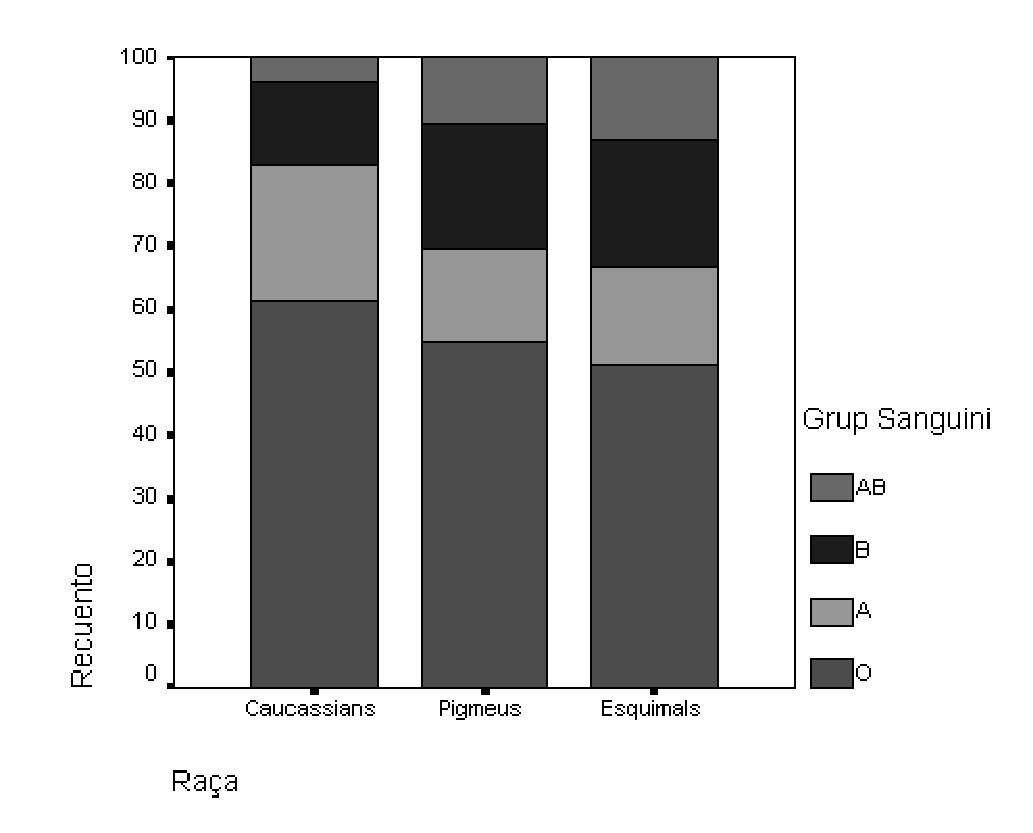
\includegraphics{./imatges/TestHomog.eps}
\end{center}
\caption{Diagrama de barres m\'{u}ltiples que mostra com es
distribueixen els grups sanguinis entre cada
ra\c{c}a}\label{testhomog}
\end{figure}

\chapter{Estad�stica no param�trica}
\label{capitol-No-Parametrica}

\section{Introducci�}

En aquest cap�tol presentarem de forma breu alguns tests no
param�trics per a problemes d'una, dues o v�ries mostres.
L'objectiu d'aquests tests �s disposar d'alternatives a les proves
d'hip�tesis de comparaci� cl�ssiques quan no es coneix la forma de
la distribuci� de les dades o la llei de les variables. En
particular seran alternatives als tests sobre la mitjana o
comparaci� de mitjanes quan no es verifica la suposici� de
normalitat de les dades. Ens referim als tests basats en
poblacions normals com a \emph{contrastos param�trics} ja que es
basen en comparar mitjanes o par�metres de la llei normal. En
contraposici�, els que considerem aqu� i que denominarem
\emph{contrastos no param�trics} poden comparar medianes, quantils
o fins i tot tota la distribuci� en bloc. Observem doncs que
\emph{no param�trics} no significa que aquests tests no compararin
algun par�metre com la mediana, m�s aviat significa que no volem
fer determinades suposicions sobre la funci� de distribuci� de les
variables.

Des d'un punt de vista pr�ctic, que tamb� �s el que adopten molts
programes informatics d'an�lisi estad�stica, distingirem entre:

\begin{itemize}
\item  Problemes d'una mostra

\item  Problemes de dues mostres amb dades aparellades

\item  Problemes de dues mostres independents

\item  Problemes de $k$ mostres independents.
\end{itemize}

Aquesta distinci� ens permet classificar les t�cniques que
estudiem i comparar-les amb les corresponents proves
param�triques:
\begin{center}
\begin{tabular}{|l|l|l|}
\hline \textbf{Problema} & \textbf{Test param�tric} & \textbf{Test no param�tric} \\ \hline
Una mostra & Test $t$ d'una mostra & Test dels signes \\
           &                       & Test dels rangs signats \\ \hline
Dades aparellades & Test $t$ de dades  & Test dels signes \\
                  & aparellades        & Test dels rangs signats \\ \hline
Dues mostres ind. & Test $t$ per a dues & Test $U$ de Mann-Whitney \\
                  & mostres ind. (amb  &  \\
                  & test $F$ previ)    &  \\ \hline
$k$ mostres ind. & ANOVA\ d'un factor & Test de Kruskal-Wallis \\
\hline
\end{tabular}
\end{center}

A m�s, alguns tests no param�trics tenen d'altres utilitats com
els tests d'aleatorietat, els tests de ratxes, etc

\section{Test dels signes}

\subsection{Test per a la mediana}
Sigui $X$ una variable aleat�ria amb distribuci� continua $F_X$
desconeguda i $M=Q_{50}$ la seva mediana o quantil 50\%, �s a dir,
el valor tal que
\[
P(X\leq M)=0.5
\]
Suposem que volem contrastar les hip�tesis
\[
\begin{split}
H_0 &: M=m_0 \\
H_1 &: M\ne m_0
\end{split}
\]

Donada una mostra $x_1,x_2,\dots,x_n$, considerem el ``signe'' de cada valor
mostral per comparaci� amb la mediana proposada per la hip�tesi $H_0$, �s a dir,
\[
\textrm{signe}(x_i)=\left\{
\begin{array}{ll}
+ & \textrm{si $x_i>m_0$} \\
- & \textrm{si $x_i<m_0$}
\end{array}
\right.
\]

L'estad�stic $B=\textrm{``Nombre de signes positius''}$ �s:
\[
B(x_1,x_2,\dots,x_n) =\sum_{i=1}^n I_{x_i>m_0}
\]
on
\[
I_{x_i>m_0}=\left\{
\begin{array}{ll}
1 & \textrm{si $x_i>m_0$ ($\textrm{signe}(x_i)=+$)} \\
0 & \textrm{si $x_i<m_0$ ($\textrm{signe}(x_i)=-$)}
\end{array}
\right.
\]

Si la hip�tesi nu{\ll}a �s certa la distribuci� de l'estad�stic
$B$ ser� una binomial de par�metres $n$ i $1/2$ i �s raonable
esperar que $B$ prengui valors pr�xims a $n/2$, mentre que quan
sigui falsa �s d'esperar que prengui valors a les cues de la
distribuci�. Aix� doncs, una regi� cr�tica per al test ser�
aquella en que el nombre de signes positius sigui massa alt o
massa baix com per ser coherent amb la hip�tesi nu{\ll}a que
implica que n'hi ha tants de positius com negatius. Podem agafar
com regi� cr�tica:
\[
W =\{B(\mathbf{x})\leq b_{\alpha/2}\}\cup \{B(\mathbf{x})\geq
b_{1-\alpha/2}\}
\]
on $b_{\alpha/2}$ i $b_{1-\alpha/2}$ es determinen de forma que la
probabilitat de les dues cues d'una distribuci� $B(n,\frac 12)$
sigui igual al nivell de significaci� $\alpha$ (o una mica menor
que $\alpha$), �s a dir,
\[
\sum_{i=0}^{b_{\alpha/2}}\binom ni\left( \frac 12\right)^i \left(
\frac 12\right)^{n-i}+ \sum_{i=b_{1-\alpha/2}}^n\binom ni\left(
\frac 12\right)^i \left( \frac 12\right)^{n-i}\leq \alpha
\]

\textbf{Observacions}

\begin{itemize}
\item Encara que amb probabilitat te�rica zero, perqu� la variable
considerada t� funci� de distribuci� continua, es pot donar el cas
$x_i=m_0$ de signe indefinit. Si no �s possible augmentar la
precisi�, s'aconsella eliminar aquest valor mostral i
descomptar-ho conseq�entment de la mida de la mostra.

\item  Si la hip�tesi alternativa �s $M<m_0$ o b� $M>m_0$
la regi� cr�tica s'adapta a aquesta hip�tesi de la manera
raonable, �s a dir:
\[
\begin{split}
H_1 &: M<m_0 \quad\Rightarrow\quad
W=\left\{B(\mathbf{x})\leq b_{\alpha}\right\} \\
H_1 &: M>m_0 \quad\Rightarrow\quad
W=\left\{B(\mathbf{x})\geq b_{1-\alpha/2}\right\}
\end{split}
\]

\item  Alguns llibres porten taules de la distribuci� binomial que podem
fer servir per trobar els valors cr�tics. Per a $n\geq 20$ podem
aproximar la binomial per una normal.
\end{itemize}

\begin{example}\label{example_nopara_1}
La seg�ent taula recull una mostra de 40 notes en un examen.
Contrasteu amb un nivell de significaci� 0.05 la hip�tesi que el
valor mitj� (mediana) de les notes �s 66.
\[
\begin{array}{|cccccccccc|} \hline
  % after \\: \hline or \cline{col1-col2} \cline{col3-col4} ...
  71 & 67 & 55 & 64 & 82 & 66 & 74 & 58 & 79 & 61 \\
  78 & 46 & 84 & 93 & 72 & 54 & 78 & 86 & 48 & 52 \\
  67 & 95 & 70 & 43 & 70 & 73 & 57 & 64 & 60 & 83 \\
  73 & 40 & 78 & 70 & 64 & 86 & 76 & 62 & 95 & 66 \\ \hline
  + & + & - & - & + & 0 & + & - & + & - \\
  + & - & + & + & + & - & + & + & - & - \\
  + & + & + & - & + & + & - & - & - & + \\
  + & - & + & + & - & + & + & - & + & 0 \\ \hline
\end{array}
\]
\end{example}

\textit{Soluci�:}

Si restem 66 de les notes observades i retenim nom�s els signes de
les difer�ncies, s'obtenen 23 signes $+$, 15 signes $-$ i 2 zeros.
Descartats els zeros, $B=23$ sobre un total de $38$. Si fem un
contrast bilateral amb l'aproximaci� normal, la regi� d'acceptaci�
�s $\{-1.96\le z\le 1.96\}$.

Donat que
\[
z=\frac{(23-0.5)-38\cdot 0.5}{\sqrt{38\cdot 0.5\cdot 0.5}}=1.14
\]
acceptem la hip�tesi que la mediana �s 66, al nivell 0.05.


\subsection{Test dels signes per a dades aparellades}

El test dels signes pot servir tamb� en el cas de dades
aparellades. \par
Considerem una mostra de dues variables $X,Y$
\[
(x_1,y_1),(x_2,y_2),\dots,(x_n,y_n)
\]
amb $n$ observacions en dues situacions el m�s homog�nies
possible.

Suposem que les distribucions de les dues variables s�n semblants,
excepte potser en un par�metre de localitzaci� com la mediana. �s
a dir, les dues situacions considerades nom�s poden traslladar la
distribuci� i no modifiquen la forma.

Ara volem contrastar la hip�tesi que no hi ha difer�ncia entre les
dues situacions: les difer�ncies observades entre els valors $x_i$
i $y_i$ s�n degudes a l'atzar, �s a dir, les dues mostres
$x_1,\dots,x_n$ i $y_1,\dots,y_n$ procedeixen de la mateixa
poblaci�. Aix� es pot expressar estad�sticament amb la hip�tesi
$H_0$ d'igualtat de les distribucions de probabilitat, que amb les
suposicions assumides �s equivalent a la igualtat de medianes.

Si la hip�tesi $H_0$ �s certa, i la distribuci� de la variable
difer�ncia $D=X-Y$ �s sim�trica en l'origen, es verificar�
\[
P(X>Y)=P(X-Y>0)=\frac 12
\]
Aix� doncs, podem aplicar el test dels signes a la variable
difer�ncia $D=X-Y$. En general, per� no necess�riament sempre, s'agafar�
com valor de $m_0$ el 0.

\begin{example}\label{example_nopara_2}
Es vol comparar el n�mero de peces defectuoses produ�des per dues
m�quines diferents. S'observa la producci� en 10 dies, amb la
mateixa producci� di�ria per a les dues m�quines encara que
diferent cada dia, i els resultats s�n:
\[
\begin{array}{|l|cccccccccc|}\hline
\textrm{{\em Dia}} & 1 & 2 & 3 & 4 & 5 & 6 & 7 & 8 & 9 & 10 \\
\hline \textrm{{\em M�quina 1}} & 46 & 110 & 70 & 54 & 60 & 120 &
82 & 76 & 37 & 28 \\ \hline
\textrm{{\em M�quina 2}} & 42 & 87 & 75 & 50 & 48 & 108 & 80 & 67 & 40 & 25 \\
\hline
\end{array}
\]
Amb un nivell de significaci� $\alpha=0.06$, podem acceptar que la
primera m�quina produeix m�s peces defectuoses?
\end{example}

\textit{Soluci�:}

El fet que la producci� total di�ria d'ambdues m�quines sigui la
mateixa permet considerar les dades aparellades. Que la producci�
di�ria sigui diferent cada dia aconsella utilitzar un test no
param�tric. \par Observem els signes de les difer�ncies
\[
\begin{array}{lcccccccccc}
\textrm{Dia:} & 1 & 2 & 3 & 4 & 5 & 6 & 7 & 8 & 9 & 10 \\
\textrm{Signe:} & + & + & - & + & + & + & + & + & - & +
\end{array}
\]
De manera que $B=8$ sobre $n=10$. En aquest contrast, la regi�
cr�tica �s unilateral i concretament �s $W=\{8,9,10\}$, ja que
\[
P(B\ge 8)=\sum_{i=8}^{10} \binom{10}{i} 0.5^{10} = 0.0547 <
\alpha=0.06
\]
Donat que la freq��ncia observada �s 8 i pertany a la regi�
cr�tica, rebutgem la igualtat i podem acceptar que la m�quina 1
produeix m�s peces defectuoses.

\subsection{Test per a dades binaries}

En el cas d'una mostra de valors d'una variable dicot�mica com per
exemple
\[
a,a,b,b,b,a,a,b,a,\dots,b
\]
podem aplicar el test dels signes per contrastar l'equilibri de
les probabilitats d'ambd�s valors.

\begin{example}\label{example_nopara_3}
Davant d'un canvi en un servei p�blic es fa una enquesta a 300
persones, a les quals se'ls demana si el servei ha millorat o
empitjorat, sense possibilitat de ser indiferent. Ha resultat que
197 persones han dit que el servei ha millorat i volem contrastar
aquest fet amb un nivell de significaci� del 0.01.
\end{example}

\textit{Soluci�:}

Sota la hip�tesi nu{\ll}a d'equilibri, el n�mero $B$ de persones
que afirmen que el servei ha millorat segueix una distribuci�
binomial $B(300,0.5)$ de forma que
\[
z=\frac{(197-0.5)-150}{\sqrt{300\cdot 0.5\cdot 0.5}}=5.37
\]
La regi� cr�tica d'una cua �s $W=\{z>2.33\}$ per a un
$\alpha=0.01$, de manera que acceptem l'opini� que el servei ha
millorat.

\subsection{Test de McNemar}

�s una variant del test dels signes. Suposem que un conjunt
d'individus es classifiquen en dues categories oposades, que podem
indicar amb els signes $+$ i $-$. Despr�s d'algun est�mul, �s
possible que alguns individus canvi�n de categoria, de forma que
s'obt� la taula de freq��ncies
\begin{center}
\begin{tabular}{lc|cc|}
 & & \multicolumn{2}{c|}{Despr�s} \\
 & & $-$ & $+$ \\ \hline
 Abans & $+$ & $a$ & $b$ \\
 & $-$ & $c$ & $d$ \\ \hline
\end{tabular}
\qquad $a+b+c+d=n$
\end{center}
Nom�s $a+d$ individus han canviat. Sota la hip�tesi nu{\ll}a que
les proporcions no canvien, les probabilitats s�n
\[
P(+\to -)=P(-\to +)=1/2
\]
de manera que la freq��ncia esperada en aquest dos casos �s
$(a+d)/2$. Podem aplicar el test khi-quadrat
\[
\chi^2=\frac{(a-(a+d)/2)^2}{(a+d)/2}+\frac{(d-(a+d)/2)^2}{(a+d)/2}
=\frac{(a-d)^2}{a+d}\qquad\textrm{amb 1 g.ll.}
\]
Rebutjarem la hip�tesi d'equilibri si $\chi>\chi^2_{\alpha}$, on
$\alpha$ �s el nivell de significaci�. Si les freq��ncies s�n
petites �s convenient utilitzar la correcci� de Yates
\[
\chi=\frac{(|a-d|-1)^2}{a+d}
\]

\section{Test dels rangs amb signe de Wilcoxon}

Vist com extensi� de l'anterior test dels signes, la idea d'aquest
test �s fer servir, a m�s del signe, la magnitud de les
difer�ncies.

El \emph{rang} d'una observaci� �s la posici� que aquesta ocupa en
la mostra ordenada. Per exemple, si considerem la mostra
\[
x_1=3\quad x_2=0\quad x_3=5\quad x_4=1.9
\]
la mostra ordenada �s
\[
x_{(1)}=0\quad x_{(2)}=1.9\quad x_{(3)}=3\quad x_{(4)}=5
\]
de manera que els rangs valen:
\[
r(0)=1\quad r(1.9)=2\quad r(3)=3\quad r(5)=4
\]

Una part important de l'estad�stica no param�trica ha sorgit de la
substituci� dels valors quantitatius de les mostres pels seus
rangs i l'obtenci� d'estad�stics de test an�legs als utilitzats
amb dades quantitatives com, per exemple, un test equivalent al
test $t$ de Student per� basat en rangs o un coeficient de
correlaci� amb la mateixa f�rmula que el de Pearson per� fent
servir rangs.

Suposem que la hip�tesi nu{\ll}a �s la mateixa que en el test de
la mediana, �s a dir:
\[
\begin{split}
H_0 &: M=m_0 \\
H_1 &: M\neq m_0
\end{split}
\]
on $M$ representa la mediana d'una variable o, sovint, de la
difer�ncia entre dues variables aparellades.

Wilcoxon propos� considerar els estad�stics:
\[
\begin{split}
T^{+} &= \text{Suma dels rangs de les observacions amb signe $+$} \\
T^{-} &= \text{Suma dels rangs de les observacions amb signe $-$}
\end{split}
\]
\[
T^{+}=\sum_{i=1}^n r(|x_i-m_0|)I_{x_i>m_0}
\]

Si $H_0$ �s certa, llavors esperem que $T^{+}=T^{-}$.

L'estad�stic $T^{+}$ es coneix amb el nom d'estad�stic de Wilcoxon
i est� tabulat de forma que podem trobar uns valors $t_{\alpha/2}$
i  $t_{1-\alpha/2}$ tals que
\[
P[T^{+}< t_{\alpha/2}|H_0]+P[T^{+}> t_{1-\alpha/2}|H_0] \leq
\alpha
\]
i definir la regi� cr�tica com
\[
W =\{T^{+}<t_{\alpha/2}\}\cup \{T^{+}>t_{1-\alpha/2}\}
\]

\subsubsection{Observacions}

\begin{itemize}
\item  Per a valors grans de $n$ es pot fer servir el fet que, sota
$H_0$, l'estad�stic $T^{+}$ �s assimpt�ticament normal:
\[
T^{+}\sim AN(\mu_{T^{+}},\sigma_{T^{+}}),\quad
\mu_{T^{+}}=\frac{n(n+1)}4,\quad
\sigma_{T^{+}}^2=\frac{n(n+1)(2n+1)}{24}
\]
i per tant per mostres grans podem basar-nos en l'estad�stic
\[
Z=\frac{T^{+}-n(n+1)/4}{\sqrt{n(n+1)(2n+1)/24}}\sim N(0,1).
\]

\item  Una alternativa a l'estad�stic de test anterior �s considerar
l'estad�stic
\[
T=\textrm{m�n}(T^{+},T^{-}).
\]
Si $H_0$ �s certa, llavors $T^{+}=T^{-}$. Si no �s certa, tindrem
$T^{+}>T^{-}$ o b� $T^{+}<T^{-}$, de forma que el m�nim ser� un
valor ``petit''. El test basat en aquest estad�stic rebutjar� la
hip�tesi nu{\ll}a si $T$ �s m�s petit que $T_{^\alpha}$ on aquest
valor cr�tic s'obt� d'una taula diferent de la taula de valors
cr�tics per a $T^{+}$.
\end{itemize}

\begin{example}\label{example_nopara_4}
Donat que en l'exemple \ref{example_nopara_1} les notes s�n
num�riques podem utilitzar el test dels rangs amb signe per
contrastar si $H_0:M=66$ en front de $H_1:M\ne 66$ amb un nivell
de significaci� del 0.05.
\end{example}

\textit{Soluci�:}

\begin{table}[h]\label{taula_excel}
\begin{center}
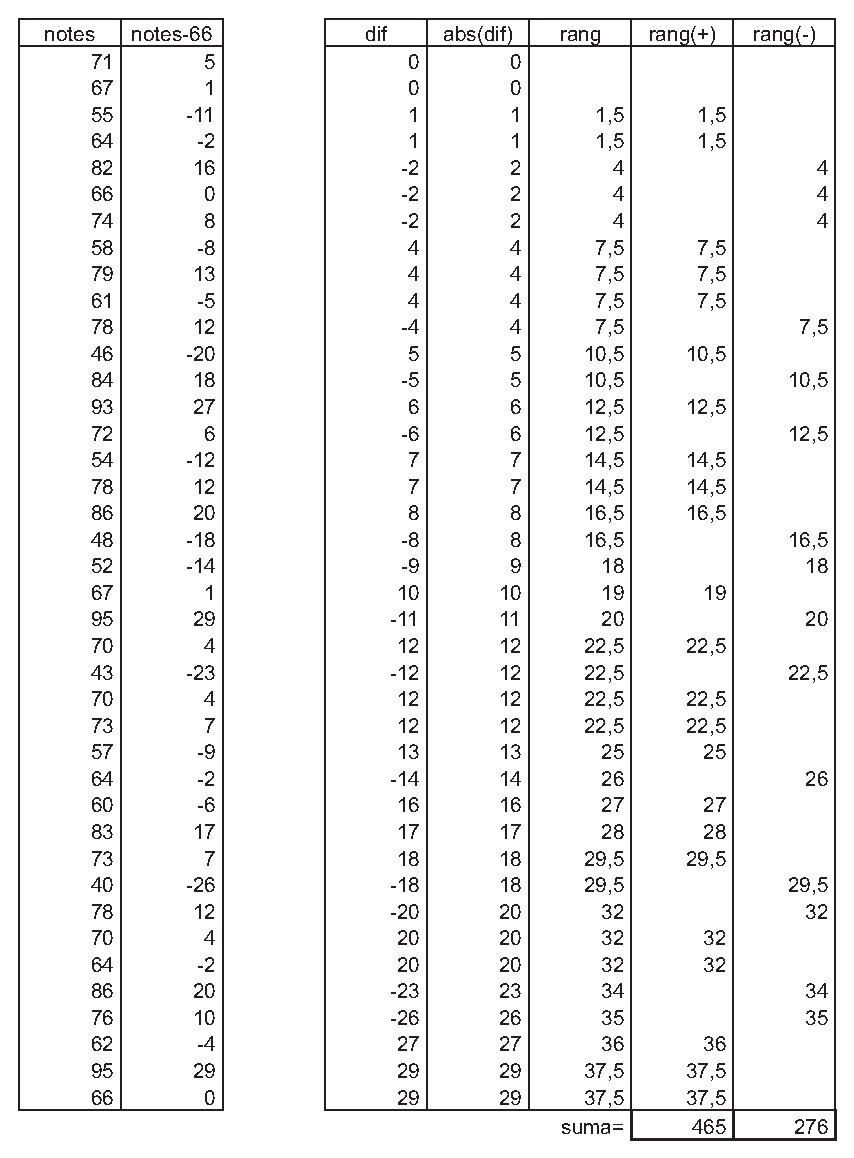
\includegraphics[width=9.6cm]{./imatges/tabla.eps}
\end{center}
\caption{Taula per a la suma dels rangs de l'exemple \ref{example_nopara_4}}
\end{table}

Per calcular l'estad�stic $T^{+}$ hem d'assignar els rangs
corresponents als valors positius de les difer�ncies entre les
observacions i el valor 66  proposat a la hip�tesi nu{\ll}a. Aix�
es fa de forma relativament simple amb un full de c�lcul com
EXCEL. En la taula 8.1 podem observar l'ordenaci� que es fa en
funci� dels valors absoluts de les difer�ncies. Observem tamb� que
cal repartir els rangs quan hi ha empats i que els dos zeros
queden exclosos.

El resultat �s que $T^{+}=465$ amb un $n=38$, de manera que
\[
z=\frac{465-(38\cdot 39)/4}{\sqrt{(38\cdot 39\cdot 77)/24}}=1.37
\]
que queda dins de la regi� d'acceptaci� $\{-1.96\le z\le 1.96\}$.

\begin{example}\label{example_nopara_5}
Donat que en l'exemple \ref{example_nopara_2} les observacions s�n
num�riques i aparellades, podem utilitzar els valors de les
difer�ncies amb el test dels rangs amb signe per contrastar si hi
ha difer�ncies entre les dues m�quines.
\end{example}

\textit{Soluci�:}
\begin{table}[h]\label{taula_excel2}
\begin{center}
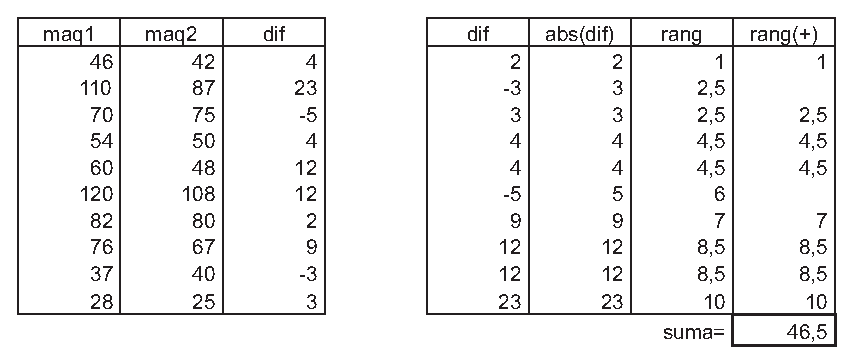
\includegraphics[width=9.6cm]{./imatges/tabla2.eps}
\end{center}
\caption{Taula per a la suma dels rangs de l'exemple
\ref{example_nopara_5}}
\end{table}

Primer calculem les difer�ncies i les ordenem pel seu valor
absolut (veure la taula 8.2). En aquest cas hi ha molts empats i
s'han de repartir els rangs. L'estad�stic $T^{+}$ �s $46.5$ amb un
$n=10$, un valor clarament superior a l'esperat si $H_0$ �s certa.

Amb un nivell de significaci� de 0.05, la regi� cr�tica que s'obt�
a la taula de Wilcoxon �s $\{T^{+}>44\}$, de forma que rebutgem
$H_0$ i admetem que la primera m�quina fabrica m�s peces
defectuoses.

\section{El test $U$ de Mann-Whitney}

Aquest test permet comparar dues poblacions amb mostres
independents.

Suposem que obtenim dues mostres independents
\[
(x_1,...,x_{n_1}),(y_1,...,y_{n_2})
\]
de dues poblacions $X,Y$ amb funcions de distribuci� $F_X,F_Y$
respectivament. Volem contrastar la hip�tesi $H_0 : F_X=F_Y$ front
alguna de les alternatives
\[
H_1 : F_X\neq F_Y\qquad H_1:F_X<F_Y \qquad H_1:F_X>F_Y
\]

Si la hip�tesi nu{\ll}a �s certa, llavors $P(X<Y)=\frac 12$. A
m�s, com hi ha $n_1\cdot n_2$ parelles possibles, el nombre de
parelles d'observacions $(x_i,y_j)$ que esperem que verifiquin
$x_i<y_j$ estar� al voltant de $\frac{n_1\cdot n_2}2$.

Un estad�stic de test raonable per decidir si acceptem o rebutgem
la hip�tesi nu{\ll}a �s el nombre de parelles que verifiquen
$x_i<y_j$ que definim com:
\[
U=\sum_{i=1}^{n_1}\sum_{j=1}^{n_2}I_{x_i<y_j}
\]

Una desviaci� significativa de $U$ respecte al valor esperat
$\frac{n_1\cdot n_2}2$ far� rebutjar la hip�tesi nu{\ll}a. Per
decidir si $U$ �s significatiu consultarem la taula de
Mann-Whitney-Wilcoxon que permet decidir si rebutgem $H_0$ en
funci� del nivell de significaci� escollit i de les mides mostrals
$n_1$ i $n_2$.

\subsubsection{Observacions}

\begin{itemize}
\item  Un procediment alternatiu per calcular $U$, i sovint m�s
c�mode, consisteix en formar la mostra conjunta, reunint les dues
individuals, i assignar els rangs $1,2,...,n_1+n_2$ a cadascun
dels valors de la mostra ordenada. Es pot calcular $U$ a partir de
la relaci�:
\[
U=W-\frac{n_2(n_2+1)}2
\]
on $W$ �s la suma dels rangs de les observacions $y_j$
\[
W=\sum_{j=1}^{n_2}r(y_j)
\]
Aquest estad�stic $W$ per comparar dues poblacions va ser proposat
per Wilcoxon per�, per la relaci� anterior, �s equivalent a
l'estad�stic $U$ de Mann-Whitney.

\item Si no hi ha ligadures o empats, la relaci� entre l'estad�stic de
Wilcoxon $W$ (suma de rangs corresponents a les observacions $Y$)
i l'estad�stic $U$ de Mann-Whitney (n�mero de vegades que
$x_i<y_j$ a la mostra conjunta ordenada) �s
\[
W=\frac{n_2(n_2+1)}{2}+U
\]
Si $W'$ �s la suma dels rangs corresponents a les observacions
$X$, llavors
\[
W+W'=\frac{(n_1+n_2)(n_1+n_2+1)}{2}
\]
De forma que si $U'$ �s el n�mero de vegades que $y_j<x_i$,
resulta
\[
U+U'=n_1n_2 \qquad W'=\frac{n_1(n_1+1)}{2}+U'
\]

\item  Donats $n_1,n_2$ ($n_1,n_2\leq 10$) la taula de
Mann-Whitney \footnote{Aix� dep�n dels autors i cal mirar amb cura
la definici� de cada taula} proporciona l'enter $a_p$ i la
probabilitat $p$ tal que
\[
P(U\leq a_p)=p
\]
Veiem com s'utilitzen aquests valors. \par En una prova unilateral
amb hip�tesi alternativa $H_1:F_X<F_Y$, el criteri de decisi� ser�
rebutjar la hip�tesi nu{\ll}a si $\{U\leq a_p\}$, on $p$ �s
l'aproximaci� per defecte del nivell de significaci�. Aix� �s
perqu�, si �s certa l'alternativa, llavors $F_X(s)\leq F_Y(s) \
\forall s$ i $F_X(s)< F_Y(s)$ per a algun $s$ (es diu que $X$ �s
estoc�sticament m�s gran que $Y$), el que implica que
$P(X>Y)>1/2$, de manera que �s probable que $U$ sigui petit.

L'estad�stic $U$ ha de verificar $U<n_1n_2/2$, en cas contrari
s'utilitza
\[
U'=n_1n_2-U
\]
i la regla �s la mateixa, per� fent servir $U'$.

Si l'alternativa �s $H_1:F_X>F_Y$, podem intercanviar $X$ i $Y$.

En una prova bilateral es buscar� $a_{p/2}$ de forma que $P(U\leq
a_{p/2})=p/2$, on $p$ �s l'aproximaci� per defecte del nivell de
significaci�, i la regi� de rebuig �s
\[
\{U\leq a_{p/2}\}\cup\{U'\leq a_{p/2}\}
\]

\item  Per a mostres ``grans'' es pot fer servir el fet que, sota
$H_0$, l'estad�stic $U$ �s assimpt�ticament normal:
\[
U\sim AN(\mu_U,\sigma_U),\quad\mu_U=\frac{n_1n_2}2, \quad
\sigma_U^2=\frac{n_1n_2(n_1+n_2+1)}{12}
\]
i per tant, per a $n_1>10$ o $n_2>10$ podem basar-nos en un
estad�stic de test
\[
Z=\dfrac{U-n_1n_2/2}{\sqrt{n_1n_2(n_1+n_2+1)/12}}\sim N(0,1)
\]
\end{itemize}

\begin{example}\label{example_nopara_6}
Per tal de comparar la resist�ncia en kg/cm$^2$ d'un material
subministrat per dos prove�dors es van mesurar dues mostres d'uns
quants elements:
\begin{center}
\begin{tabular}{ll}
 Prove�dor A & 202, 229, 215, 220, 223, 233, 208, 228, 209 \\
 Prove�dor B & 221, 207, 185, 203, 187, 190, 195, 204, 212
\end{tabular}
\end{center}
Amb un nivell de significaci� del 0.05, indiqueu si hi ha
difer�ncies entre els materials subministrats pels dos prove�dors.
\end{example}

\textit{Soluci�:}
\begin{table}[h]\label{taula_excel3}
\begin{center}
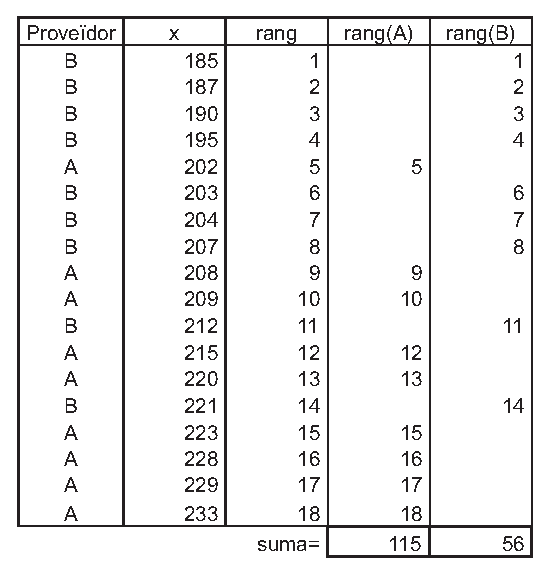
\includegraphics[width=6cm]{./imatges/tabla3.eps}
\end{center}
\caption{Taula per a la suma dels rangs de l'exemple
\ref{example_nopara_6}}
\end{table}

�s clar que es tracta de comparar dues mostres independents i que
el fet que $n_1=n_2=9$ no �s important. La taula 8.3 indica el
c�lcul de les sumes de rangs per a cada mostra, de forma que
\[
W=56 \qquad W'=115 \qquad W+W'=171=\frac{(9+9)(9+9+1)}{2}
\]
d'on s'obt�
\[
U=W-\frac{9\cdot 10}{2}=56-45=11<\frac{n_1n_2}{2}=40.5
\]
La regi� cr�tica per $n_1=n_2=9$ i $\alpha=0.05$ �s $\{U\le 22\}$,
de manera que el valor observat $U=11$ cau en ella i implica el
rebuig de l'equival�ncia de les dades.

\section{Comparaci� de medianes}

Considerem una situaci� en la que es vol comparar dues poblacions
continues amb distribucions d'igual forma i tractar de detectar
despla�aments entre ambdues distribucions.

Siguin $x_1,\dots,x_{n_1}$ i $y_1,\dots,y_{n_2}$ dues mostres
aleat�ries corresponents a cada poblaci� i independents entre s�.
Si s'ordenen conjuntament les dues mostres en ordre creixent i es
considera la mediana $M$ de la mostra combinada, podem calcular
l'estad�stic
\[
T=\sum_{i=1}^{n_1} I_{x_i<M}
\]
que serveix per contrastar la hip�tesis $H_0:M_X=M_Y$.

Si ambdues poblacions tenen la mateixa distribuci�, �s d'esperar
que $T$ sigui pr�xim a $n_1/2$. En canvi, si $T$ resulta molt m�s
gran que $n_1/2$, �s raonable suposar que la mediana $M_X$ de la
primera poblaci� �s inferior a la de la segona $M_Y$; mentre que
si $T$ �s molt menor que $n_1/2$, aix� sembla indicar que $M_X$ �s
superior a $M_Y$. Les regions cr�tiques s�n:

\medskip
\begin{center}
\begin{tabular}{ll}
\hline \textbf{Alternativa} & \textbf{Regi� cr�tica} \\ \hline
$M_X<M_Y$ & $\{T\geq k\}$ \\
$M_X>M_Y$ & $\{T\leq k'\}$ \\
$M_X\neq M_Y$ & $\{T\leq k_1\}\cup\{T\geq k_2\}$
\\ \hline
\end{tabular}
\end{center}
\medskip

Si la distribuci� d'ambdues poblacions �s la mateixa, la
distribuci� de $T$ es pot trobar amb facilitat. Donat que les
$n_1+n_2$ observacions s�n independents i igualment distribu�des,
les $\binom{n_1+n_2}{n_1}$ maneres d'assignar $n_1$ a la primera
mostra (i les altres $n_2$ a la segona) s�n equiprobables. Si $p$
�s la part sencera de $(n_1+n_2)/2$, hi ha $p$ de les $n_1+n_2$
observacions inferiors a $M$ i ser� $T=t$ en totes les
assignacions en les que resultin $t$ de la primera mostra d'entre
les $p$ primeres i $n_1-t$ entre les $n_1+n_2-p$ �ltimes. Aix�
\[
P(T=t)=\frac{\displaystyle\binom{p}{t}\binom{n_1+n_2-p}{n_1-t}}{%
\displaystyle\binom{n_1+n_2}{n_1}}
\]
on $t$ pot variar entre $\max\{0,p-n_2\}$ i $\min\{n_1,p\}$. Es
tracta doncs d'una distribuci� hipergeom�trica que pot
aproximar-se, si $n_1$ i $n_2$ s�n grans, per una
$N(n_1/2,\sqrt{n_1n_2/4(n_1+n_2)})$.

\begin{example}\label{example_nopara_7}
Amb les dades de l'exemple \ref{example_nopara_6}, calculeu
l'estad�stic $T$ i compareu les medianes de les dues mostres.
\end{example}

\textit{Soluci�:}

La mediana conjunta �s $M=208.5$, de manera que �s evident que
$T=2$. Els c�lculs per a una distribuci� hipergeom�trica amb
$n_1=n_2=9$ i $p=9$ ens proporcionen
\[
P(T\le 2)=P(T\ge 7)=0.02834
\]
Unes cues que sumen una mica m�s del 0.05. El valor observat $T=2$
cau a la regi� cr�tica i, en conseq��ncia, rebutgem la igualtat de
medianes.

\bigskip
Un procediment alternatiu es pot aplicar amb el test
khi-quadrat.
\par Considerem la mediana $M$ de tots els valors mostrals
conjuntament i dividim cada mostra original en dos grups: aquells
que prenen valors inferiors o iguals a la mediana i els que prenen
valors superiors.

S'obtenen aix� quatre classes d'efectius com es recull en la
taula:
\begin{center}
\begin{tabular}{|l|c|c|c|}
\hline
& Grup I & Grup II & \\ \hline
Observacions amb & & & \\
valors inferiors & $n_{11}$ & $n_{12}$ & $n_{1\bullet}$ \\
a la mediana & & & \\ \hline
Observacions amb & & & \\
valors superiors & $n_{21}$ & $n_{22}$ & $n_{2\bullet}$ \\
a la mediana & & & \\ \hline
Total & $n_{\bullet 1}=n_1$ & $n_{\bullet 2}=n_2$ & \\ \hline
\end{tabular}
\end{center}
Es calcula l'estad�stic $\chi^2$ ja que es tracta d'una comparaci�
de proporcions o test d'homogene�tat en una taula $2\times 2$. La
regi� cr�tica es determina a partir de la distribuci� khi-quadrat
o les alternatives estudiades.

\begin{example}\label{example_nopara_8}
Amb les dades de l'exemple \ref{example_nopara_6}, calculeu
l'estad�stic $\chi^2$ i compareu les medianes de les dues mostres.
\end{example}

\textit{Soluci�:}

Com ja sabem, la mediana comuna de les dues mostres �s $M=208.5$.
Llavors la taula pel test d'homogene�tat resulta
\begin{center}
\begin{tabular}{|l|c|c|c|}
\hline & Pro. A & Pro. B & \\ \hline
valors inferiors & 2 & 7 & 9 \\
valors superiors & 7 & 2 & 9 \\
\hline Total & 9 & 9 &
\\ \hline
\end{tabular}
\end{center}
Aix� hem de calcular l'estad�stic khi-quadrat amb la correcci� de
Yates
\[
\chi^2=\frac{(|2\cdot 2-7\cdot 7|-18/2)^2}{9\cdot 9\cdot 9\cdot
9}18=3.556
\]
Amb un grau de llibertat i per un nivell de significaci� del 0.05,
la regi� cr�tica comen�a en $\chi^2_{0.05}=3.841$, de forma que
podem acceptar la hip�tesi nu{\ll}a.

\bigskip
Amb mides mostrals grans, el test khi-quadrat �s preferible si no
hi ha const�ncia que la forma d'ambdues distribucions sigui la
mateixa, ja que el test $T$ anterior t� tend�ncia a acceptar la
homogene�tat si $M_X=M_Y$ encara que la forma de les distribucions
sigui diferent.

Per la mateixa ra� es preferible el test de Kolmogorov-Smirnov que
expliquem a la seg�ent secci�.

% De fet, l'estad�stic $T$ equival a calcular la difer�ncia...

\section{Test de Kolmogorov-Smirnov per a l'homogene�tat}

Quan disposem de dues mostres independents $x_1,x_2,\dots,x_{n_1}$
i $y_1,y_2,\dots,y_{n_2}$ de dues poblacions amb distribucions
desconegudes $F_X$ i $F_Y$ respectivament i volem contrastar la
seva coincid�ncia, �s a dir, la hip�tesi $H_0:F_X=F_Y$ podem
comparar les distribucions emp�riques associades a cada mostra.
Aix� �s possible si coneixem els valors exactes de les
observacions i, en aquest aspecte, �s millor aquesta comparaci�
que el test khi-quadrat d'homogene�tat que utilitza freq��ncies i
necessita moltes dades de cada poblaci�.

Les distribucions emp�riques s�n:
\[
F_{n_1}(z)=\frac{1}{n_1}\sum_{i=1}^{n_1}I_{x_i<z} \qquad
G_{n_2}(z)=\frac{1}{n_2}\sum_{i=1}^{n_2}I_{y_i<z}
\]
i l'estad�stic de Kolmogorov-Smirnov
\[
\Delta_{n_1,n_2}=\sup_{z\in\mathbb{R}}|F_{n_1}(z)-G_{n_2}(z)|
\]
Si la hip�tesi $H_0$ �s certa, les dues distribucions emp�riques
han d'estar molt pr�ximes i la mesura global de discrep�ncia
$\Delta_{n_1,n_2}$ ser� petita. Pel contrari, quan $F_X\ne F_Y$ el
valor de $\Delta_{n_1,n_2}$ ser� m�s gran, de manera que la regi�
cr�tica que hem de considerar �s de la forma
\[
\{\Delta_{n_1,n_2}> a\}
\]

El test es basa en el Teorema de Smirnov.
\begin{teorema}
Si les distribucions continues de les dues poblacions coincideixen
$F_X=F_Y$ i $n_1\to\infty,n_2\to\infty$, llavors per a cada
$\lambda$
\[
P\left(\sqrt{\frac{n_1n_2}{n_1+n_2}}\Delta_{n_1,n_2}\le\lambda\right)\to
Q(\lambda)=\sum_{i=-\infty}^{\infty} (-1)^i e^{-2i^2\lambda^2}
\]
on $Q(\lambda)$ �s la distribuci� asimpt�tica de
Kolmogorov-Smirnov.
\end{teorema}
Per aplicar aquest resultat, primer determinarem a la taula de
Kolmogorov-Smirnov el valor tal que
$Q(\lambda_{\alpha})=1-\alpha$, on $\alpha$ �s el nivell de
significaci�. Llavors, tot suposant que $n_1$ i $n_2$ s�n grans,
acceptarem $H_0$ si
\[
\sqrt{\frac{n_1n_2}{n_1+n_2}}\Delta_{n_1,n_2}\le\lambda_{\alpha}
\]
i rebutjarem $H_0$ en cas contrari.

Per a valors petits de $n_1$ i $n_2$ existeixen unes taules
calculades per Massey que proporcionen els valors cr�tics
$a_{\alpha}$, de forma que rebutgem $H_0$ si $\Delta_{n_1,n_2}>
a_{\alpha}$. Alguns llibres porten exclusivament la taula en el
cas $n_1=n_2$.

\begin{example}\label{example_nopara_9}
Amb les dades de l'exemple \ref{example_nopara_6}, calculeu
l'estad�stic de Kolmogorov-Smirnov i compareu les distribucions de
les dues mostres.
\end{example}

\textit{Soluci�:}
\begin{table}[h]\label{taula_excel4}
\begin{center}
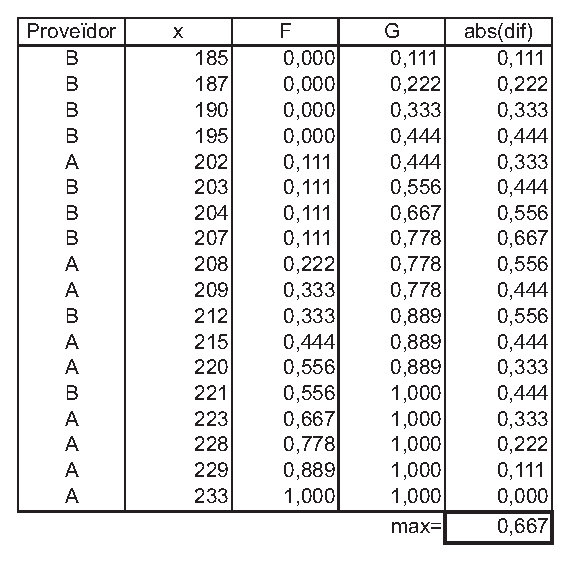
\includegraphics[width=6cm]{./imatges/tabla4.eps}
\end{center}
\caption{Taula per calcular $\Delta$ amb les dades de l'exemple
\ref{example_nopara_6}}
\end{table}

A la taula 8.4 %\ref{taula_excel4}
veiem els c�lculs fets amb un
full EXCEL. Observem els increments de les freq��ncies a ra� de
$1/9$.

L'estad�stic �s $\Delta=0.667$ i cau justament a la frontera de la
regi� cr�tica $\Delta_{9,9}> 0.667$ de la taula de Massey pel
nivell de significaci� 0.05 i $n_1=n_2=9$.

\section{Test $H$ de Kruskal-Wallis}

El test $U$ �s un test no param�tric per decidir si dues mostres
independents provenen o no de la mateixa poblaci�. El test $H$ de
Kruskal-Wallis �s una generalitzaci� per a $k$ mostres agafades en
$k$ poblacions. Aix� doncs, �s una versi� no param�trica d'un
ANOVA d'un factor.

Considerem $k$ mostres de mides $n_1,n_2,\dots,n_k$ recollides en
les $k$ poblacions i tals que $n_1+n_2+\cdots+n_k=n$. Suposem que
ordenem totes les observacions de forma conjunta i calculem les
sumes dels rangs per a les $k$ mostres $R_1,R_2,\dots,R_k$,
respectivament. Si definim l'estad�stic
\[
H=\left(\frac{12}{n(n+1)}\sum_{i=1}^k \frac{R_i^2}{n_i}\right)
-3(n+1)
\]
es demostra que, si existeix homogene�tat entre les distribucions
dels $k$ grups, la seva distribuci� en el mostratge est� molt
pr�xima a una khi-quadrat amb $k-1$ graus de llibertat quan les
mides mostrals $n_i$ s�n grans. Aix�, exigirem sempre que
$n_1,n_2,\dots,n_k$ siguin tots ells superiors a 5. Per a valors
petits �s necessari consultar unes taules especials.

\subsubsection{Observacions}

\begin{itemize}
\item L'estad�stic de Kruskal-Wallis es pot posar en la forma
\[
H=\frac{12}{n(n+1)}\sum_{i=1}^k n_i(R_{\bullet i}-R_{\bullet\bullet})^2
\]
on $R_{\bullet i}=R_i/n_i$, $R_{\bullet\bullet}=(n+1)/2$.
D'aquesta forma, el test basat en $H$ si sembla molt al test $F$
en un disseny d'un factor i r�pliques.

\item Si existeixen observacions repetides, l'estad�stic $H$ es
corregeix amb un factor de manera que el nou estad�stic �s
\[
H'=\frac{H}{1-\frac{\sum_{j=1}^r (t_j^3-t_j)}{n^3-n}}
\]
on $t_j$ �s el n�mero d'observacions en la mostra combinada
repetides per a un rang donat i $r$ el n�mero de repeticions.
Aquesta correcci� no t� molt d'efecte sobre el valor de $H$, fins
i tot en pres�ncia de moltes observacions repetides.
\end{itemize}

\begin{example}\label{example_nopara_10}
Es vol comparar el pes en grams d'un producte envasat per tres
fabricants amb mostres de mida 6 en els tres casos.
\begin{center}
\begin{tabular}{lcccccc}
Fabr. A & 251 & 250 & 249 & 255 & 258 & 258 \\
Fabr. B & 247 & 246 & 250 & 241 & 240 & 242 \\
Fabr. C & 228 & 236 & 240 & 225 & 236 & 230
\end{tabular}
\end{center}
Estudieu si hi ha difer�ncies entre els tres fabricants amb el
test de Kruskal-Wallis.
\end{example}

\textit{Soluci�:}
\begin{table}[h]\label{taula_excel5}
\begin{center}
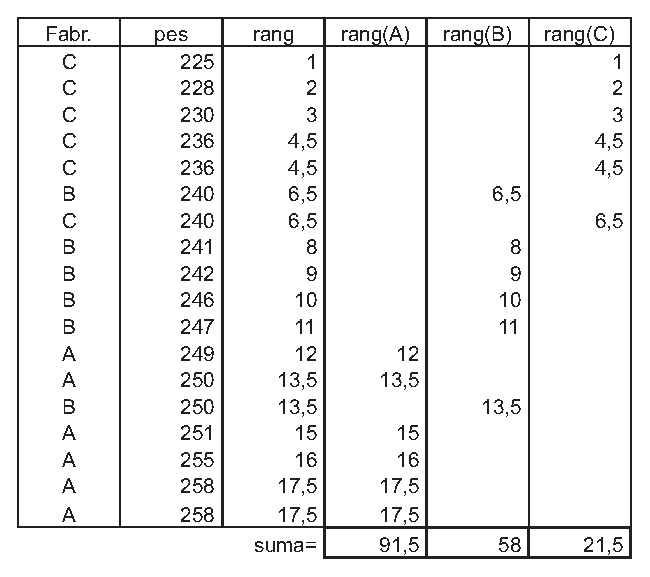
\includegraphics[width=7.2cm]{./imatges/tabla5.eps}
\end{center}
\caption{Taula per calcular $H$ amb les dades de l'exemple
\ref{example_nopara_10}}
\end{table}

L'estad�stic per al contrast �s
\[
H=\frac{12}{18\cdot
19}\left(\frac{91.5^2}{6}+\frac{58^2}{6}+\frac{21.5^2}{6}\right)-3\cdot
19=14.34
\]
El valor cr�tic per a un nivell de significaci� del 0.05 que
trobem a la taula de la khi-quadrat amb 2 graus de llibertat �s
5.99 i, com queda superat per l'estad�stic, rebutgem la igualtat
entre els fabricants. \par Encara que hi ha lligadures, en aquest
cas no cal calcular $H'>H$.

\section{Test de Friedman}

Aquest test est� pensat per comprovar si existeixen difer�ncies
significatives entre $k$ tractaments o condicions experimentals
aplicats a $n$ individus.
\begin{center}
\begin{tabular}{|c|cccccc|} \hline
 & \multicolumn{6}{c|}{Tractament}  \\ \hline
Individu & 1 & 2 & $\dots$ & $j$ & \dots & $k$  \\ \hline
 1   &  $x_{11}$ & $x_{12}$ & \dots & $x_{1j}$ & \dots & $x_{1k}$ \\
 2   &  $x_{21}$ & $x_{22}$ & \dots & $x_{2j}$ & \dots & $x_{2k}$ \\
 \vdots & \vdots & \vdots & & \vdots & & \vdots \\
 $n$ & $x_{n1}$ & $x_{n2}$ & \dots & $x_{nj}$ & \dots & $x_{nk}$ \\ \hline
\end{tabular}
\end{center}
Els individus s'han d'escollir a l'atzar i de forma independent,
de forma que les files s�n independents entre s�. Per�, com els
individus s�n els mateixos, les columnes s�n dependents.

El test de Friedman serveix per provar si hi ha difer�ncies entre
els $k$ tractaments (efecte columna), amb la pres�ncia dels
efectes individuals (efecte fila). �s una versi� no param�trica
del disseny de dos factors sense interacci�. �s clar que la
hip�tesi nu{\ll}a �s la igualtat de resposta o d'efecte dels
diferents tractaments, mentre que l'alternativa �s que hi ha, com
a m�nim, dos tractaments amb resposta diferent.

Per calcular l'estad�stic no param�tric, per cada fila per
separat, s'assignen els rangs que corresponen als valors
observats. Una vegada convertida la taula original en rangs, es
calculen les sumes de rangs $R_j$ per a cada columna o tractament
$j=1,\dots,k$. L'estad�stic �s
\[
S=\frac{12}{nk(k+1)}\sum_{j=1}^k R_j^2 -3n(k+1)
\]
La distribuci� aproximada de $S$ per a valors grans de $n$ �s una
khi-quadrat amb $k-1$ graus de llibertat. Per a valors molt petits
de $n$ ($n<10$) cal consultar unes taules especials. La regi�
cr�tica �s de la forma $\{S\ge c\}$.

Quan hi ha lligadures en una fila, s'han de promitjar els rangs
dels valors repetits i calcular l'estad�stic de Friedman modificat
per un factor de correcci�
\[
S'=\frac{12\sum_{j=1}^k R_j^2
-3n^2k(k+1)^2}{nk(k+1)-\frac{1}{k-1}\sum_{i=1}^n\left\{\sum_{j=1}^{g_i}
t_{ij}^3 -k\right\}}
\]
on $g_i$ �s el n�mero de grups d'observacions lligades en la fila
$i$ i $t_{ij}$ el n�mero d'observacions lligades en el grup $j$ de
la fila $i$. Quan no hi ha lligadures es considera per conveni que
$g_i=k$, $t_{ij}=1$, i llavors, el terme de correcci� pel individu
$i$ �s $\sum_{j=1}^{g_i} t_{ij}^3 -k=k-k=0$. Si aix� passa en
totes les files, llavors $S'=S$.

\begin{example}\label{example_nopara_14}
S'ha consultat a un grup de 12 persones per tal que opinin sobre
cinc marques de xamp�. En concret les seves classificacions es
troben a la seg�ent taula.
\begin{center}
\begin{tabular}{|c|ccccc|} \hline
 & \multicolumn{5}{c|}{Xamp�}  \\ \hline
Ind. & A & B & C & D & E \\ \hline
 1       & 5 & 3 & 2 & 4 & 1  \\
 2       & 4 & 3 & 5 & 2 & 1  \\
 3       & 3 & 5 & 4 & 2 & 1  \\
 4       & 4 & 5 & 1 & 2 & 3  \\
 5       & 3 & 4 & 5 & 1 & 2  \\
 6       & 5 & 3 & 4 & 2 & 1  \\
 7       & 2 & 5 & 4 & 3 & 1  \\
 8       & 3 & 5 & 4 & 1 & 2  \\
 9       & 3 & 4 & 5 & 2 & 1  \\
 10      & 4 & 5 & 3 & 1 & 2  \\
 11      & 5 & 3 & 2 & 4 & 1  \\
 12      & 5 & 4 & 3 & 2 & 1  \\ \hline
\end{tabular}
\end{center}
Esbrineu si hi ha difer�ncies significatives entre els xampus.
\end{example}

\textit{Soluci�:}

En aquest cas les dades de la taula coincideixen directament amb
els rangs i, a m�s, no hi ha lligadures. Les sumes dels rangs per
columnes s�n
\[
R_A=46 \quad R_B=49 \quad R_C=42 \quad R_D=26 \quad R_E= 17
\]
De forma que l'estad�stic �s
\[
S=\frac{12}{12\cdot 5\cdot 6}(46^2+49^2+42^2+26^2+17^2)-3\cdot
12\cdot 6=25.53
\]
Un valor clarament superior al de la taula de la khi-quadrat
$\chi^2_{4,0.05}=9.488$. Aix� hem de rebutjar la igualtat entre
els xampus.

\bigskip \textbf{Observacions}

\begin{itemize}
\item Es pot veure que
\[
S=\frac{12n}{k(k+1)}\sum_{j=1}^k (R_{\bullet
j}-R_{\bullet\bullet})^2
\]
on $R_{\bullet j}=R_j/n$ i $R_{\bullet\bullet}=(k+1)/2$. Aix�
posar de manifest la relaci� d'aquest test amb el test $F$ per
detectar l'efecte columna en el disseny de dos factors sense
interacci�.
\end{itemize}

\section{Test de ratxes}

En aquesta secci� ens plantegem si una mostra observada �s
realment una mostra aleat�ria simple, �s a dir, si les
observacions han estat plenament independents. Qualsevol condici�
de mostratge sense les degudes garanties d'aleatorietat pot
afectar a la independ�ncia. Per exemple, l'aprenentatge d'un
aparell de mesura pot modificar les observacions amb el temps.
Aquesta q�esti� �s molt important perqu� molts m�todes de contrast
que hem estudiat parteixen sempre de la consideraci� de mostres
aleat�ries simples.

Aix� doncs, la nostra intenci� �s contrastar les hip�tesis
\[
\begin{split}
H_0 &: \textrm{la mostra observada �s aleat�ria} \\
H_1 &: \textrm{la mostra observada no �s aleat�ria}
\end{split}
\]
Pensem en una variable aleat�ria que nom�s pren el valors $a$ i
$b$ i que observem les mostres
\[
aaaaaaaabbbbbb \qquad\textrm{�}\qquad ababababababab
\]
�s evident que presenten un aspecte poc aleatori. En canvi, la
sospita no apareix si, per exemple, les mostres observades s�n
\[
abbaaabbaabbba \qquad\textrm{�}\qquad baaabbabbbbaaa
\]
Una ratxa �s una s�rie de s�mbols id�ntics (o relacionats)
continguda entre dos s�mbols diferents o un de sol si estem al
principi o al final de la seq��ncia. Si, per exemple, separem les
ratxes amb una barra vertical tenim
\[
\begin{array}{ll}
aaaaaaaa|bbbbbb & \qquad a|b|a|b|a|b|a|b|a|b|a|b|a|b \\
a|bb|aaa|bb|aa|bbb|a & \qquad b|aaa|bb|a|bbbb|aaa
\end{array}
\]
En el primer cas hi ha dues ratxes, molt poques, i en el segon
masses, en realitat el n�mero m�xim. En canvi, els altres dos
casos s�n m�s naturals, m�s aleatoris. Sembla clar doncs que
existeix una relaci� entre el n�mero de ratxes i l'aleatorietat.
La seq��ncia es considera no aleat�ria quan hi ha masses o massa
poques ratxes.

Es pot estudiar la distribuci� en el mostratge del n�mero $R$ de
ratxes quan es formen totes les seq��ncies possibles amb $n_1$
s�mbols $a$ i $n_2$ s�mbols $b$. Es demostra que la mitjana i la
vari�ncia d'aquesta distribuci� s�n
\[
\mu_R=\frac{2n_1n_2}{n_1+n_2}+1 \qquad\qquad \sigma_R^2=
\frac{2n_1n_2(2n_1n_2-n_1-n_2)}{(n_1+n_2)^2(n_1+n_2-1)}
\]
Quan $n_1$ i $n_2$ s�n grans (superiors a 8) la distribuci�
asimpt�tica �s normal i per contrastar l'aleatorietat podem
utilitzar l'estad�stic
\[
z=\frac{R-\mu_R}{\sigma_R}
\]
amb una regi� cr�tica de dues cues.

\begin{example}\label{example_nopara_11}
Considerem els valors observats en la producci� d'una m�quina que
indiquem per $\,c$ quan la pe�a fabricada �s correcte i $\,d$ quan
�s defectuosa.
\[
\begin{array}{ccccccccccccccc}
c & c & c & c & d & d & c & c & c & c & c & c & c & c & c \\
c & d & d & d & c & c & c & c & c & c & c & c & c & c & c \\
c & c & d & c & c & c & c & c & c & d & d & c & c & c & c \\
c & c & d & c & c & c & d & d & c & c & c & c & c & c & c \\
c & c & c & c & c & c & c & c & c & c & d & d & d & c & c
\end{array}
\]
Apliqueu el test de les ratxes per comprovar l'aleatorietat
d'aquesta mostra.
\end{example}

\textit{Soluci�:}

El recompte de les ratxes per files ens diu que $R=15$ i $n_1=61,
n_2=14$. Aix� doncs, els par�metres de la distribuci� de $R$ s�n
\[
\begin{split}
\mu_R&=\frac{2\cdot 61\cdot 14}{61+14}+1=23.7733
 \\
\sigma_R^2&=\frac{2\cdot 61\cdot 14\cdot (2\cdot 61\cdot
14-61-14)}{(61+14)^2(61+14-1)} =6.7007
\end{split}
\]
i l'estad�stic $z=(15-\mu_R)/\sigma_R=-3.39$. Aquest valor cau a la
regi� cr�tica de dues cues de la distribuci� normal per al nivell
del 0.05, de manera que hem de posar en dubte l'aleatorietat de la
mostra. Les peces defectuoses apareixen de forma agrupada.

\subsection{Aleatorietat d'una mostra num�rica}

Per tal de determinar si una mostra de dades num�riques �s o no
aleat�ria, considerem la seq��ncia de dades tal com van ser
observades, �s a dir, en el mateix ordre. Calculem la mediana i
assignem el s�mbol $-$ o $+$ a cada observaci� en funci� que
aquest valor estigui per sota o per sobre de la mediana. Si un
valor coincideix amb la mediana el suprimirem, de forma que quasi
sempre resultar� $n_1=n_2=m$. L'aleatorietat de la mostra es
contrasta amb l'estad�stic $R$ amb par�metres
\[
\mu_R=m+1 \qquad\qquad \sigma_R^2= \frac{m(m-1)}{2m-1}
\]

\begin{example}\label{example_nopara_12}
Comproveu l'aleatorietat de les dades de l'exemple
\ref{example_nopara_1}.
\end{example}

\textit{Soluci�:}

La mediana de la mostra �s 70, de forma que s'obtenen els s�mbols
de la taula.
\[
\begin{array}{|cccccccccc|} \hline
  71 & 67 & 55 & 64 & 82 & 66 & 74 & 58 & 79 & 61 \\
  78 & 46 & 84 & 93 & 72 & 54 & 78 & 86 & 48 & 52 \\
  67 & 95 & 70 & 43 & 70 & 73 & 57 & 64 & 60 & 83 \\
  73 & 40 & 78 & 70 & 64 & 86 & 76 & 62 & 95 & 66 \\ \hline
  + & - & - & - & + & - & + & - & + & - \\
  + & - & + & + & + & - & + & + & - & - \\
  - & + &   & - &   & + & - & - & - & + \\
  + & - & + &   & - & + & + & - & + & - \\ \hline
\end{array}
\]
El recompte de les ratxes per files ens diu que $R=26$ i,
malauradament en aquest cas, els empats ens porten a $n_1=19\ne
n_2=18$. Aix� doncs, els par�metres de la distribuci� de $R$ s�n
\[
\begin{split}
\mu_R&=\frac{2\cdot 19\cdot 18}{19+18}+1=19.4865
 \\
\sigma_R^2&=\frac{2\cdot 19\cdot 18\cdot (2\cdot 19\cdot
18-19-18)}{(19+18)^2(19+18-1)} =8.9795
\end{split}
\]
i l'estad�stic $z=(26-\mu_R)/\sigma_R=2.17$. Aquest valor cau a la
regi� cr�tica de dues cues de la distribuci� normal per al nivell
del 0.05, de manera que hem de posar en dubte l'aleatorietat de la
mostra.

\bigskip
Una altra aplicaci� del test de ratxes consisteix en substituir
cada valor mostral, excepte el primer, per $-$ � $+$ segons que
aquest sigui inferior o superior a l'anterior. Aix� detectarem si
hi ha hagut per�odes d'observaci� amb tend�ncies de creixement o
decreixement, no atribu�bles a l'atzar.

\begin{example}\label{example_nopara_13}
Comproveu l'aleatorietat dels per�odes de creixement i
decreixement de les dades de l'exemple \ref{example_nopara_1}.
\end{example}

\textit{Soluci�:}

La seg�ent taula recull els s�mbols $-$ i $+$ que expressen si un
valor �s inferior o superior a l'anterior.
\[
\begin{array}{|cccccccccc|} \hline
  71 & 67 & 55 & 64 & 82 & 66 & 74 & 58 & 79 & 61 \\
  78 & 46 & 84 & 93 & 72 & 54 & 78 & 86 & 48 & 52 \\
  67 & 95 & 70 & 43 & 70 & 73 & 57 & 64 & 60 & 83 \\
  73 & 40 & 78 & 70 & 64 & 86 & 76 & 62 & 95 & 66 \\ \hline
    & - & - & + & + & - & + & - & + & - \\
  + & - & + & + & - & - & + & + & - & + \\
  + & + & - & - & + & + & - & + & - & + \\
  - & - & + & - & - & + & - & - & + & - \\ \hline
\end{array}
\]
El recompte de les ratxes per files ens proporciona $R=27$ per
$n_1=19$ i $n_2=20$. Tamb�, com en l'exemple anterior, �s evident
que el n�mero de ratxes �s excessiu.

\subsection{Comparaci� de dues mostres}

El test de les ratxes es pot aplicar tamb� a la comparaci� de dues
mostres independents, encara que proporciona un resultat m�s pobre
que el test $U$ de Mann-Whitney. La idea �s ordenar les dues
mostres de forma conjunta, assignar un s�mbol a la primera mostra
i un altre a la segona i, finalment, comptar les ratxes que en
resulten.

Si les dues mostres procedeixen de la mateixa distribuci�
poblacional, els seus valors haurien d'estar barrejats. En canvi,
si existeix una difer�ncia de posici� entre les distribucions
poblacionals, els signes estaran m�s agrupats i el n�mero de
ratxes ser� m�s redu�t. Aix� doncs, en aquest cas la regi� cr�tica
�s de la forma $\{R\le k\}$.

\subsection{Distribuci� exacta de $R$}

Suposem que a la mostra hi ha $n_1$ s�mbols $a$ i $n_2$ s�mbols
$b$. Llavors la distribuci� de $R$, tot suposant que la mostra �s
aleat�ria, es pot trobar expl�citament:
\[
\begin{split}
P(R=2r) &=
2\frac{\binom{n_1-1}{r-1}\binom{n_2-1}{r-1}}{\binom{n_1+n_2}{n_1}}
\\
P(R=2r+1)&=
\frac{\binom{n_1-1}{r-1}\binom{n_2-1}{r}+\binom{n_1-1}{r}\binom{n_2-1}{r-1}}%
{\binom{n_1+n_2}{n_1}}
\end{split}
\]
on $r\le\min\{n_1,n_2\}$.

En efecte, $n_1+n_2$ s�mbols es poden ordenar de $(n_1+n_2)!$
formes, igualment probables. Per formar seq��ncies amb $r$ ratxes
de $a$ i $r$ ratxes de $b$, les $a$ es poden ordenar de $n_1!$
formes, i dividir-se despr�s en $r$ grups, amb l'elecci� de $r-1$
dels $n_1-1$ forats existents entre ells. An�logament, les $b$
poden ser ordenades de $n_2!$ maneres i dividides en $r$ grups de
$\binom{n_2-1}{r-1}$ formes. Despr�s s'han d'intercalar els grups
formats, tot comen�ant amb el primer grup de $a$, o b� amb el
primer grup de $b$. En total, la probabilitat que hi hagi $r$
ratxes de cada tipus �s
\[
\frac{n_1!\binom{n_1-1}{r-1}n_2!\binom{n_2-1}{r-1}2}{(n_1+n_2)!}=
2\frac{\binom{n_1-1}{r-1}\binom{n_2-1}{r-1}}{\binom{n_1+n_2}{n_1}}
\]
De manera similar es calcula la probabilitat que hi hagi $r$
ratxes de $a$ i $r+1$ ratxes de $b$ i la probabilitat que hi hagi
$r+1$ ratxes de $a$ i $r$ ratxes de $b$. Aix� proporciona els dos
sumands de la segona expressi�. Naturalment, el n�mero de ratxes
d'un tipus i de l'altre es diferencien, com a molt, en 1.

\section{Coeficients de correlaci�}

En aquesta secci� proposem dos coeficients no param�trics que
permeten mesurar la depend�ncia estoc�stica de dues mostres
aparellades en poblacions cont�nues. Tamb� estem interessats en
els contrastos d'independ�ncia que es puguin formular amb aquests
coeficients.

\subsection{Coeficient $\tau$ de Kendall}

Considerem una mostra aleat�ria simple $(x_1,y_1),\dots,(x_n,y_n)$
d'una distribuci� bidimensional. Sabem que la freq��ncia relativa
de les parelles tals que $(x_i-x_j)(y_i-y_j)>0$ ser� un estimador
del par�metre
\[
\pi_{+}=P\{(X-X')(Y-Y')>0\}
\]
on $(X,Y)$ i $(X',Y')$ s�n independents i tenen la mateixa
distribuci� conjunta poblacional.

La continu�tat de les distribucions implica que
$P\{(X-X')(Y-Y')=0\}=0$, de manera que
\[
\pi_{-}=P\{(X-X')(Y-Y')<0\}=1-\pi_{+}
\]
Llavors,
\[
\tau=\pi_{+}-\pi_{-}=2\pi_{+}-1
\]
�s l'anomenat coeficient d'associaci� de Kendall i mesura, en
certa forma, la depend�ncia de les variables. De fet, si $X$ i $Y$
s�n independents,
\[
\begin{split}
\pi_{+}&=P(X<X')P(Y<Y')+P(X>X')P(Y>Y') \\
&= P(X>X')P(Y<Y')+P(X<X')P(Y>Y')=\pi_{-}
\end{split}
\]
de forma que $\tau=0$. El rec�proc no �s cert, pot ser $\tau=0$
sense que necess�riament les dues variables $X$ i $Y$ siguin
independents.

Si $P$ i $N$ representen el n�mero de parelles tals que
$(x_i-x_j)(y_i-y_j)>0$ i $(x_i-x_j)(y_i-y_j)<0$ respectivament,
entre les $\binom{n}{2}$ possibles, l'estimador natural de $\tau$
�s
\[
T=\frac{P}{\binom{n}{2}}-\frac{N}{\binom{n}{2}}=\frac{2}{n(n-1)}(P-N)
\]
Per� a m�s, sabem que $P+N=\binom{n}{2}$ i llavors
\[
T=\frac{4P}{n(n-1)} -1
\]
Per a una mostra concreta, $P$ es calcula f�cilment amb la mostra
ordenada per la primera component: �s el n�mero de parelles amb
$i<j$ per a les que $y_i<y_j$.

L'estad�stic $T$ pren valors entre $-1$ i $1$ i un valor lluny�
del zero ens indica que $\tau\ne 0$ i, per tant, que les variables
$X$ i $Y$ no s�n independents.

La distribuci� exacta de $T$ es pot calcular per a valors moderats
de $n$. Per a $n\le 10$ hi ha una taula de valors cr�tics tals que
$P(|T|>k_{\alpha})\le\alpha$. Per a $n>10$ pot considerar-se la
distribuci� aproximada
\[
T\sim N\left(0,\sqrt{\frac{2(2n+5)}{9n(n-1)}}\right)
\]

\begin{example}\label{example_nopara_15}
La longitud i l'amplada d'una mostra de 11 fulles d'una certa
planta �s
\begin{footnotesize}
\begin{center}
\begin{tabular}{lrrrrrrrrrrrr}
  \hline
  % after \\: \hline or \cline{col1-col2} \cline{col3-col4} ...
Fulla & 1 & 2 & 3 & 4 & 5 & 6 & 7 & 8 & 9 & 10 & 11 \\
  \hline
Long. & 6.60 & 7.11 & 9.80 & 6.62 & 7.10 & 6.83 & 6.54 & 7.14 & 7.13 & 12.52 & 10.41 \\
Ampl. & 4.24 & 5.41 & 5.26 & 5.53 & 3.25 & 4.22 & 3.98 & 3.29 & 3.43 &  5.57 &  6.01 \\
  \hline
\end{tabular}
\end{center}
\end{footnotesize}
Trobeu el coeficient de correlaci� de Kendall i estudieu si �s
significatiu.
\end{example}

\textit{Soluci�:}

Si ordenem les parelles per la primera component, l'ordenaci� de
les $y_i$ �s
\begin{center}
3.98\ 4.24\ 5.53\ 4.22\ 3.25\ 5.41\ 3.43\ 3.29\ 5.26\ 6.01\ 5.57
\end{center}
D'aquesta forma el recompte de les parelles tals que
$(x_i-x_j)(y_i-y_j)>0$ �s
\[
P=7+5+2+4+6+2+3+3+2+0=34
\]
Aix� tenim
\[
T=\frac{4\cdot 34}{11\cdot 10} -1=0.2364
\]
Es pot comprovar que aquest valor no �s suficient per rebutjar la
hip�tesi d'independ�ncia.


\subsection{Coeficient de correlaci� per rangs de Spearman}

El coeficient de correlaci� de Spearman �s el coeficient de
correlaci� ordinari, anomenat correlaci� de Pearson, si substitu�m
les parelles de valors $(x_1,y_1),\dots,(x_n,y_n)$ pels seus
rangs. El resultat �s
\[
r_S=1-\frac{6\sum_{i=1}^n d_i^2}{n(n^2-1)}
\]
on $d_i=r(x_i)-r(y_i)$, $i=1,\dots,n$ s�n les difer�ncies dels
rangs dels valors en les seves respectives mostres.

Aquest coeficient s'utilitza quan les variables s�n mesurades en
una escala ordinal i l'ordre en la mostra �s la informaci� m�s
rellevant.

\subsubsection{C�lcul del coeficient}

Com hem dit, el coeficient de correlaci� $r_S$ de Spearman �s el
coeficient de correlaci� ordinari en substituir els valors
mostrals $(x_1,y_1),\dots,$ $(x_n,y_n)$ per
$(a_1,b_1),\dots,(a_n,b_n)$, on $a_i=r(x_i)$ �s el rang de la dada
$x_i$ quan hem ordenat les $x$ i $b_i=r(y_i)$ el rang que ocupa
$y_i$ en l'ordenaci� creixent de les $y$.

Efectivament,
\[
r_S=\frac{\sum_{i=1}^n(a_i-\bar{a})(b_i-\bar{b})}%
{\sqrt{\sum_{i=1}^n(a_i-\bar{a})^2\sum_{i=1}^n(b_i-\bar{b})^2}}
\]
on $\bar{a}=\bar{b}=(1/n)\sum_{i=1}^n i=(n+1)/2$\quad i
\[
\sum_{i=1}^n(a_i-\bar{a})^2=\sum_{i=1}^n(b_i-\bar{b})^2=
\sum_{i=1}^n i^2 -n\frac{(n+1)^2}{4}=\frac{n(n^2-1)}{12}
\]
de manera que
\[
r_S=\frac{n(n^2-1)}{12}\sum_{i=1}^n(a_i-\bar{a})(b_i-\bar{b})
\]
D'altra banda
\[
\begin{split}
\sum_{i=1}^n d_i^2 &= \sum_{i=1}^n (a_i-b_i)^2 =\sum_{i=1}^n
(a_i-\bar{a}+\bar{b}-b_i)^2 \\
&=\frac{n(n^2-1)}{6}-2\sum_{i=1}^n(a_i-\bar{a})(b_i-\bar{b}) \\
&=\frac{n(n^2-1)}{6}-2\frac{n(n^2-1)}{12}r_S=\frac{n(n^2-1)}{6}(1-r_S)
\end{split}
\]
d'on resulta l'expressi� amb la que hem definit el coeficient
$r_S$.

Sota la hip�tesi d'independ�ncia es pot calcular la distribuci� en
el mostratge de $r_S$ i, per tant, es pot determinar els punts
cr�tics del contrast per a diferents nivells de significaci� i
$n\le 10$. Per a $n>10$, pot provar-se que $r_S$ es aproximadament
$N(0,1/\sqrt{n-1})$.

\begin{example}\label{example_nopara_16}
Calculeu el coeficient de correlaci� per rangs de Spearman per a
les dades de l'exemple \ref{example_nopara_15} i estudieu si �s
significatiu.
\end{example}

\textit{Soluci�:}

Si juguem amb l'ordenaci� dels valors i els seus rangs tenim
\begin{table}[h]\label{taula_excel6}
\begin{center}
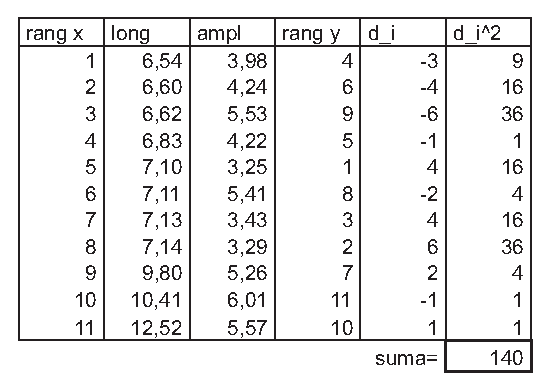
\includegraphics[width=7.2cm]{./imatges/tabla6.eps}
\end{center}
\caption{Taula per a la suma de les difer�ncies al quadrat dels
rangs de l'exemple \ref{example_nopara_16}}
\end{table}

El resultat �s $\sum_{i=1}^n d_i^2=140$ i per tant
\[
r_S=1-\frac{6\cdot 140}{11(11^2-1)}=0.3636
\]
Aquest valor no �s suficient per rebutjar la independ�ncia entre
les variables.

\subsubsection{El par�metre poblacional}
Si la distribuci� conjunta de $(X,Y)$ �s $F(x,y)$ i les
distribucions marginals s�n $F_X(x)$ i $F_Y(y)$, llavors $\rho_S$
�s el coeficient de correlaci� ordinari entre les variables
$V_1=F_X(X)$ i $V_2=F_Y(Y)$ amb distribuci� uniforme totes dues.
Amb conseq��ncia es pot provar que
\[
\begin{split}
\rho_S &= 12 \iint_{\mathbb{R}^2}
(F(x,y)-F_X(x)F_Y(y))\,dF_X(x)dF_Y(y) \\
&=12 \iint_{\mathbb{R}^2} F(x,y)\,dF_X(x)dF_Y(y)-3
\end{split}
\]

La versi� probabil�stica de la correlaci� $\tau$ de Kendall �s
\[
\tau=4 \int_{\mathbb{R}^2}(F(x,y)-F_X(x)F_Y(y))\,dF(x,y)
\]
i es verifica la relaci�
\[
-1\le 3\tau-2\rho_S\le 1
\]
Observem que $\rho_S=\tau=0$ si $F(x,y)=F_X(x)F_Y(y)$, �s a dir,
si $X,Y$ s�n estoc�sticament independents.

Per contrastar la hip�tesi nu{\ll}a $H_0:\rho_S=0$, on $\rho_S$ �s
la correlaci� poblacional, podem calcular l'estad�stic
\[
t=\sqrt{n-2} \frac{r_S}{\sqrt{1-r_S^2}}
\]
que t� una distribuci� aproximada (si $n\ge 10$) $t$ de Student
amb $n-2$ graus de llibertat.

\section{Soluci� de problemes amb R o S-PLUS}

\subsubsection{Exemple \ref{example_nopara_1}}

Primer introdu�m les notes i calculem quants valors s�n superiors
a 66, �s a dir, el n�mero de signes positius.
\begin{footnotesize}
\begin{verbatim}
> notes<-c(71,67,55,64,82,66,74,58,79,61,78,46,84,93,72,54,78,86,48,52,67,
  95,70,43,70,73,57,64,60,83,73,40,78,70,64,86,76,62,95,66)
> notes[notes>66]
 [1] 71 67 82 74 79 78 84 93 72 78 86 67 95 70 70 73 83 73 78 70 86 76 95
> B<-length(notes[notes>66])
> B
[1] 23
\end{verbatim}
\end{footnotesize}
I finalment, calculem l'aproximaci� normal de l'estad�stic i el
seu p-valor.
\begin{footnotesize}
\begin{verbatim}
> n<-length(notes)-length(notes[notes==66])
> n
[1] 38
> z<-(B-0.5-n*0.5)/sqrt(n*0.5*0.5)
> round(z,2)
[1] 1.14
> 2*(1-pnorm(z))
[1] 0.2561450
> 2*(1-pnorm(B-0.5,mean=n*0.5,sd=sqrt(n*0.5*0.5)))
[1] 0.2561450
\end{verbatim}
\end{footnotesize}
El p-valor superior al nivell de significaci� fa que acceptem la
hip�tesi nu{\ll}a $H_0:M=66$.

\subsubsection{Exemple \ref{example_nopara_2}}

Introdu�m les dades en dos vectors de la mateixa longitud.
Calculem la difer�ncia i el n�mero de valors positius. A partir
d'aquest n�mero, calculem la probabilitat de la cua dreta d'una
binomial, ja que la hip�tesi alternativa aix� ho demana.
\begin{footnotesize}
\begin{verbatim}
> maq1<-c(46,110,70,54,60,120,82,76,37,28)
> maq2<-c(42,87,75,50,48,108,80,67,40,25)
> dif<-maq1-maq2
> dif
 [1]  4 23 -5  4 12 12  2  9 -3  3
> B<-length(dif[dif>0]);B
[1] 8
> dbinom(8,10,0.5)+dbinom(9,10,0.5)+dbinom(10,10,0.5)
[1] 0.0546875
> 1-pbinom(B-1,10,0.5)
[1] 0.0546875
\end{verbatim}
\end{footnotesize}
El p-valor �s inferior al nivell de significaci� 0.06 i, per tant,
rebutgem la hip�tesi nu{\ll}a i acceptem que la m�quina 1 produeix
m�s peces defectuoses.

\subsubsection{Exemple \ref{example_nopara_3}}

En aquest cas els c�lculs s�n molt senzills.
\begin{footnotesize}
\begin{verbatim}
> z<-(197-0.5-300*0.5)/sqrt(300*0.5*0.5);z
[1] 5.369358
> 1-pnorm(z)
[1] 3.950882e-08
\end{verbatim}
\end{footnotesize}
I el p-valor �s clarament inferior a 0.01, de manera que acceptem
l'alternativa.

\subsubsection{Exemple \ref{example_nopara_4}}

En aquest exemple farem servir la funci� \texttt{wilcox.test} amb
el vector \texttt{notes} de l'exemple \ref{example_nopara_1}.
\begin{footnotesize}
\begin{verbatim}
> wilcox.test(notes,mu=66,alternative="two.sided",exact=F)

        Wilcoxon signed rank test with continuity correction

data:  notes
V = 465, p-value = 0.1726
alternative hypothesis: true mu is not equal to 66
> z<-(465-0.5-38*39/4)/sqrt(38*39*77/24);z
[1] 1.363214
> round(2*(1-pnorm(z)),2)
[1] 0.17
\end{verbatim}
\end{footnotesize}

Aquesta funci� calcula l'estad�stic $T^{+}=465$ i el seu p-valor
amb correcci� per continu�tat. En aquest problema hi ha, a m�s de
dos zeros, un grapat d'empats o lligadures, de manera que la
funci� \texttt{wilcox.test} no pot calcular el p-valor exacte i
per aix� li hem indicat amb \texttt{exact=F}. L'estad�stic $z$ que
hem calculat de forma directa i el seu p-valor, sense tenir en
compte les lligadures, s�n for�a semblants als que l'algorisme
calcula. Si no indiquem res sobre aquest par�metre, sortiran dos
missatges d'advert�ncia sobre aquest fet.
\begin{footnotesize}
\begin{verbatim}
> wilcox.test(notes,mu=66,alternative="two.sided")

        Wilcoxon signed rank test with continuity correction

data:  notes
V = 465, p-value = 0.1726
alternative hypothesis: true mu is not equal to 66

Warning messages:
1: Cannot compute exact p-value with ties in:
   wilcox.test.default(x, mu = 66, alternative = "two.sided")
2: Cannot compute exact p-value with zeroes in:
   wilcox.test.default(x, mu = 66, alternative = "two.sided")
\end{verbatim}
\end{footnotesize}
M�s informaci� sobre la funci� amb
\begin{footnotesize}
\begin{verbatim}
> help(wilcox.test)
\end{verbatim}
\end{footnotesize}

\subsubsection{Exemple \ref{example_nopara_5}}

En aquest exemple tamb� s'utilitza la funci� \texttt{wilcox.test}
amb els dos vectors de dades de l'exemple \ref{example_nopara_2}.
\begin{footnotesize}
\begin{verbatim}
> wilcox.test(maq1,maq2,mu=0,paired=T,alternative="greater",exact=F)

        Wilcoxon signed rank test with continuity correction

data:  maq1 and maq2
V = 46.5, p-value = 0.02942
alternative hypothesis: true mu is greater than 0
\end{verbatim}
\end{footnotesize}
Observem que en aquest cas hem fet servir l'opci�
\texttt{paired=T} per indicar que les dades s�n aparellades. Tamb�
hem identificat l'alternativa correcte amb
\texttt{alternative="greater"}. A m�s, com en l'exemple anterior,
les lligadures no permeten calcular el p-valor exacte. El p-valor
aproximat 0.029 ens indica el rebuig de la hip�tesi nu{\ll}a.

\subsubsection{Exemple \ref{example_nopara_6}}

Ara farem servir la funci� \texttt{wilcox.test} amb els dos
vectors de dades per� tindrem en compte que s�n independents, que
�s l'opci� per defecte.
\begin{footnotesize}
\begin{verbatim}
> pro.A<-c(202,229,215,220,223,233,208,228,209)
> pro.B<-c(221,207,185,203,187,190,195,204,212)
> wilcox.test(pro.A,pro.B,alternative="two.sided")

        Wilcoxon rank sum test

data:  pro.A and pro.B
W = 70, p-value = 0.007775
alternative hypothesis: true mu is not equal to 0
\end{verbatim}
\end{footnotesize}
No ens hem de deixar confondre per la notaci�, l'estad�stic
calculat �s el que nosaltres hem anomenat $U'=70>n_1n_2/2=40.5$.
En tot cas, el p-valor �s molt expl�cit i implica el rebuig de la
hip�tesi nu{\ll}a d'equival�ncia.

\subsubsection{Exemple \ref{example_nopara_7}}

Observem el c�lcul de la mediana conjunta amb
\texttt{median(c(pro.A,pro.B))}.
\begin{footnotesize}
\begin{verbatim}
> T<-length(pro.A[pro.A<median(c(pro.A,pro.B))])
> T
[1] 2
> phyper(T,9,9,9)
[1] 0.02834225
> 1-phyper(6,9,9,9)
[1] 0.02834225
\end{verbatim}
\end{footnotesize}
La distribuci� hipergeom�trica ens permet trobar els l�mits de la
regi� cr�tica.

\subsubsection{Exemple \ref{example_nopara_8}}

En primer lloc hem d'introduir les freq��ncies de la taula.
\begin{footnotesize}
\begin{verbatim}
> numero<-cbind(expand.grid(M=c("inferior a M","superior a M"),
  grup=c("A","B")))
> fr<-c(2,7,7,2)
> attach(numero)
> taula<-table(M,grup)*fr
> taula
              grup
M              A B
  inferior a M 2 7
  superior a M 7 2
\end{verbatim}
\end{footnotesize}
I amb aquesta taula calculem el test d'homogene�tat.
\begin{footnotesize}
\begin{verbatim}
> chisq.test(taula)

        Pearson's Chi-squared test with Yates' continuity correction

data:  taula
X-squared = 3.5556, df = 1, p-value = 0.05935

Warning message:
Chi-squared approximation may be incorrect in: chisq.test(taula)
\end{verbatim}
\end{footnotesize}
El resultat �s l'acceptaci� de la igualtat de medianes. La
discrep�ncia amb l'exemple anterior �s possible per la manca
d'observacions.

\subsubsection{Exemple \ref{example_nopara_9}}

Les dades han estat introdu�des en els vectors \texttt{pro.A} i
\texttt{pro.B} i el test es calcula amb la funci�
\texttt{ks.test}.

\begin{footnotesize}
\begin{verbatim}
> ks.test(pro.A,pro.B,alternative="two.sided")

        Two-sample Kolmogorov-Smirnov test

data:  pro.A and pro.B
D = 0.6667, p-value = 0.03357
alternative hypothesis: two.sided
\end{verbatim}
\end{footnotesize}
En aquest cas, el p-valor ens indica el rebuig de la hip�tesi nu{\ll}a.

\subsubsection{Exemple \ref{example_nopara_10}}

Per fer el test de Kruskal-Wallis fem servir la funci�
\texttt{kruskal.test} que ens proporciona l'estad�stic $H$ o si
cal, com en aquest cas, l'estad�stic $H'$.
\begin{footnotesize}
\begin{verbatim}
> pes<-c(251,250,249,255,258,258,247,246,250,241,240,242,
  228,236,240,225,236,230)
> fabr<-c(rep(1,6),rep(2,6),rep(3,6))
> kruskal.test(pes,fabr)

        Kruskal-Wallis rank sum test

data:  pes and fabr
Kruskal-Wallis chi-squared = 14.3957, df = 2, p-value = 0.0007482
\end{verbatim}
\end{footnotesize}
El p-valor es prou significatiu del rebuig de la hip�tesi
nu{\ll}a.

\subsubsection{Exemple \ref{example_nopara_14}}

El test de Friedman s'aplica amb la funci� \texttt{friedman.test}.

\begin{footnotesize}
\begin{verbatim}
> nota<-c(5,3,2,4,1,4,3,5,2,1,3,5,4,2,1,
          4,5,1,2,3,3,4,5,1,2,5,3,4,2,1,
          2,5,4,3,1,3,5,4,1,2,3,4,5,2,1,
          4,5,3,1,2,5,3,2,4,1,5,4,3,2,1)
> individu<-c(rep(1,5),rep(2,5),rep(3,5),
              rep(4,5),rep(5,5),rep(6,5),
              rep(7,5),rep(8,5),rep(9,5),
              rep(10,5),rep(11,5),rep(12,5))
> xampu<-c(rep(seq(1,5,1),12))
> friedman.test(nota,xampu,individu)

        Friedman rank sum test

data:  nota, xampu and individu Friedman chi-squared = 25.5333, df
= 4, p-value = 3.929e-05
\end{verbatim}
\end{footnotesize}
El p-valor ens indica clarament la significaci� de les
difer�ncies.

\subsubsection{Exemple \ref{example_nopara_11}}

\begin{footnotesize}
\begin{verbatim}
> peces<-c(0,0,0,0,1,1,0,0,0,0,0,0,0,0,0,
           0,1,1,1,0,0,0,0,0,0,0,0,0,0,0,
           0,0,1,0,0,0,0,0,0,1,1,0,0,0,0,
           0,0,1,0,0,0,1,1,0,0,0,0,0,0,0,
           0,0,0,0,0,0,0,0,0,0,1,1,1,0,0)
> c<-1
> for (i in 1:(length(peces)-1)) if (peces[i]!=peces[i+1]) c<-c+1
> c
[1] 15
> n2<-sum(peces);n2
[1] 14
> n1<-length(peces)-n2;n1
[1] 61
> mu<-(2*n1*n2)/(n1+n2)+1;mu
[1] 23.77333
> sigma2<-(2*n1*n2*(2*n1*n2-n1-n2))/((n1+n2)^2*(n1+n2-1));sigma2
[1] 6.700694
> z<-(c-mu)/sqrt(sigma2);z
[1] -3.389259
> 2*pnorm(z)
[1] 0.0007008184
\end{verbatim}
\end{footnotesize}

Tamb� podem construir un test.
\begin{footnotesize}
\begin{verbatim}
> ratxes.test<-function(s){
+ c<-1
+ for (i in 1:(length(s)-1)) if (s[i]!=s[i+1]) c<-c+1
+ n2<-sum(s)
+ n1<-length(s)-n2
+ mu<-(2*n1*n2)/(n1+n2)+1
+ sigma2<-(2*n1*n2*(2*n1*n2-n1-n2))/((n1+n2)^2*(n1+n2-1))
+ z<-(c-mu)/sqrt(sigma2);z
+ }
> ratxes.test(peces)
[1] -3.389259
\end{verbatim}
\end{footnotesize}

\subsubsection{Exemple \ref{example_nopara_12}}

Calculem la mediana del vector \texttt{notes} i, per estalviar-nos
dificultats, eliminem del vector de dades els valors que
coincideixen amb la mediana.
\begin{footnotesize}
\begin{verbatim}
> median(notes)
[1] 70
> notes2<-c(71,67,55,64,82,66,74,58,79,61,78,46,84,93,72,54,78,86,48,52,67,
  95,43,73,57,64,60,83,73,40,78,64,86,76,62,95,66)
> signes<-ifelse(notes2<median(notes),0,1);signes
 [1] 1 0 0 0 1 0 1 0 1 0 1 0 1 1 1 0 1 1 0 0 0 1 0 1 0 0 0 1 1 0 1 0 1 1 0 1 0
> z<-ratxes.test(signes);z
[1] 2.173642
> 2*(1-pnorm(z))
[1] 0.029732
\end{verbatim}
\end{footnotesize}


\subsubsection{Exemple \ref{example_nopara_13}}

Tenim les dades en el vector \texttt{notes}
\begin{footnotesize}
\begin{verbatim}
> notes
 [1] 71 67 55 64 82 66 74 58 79 61 78 46 84 93 72 54 78 86 48 52 67 95 70 43 70
[26] 73 57 64 60 83 73 40 78 70 64 86 76 62 95 66
> notes2<-notes[2:length(notes)]
> cre<-ifelse(notes[1:(length(notes)-1)]<=notes2,1,0);cre
 [1] 0 0 1 1 0 1 0 1 0 1 0 1 1 0 0 1 1 0 1 1 1 0 0 1 1 0 1 0 1 0 0 1 0 0 1 0 0 1
[39] 0
> z<-ratxes.test(cre);z
[1] 2.115198
> 2*(1-pnorm(z))
[1] 0.03441305
\end{verbatim}
\end{footnotesize}

\subsubsection{Exemple \ref{example_nopara_15}}

Pel c�lcul dels coeficients de correlaci� s'utilitza la funci�
\texttt{cor.test} amb el par�metre
\begin{footnotesize}
\begin{center}
\texttt{method = c("pearson", "kendall", "spearman")"}
\end{center}
\end{footnotesize}
segons si volem el coeficient cl�ssic de Pearson, la $\tau$ de
Kendall o el coeficient per rangs de Spearman.
\begin{footnotesize}
\begin{verbatim}
> long<-c(6.60,7.11,9.80,6.62,7.10,6.83,6.54,7.14,7.13,12.52,10.41)
> ampl<-c(4.24,5.41,5.26,5.53,3.25,4.22,3.98,3.29,3.43,5.57,6.01)
> cor.test(long,ampl,method="kendall")

        Kendall's rank correlation tau

data:  long and ampl
T = 34, p-value = 0.3587
alternative hypothesis: true tau is not equal to 0
sample estimates:
      tau
0.2363636
\end{verbatim}
\end{footnotesize}
Observem que el n�mero de parelles {\em positives} �s 34,
estad�stic que nosaltres hem anomenat $P$.

El procediment calcula el p-valor exacte per a $n<50$. En aquest
cas el p-valor ens mostra que l'estad�stic no �s significatiu.

\subsubsection{Exemple \ref{example_nopara_16}}

Amb les dades de l'exemple \ref{example_nopara_15} tenim:
\begin{footnotesize}
\begin{verbatim}
> cor.test(long,ampl,method="spearman")

        Spearman's rank correlation rho

data:  long and ampl
S = 140, p-value = 0.2732
alternative hypothesis: true rho is not equal to 0
sample estimates:
      rho
0.3636364
\end{verbatim}
\end{footnotesize}

\section{Taules}

\begin{itemize}
\item  \textbf{Taula de probabilitats binomials:} D. Pe�a.
Estad�stica. Modelos y m�todos. Vol. I. Alianza Universidad. Tabla
2. p�g. 333

\item  \textbf{Taula de Wilcoxon:} C.M. Cuadras. Problemas de
probabilidades y Estad�stica Vol II. Tablas Estad�sticas. Tabla
XIV.

\item  \textbf{Taula de l'estad�stic $U$ de Mann-Whitney:} C.M.
Cuadras. Problemas de probabilidades y Estad�stica Vol II. Tablas
Estad�sticas. Tabla XII.

\item \textbf{Taula de Massey per al test d'homogene�tat de
Kolmogorov-Smirnov:} R. V�lez Ibarrola y A. Garc�a P�rez. C�lculo
de Probabilidades y Estad�stica Matem�tica. Principios de
Inferencia Estad�stica. UNED. Tablas 9 y 10.

\item \textbf{Taula de l'estadistic $\tau$ de Kendall:} R. V�lez
Ibarrola y A. Garc�a P�rez. C�lculo de Probabilidades y
Estad�stica Matem�tica. Principios de Inferencia Estad�stica.
UNED. Tabla 13.

\item \textbf{Taula de l'estadistic $r_S$ de Spearman:} R. V�lez
Ibarrola y A. Garc�a P�rez. C�lculo de Probabilidades y
Estad�stica Matem�tica. Principios de Inferencia Estad�stica.
UNED. Tabla 14.
\end{itemize}


\begin{thebibliography}{99}

%\newcommand{\citalib}[6]{\bibitem{#1} #2\ (#3).\ {\em{ #4}}.\  #5. \ #6.}
%\citalib{Alcaide-92}     %paraula clau per a la cita
%{Alcaide, J.}            %autors
%{1996}                   %any
%{Metodolog!`a de la prog} %Titol
%{Mc Graw-Hill}           %Editorial
%{Madrid}                 %Lloc

\citalib{Canavos-88} %Nom Clau
{Canavos, George C.} %Autors
{1988} % Any
{Probabilidad y Estadistica. Aplicaciones y Metodos}
{McGraw-Hill/Interamericana}
{Mexico}

\citalib{Cuadras-00} %Nom Clau
{Cuadras, C.M.} %Autors
{2000} % Any
{Problemas de probabilidades y estad\'{\i}stica. Vol. 2: Inferencia
estad\'{\i}stica} {EUB. Econom\'{\i}a y Empresa}{Barcelona}

\citalib{DeGroot-88} %Nom Clau
{De Groot, M.} %Autors
{1988} % Any
{Probabilidad y Estad\'{\i}stica}{Addison-Wesley}{}

\citalib{Casella-90} %Nom Clau
{Casella, G. Berger, M} %Autors
{1990} % Any
{Statistical inference}{Duxbury Press}{}

\citalib{Dudewicz-89} %Nom Clau
{Dudewicz, Edward J., Mishra, S.} %Autors
{1989} % Any
{Modern mathematical statistics} {John Wiley \& Sons, Wiley
series in probability and statistics} {New York}

\citalib{Fortiana-99} %Nom Clau
{Fortiana, J., Nualart, D.}%Autors
{1999} % Any
{Estad\'{\i}stica}
{Publicacions de la Universitat de
Barcelona}{Barcelona}

\citalib{Lehman-86} %Nom Clau
{Lehman, E.} %Autors
{1986} % Any
{Testing Statistical Hypothesis}
{John Wiley \& Sons, Wiley series in probability and statistics}
{New York}

\citalib{Martinez-93} %Nom Clau
{Mart\'{\i}nez A., Rodriguez, C., Guti\'{e}rrez, R} %Autors
{1993} % Any
{Inferencia Estadistica, un Enfoque Clasico} {Ediciones Pir\'{a}mide,
Economia y Administraci\'{o}n de Empresas}{Madrid}

\citalib{Penya-87a} %Nom Clau
{Pe\~{n}a, Daniel} %Autors
{1987} % Any
{Estad\'{\i}stica modelos y metodos 1. Fundamentos} {Alianza
editorial}
{Madrid}

\citalib{Rohatgi-75} %Nom Clau
{Rohatgi, V. K.} %Autors
{1976} % Any
{An Introduction to Probability Theory and Mathematical
Statistics}{John Wiley \& Sons, Wiley Series in Probability}{New
York}

\citalib{Ruiz-Maya-95} %Nom Clau
{Ruiz-Maya, L., Mart\'{\i}n Pliego, J.} %Autors
{1995} % Any
{Estad\'{\i}stica II: Inferencia}{Editorial AC. Colecci\'{o}n Plan
Nuevo}{Madrid}

\citalib{Sanz-99} %Nom Clau
{Sanz, Marta} %Autors
{1999} % Any
{Probabilitats}{Edicions de la UNiversitat de Barcelona}{Barcelona}

\citalib{Velez-93} %Nom Clau
{V�lez Ibarrola, Ricardo, Garcia Perez, Alfonso} %Autors
{1993} % Any
{Principios de Inferencia estad\'{\i}stica}{Editorial
UNED}{Madrid}

\end{thebibliography}

\end{document}
